%# -*- coding: utf-8-unix -*-
%======================================================================
% qbook.tex for Qbook Template
%======================================================================
% 双面打印
\documentclass{qbook}
\usepackage{ctex}
\usepackage{amsmath}
\usepackage{amssymb}

\addbibresource{bib/qbook.bib}  % 导入参考文献数据库

\begin{document}
\pagestyle{empty}
%# -*- coding: utf-8-unix -*-
\thispagestyle{empty}
\begin{tikzpicture}[overlay,remember picture,font=\sffamily\bfseries]
\draw[ultra thick,c4,name path=big arc] ([xshift=-2mm]current page.north) arc(150:285:11)
coordinate[pos=0.225] (x0);
\begin{scope}
\clip ([xshift=-2mm]current page.north) arc(150:285:11) --(current page.north
east);
\fill[c4!50,opacity=0.25] ([xshift=4.55cm]x0) circle (4.55);
\fill[c4!50,opacity=0.25] ([xshift=3.4cm]x0) circle (3.4);
\fill[c4!50,opacity=0.25] ([xshift=2.25cm]x0) circle (2.25);
\draw[ultra thick,c4!50] (x0) arc(-90:30:6.5);
\draw[ultra thick,c4] (x0) arc(90:-30:8.75);
\draw[ultra thick,c4!50,name path=arc1] (x0) arc(90:-90:4.675);
\draw[ultra thick,c4!50] (x0) arc(90:-90:2.875);
\path[name intersections={of=big arc and arc1,by=x1}];
\draw[ultra thick,c4,name path=arc2] (x1) arc(135:-20:4.75);
\draw[ultra thick,c4!50] (x1) arc(135:-20:8.75);
\path[name intersections={of=big arc and arc2,by={aux,x2}}];
\draw[ultra thick,c4!50] (x2) arc(180:50:2.25);
\end{scope} 
\path[decoration={text along path,text color=c4,
	raise = -2.8ex,
	text  along path,
	text = {|\sffamily\bfseries|\today},
	text align = center,
},
decorate
] ([xshift=-2mm]current page.north) arc(150:245:11);
%
\begin{scope}
\path[clip,postaction={fill=c3}]
([xshift=2cm,yshift=-8cm]current page.center) rectangle ++ (4.2,7.7);
\fill[c2] ([xshift=0.5cm,yshift=-8cm]current page.center)
([xshift=0.5cm,yshift=-8cm]current page.center)  arc(180:60:2)
|- ++ (-3,6) --cycle;
\draw[ultra thick,c4] ([xshift=-1.5cm,yshift=-8cm]current page.center) 
arc(180:0:2);
\draw[ultra thick,c4] ([xshift=0.5cm,yshift=-8cm]current page.center) 
arc(180:0:2);
\draw[ultra thick,c4] ([xshift=2.5cm,yshift=-8cm]current page.center) 
arc(180:0:2);
\draw[ultra thick,c4] ([xshift=4.5cm,yshift=-8cm]current page.center) 
arc(180:0:2);
\fill[red] ([xshift=2.5cm,yshift=-8cm]current page.center) +(60:2) circle(1.5mm);
\node[text=c5!80!black] at ([xshift=4.7cm,yshift=-5.2cm]current page.center) {$\rho:=\dfrac{1+\sqrt{-3}}{2}$};
\end{scope}
%
\fill[c1] ([xshift=2cm,yshift=-8cm]current page.center) rectangle ++ (-13.7,7.7);
\node[text=white,anchor=west,scale=4,inner sep=0pt] at
([xshift=-10.55cm,yshift=-3cm]current page.center) {$\mathbb{ HDU }$ 送你上青云};
\node[text=white,anchor=west,scale=2,inner sep=0pt] at
([xshift=-4.5cm,yshift=-5.5cm]current page.center) {hduLeon \quad 制作};
\end{tikzpicture}  % 载入封面

%\begin{center}
%	\Large{\sffamily\bfseries\heiti Version 2.00} \\ \vspace{2em}
%	\Large{\sffamily\bfseries\heiti 编译日期: \today} \\ \vspace{1em}
%	\Large{\sffamily\bfseries\heiti 任何建议及错误信息请发送至邮箱} \\
%	\texttt{1049188593@qq.com}
%\end{center}

\vfill
\vspace{30em}
\begin{tabular}{\textwidth}{ccc}
	%\includegraphics{figure/by-nc.eps}
	 & \begin{minipage}[b]{0.6\textwidth}
		   \small\sffamily
		   % 署名-非商业性使用 4.0 国际 许可协议进行许可. 访问\url{http://creativecommons.org/licenses/by-nc/4.0/  }查看该许可协议.

	   \end{minipage}
\end{tabular}
\thispagestyle{empty}
\frontmatter  % 对前言和概览用罗马数字作为页码
\pagestyle{empty}

\begin{pre}
	\thispagestyle{empty}
	\begin{center}
		{\kaishu{往事越千年,魏武挥鞭,东临碣石有遗篇。萧瑟秋风今又是,换了人间。}}
	\end{center}

\vspace*{5\baselineskip}
\centerline{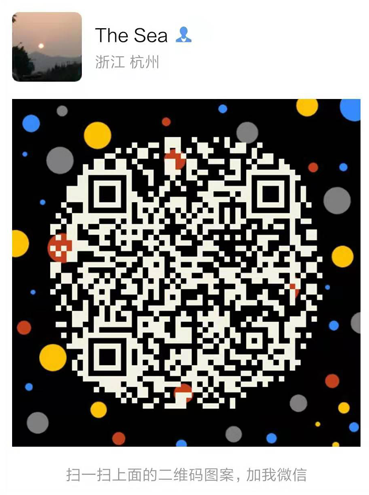
\includegraphics[scale=0.6]{example/leon.png}}
\centerline{\fontsize{26pt}{26pt} 微信}
\end{pre}
\pagestyle{empty}
\tableofcontents
\cleardoublepage
%# -*- coding: utf-8-unix -*-
\begin{overview}
\thispagestyle{empty}

为什么考研究僧,每个参与考试的人都有自己的想法。
~\\

相信,付出努力,就会有收获。

相信,当你觉得最迟的时候,恰恰是最早的时候。

相信,当你足够努力的时候,全世界都会为你让路。

相信,读书改变命运。

~\\

杭电,有人均两篇SCI的云计算实验室。

杭电,有人北大硕士MIT博士的顶级助教。

杭电,有数百块泰坦GPU构建的深度学习集群。

杭电,有对世界的抽象--图形图像实验室。

......
~\\

本人以题典的形式将杭电的题型抽象出来。
每道题都是对知识点的串接。学懂了每道题,也就对每个重要知识点的掌握。

\end{overview}

\mainmatter	  % 对正文用阿拉伯数字作为页码

%======================================================================
% 正文内容
\pagestyle{fancy}
\setcounter{page}{0}
%# -*- coding: utf-8-unix -*-
%%==================================================
\chapter{题典之Hash}
\label{chap1}
\begin{itemize}[noitemsep,topsep=0pt,parsep=0pt,partopsep=0pt]
	\item 知识点:讲解相关知识点。
	\item 题型:直接上真题。
\end{itemize}

\section{知识点和方法论}

\subsection{知识点}

\begin{itemize}[noitemsep,topsep=0pt,parsep=0pt,partopsep=0pt]
	\item 开放定址法:H(key)为题目选定的散列函数, m 列表长度, di为增量序列, Hi新的位置
	\begin{itemize}[noitemsep,topsep=0pt,parsep=0pt,partopsep=0pt]
		\item 核心公式:$$ Hi = (H(key) + di) \% m $$ 
		\item 线性探测法: $$ di=0,1,2,3,...,m-1 $$
		\item 平方探测法(又称二次探测): $$ di=0,1,-1,4,-4,... k^2, -k^2 (k <= m / 2)$$
	\end{itemize}
    \item 平均查找长度
    \begin{itemize}[noitemsep,topsep=0pt,parsep=0pt,partopsep=0pt]
    	\item $$ ASL_{\mbox{成功} } = (\mbox{查找成功的次数,第一次也算一次}) / \mbox{元素的个数} $$ 
    \end{itemize}
	\item 平均失败查找长度
	\begin{itemize}[noitemsep,topsep=0pt,parsep=0pt,partopsep=0pt]
		\item $$ ASL_{\mbox{失败}} = ({\color{red}\mbox{在mod数范围内的空间才算}})/ {\color{red}\mbox{MOD后面的数}} $$ 
	\end{itemize}
	\item 装填因子: 衡量冲突的概率
	\begin{itemize}[noitemsep,topsep=0pt,parsep=0pt,partopsep=0pt]
		\item $$ \alpha = n(\mbox{关键字个数}) / N (\mbox{表长}) $$ 
	\end{itemize}
	\item 链地址法
	\begin{itemize}[noitemsep,topsep=0pt,parsep=0pt,partopsep=0pt]
		\item 就像领接表那样
	\end{itemize}
\end{itemize}

\subsection{方法论}
\begin{enumerate}[noitemsep,topsep=0pt,parsep=0pt,partopsep=0pt]
	\item 画出数组
	\item 后面填入数字(比较次数)
\end{enumerate}

\section{真题实战}


\subsection{2017年第8题}


\begin{lstlisting}[basicstyle=\small\ttfamily, caption={2017年第8题}, numbers=none]
已知Hash函数为H(K) = K mod 13 ,散列地址为0--14,用开放地址发解决冲突,选取增量序列为线性探测再散列,关键字
23,34,56,24,75,12,59,52,36,92 依次插入到散列表中,则平均成功的查找长度为____ 、  平均失败的查找长度为 _____。
\end{lstlisting}


解:


\begin{tabular}{|c|c|c|c|c|c|c|c|c|c|c|c|c|c|c|}% 通过添加 | 来表示是否需要绘制竖线
	\hline  % 在表格最上方绘制横线
	0 & 1 & 2 & 3 & 4 & 5 & 6 & 7 & 8 & 9 & 10 & 11 & 12 & 13 & 14 \\
	\hline  %在第一行和第二行之间绘制横线
	52(1) & 36(7) & 92(2) &   & 56(1) &   &   &   & 34(1) &   & 23(1) & 24(1) & 75(3) & 12(2) & 49(5) \\
	\hline
	 4 & 3 & 2 &  1 & 2 & 1 &  1 &  1 & 2 & 1 & 9 & 8 & 7 & 6 &  5  \\
	\hline % 在表格最下方绘制横线
\end{tabular}




\begin{lstlisting}[basicstyle=\small\ttfamily, caption={}, numbers=none]
23 % 13 = 10
34 % 13 = 8   
56 % 13 = 4
24 % 13 = 11
75 % 13 = 10  冲突  (10 + 1 ) % 15=11 冲突 (10 + 2)% 15 = 12
12 % 13 = 12  冲突  (12 + 1) % 15 =13 
49 % 13 = 10  冲突   (10 + 1 ) % 15=11 冲突 (10 + 2)% 15 = 12 冲突 (10 + 3) % 15 =13 冲突  (10 + 4) % 15 = 14
52 % 13 = 0 
36 % 13 = 10  冲突   (10 + 1 ) % 15=11 冲突 (10 + 2)% 15 = 12 冲突 (10 + 3) % 15 =13 冲突  (10 + 4) % 15 = 14 (10 + 5) % 15 = 0 冲突(10 + 6)% 15 = 1 
92 % 13 = 1 (1+1)% 15 = 2
\end{lstlisting}

\rule[-10pt]{20cm}{0.05em}

\begin{flalign}
1 + 7 + 2 + 1 + 1 + 1+ 1 + 3 + 2 + 5 &= 24  (\mbox{查找次数}) &&\\
24 / 10 &=2.4  (\mbox{平均查找长度}) 
\end{flalign}


对于0地址的元素要查找0,1,2,3这几个元素才知道会不会失败,第三个是空元素,所以失败了
对于1地址的元素要查找1,2,3这几个元素才知道会不会失败,第3个元素是空元素,所以失败了
以此类推
因为 mod 13 只用看  0 - 12空间里面的错误 
\begin{flalign}
(4+ 3 + 2 + 1 + 2 + 1 + 1 +1 + 2 + 1 + 9 + 8 + 7 ) &= 42 &&\\ 
ASL_{\mbox{失败}} &= 42 / 13 
\end{flalign}



\subsection{王道269综合应用题第3题}
\begin{figure}[htbp]
	\centering  % 环境中的内容居中排版
	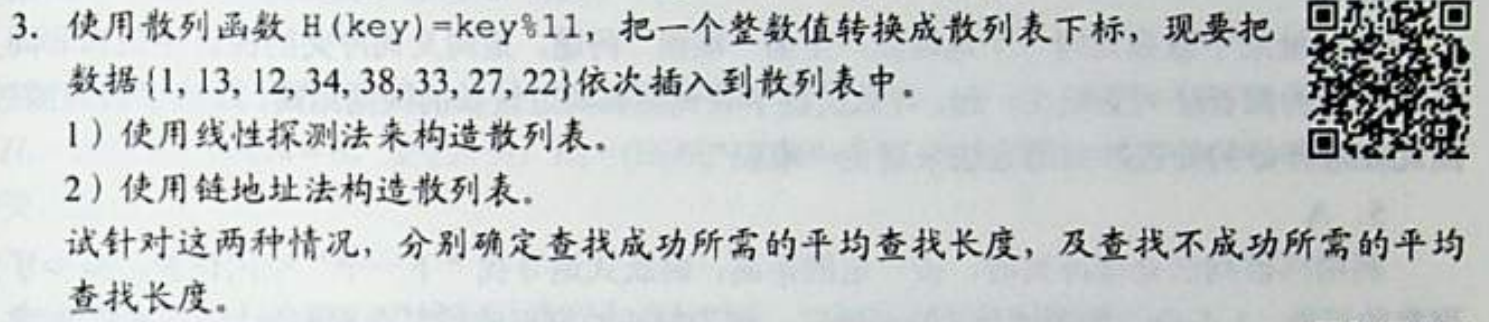
\includegraphics[scale=0.3]{example/chapter1/wangdao269_3.png}
	\caption{王道269综合应用题第3题}
\end{figure}


解:

1)
~\\
\begin{center}
\begin{tabular}{|c|c|c|c|c|c|c|c|c|c|c|}% 通过添加 | 来表示是否需要绘制竖线
	\hline  % 在表格最上方绘制横线
	0 & 1 & 2 & 3 & 4 & 5 & 6 & 7 & 8 & 9 & 10\\
	\hline  %在第一行和第二行之间绘制横线
	33(1) & 1(1) & 13(1) & 12(3) & 34(4) & 38(1)  & 27(2) & 22(8)  &  &   &  \\
	\hline % 在表格最下方绘制横线
\end{tabular}
\end{center}
~\\

\begin{lstlisting}[basicstyle=\small\ttfamily, caption={}, numbers=none]
1 % 11 = 1 
13 % 11 = 2
12 % 11 = 1冲突   (1+1)% 10 = 2 冲突   (1  + 2) % 10 = 3
34 % 11 = 1冲突   (1+1)% 10 = 2 冲突   (1  + 2) % 10 = 3 冲突(1+ 3) % 10 = 4 
33 % 11 = 0
38 % 11 = 5
27 % 11 = 5 冲突 (5+1)%10 = 6
22 % 11 = 0 冲突  1 冲突 2 冲突3 冲突4 冲突5 冲突 6冲突   7
\end{lstlisting}
~\\
2)
\\~
拉链法只要算一次
\begin{lstlisting}[basicstyle=\small\ttfamily, caption={}, numbers=none]
1 % 11 = 1 
13 % 11 = 2
12 % 11 = 1
34 % 11 = 1 
33 % 11 = 0
38 % 11 = 5
27 % 11 = 5 
22 % 11 = 0 
\end{lstlisting}

\begin{figure}[H]
	\centering  % 环境中的内容居中排版
	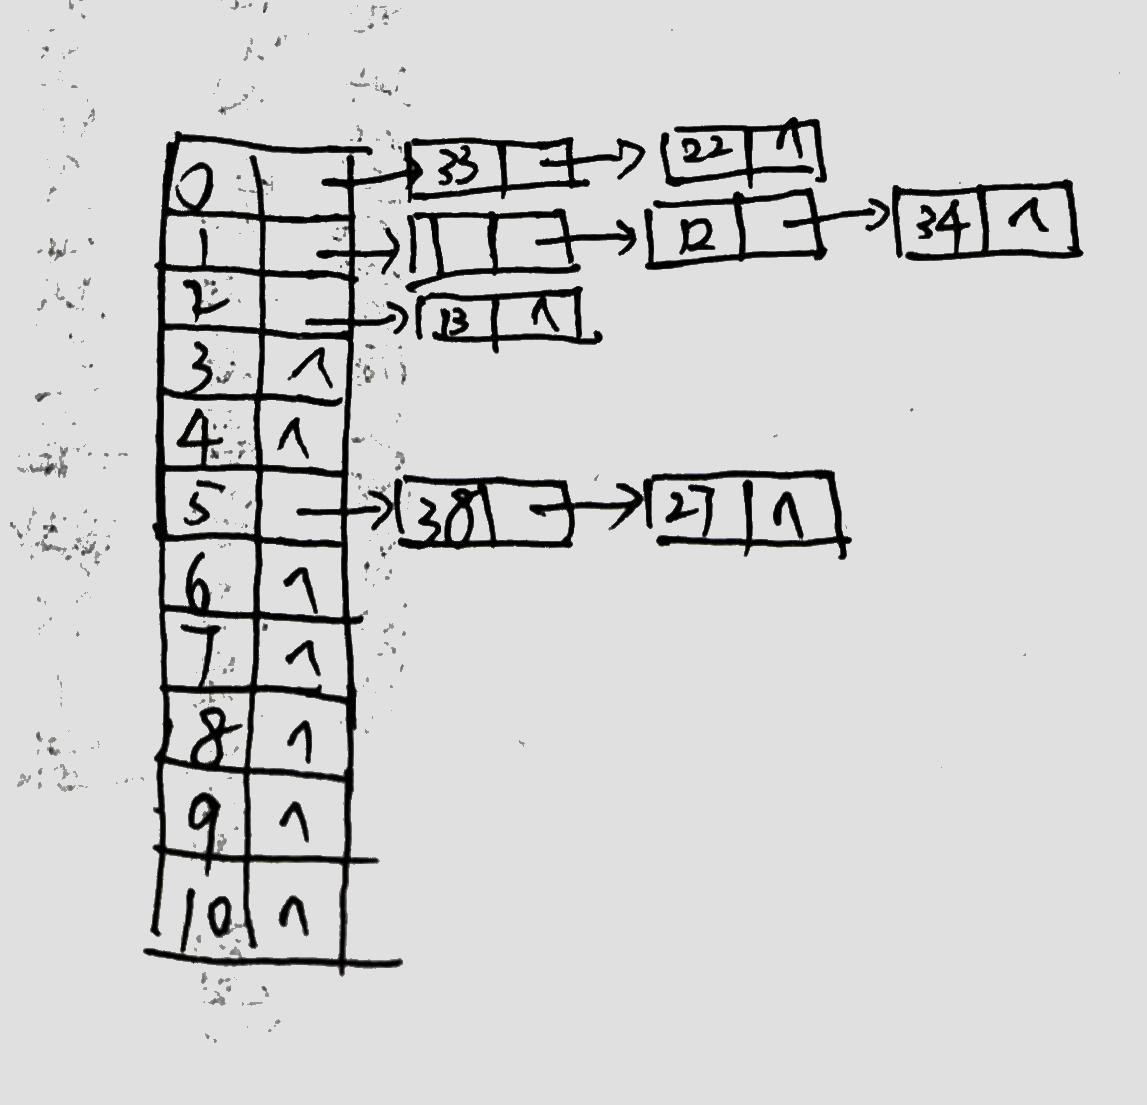
\includegraphics[scale=0.3]{example/chapter1/lalianfa.jpg}
	\caption{王道269综合应用题第3题}
\end{figure}

3)
\\~
\begin{lstlisting}[basicstyle=\small\ttfamily, caption={}, numbers=none]
用A B 指代 1) 2)
A
A(ASL 成功) = (1+ 1 + 1 + 3 + 4 + 1 + 2 + 8)/8=21 / 8
A(ASL 失败) = (9 + 8 + 7 + 6 + 5 + 4 + 3 + 2 + 1 + 1 + 1) / 11 = 47 / 11
B
B(ASL成功) = (4*1 + 3*2 + 3 * 1)/8 = 13 / 8
B(ASL失败) = (3 + 4 + 2 + 1 + 1 + 3 + 1*5) / 11 = 19 / 11
\end{lstlisting}


\subsection{2015年第(5)题}


\begin{lstlisting}[basicstyle=\small\ttfamily, caption={}, numbers=none]
设散列函数 H(K) = 3K mod 11, 散列地址空间为 0 - 10, 对关键字序列 (32,13,39,24,38,21,4,12) 按照下述两种解决冲突的方法构造散列表;
1) 线性探测再散列;
2) 链地址法;
3) 并分别求出等概率下查找成功时和查找失败时的平均查找长度 ASL_{succ} 和 ASL_{UNSUCC};
\end{lstlisting}
解:
\\~
\begin{center}
\begin{tabular}{|c|c|c|c|c|c|c|c|c|c|c|}% 通过添加 | 来表示是否需要绘制竖线
	\hline  % 在表格最上方绘制横线
	0 & 1 & 2 & 3 & 4 & 5 & 6 & 7 & 8 & 9 & 10\\
	\hline  %在第一行和第二行之间绘制横线
	& 4(1) &   & 49(1) & 38(1) & 12(3)  & 13(1) & 24(2)  & 32(1) & 21(2)  &   \\
	\hline % 在表格最下方绘制横线
\end{tabular}
\end{center}

\begin{lstlisting}[basicstyle=\small\ttfamily, caption={}, numbers=none]
(3*32) % 11 = 8
(13*3) % 11 = 6   
(49*3) % 11 = 3
(24*3) % 11 = 6 冲突 (6+1) %11 = 7
(38*3) % 11 = 4
(21*3) % 11 = 8 冲突 (8+1) %11 = 9
(4*3)  % 11 = 1
(12*3) % 11 = 3 冲突  4 冲突  5
\end{lstlisting}
~\\
\begin{flalign}
ASL_{\mbox{失败}} &= (1+2+8+7+6+5+4+3+2+1) / 11 =  39/11 &&\\ 
ASL_{\mbox{成功}} &= (1+1+1+3+1+2+1+2) / 8 = 1.5
\end{flalign}
\\~
\begin{flalign}
ASL_{\mbox{失败}} &= (1+2+1+3+2+1+3+1+3+1+1) / 11 =  19/11 &&\\ 
ASL_{\mbox{成功}} &= (5*1 + 3*2) / 8 = 11 / 8 
\end{flalign}


\subsection{2013年第4题}


\begin{lstlisting}[basicstyle=\small\ttfamily, caption={}, numbers=none]
设哈希函数为H(key) = key mod 13 哈希表长为15,用开放定址法处理冲突,增量序列使用二次探测再散列。若一次在哈希表中插入11个元素:
34,12,67,43,98,23,51,86,05,37,22
1) 画出他们在表中的分布情形。
2) 求其等概率情况下平均成功的查找长度
\end{lstlisting}

解:

\begin{center}
\begin{tabular}{|c|c|c|c|c|c|c|c|c|c|c|c|c|c|c|}% 通过添加 | 来表示是否需要绘制竖线
	\hline  % 在表格最上方绘制横线
	0 & 1 & 2 & 3 & 4 & 5 & 6 & 7 & 8 & 9 & 10 & 11 & 12 & 13 & 14 \\
	\hline  %在第一行和第二行之间绘制横线
	&  & 67(1) & 22(6) & 43(1) & 5(1)  &   &  98(1) & 34(1) & 86(2)  & 23(1) & 37(1) & 12(1) & 51(2) &  \\
	\hline % 在表格最下方绘制横线
\end{tabular}
\end{center}
~\\
\begin{lstlisting}[basicstyle=\small\ttfamily, caption={}, numbers=none]
39 % 13 = 8
12 % 13 = 12
67 % 13 = 2
43 % 13 = 4
98 % 13 = 7
23 % 13 = 10
51 % 13 = 12 冲突 (12+1) % 15 = 13
86 % 13 = 8 冲突 (8+1) % 15 = 9
5 % 13 =5
37 % 13 = 11
22 % 13 = 9 冲突 (9+1) %15 = 10 冲突 (9-1)%15 = 8 冲突 (9+4) %15 = 13 冲突 (9-4) %15 = 5 冲突 (9+9) %15 = 3
\end{lstlisting}
~\\
\begin{flalign}
ASL_{\mbox{成功}} &= (1+6+1=1+1+1+2+1+1+1+2) / 11 = 18/11
\end{flalign}


\subsection{2014年第4题}
\begin{lstlisting}[basicstyle=\small\ttfamily, caption={}, numbers=none]
采用哈希后函数H(k) = 3*k mod 13 并用开放地址发处理冲突,增量序列选取采用线性探测再散列方式,在数列地址空间[0..12]中对关键字序列
22,41,53,46,30,13,1,67,51
1) 构造哈希表(画示意图);
2) 装填因子;
3) 查找成功时的平均查找长度;
4) 查找不成功时的平均查找长度。
\end{lstlisting}
解:
~\\
\begin{center}
\begin{tabular}{|c|c|c|c|c|c|c|c|c|c|c|c|c|}% 通过添加 | 来表示是否需要绘制竖线
	\hline  % 在表格最上方绘制横线
	0 & 1 & 2 & 3 & 4 & 5 & 6 & 7 & 8 & 9 & 10 & 11 & 12  \\
	\hline  %在第一行和第二行之间绘制横线
	13,1& 66,1 &  & 53,1 & 1,2 &   & 41,1  &  67,2 & 46,1 &   & 51,1 &  & 30,1   \\
	\hline % 在表格最下方绘制横线
\end{tabular}
\end{center}
~\\
\begin{lstlisting}[basicstyle=\small\ttfamily, caption={}, numbers=none]
3*22 % 13 = 1
41*3 % 13 = 6
53*3 % 13 = 3
46*3 % 13 = 8
30*3 % 13 = 12
13*3 % 13 = 0
(1*3)% 13 = 3 冲突 4
(667*3)%13 = 6 冲突 7
(51*3) %13 = 10
\end{lstlisting}
~\\
\begin{flalign}
\alpha = \frac{n}{N} = \frac{9}{13}
\end{flalign}
~\\
\begin{flalign}
ASL_{\mbox{成功}} &= (1+1+1+2+1+2+1+1+1) / 9 = 11/9 &&\\
ASL_{\mbox{失败}} &= (3+2+1+3+2+1+4+3+2+1+2+1+4) / 13 = 29/13 
\end{flalign}



 % hash
%%# -*- coding: utf-8-unix -*-
%%==================================================

\chapter{树和二叉树}
\label{chap2}

\begin{itemize}[noitemsep,topsep=0pt,parsep=0pt,partopsep=0pt]
	\item 知识点:讲解相关知识点。
	\item 题型:直接上真题。
\end{itemize}

\section{知识点和方法论}

\subsection{知识点}
\begin{itemize}[noitemsep,topsep=0pt,parsep=0pt,partopsep=0pt]
	\item 树和森林的遍历与二叉树遍历的对应关系
	~\\
	\begin{center}
	\begin{tabular}{|c|c|c|}% 通过添加 | 来表示是否需要绘制竖线
		\hline  % 在表格最上方绘制横线
		先根遍历 & 先序遍历 & 先序遍历 \\
		\hline  %在第一行和第二行之间绘制横线
		后根遍历 & 中序遍历 & 中序遍历 \\
		\hline % 在表格最下方绘制横线
	\end{tabular}
	\end{center}
	\item 树的高度(深度)是从1开始计算的
	\item 公式$总结点数 = 总分支数 + 1   ==>  N2 + N1 + N0 = N1 + 2*N2 + 1$
	\item 完全二叉树的公式(二叉树的节点序号从1开始) $ 当 i \le \lfloor n/2 \rfloor $ 则节点i为分支节点,否则为叶子节点。
	\item 层次遍历二叉树,BFS,DFS的应用。
	\item 并查集的应用 参考链接 \url{https://blog.csdn.net/liuyang981122/article/details/81530014} 杭电复试笔试 \url{https://blog.csdn.net/weixin_42044546/article/details/88876958}
	\item 树的结点个数 = 树的边数+1
\end{itemize}
\begin{lstlisting}[basicstyle=\small\ttfamily, caption={}, numbers=none]
Staus InOrderTrav(BiTree T,Status(* Visit)(TElemType e)){
	//中序遍历二叉树T的非递归算法,对每个数据元素调用函数visit.
	InitStack(S);  Push(S,T);    //根指针进栈
	while(!StackEmpty(S)){
		while((GetTop(S,p)&&p)  Push(S,p->lchild);//p赋值转换,向左走到尽头
		Pop(S,p);  //空指针退栈
		if(!StackEmpty(S)){   //访问结点,向右一步
			Pop(S,p); if(!Visit(p->data)) return error;
			Push(S,p->rchild);
		} //if
	} //while
	Return ok;
} //InOrderTraverse
\end{lstlisting}

\subsection{方法论}
\begin{enumerate}[noitemsep,topsep=0pt,parsep=0pt,partopsep=0pt]
\item 把树和森林转化为二叉树处理
\item 对应看
\item 画出森林
\begin{itemize}[noitemsep,topsep=0pt,parsep=0pt,partopsep=0pt]
\item 首先画出二叉树
\item 把二叉树的右子树断开,变为树
\item 把右子树移动一定的角度 然后再断开兄弟节点,然后连接双亲节点
\end{itemize}
	 首先画出二叉树
	 把二叉树的右子树断开,变为树
	 把右子树移动一定的角度 然后再断开兄弟节点,然后连接双亲节点
\item 表示方法
\begin{itemize}[noitemsep,topsep=0pt,parsep=0pt,partopsep=0pt]
	\item 孩子兄弟表示法
	\item 孩子表示法像邻接表那样的
\end{itemize}

\item 森林表示为二叉树
\begin{itemize}[noitemsep,topsep=0pt,parsep=0pt,partopsep=0pt]
	\item 先把兄弟链断开
	\item 依次作为右子树的节点
\end{itemize}

\item 二叉树的中序线索化
\begin{itemize}[noitemsep,topsep=0pt,parsep=0pt,partopsep=0pt]
	\item 写出中序的序列然后根据中序的序列画上图片,哪一个是先,哪一个是后一目了然
\end{itemize}

\end{enumerate}


\section{真题实战}


\subsection{2017年第1题}


\begin{lstlisting}[basicstyle=\small\ttfamily, caption={}, numbers=none]
已知二叉树的现需,中序,后续遍历的结果分别如下,请 
1) 画出这个二叉树
2) 补齐遍历中的空白处
3) 画出中序线索化二叉树形。
先序序列 : _B_F_ICEH_G
中序序列 : D_KFIA_EJCG
后序序列 : DKIF_HJEGCA
\end{lstlisting}

解:
\begin{lstlisting}[basicstyle=\small\ttfamily, caption={}, numbers=none]
易知
DLR ABDFKICEHJG
LDR DBKFIAHEJCG
LRD DKIFBHJEGCA
\end{lstlisting}

\begin{figure}[H]
	\centering  % 环境中的内容居中排版
	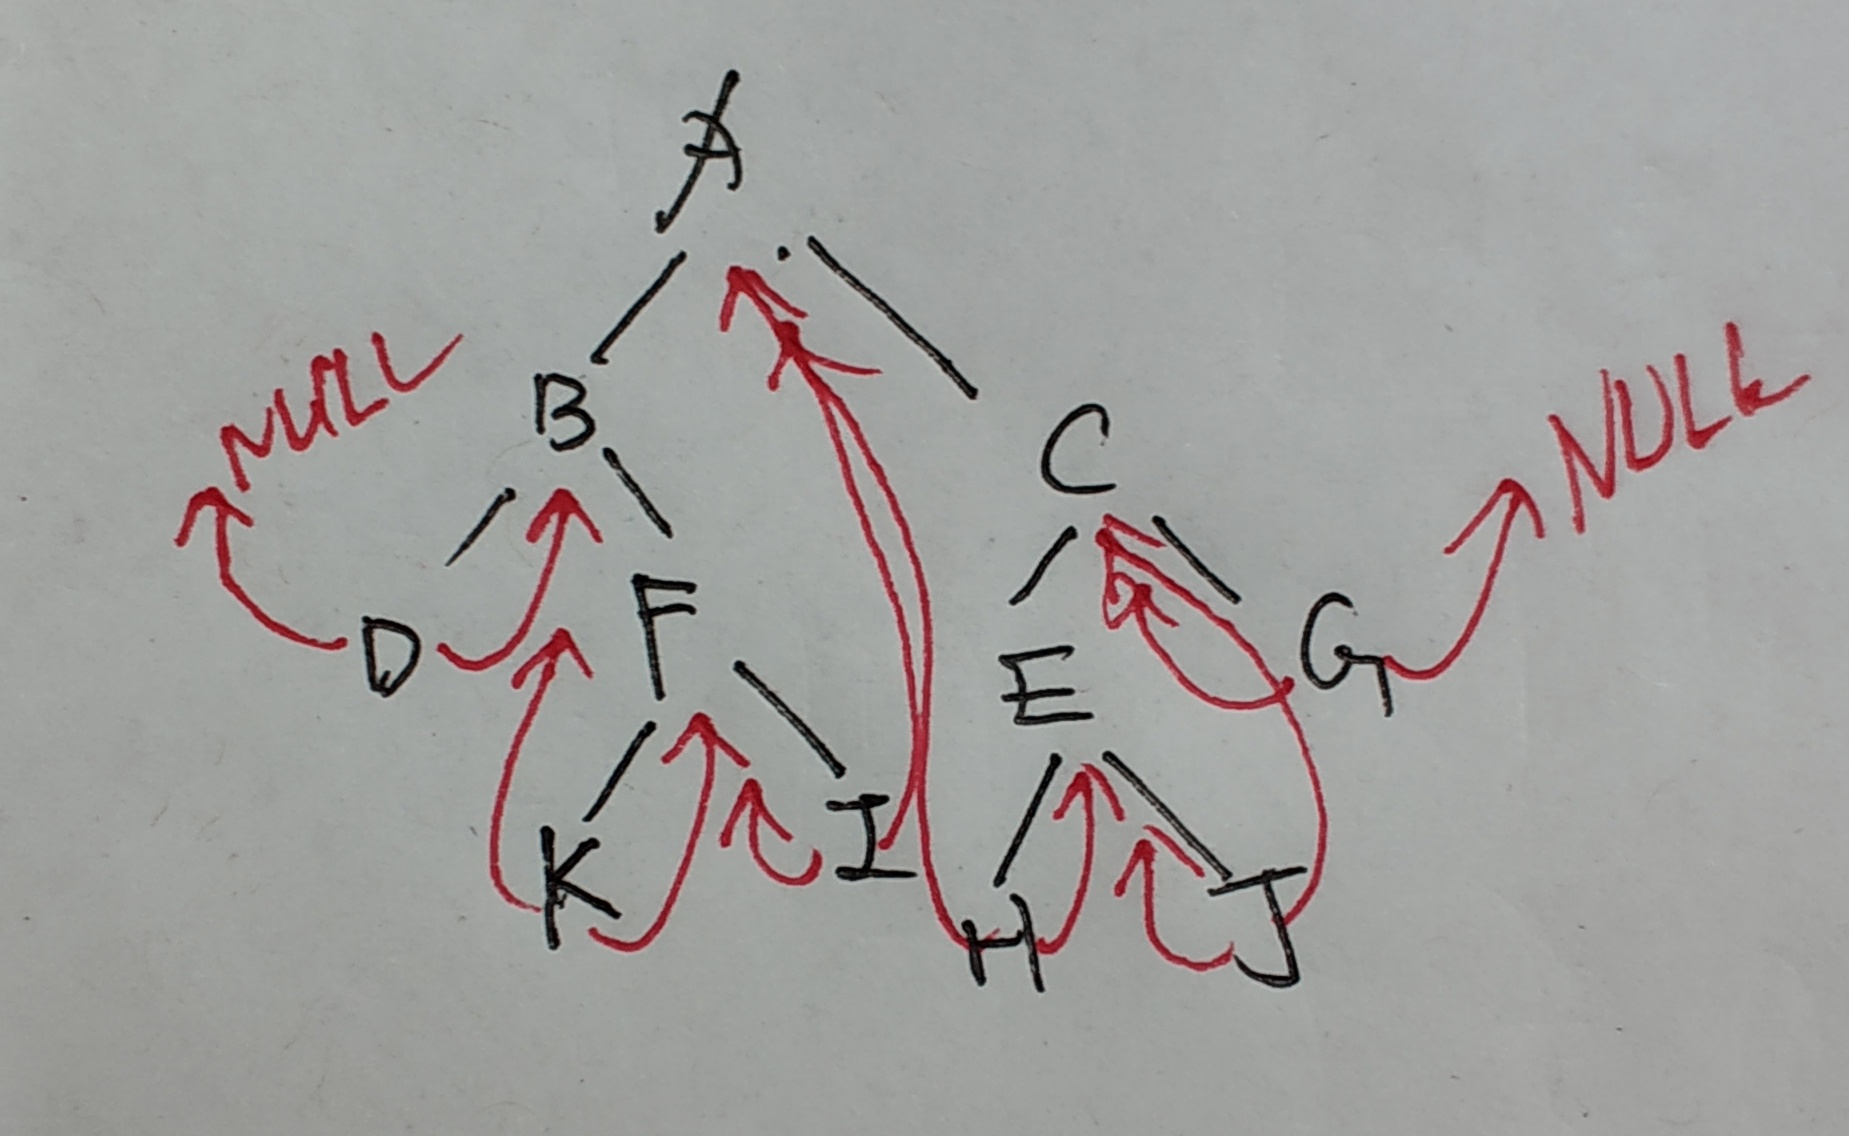
\includegraphics[scale=0.3]{example/chapter2/bitree20171.png}
\end{figure}


\subsection{2014年第3题}


\begin{figure}[H]
	\centering  % 环境中的内容居中排版
	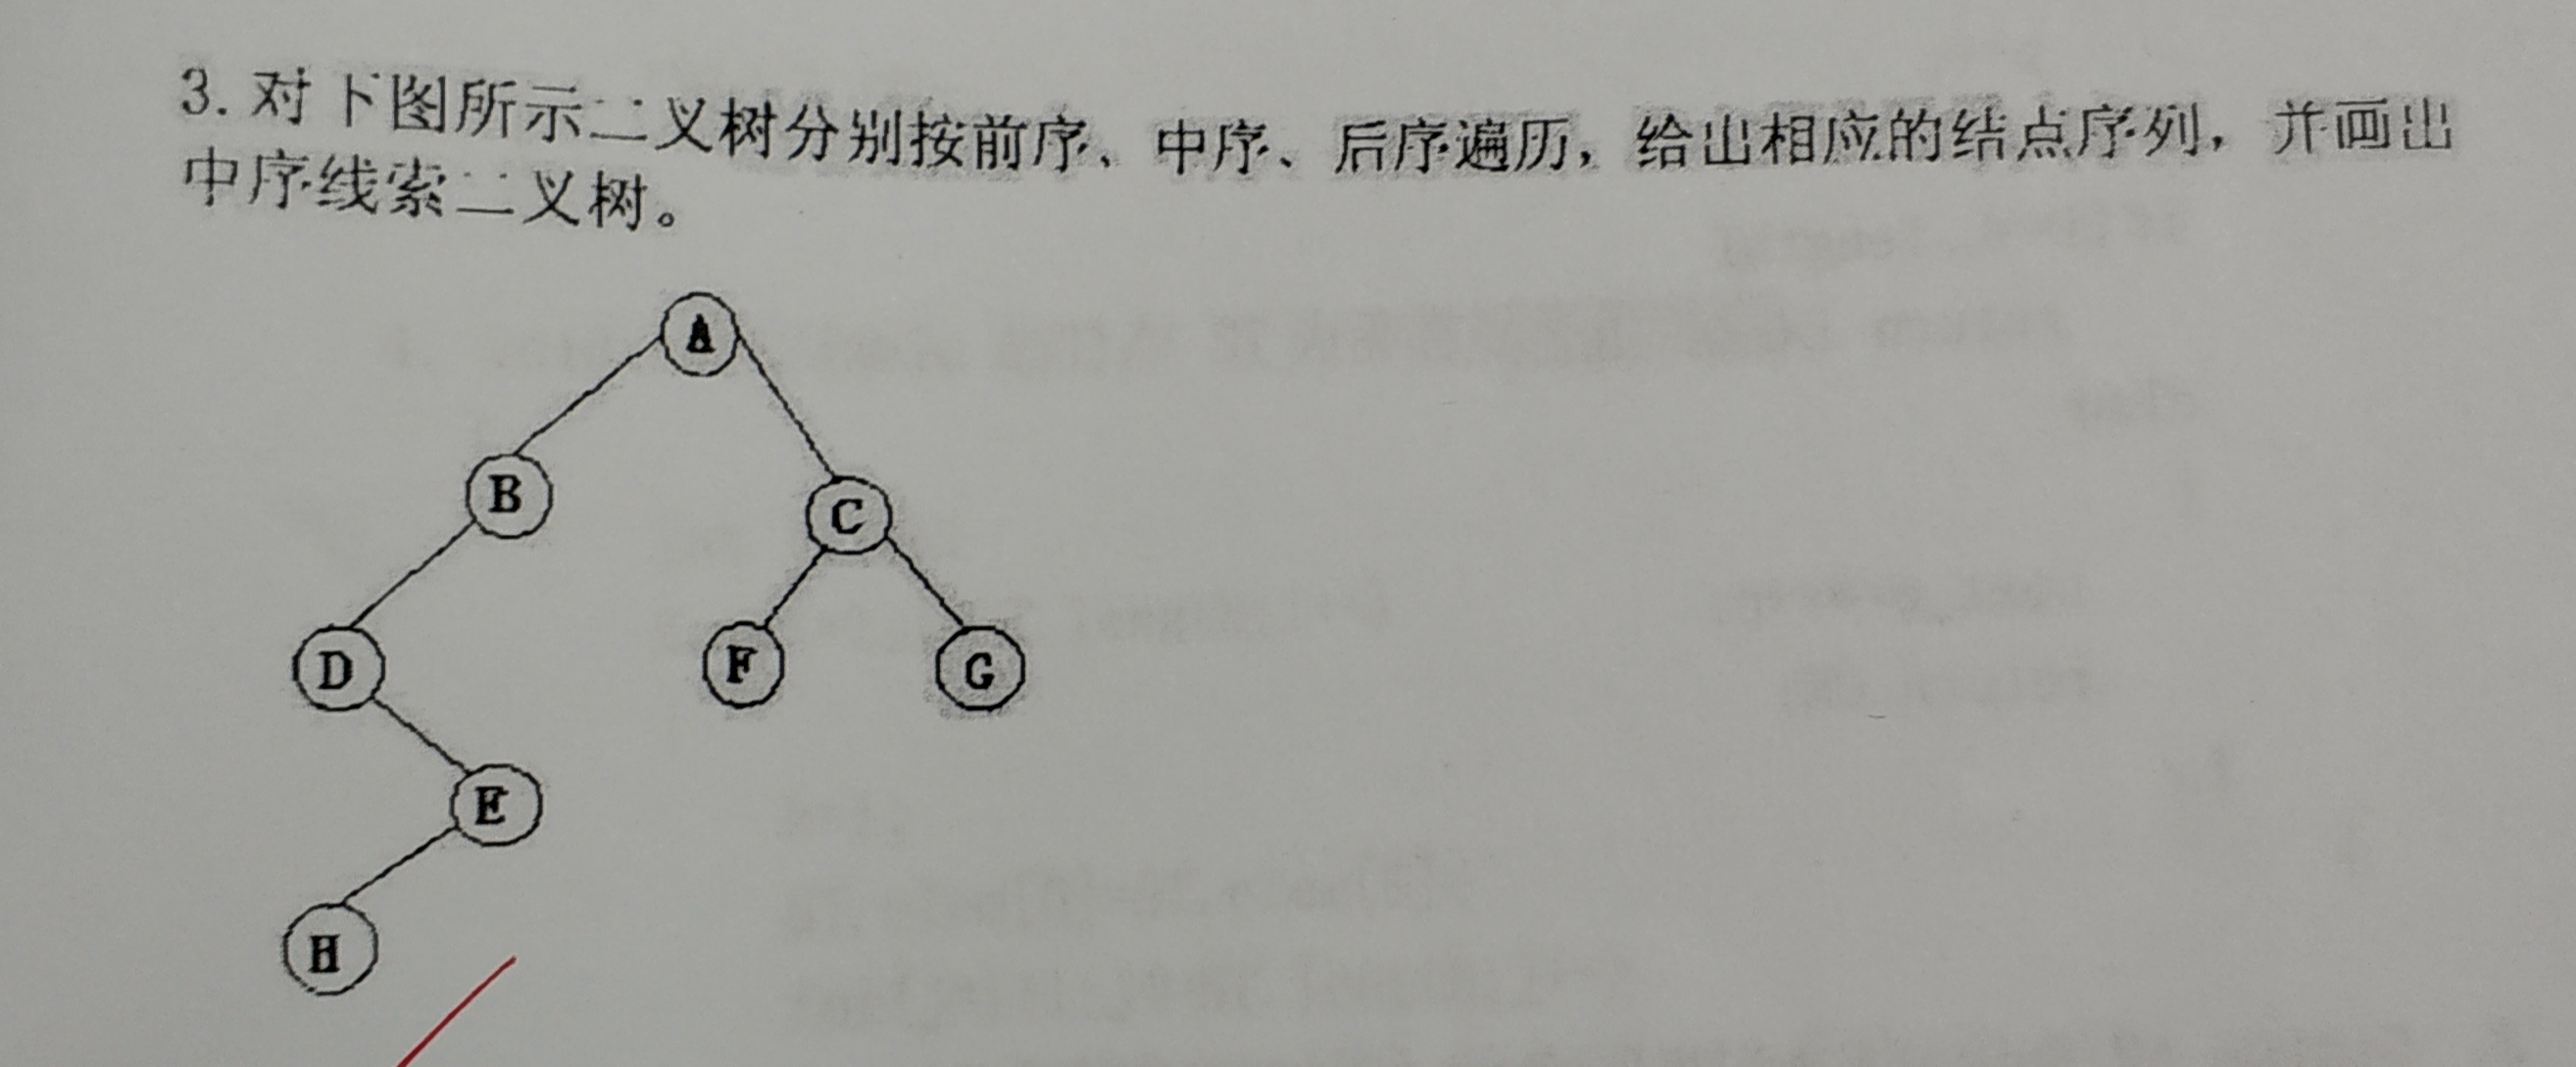
\includegraphics[scale=0.3]{example/chapter2/bitree20143.png}
\end{figure}

解:

\begin{lstlisting}[basicstyle=\small\ttfamily, caption={}, numbers=none]
易知
DLR  A B D E H C F G
LDR  D H E B A F C G
LRD  H E D B F G C A
\end{lstlisting}

\begin{figure}[H]
	\centering  % 环境中的内容居中排版
	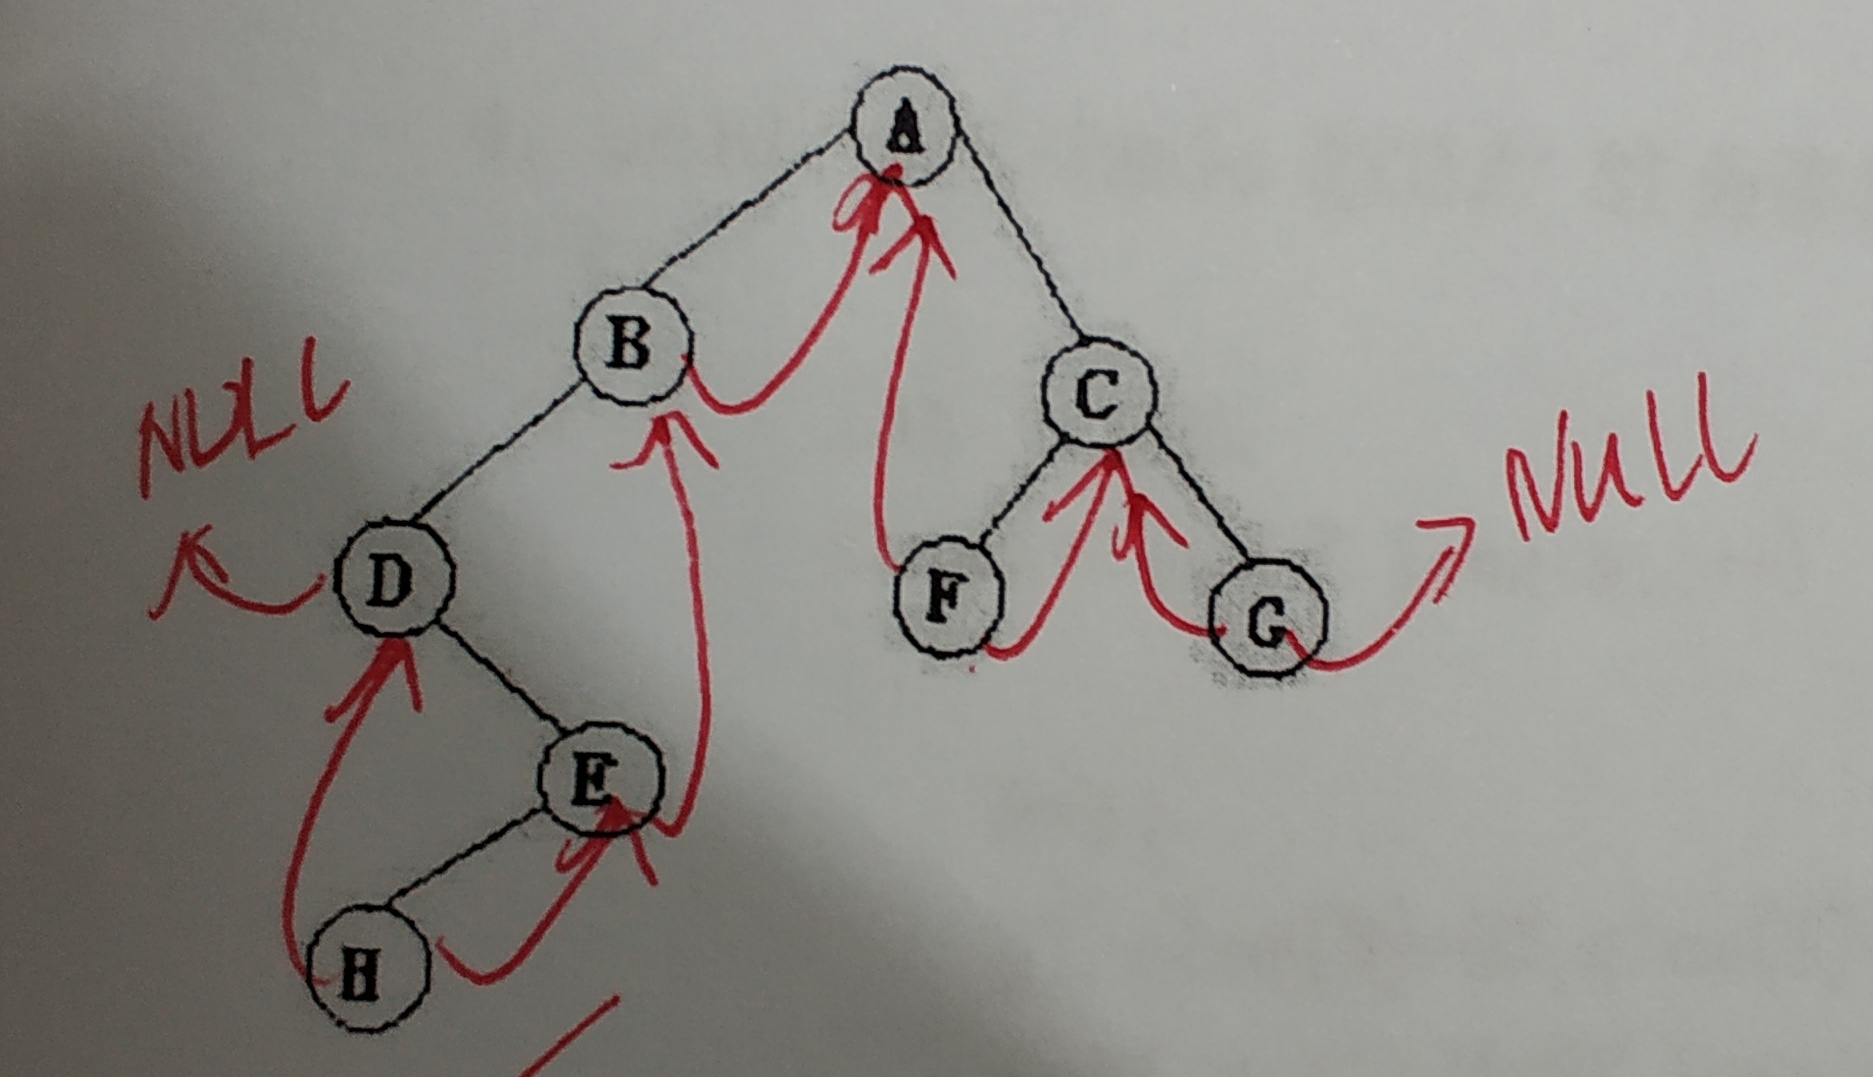
\includegraphics[scale=0.3]{example/chapter2/bitree20143ans.png}
\end{figure}


\subsection{2014年第一题}

\begin{lstlisting}[basicstyle=\small\ttfamily, caption={}, numbers=none]
已知某森林的先序遍历次序为:A,D,E,F,G,H,B,I,C,J,K,L,M,N,
中序遍历次序为:D,F,G,H,E,A,I,B,J,L,M,N,K,C
1) 画出该森林
2) 画出该森林用孩子兄弟法表示的存储结构
\end{lstlisting}
~\\
1)
~\\
详细解析\newline
DLR: {\color{red}A}{\color{blue}DEFGH}BICJKLMN\newline
LDR: {\color{blue}DFGHE}{\color{red}A}IBJLMNKC\newline
先看DLR中A表示的root节点,左边和右边分为左子树和右子树\newline
细化如果只剩下这两个\newline
DLR: {\color{blue}D}EFGH\newline
LDR: {\color{blue}D}FGHE\newline
说明D是root节点且没有左子树\newline
DLR:{\color{blue}E}FGH\newline
LDR:FGH{\color{blue}E}\newline
说明 E 是root节点且没有右子树\newline
DLR:F G H\newline
LDR:F G H\newline
他们顺序相同表示的是只有右子树的序列\newline
以此类推\newline
\begin{figure}[H]
	\centering  % 环境中的内容居中排版
	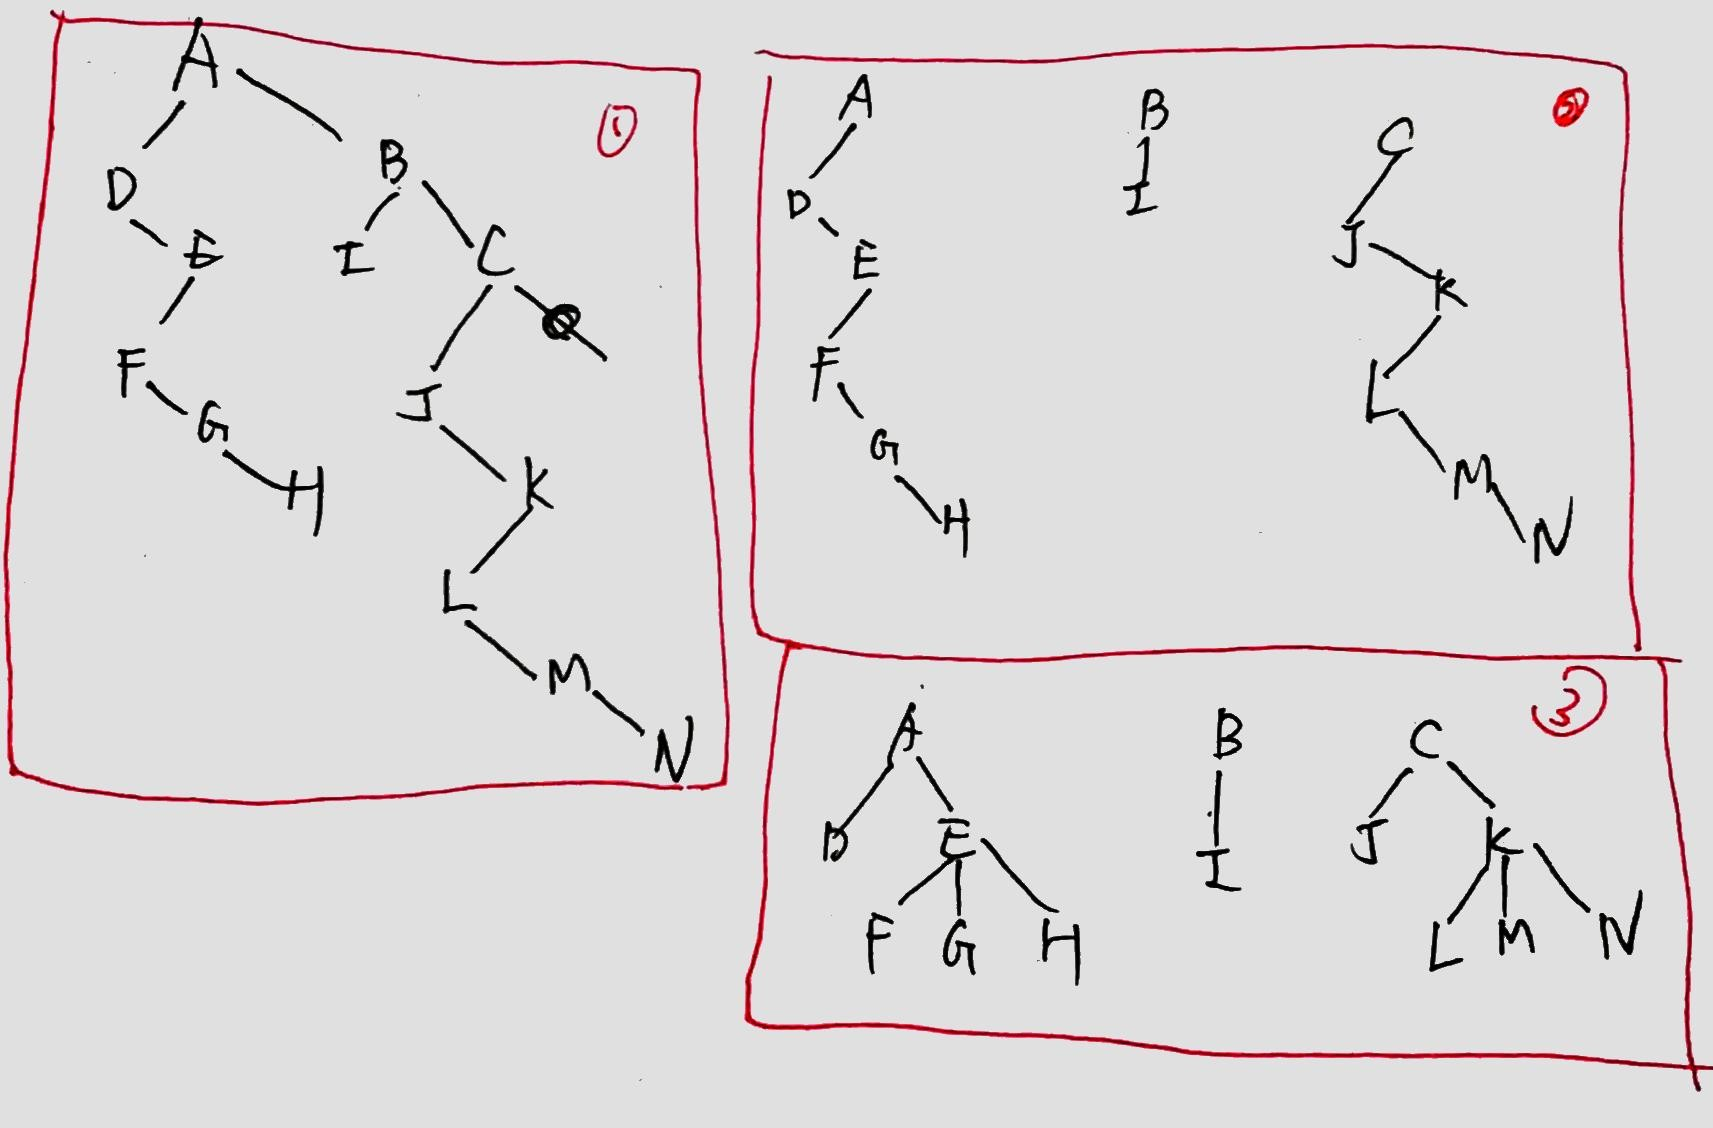
\includegraphics[scale=0.3]{example/chapter2/Img_181127155705826-1.jpg}
\end{figure}
~\\
2)
~\\
因为是孩子兄弟表示法所以存储结构是

\begin{figure}[H]
	\centering  % 环境中的内容居中排版
	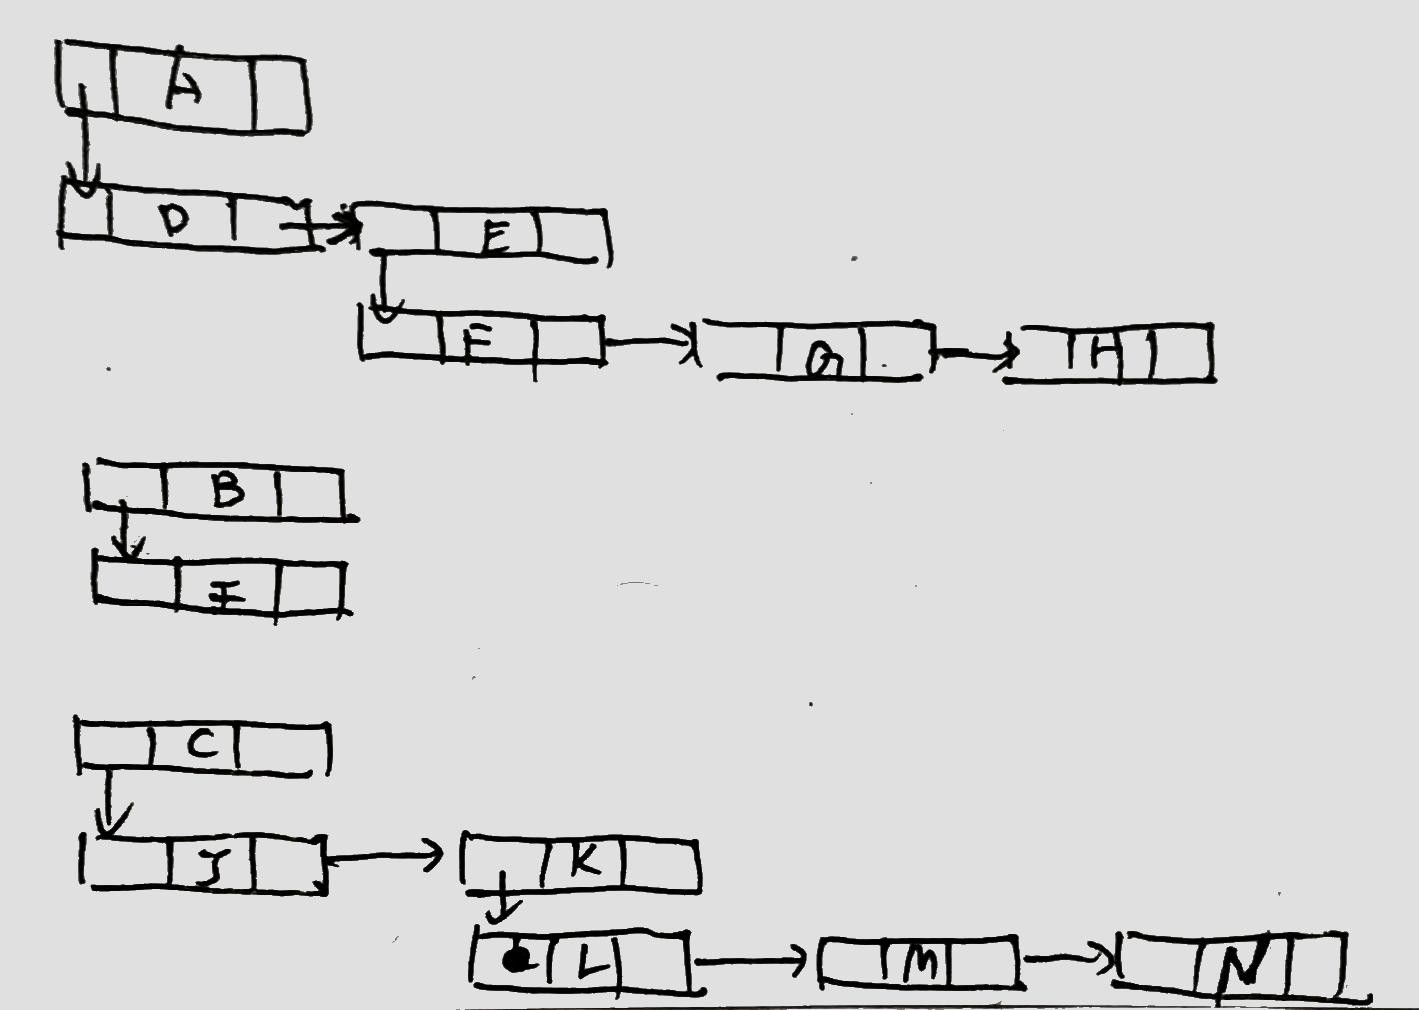
\includegraphics[scale=0.3]{example/chapter2/Img_181127161017119-1.jpg}
\end{figure}

\subsection{2015(1)}

\begin{figure}[H]
	\centering  % 环境中的内容居中排版
	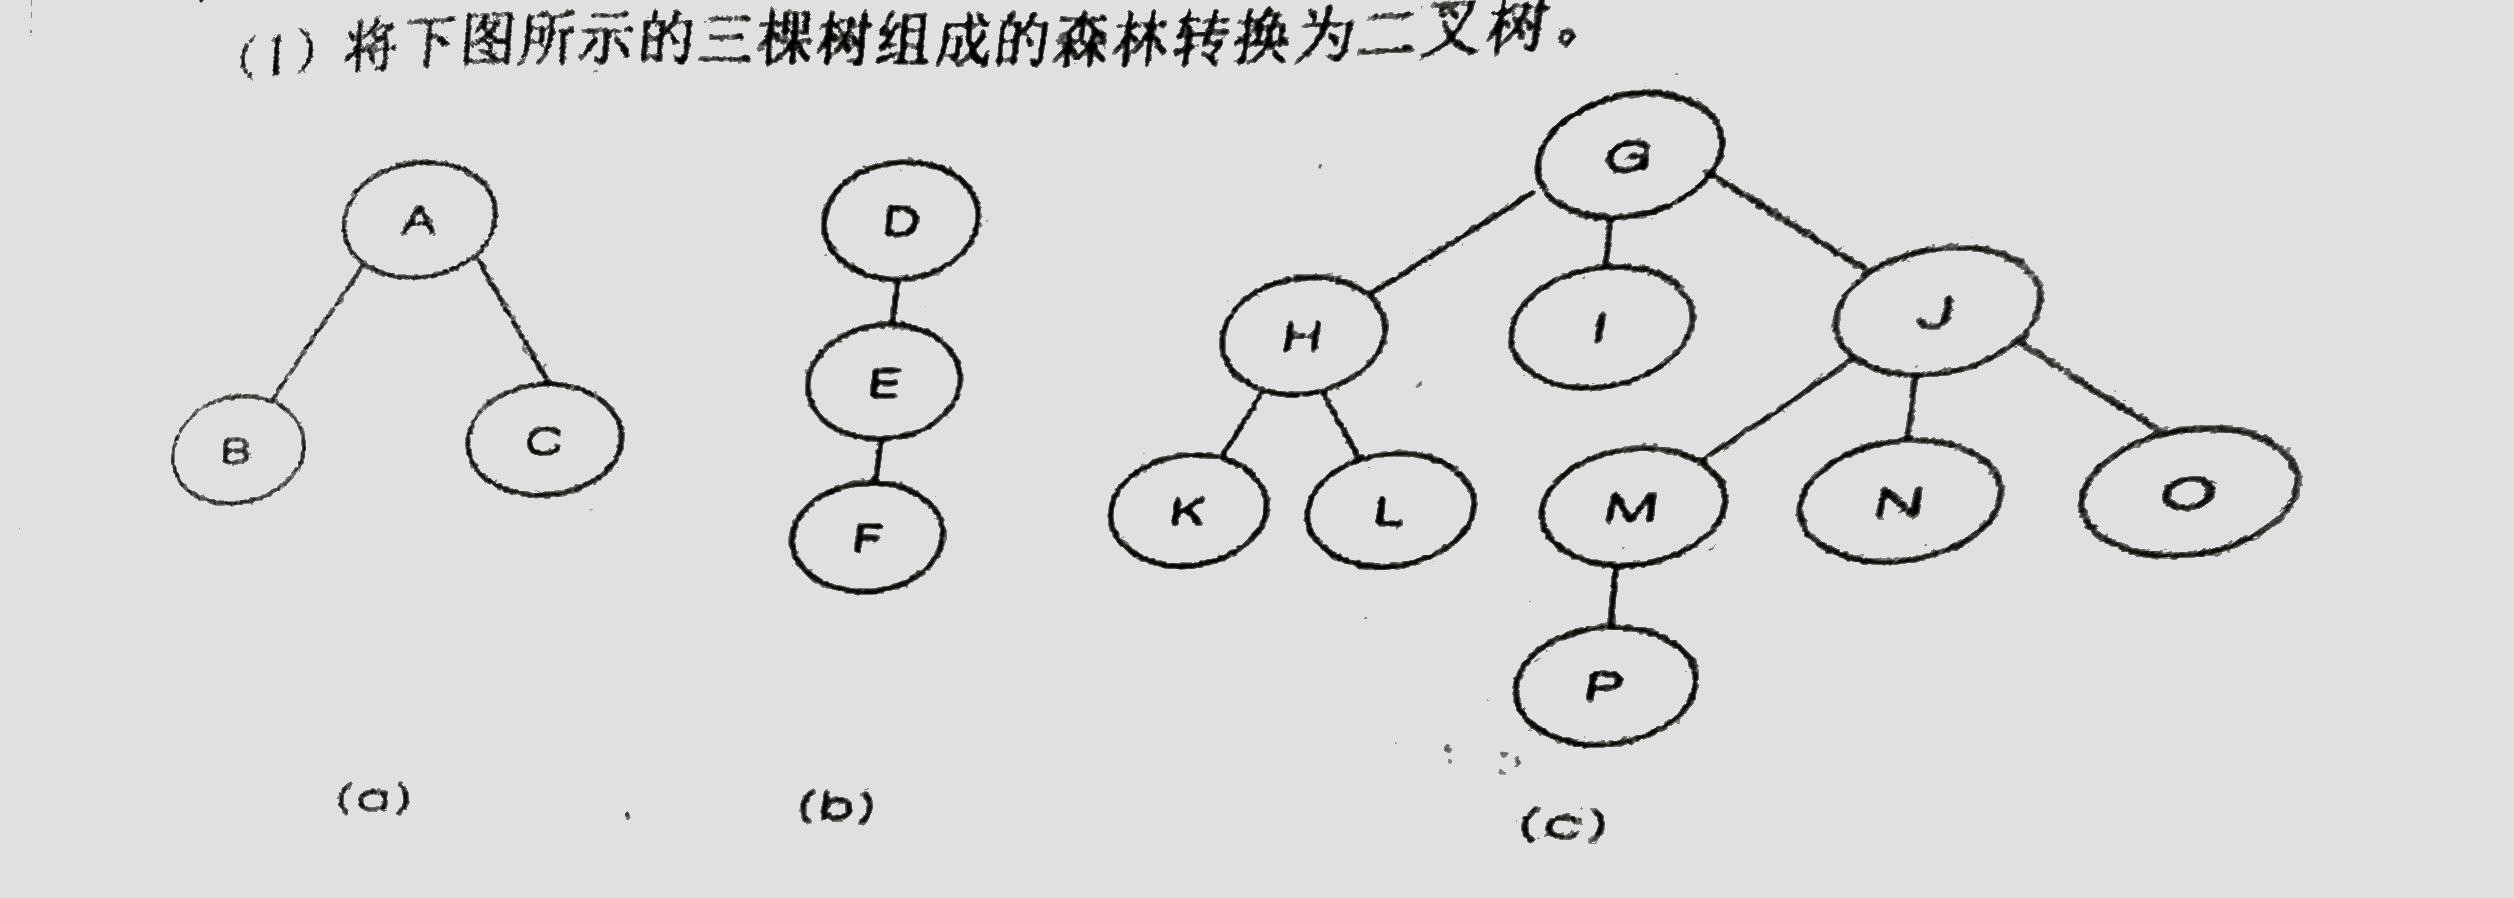
\includegraphics[scale=0.3]{example/chapter2/Img_181127161553384-1.jpg}
\end{figure}

解:

\begin{figure}[H]
	\centering  % 环境中的内容居中排版
	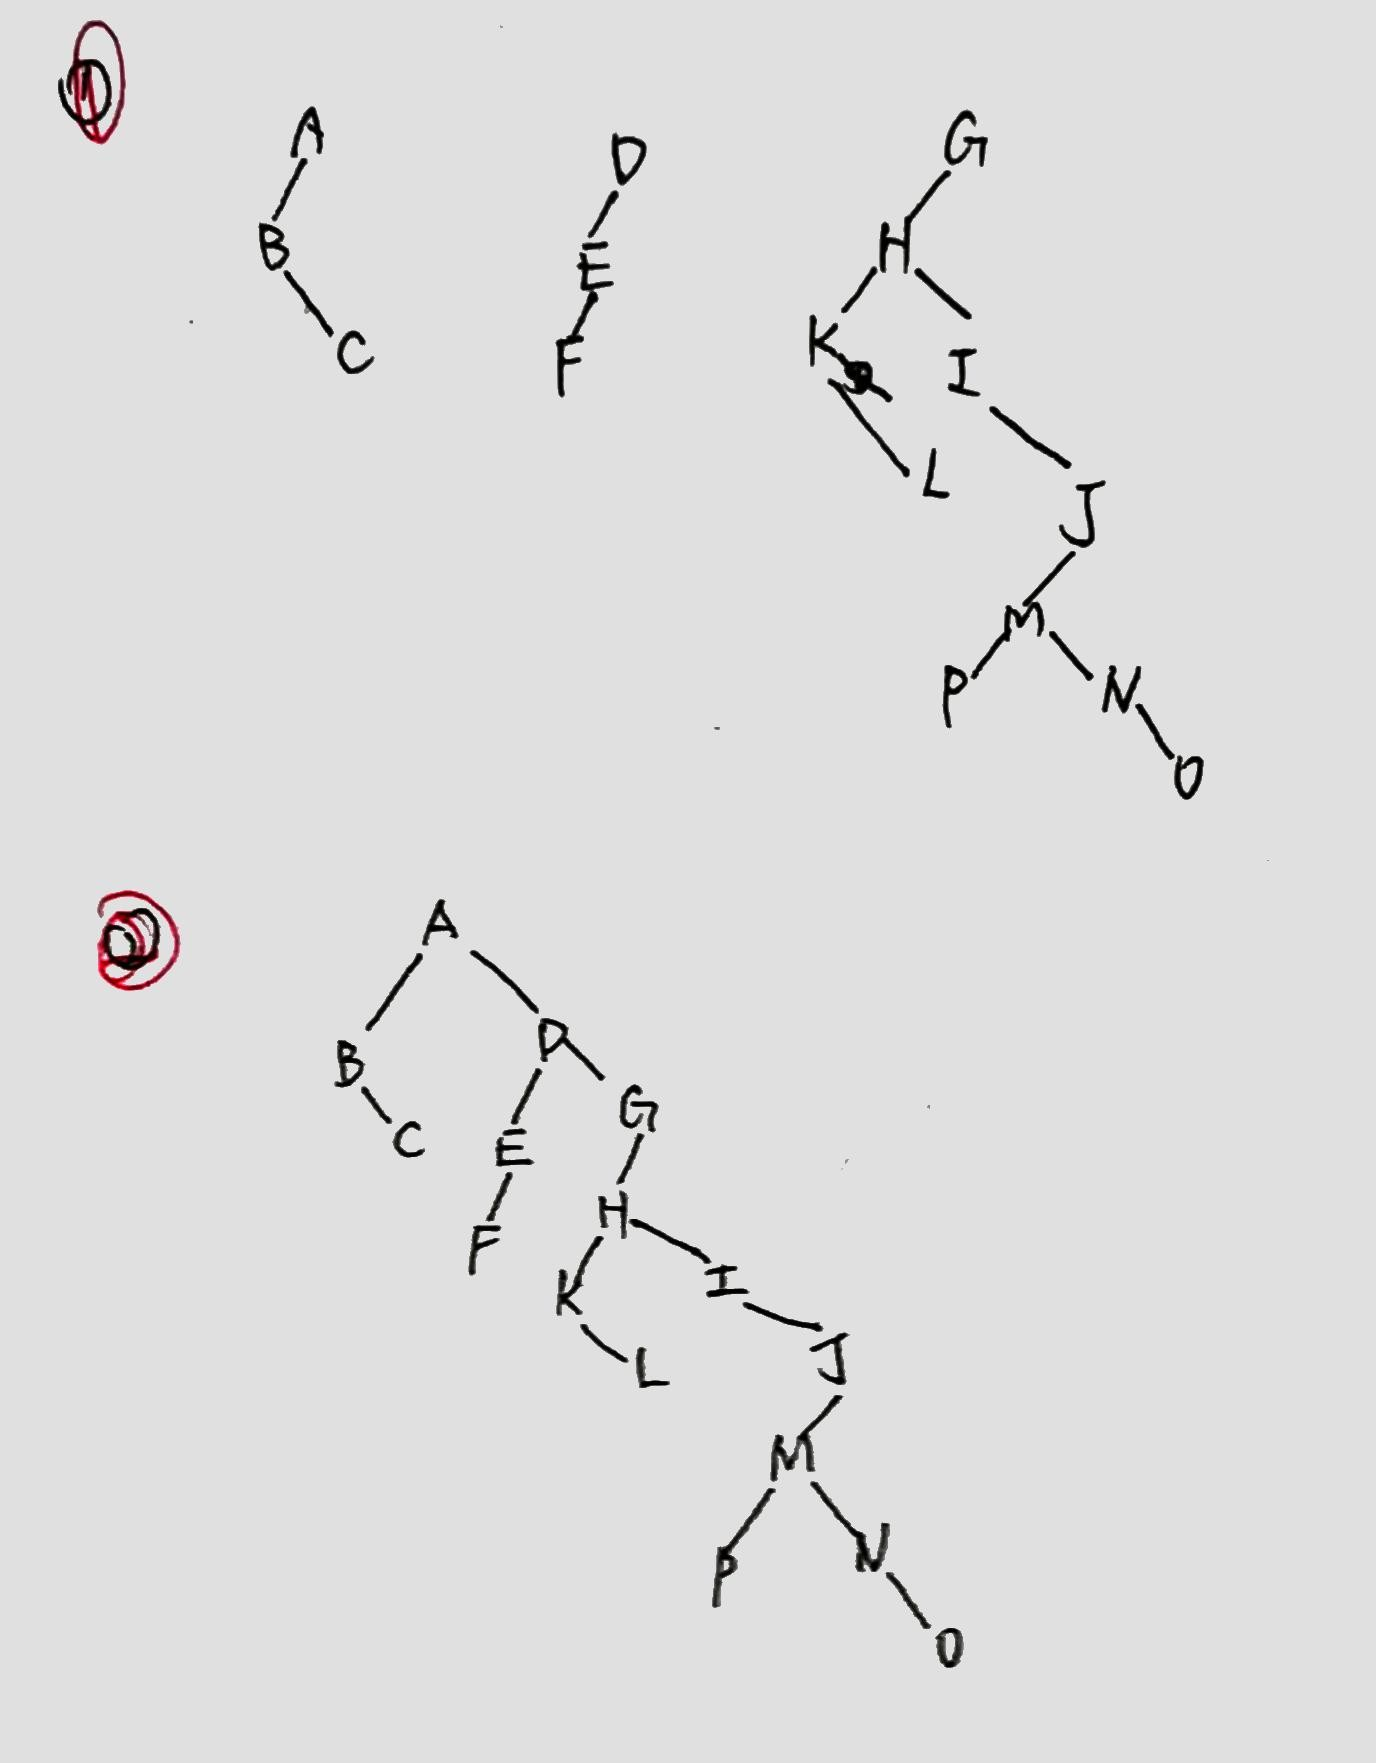
\includegraphics[scale=0.3]{example/chapter2/Img_181127161929409-1.jpg}
\end{figure}


\subsection{2016(2)}

\begin{figure}[H]
	\centering  % 环境中的内容居中排版
	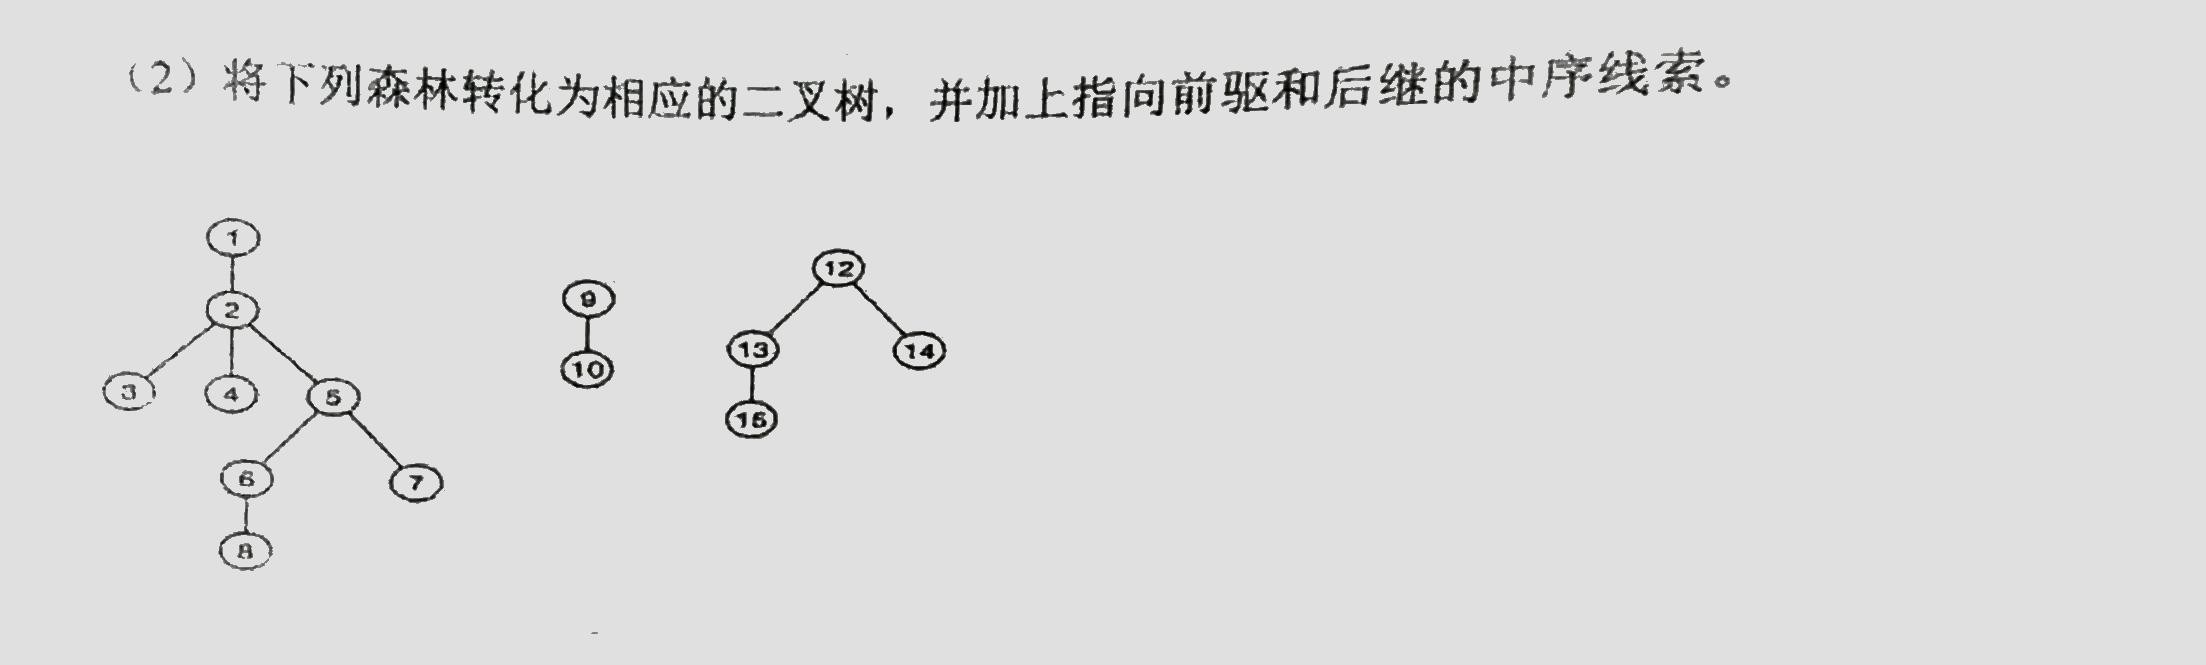
\includegraphics[scale=0.3]{example/chapter2/Img_181127162304566-1.jpg}
\end{figure}

解:

\begin{figure}[H]
	\centering  % 环境中的内容居中排版
	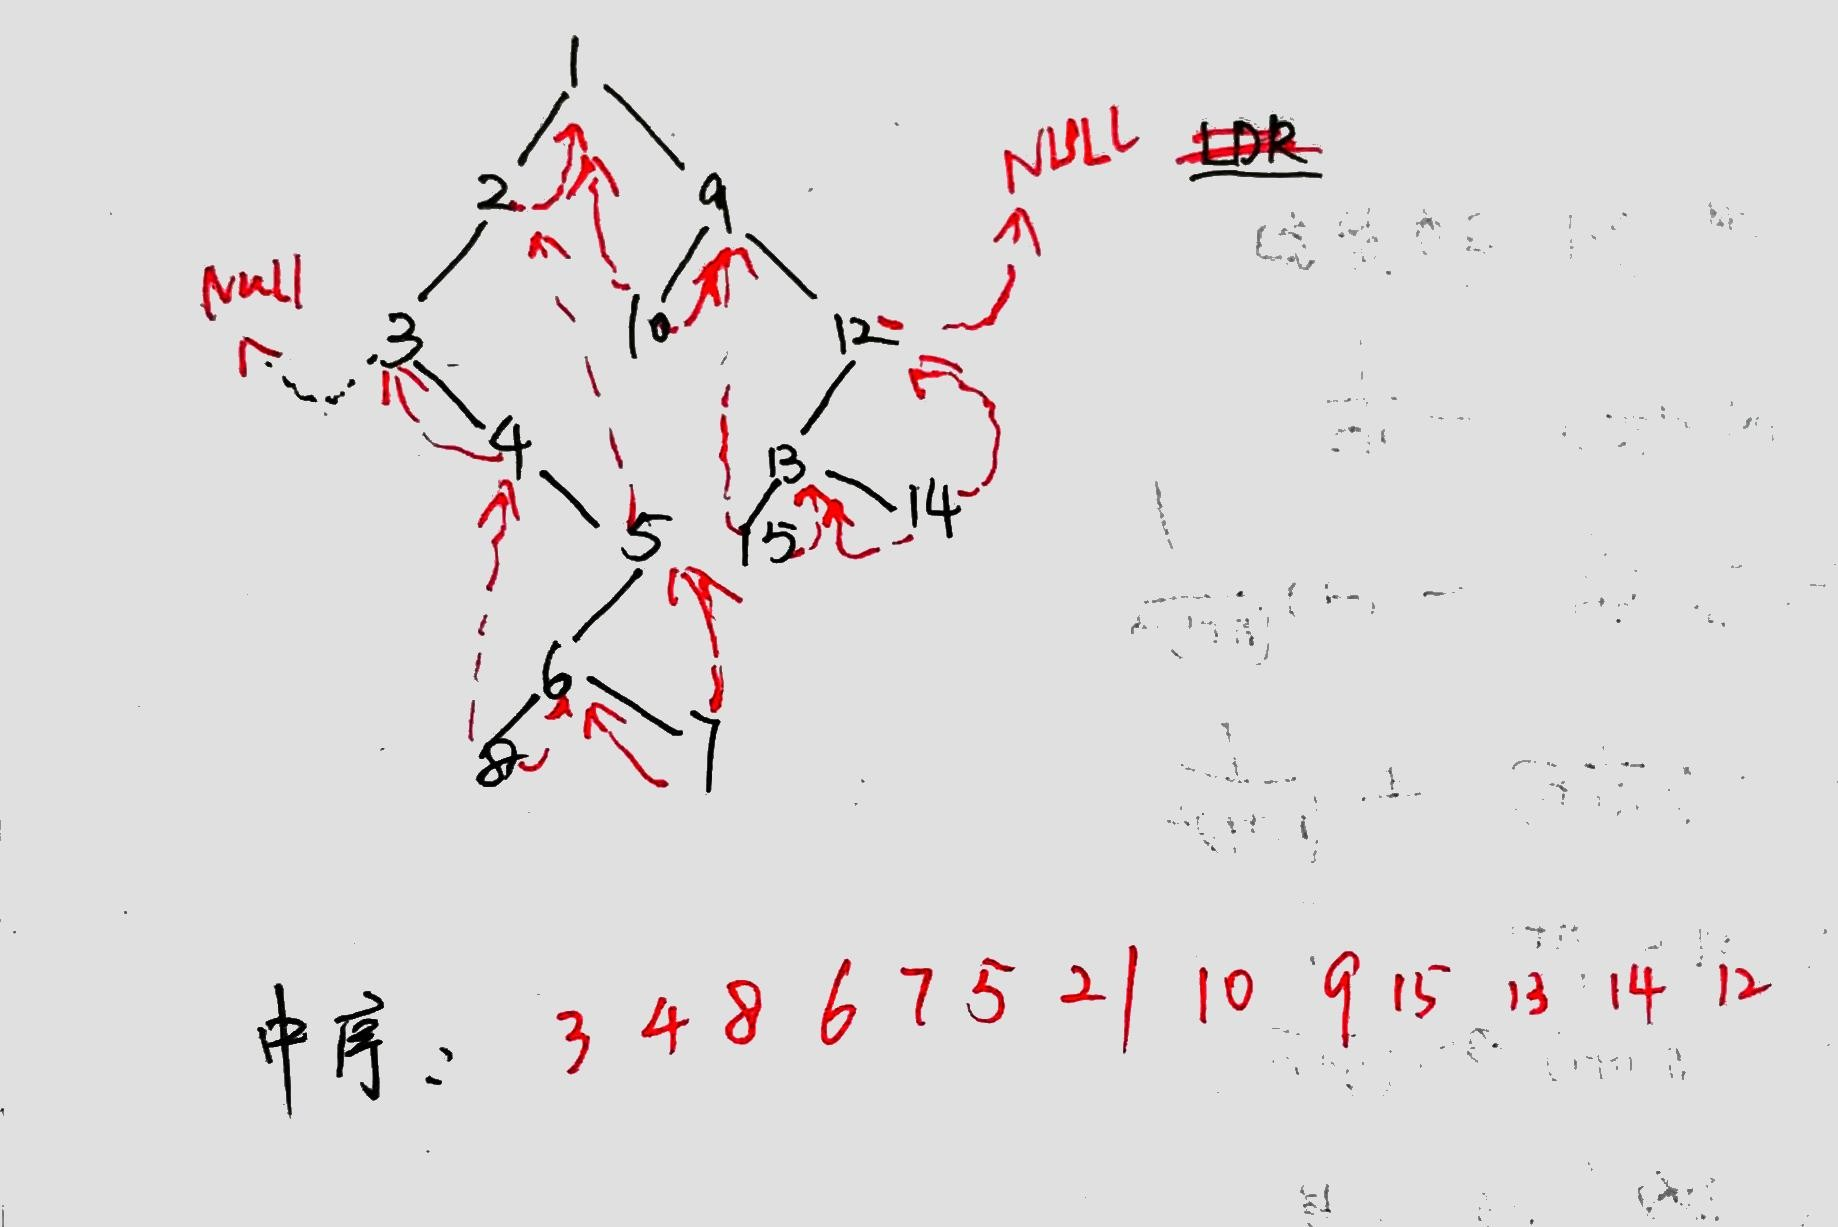
\includegraphics[scale=0.3]{example/chapter2/Img_181127163657518-1.jpg}
\end{figure}

\subsection{2017(2)}

\begin{figure}[H]
	\centering  % 环境中的内容居中排版
	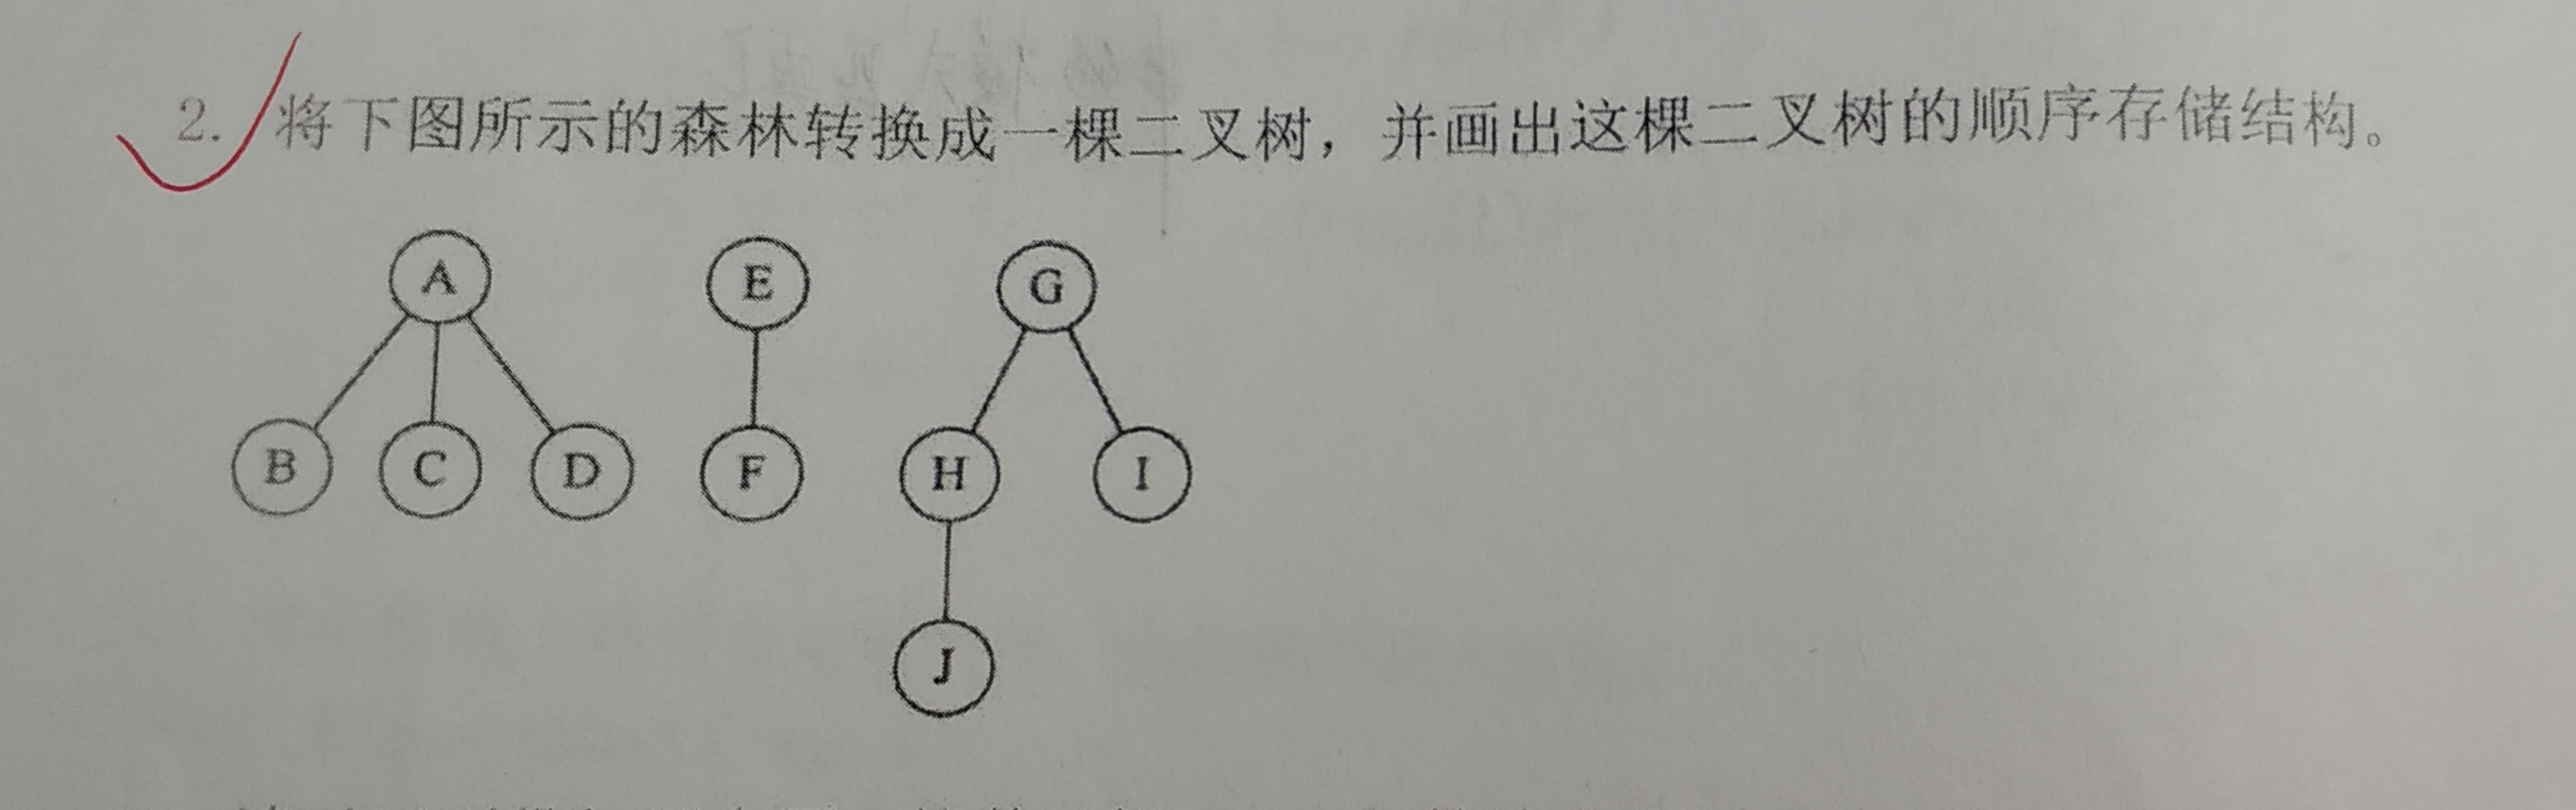
\includegraphics[scale=0.1]{example/chapter2/IMG_20181127_164746.png}
\end{figure}

解:


\begin{figure}[H]
	\centering  % 环境中的内容居中排版
	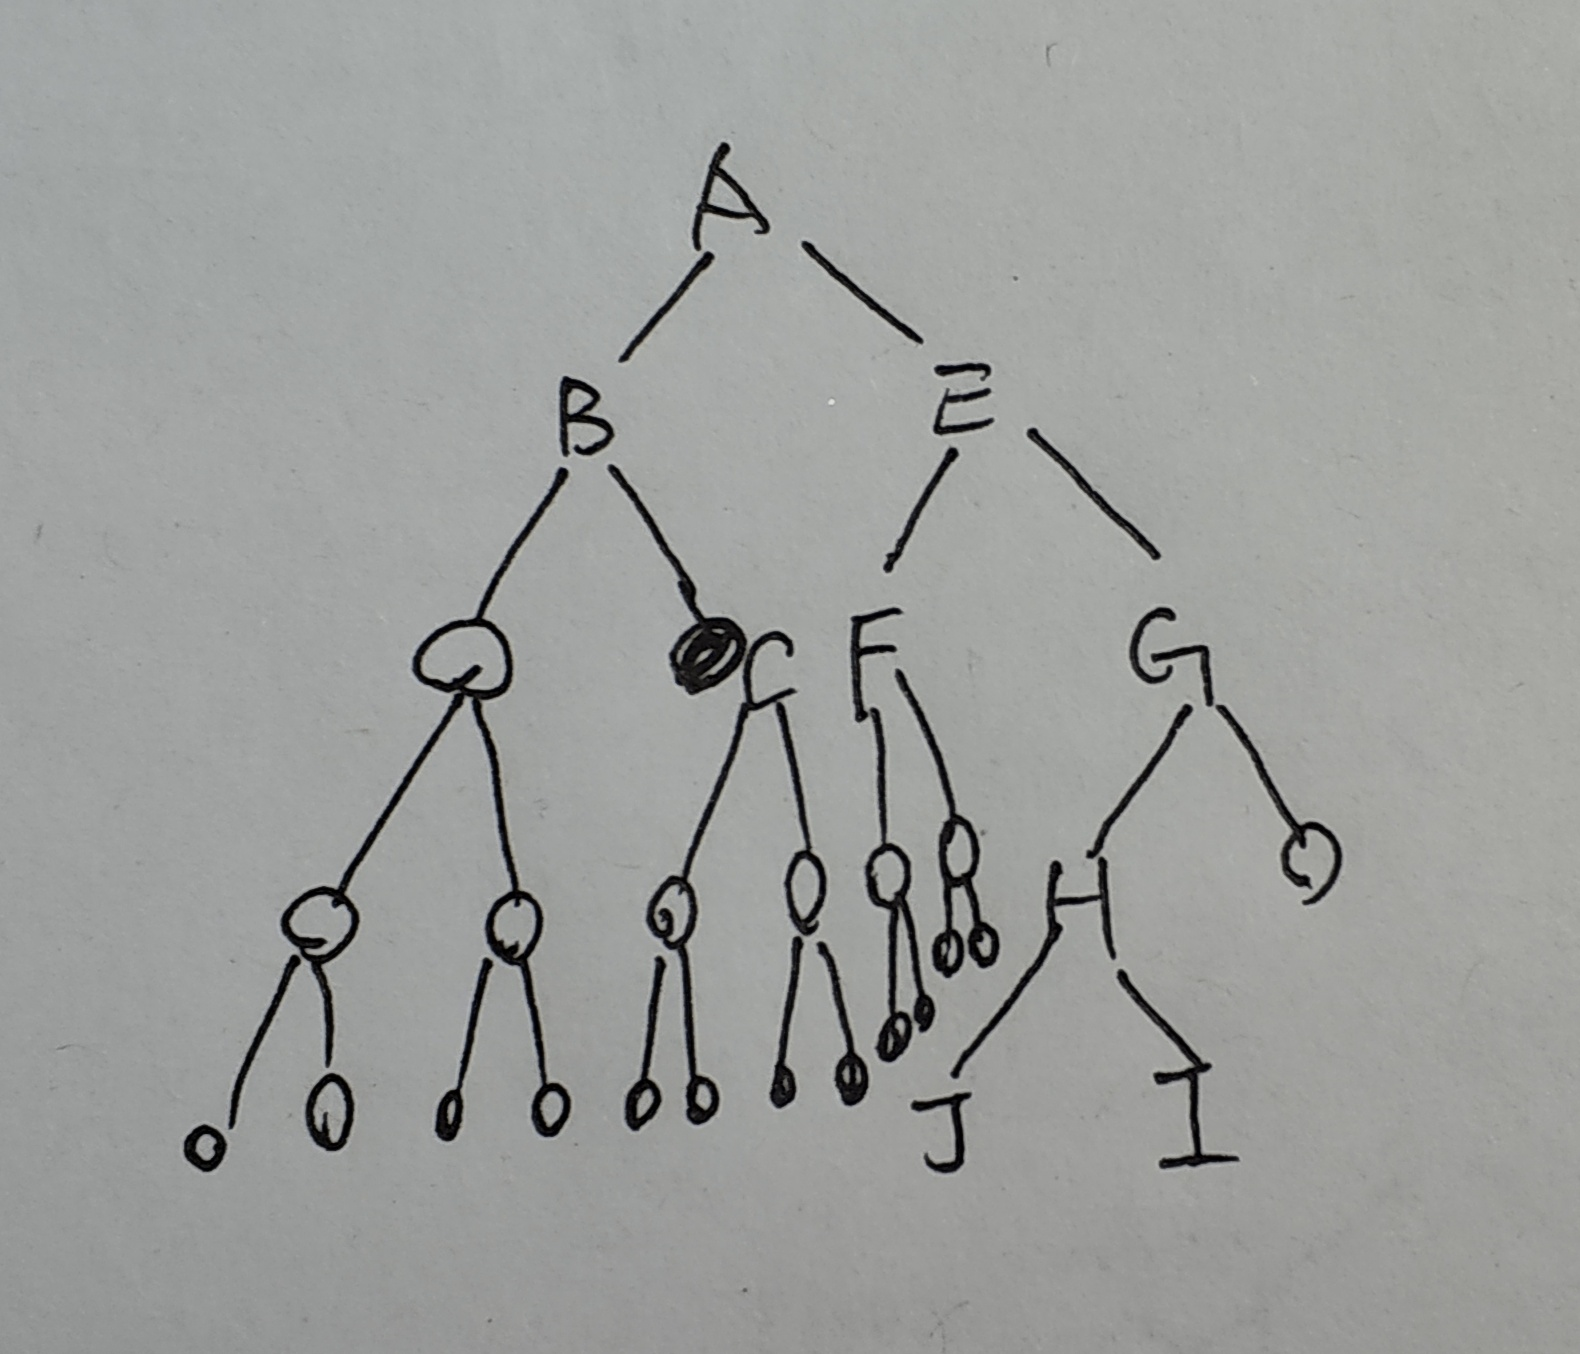
\includegraphics[scale=0.3]{example/chapter2/IMG_20181127_170103.png}
\end{figure}
~\\
顺序存储结构如下\newline
\begin{center}
\begin{tabular}{|c|c|c|c|c|c|c|c|c|c|}% 通过添加 | 来表示是否需要绘制竖线
	\hline  % 在表格最上方绘制横线
	0 & 1 & 2 & 3 & 4 & 5 & 6 & 7 & 8 & 9 \\
	\hline  % 在表格最上方绘制横线
	A & B & E &   & C & F & G &   &   &   \\
	\hline  % 在表格最上方绘制横线
	10 & 11 & 12 & 13 & 14 & 15 & 16 & 17 & 18 & 19 \\
	\hline  %在第一行和第二行之间绘制横线
	  &   &   & H &   &   &   &   &   &   \\
	\hline  % 在表格最上方绘制横线
	20 & 21 & 22 & 23 & 24 & 25 & 26 & 27 & 28 & 29 \\
	\hline  % 在表格最上方绘制横线
	  &   &   &   &   &   &   &  j & i  &   \\
	\hline  %在第一行和第二行之间绘制横线
\end{tabular}
\end{center}


\subsection{2011408}
若一棵完全二叉树有768个节点,则该二叉树中叶节点的个数是(   )\newline
解:\newline
1 + 2 + 4 + 8 + 16 + 32 + 64 + 128 +256 + 512 > 768\newline
1 + 2 + 4 + 8 + 16 + 32 + 64 + 128 +256 < 768\newline
$\frac{1*(1-2^9)}{1-2} = 511$,768 - 511 = 257 , 257 / 2 = 128.5 = 129, 256 - 129 = 127, 127 + 257 = 384.\newline
\\~ 
逻辑推理太复杂,简便的方法。应用完全二叉树的公式.  $ 当 i \le \lfloor n/2 \rfloor $ 则节点i为分支节点,否则为叶子节点。\newline
得到 768 / 2 = 384, 得到  768 - 384 = 384 则有384个叶子节点。\newline


\subsection{2014年408}
二叉树的带权路径长度(WPL)是二叉树中所有叶节点的带权路径长度之和。给定一棵二叉树T,采用二叉链表存储,节点结构为:'[left, weight, right]'其中叶节点的weight域保存该节点的非负权值、设root为指向T的根节点的指针,请设计求T的WPL的算法,要求:\newline
1) 给出算法的基本设计思想;\newline
2) 使用C或C++语言,给出二叉树节点的数据类型定义;\newline
3) 根据设计思想,采用C或C++语言描述算法,关键之处给出注释.\newline
解:\newline
1)\newline
设计思想是:层次遍历一层如果遇到是叶节点,那么计算这个节点的带权路径长度。\newline
\begin{lstlisting}[basicstyle=\small\ttfamily, caption={}, numbers=none]
#include <iostream>
#include <queue>
using namespace std;
typedef struct LNode {
	LNode *left;
	LNode *right;
	int weight;
}LNode;

int calcWPL(LNode *root) {
	queue<LNode*> q;
	q.push(root);
	q.push(NULL);
	int level = 1;
	int wpl = 0;
	while (!q.empty()) {
		LNode * out = q.front();
		//cout << out->weight << endl;
		//确定是第几层,加入特殊的符号
		if (out == NULL) {
			level++;
			q.pop();
			if (q.empty()) {
				break;
			}
			out = q.front();//新的层的新的元素
			q.pop();
			q.push(NULL);
		}
		else {
			q.pop();
		}
		wpl += out->weight * level;
		cout << "[DEBUG weight] " << out->weight << endl;
		if (out->left!=NULL) {
			cout << "[DEBUG left]" << out->left->weight << endl;
			q.push(out->left);
		}
		if (out->right != NULL) {
			q.push(out->right);
			cout << "[DEBUG right]" << out->right->weight << endl;
		}
	}
	return wpl;
}


int main() {
// 构建二叉树
	LNode * root = (LNode *)malloc(sizeof(LNode));
	LNode * left1 = (LNode *)malloc(sizeof(LNode));
	LNode * right1 = (LNode *)malloc(sizeof(LNode));
	LNode * left1right = (LNode *)malloc(sizeof(LNode));
	LNode * left1left = (LNode *)malloc(sizeof(LNode));
	root->weight = 1; root->left = left1; root->right = right1;
	left1->weight = 2; left1->left = left1left; left1->right = left1right;
	right1->weight = 3; right1->left = NULL; right1->right = NULL;
	left1right->weight = 5; left1right->left = NULL; left1right->right = NULL;
	left1left->weight = 4; left1left->left = NULL; left1left->right = NULL;
	//
	cout << "WPL is: " << calcWPL(root) << endl;
	system("pause");
}
\end{lstlisting}
参考链接层次遍历寻找特定的层:\url{https://blog.csdn.net/OrthocenterChocolate/article/details/37612183}\newline
当然,先序遍历的方式更好。\newline
\begin{lstlisting}[basicstyle=\small\ttfamily, caption={}, numbers=none]
int WPL(BiTree Root){
	return wpl_PreOrder(root, 0);
}
int wpl_PreOrder(BiTree root, int deep){
	static int wpl = 0;
	if(root->lchild==NULL&&root->rchild==NULL){
		wpl+=deep*root->weight;
	}
	if(root->lchild!=NULL){
		wpl_PreOrder(root->lchild, deep+1);
	}
	if(root->rchild!=NULL){
		wpl_PreOrder(root->rchild, deep+1);
	}
	return wpl;
}
\end{lstlisting}

\subsection{2016年408选择题}
若森铃F有15条边、25个节点,则F包含树的个数是(  ) \newline
解:\newline
25 - 15 = 10 ==> 有10棵树。

\subsection{2011年408 \&\&  杭电2019年选择题}
已知一棵有2011个节点的树,其叶节点个数为116,该树对应的二叉树中五右孩子的结点个数是(   )\newline
A. 115  B. 116  C. 1895  D. 1896\newline














 % 树和二叉树 新增一丢丢 
%%# -*- coding: utf-8-unix -*-
%%==================================================
\chapter{哈夫曼树}
\label{chap3}

\begin{itemize}[noitemsep,topsep=0pt,parsep=0pt,partopsep=0pt]
	\item 知识点:讲解相关知识点。
	\item 题型:直接上真题。
\end{itemize}

\section{知识点和方法论}

\subsection{知识点}
\begin{itemize}[noitemsep,topsep=0pt,parsep=0pt,partopsep=0pt]
	\item 带权路径长度计算$$ WPL = \sum \mbox{节点的值} * \mbox{到这个节点的边的条数} $$
\end{itemize}


\subsection{方法论}
\begin{itemize}[noitemsep,topsep=0pt,parsep=0pt,partopsep=0pt]
	\item 左小右大(虽然不一定要这么做)
	\item 左0右1
\end{itemize}


\section{真题实战}


\subsection{2015年}

\begin{lstlisting}[basicstyle=\small\ttfamily, caption={}, numbers=none]
给定集合{15 , 3 , 14, 2 , 6 , 9, 16,17}
1) 用矩形表示外部结点,用圆圈表示内部节点,构造相应的哈夫曼树;
2) 算带权路径长度;
3) 写出哈夫曼编码;
\end{lstlisting}
~\\
解:\newline
\begin{figure}[H]
	\centering  % 环境中的内容居中排版
	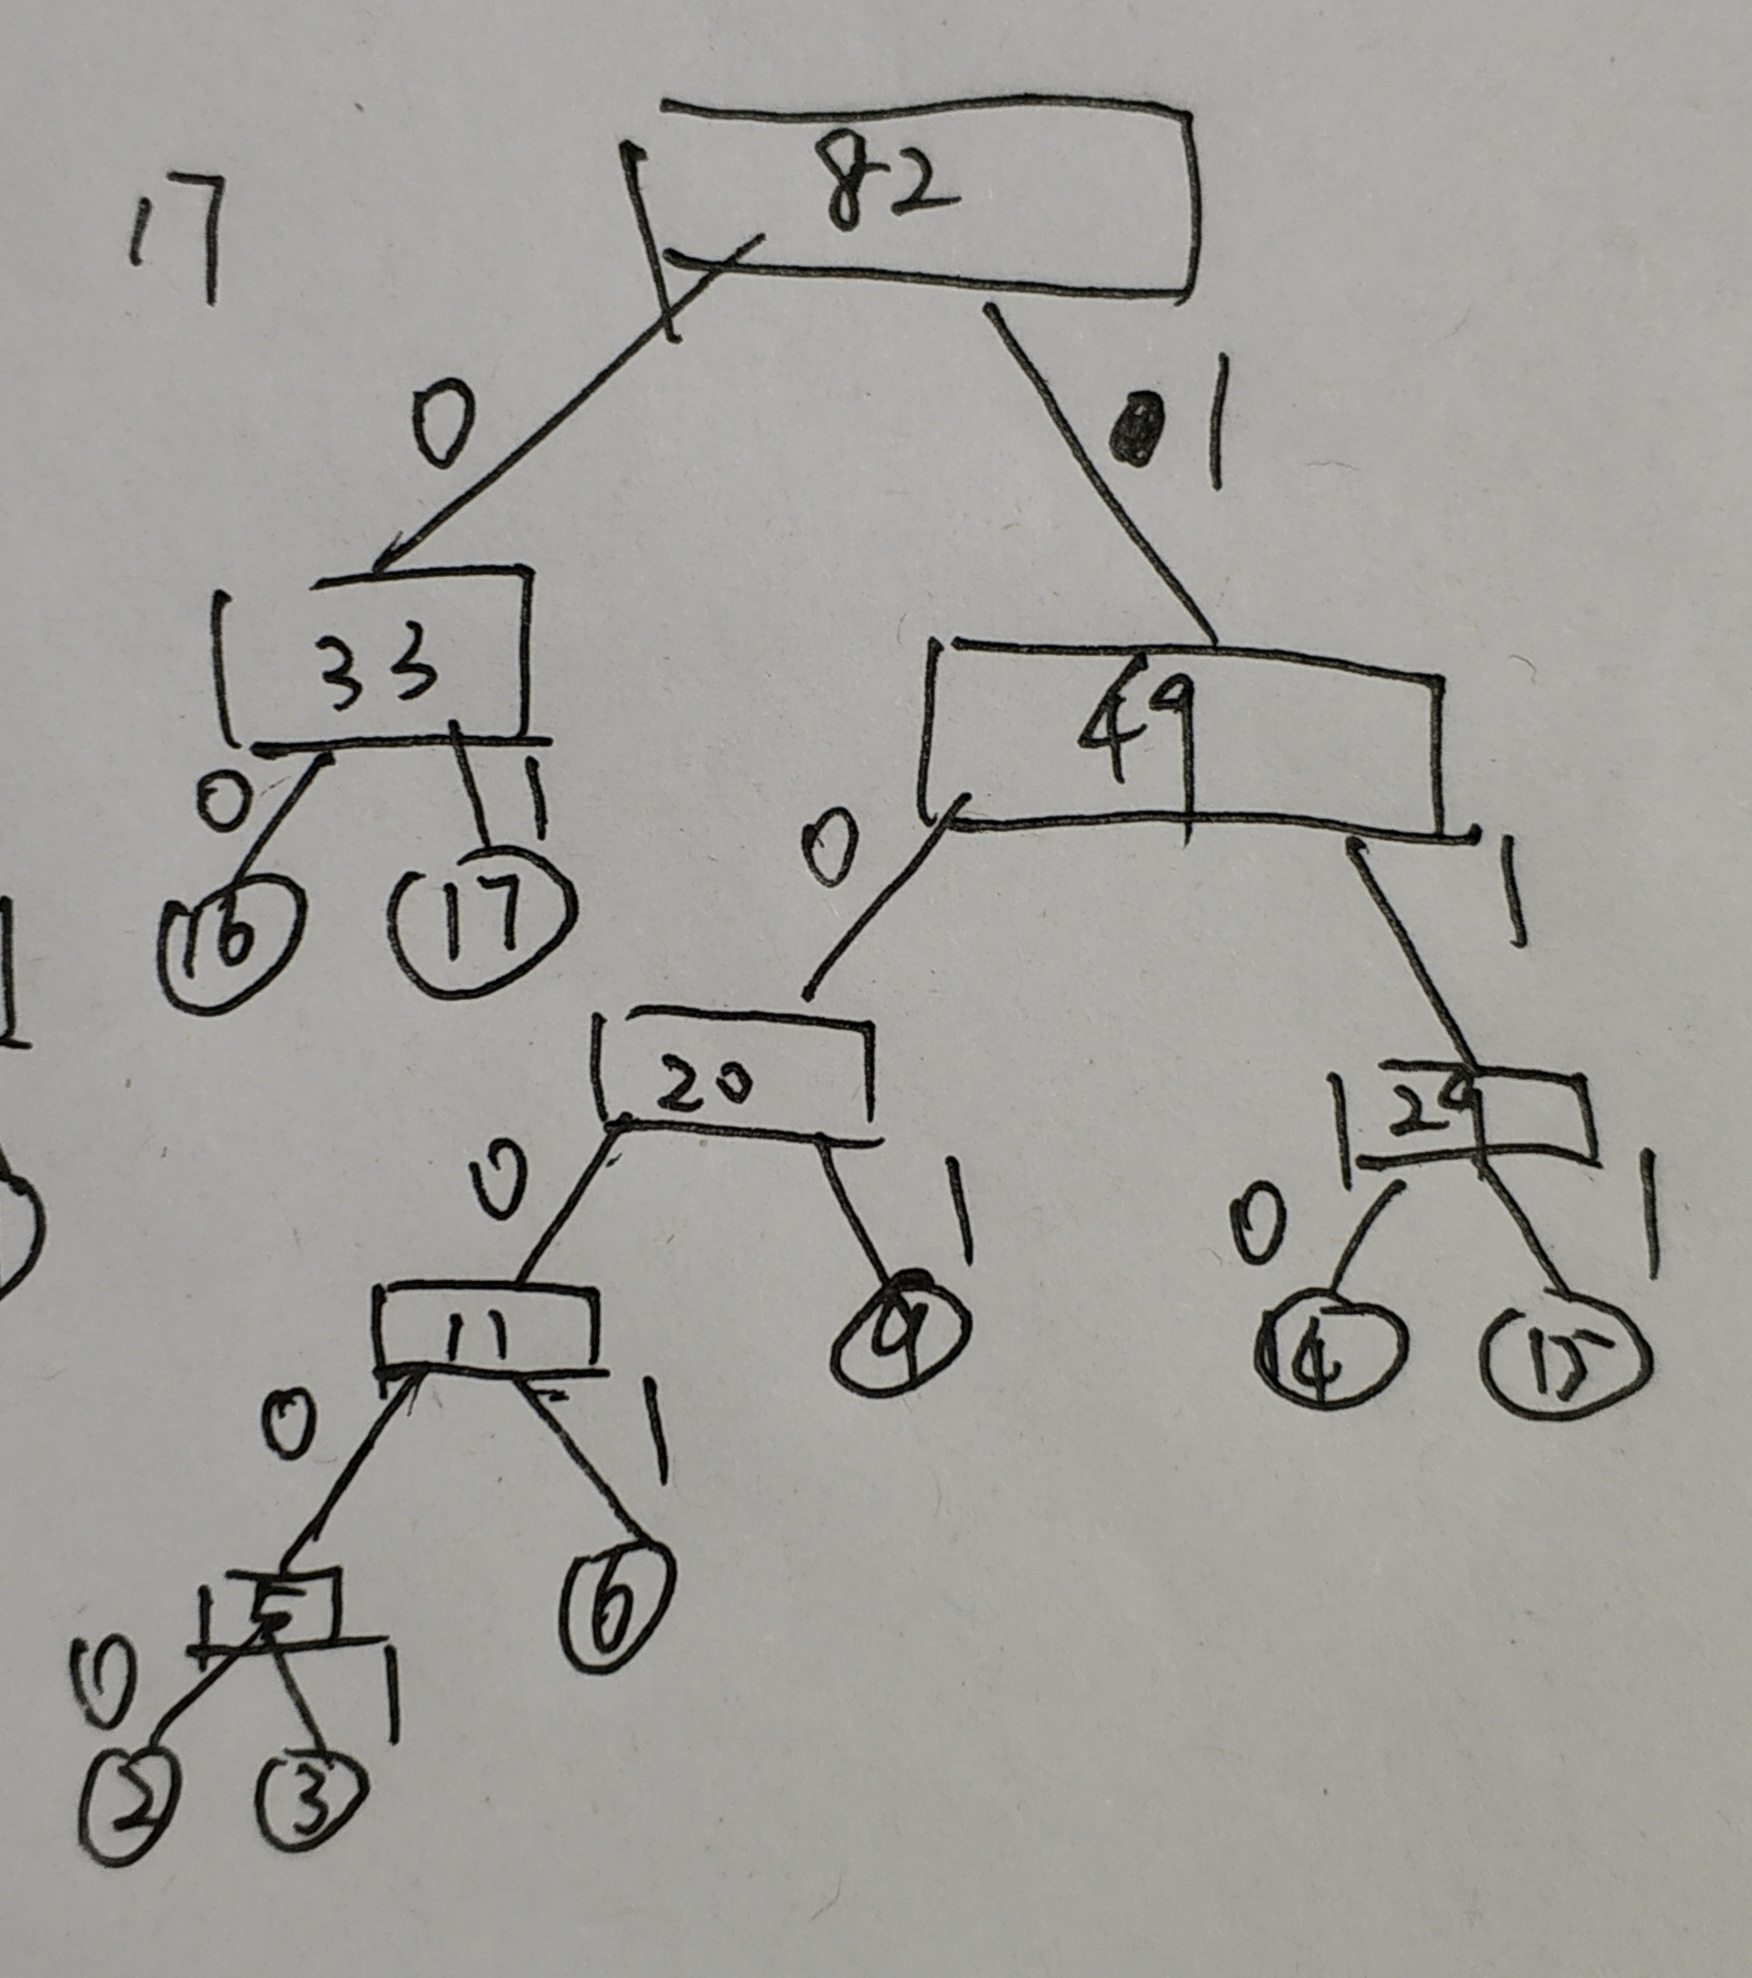
\includegraphics[scale=0.3]{example/chapter3/IMG_20181127_210022.png}
\end{figure}

2)\newline
$$ WPL =  16 * 2 + 17 * 2 + 14 *3 + 15 * 3 + 9 *3 + 6 * 4 + (2+3)* 5 = 229 $$
3)\newline
15:111\newline
14:110\newline
9:101\newline
6:1001\newline
2:10000\newline
3:10001\newline
16:00\newline
17:01\newline


\subsection{2017年}
\begin{figure}[H]
	\centering  % 环境中的内容居中排版
	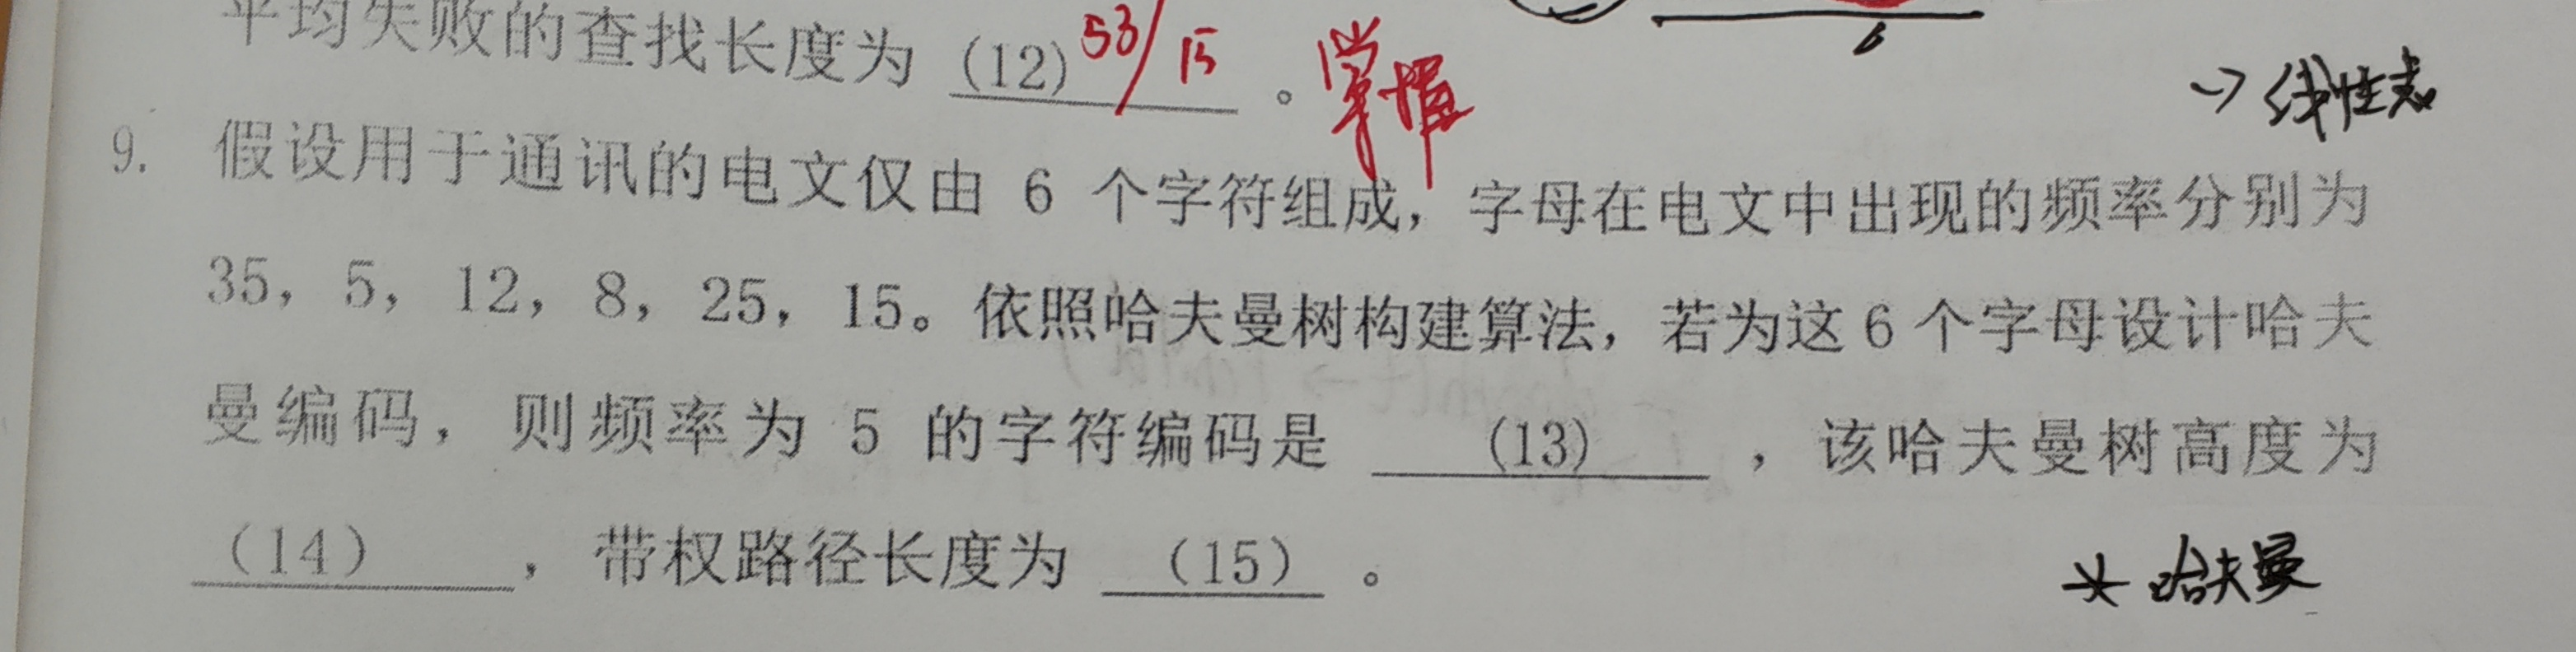
\includegraphics[scale=0.1]{example/chapter3/IMG_20181128_111603.png}
\end{figure}

解:\newline

\begin{figure}[H]
	\centering  % 环境中的内容居中排版
	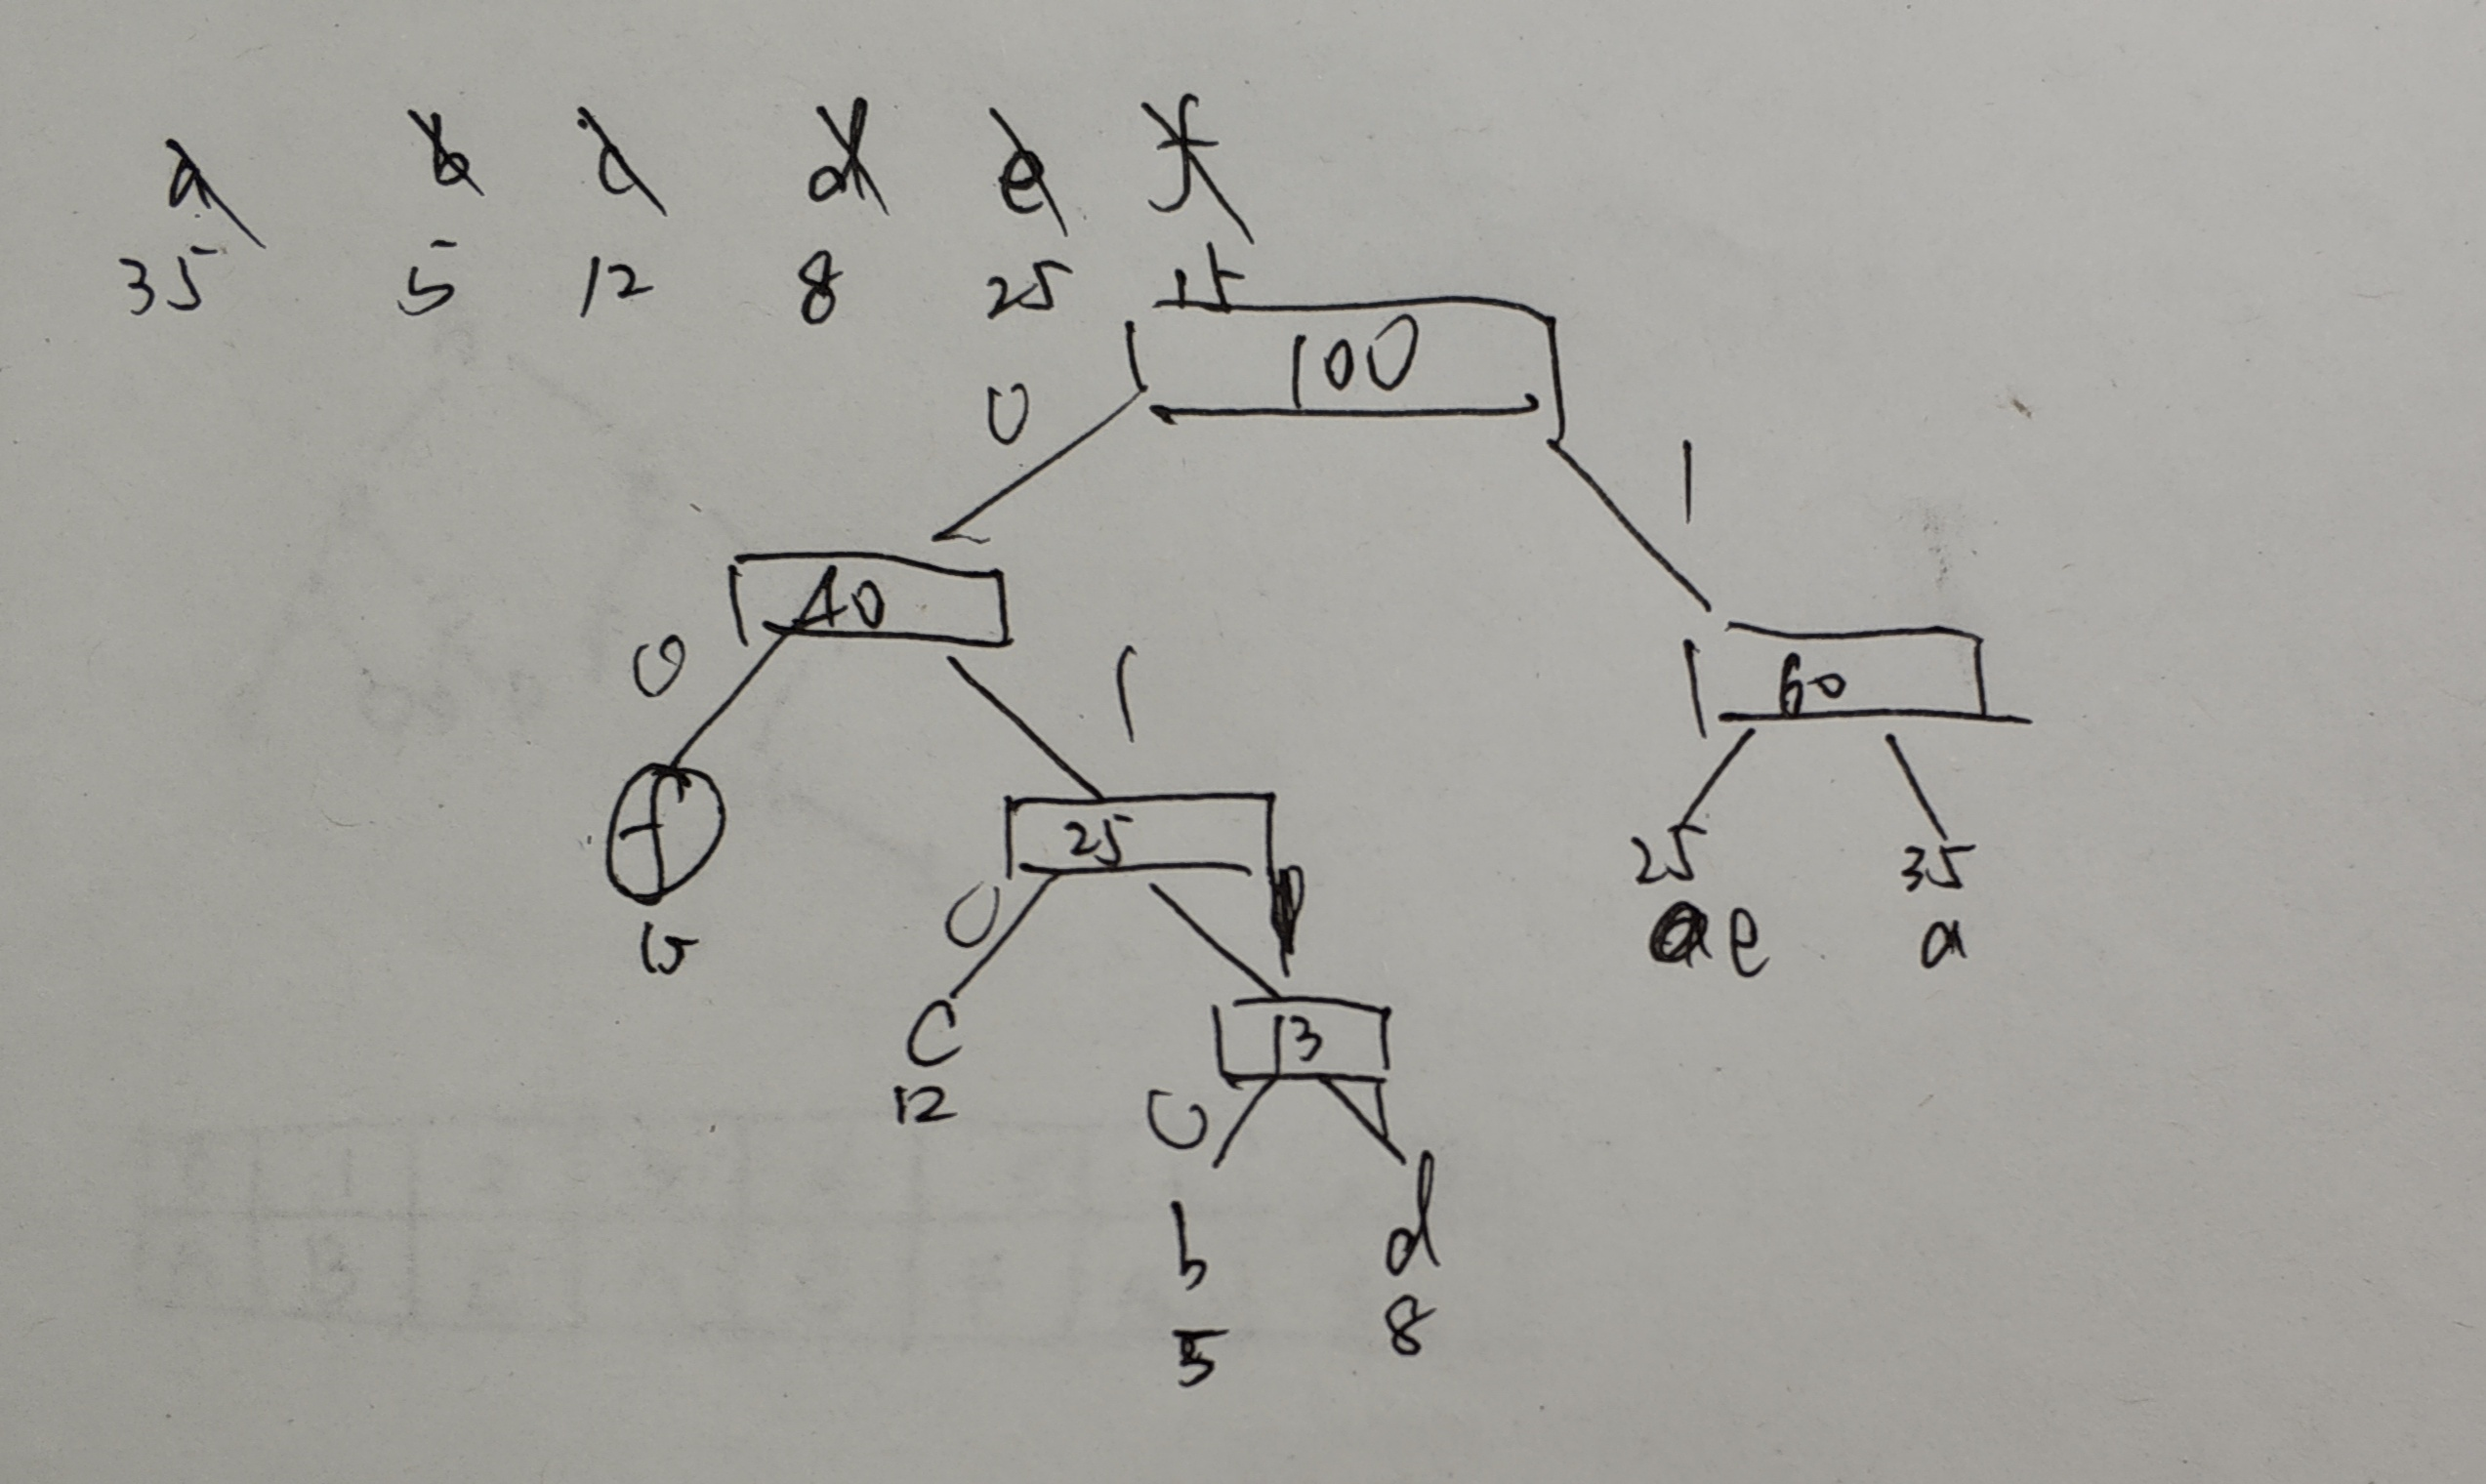
\includegraphics[scale=0.1]{example/chapter3/IMG_20181128_112049.png}
\end{figure}
~\\
5的编码 0110(不唯一,最好遵守左小右大,左0右1)\newline
高度   5\newline
$$WPL = (5*4 +8*4 + 12*3 + 15 *2 + 25 * 2 + 35 *2)=238 $$ % 哈夫曼树
%%# -*- coding: utf-8-unix -*-
%%==================================================
\chapter{广义表(了解)}
\label{chap4}

\begin{itemize}[noitemsep,topsep=0pt,parsep=0pt,partopsep=0pt]
	\item 知识点:讲解相关知识点。
	\item 题型:直接上真题。
\end{itemize}

\section{知识点和方法论}

\subsection{知识点}
\begin{itemize}[noitemsep,topsep=0pt,parsep=0pt,partopsep=0pt]
	\item 广义表只在严蔚敏书上P108有
	\item 例子
	\begin{itemize}[noitemsep,topsep=0pt,parsep=0pt,partopsep=0pt]
	\item $$ D = (A,B,C)$$
	\item GetHead(D) = A
	\item GetTail(D) = (B,C)
	\item 容易得到结论GetHead取出的是第一个{\color{red}元素},GetTail 取出的是除了第一个元素剩下的{\color{red}列表}
	\end{itemize}
\end{itemize}

\subsection{方法论}

\begin{itemize}[noitemsep,topsep=0pt,parsep=0pt,partopsep=0pt]
	\item 一层一层剥开
\end{itemize}

\section{真题实战}

\subsection{2017年第5题}
\begin{lstlisting}[basicstyle=\small\ttfamily, caption={}, numbers=none]
对广义表L=((a,b),((c,d),(e,f)))执行head(tail(head(tail(L))))操作的结果是___
\end{lstlisting}
解:\newline
L = ((a , b) , ((c,d),(e,f)))\newline
A = Tail(L) = (((c,d),(e,f)))\newline
B = Head(A) =((c,d),(e,f))\newline
C = tail(B) = ((e,f))\newline
D = head(C) = (e,f)\newline

\subsection{2016年第(12)题}
\begin{lstlisting}[basicstyle=\small\ttfamily, caption={}, numbers=none]
广义表((),(a),(b,(c,d),f))的深度为_____
\end{lstlisting}
解:\newline
\begin{figure}[H]
	\centering  % 环境中的内容居中排版
	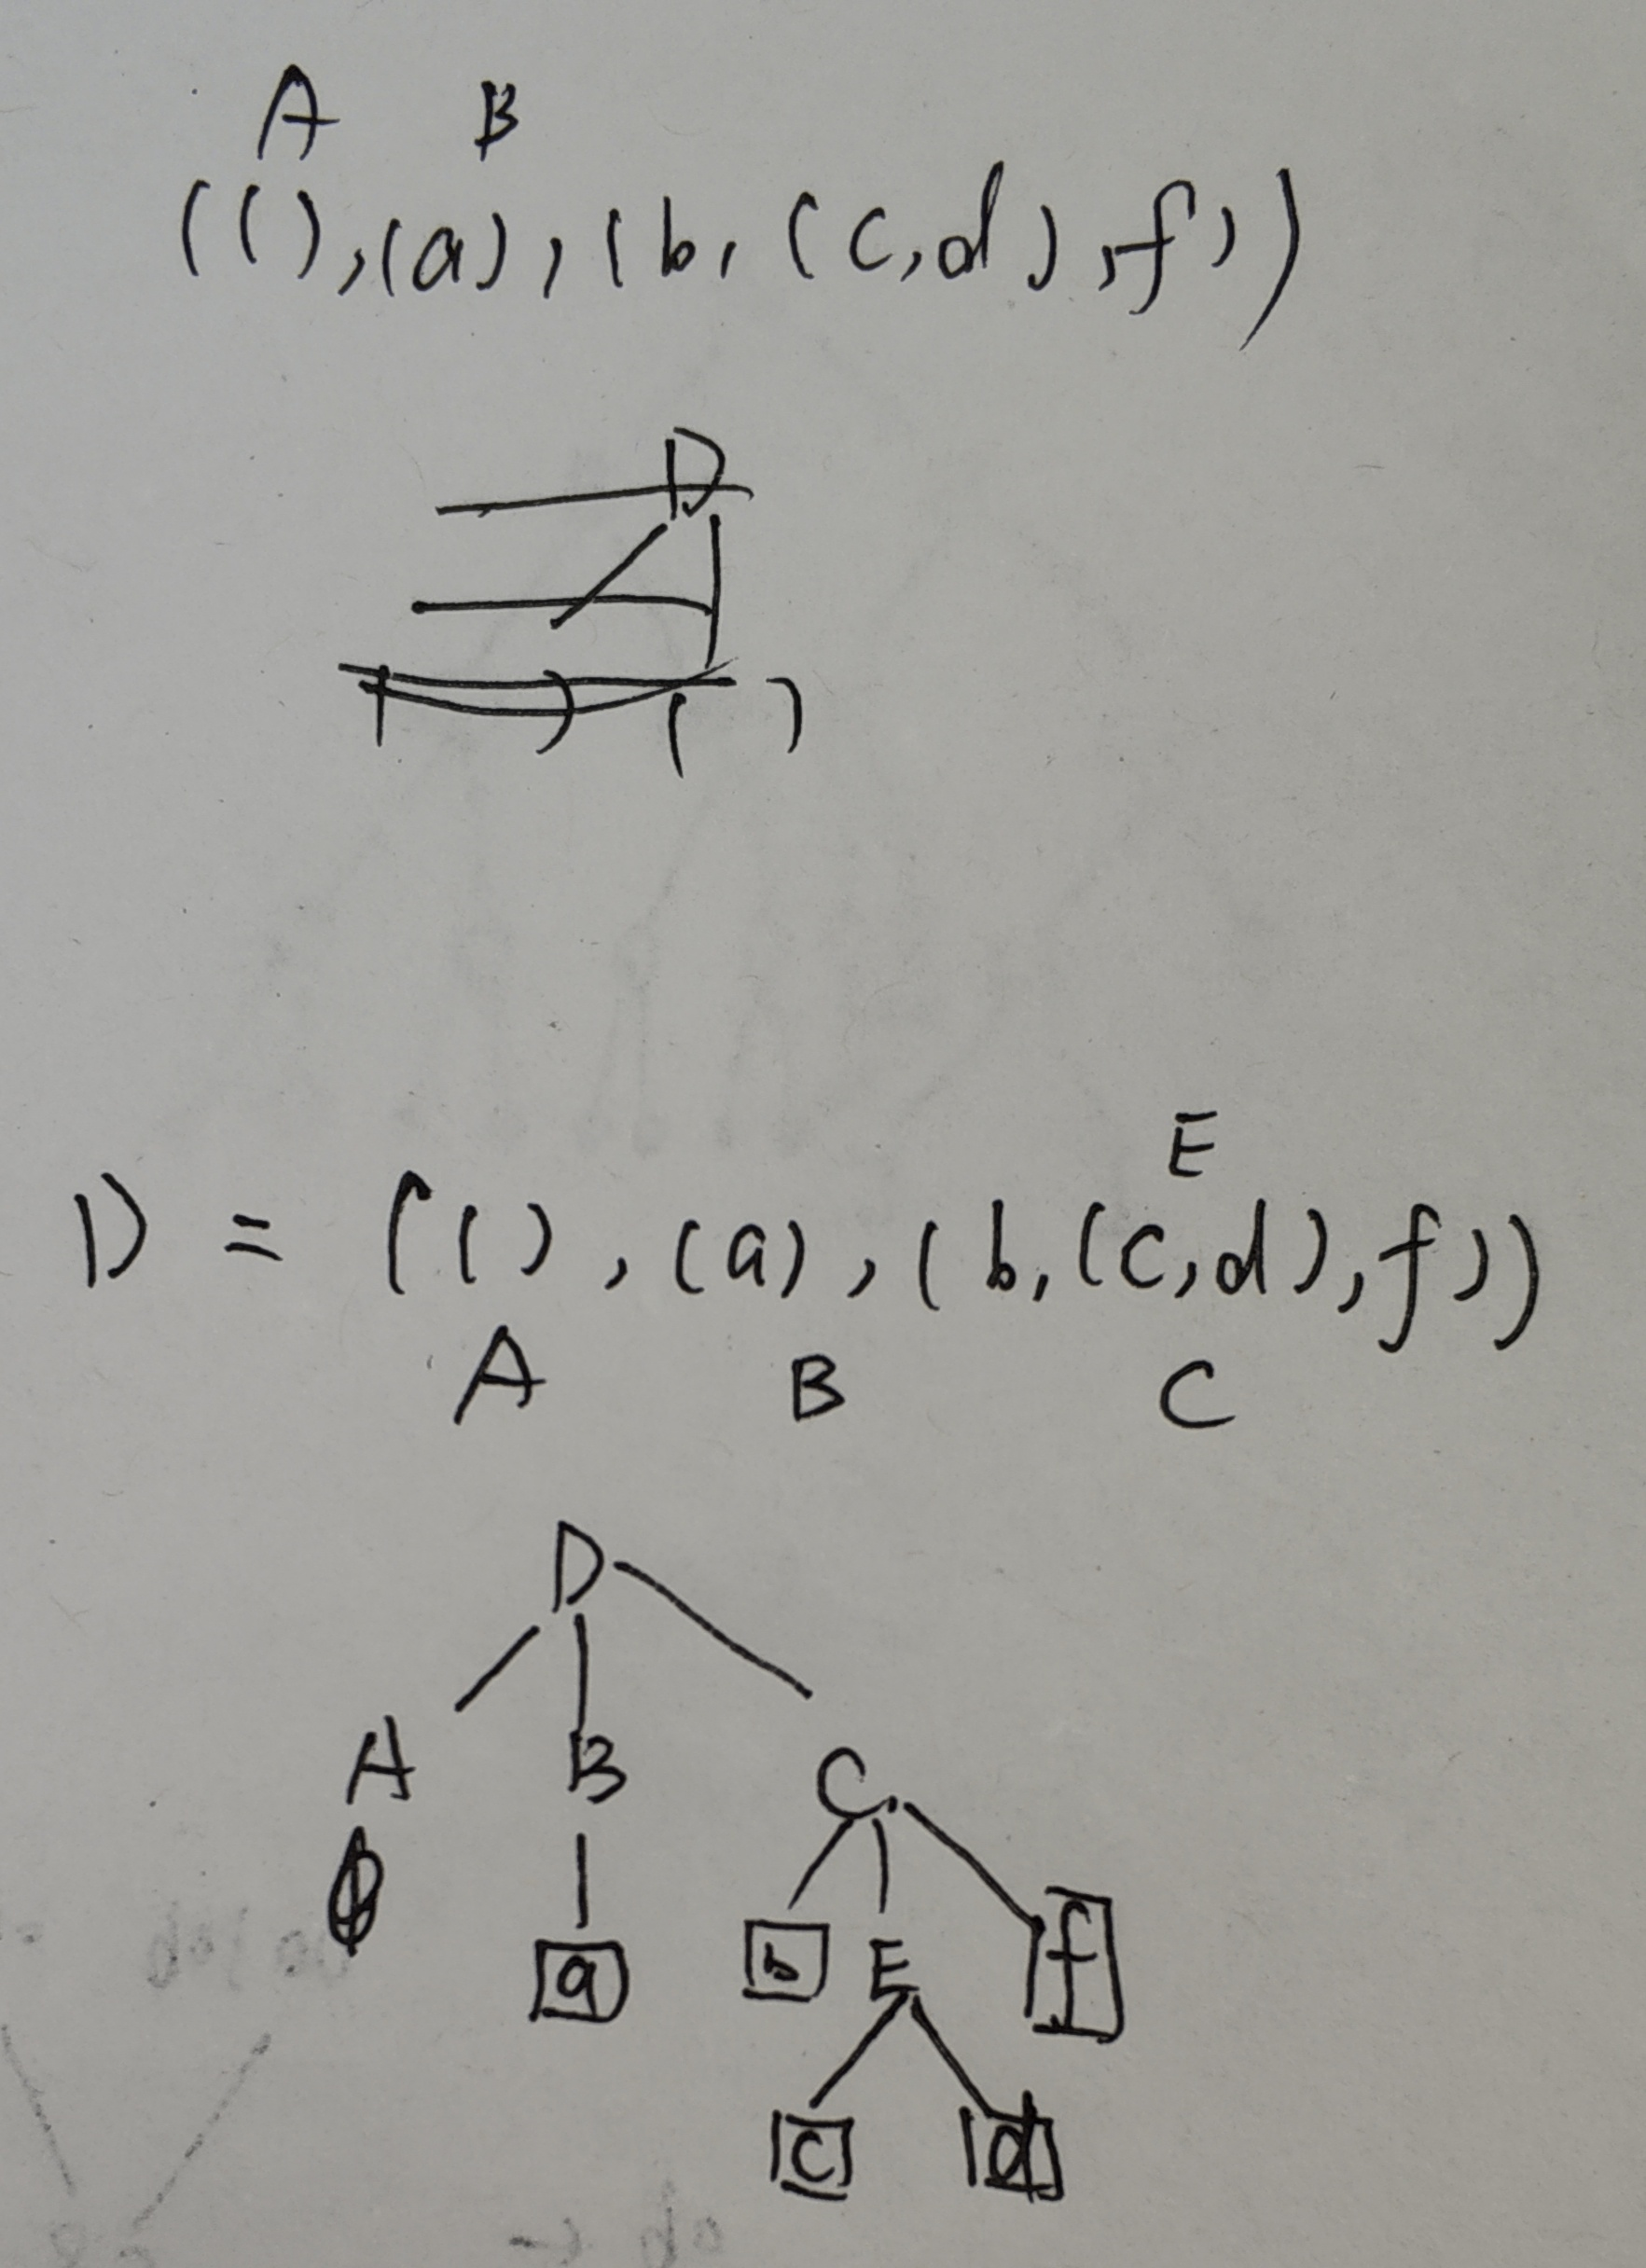
\includegraphics[scale=0.3]{example/chapter4/IMG_20181128_132004.png}
\end{figure}

求解深度参考链接\url{https://www.cnblogs.com/ciyeer/p/9040533.html}\newline
知道树的高度是4 但是最后一层是元素所以树的高度减去1就是广义表的深度。\newline

\subsection{2015年(5)}

\begin{lstlisting}[basicstyle=\small\ttfamily, caption={}, numbers=none]
已知广义表: A = (a,b), B = (A,A), C=(a,(b,A),B) 求下列运算的结果:tail(head(tail(C))) = (________)
\end{lstlisting}
解:\newline
C =(a,(b,A) ,B) \newline
  =(a,(b,(a,b)),((a,b),(a,b)) )\newline
Tail C =((b,(a,b)),((a,b),(a,b))) \newline
Head C' = (b,(a,b))\newline
Tail C'' = ((a,b))\newline
可知下划线上是  ((a,b)) - 即 (a,b)\newline % 广义表
%%# -*- coding: utf-8-unix -*-
%%==================================================
\chapter{Prim and Kruskal 算法}
\label{chap5}
\begin{itemize}[noitemsep,topsep=0pt,parsep=0pt,partopsep=0pt]
	\item 知识点:讲解相关知识点。
	\item 题型:直接上真题。
\end{itemize}
\section{知识点和方法论}


\subsection{知识点}

\begin{itemize}[noitemsep,topsep=0pt,parsep=0pt,partopsep=0pt]
	\item 无向图的邻接多重表的表示
	~\\
	\begin{center}
	\begin{tabular}{|c|c|c|c|c|c|}% 通过添加 | 来表示是否需要绘制竖线
		\hline  % 在表格最上方绘制横线
			Mark & Ivex & Ilink	& Jvex & Jlink & Info \\
		\hline  %在第一行和第二行之间绘制横线
	\end{tabular}
	\end{center}
	~\\
	\begin{center}
	\begin{tabular}{|c|c|}% 通过添加 | 来表示是否需要绘制竖线
		\hline  % 在表格最上方绘制横线
		 Data & firstedg \\
		\hline  %在第一行和第二行之间绘制横线
	\end{tabular}
	\end{center}

	\item 有向图的十字链表表示
	~\\
	\begin{center}
	\begin{tabular}{|c|c|c|}% 通过添加 | 来表示是否需要绘制竖线
		\hline  % 在表格最上方绘制横线
			Data & Firstin & Firstout\\
		\hline  %在第一行和第二行之间绘制横线
	\end{tabular}
	\end{center}
	~\\
	\begin{center}
	\begin{tabular}{|c|c|c|c|c|}% 通过添加 | 来表示是否需要绘制竖线
		\hline  % 在表格最上方绘制横线
		 Tailvex & Headvex & Hlink & Tlink & info \\
		\hline  %在第一行和第二行之间绘制横线
	\end{tabular}
	\end{center}
	\item 邻接矩阵表示法
	\item 邻接表表示法
\end{itemize}
\subsection{方法论}

\begin{itemize}[noitemsep,topsep=0pt,parsep=0pt,partopsep=0pt]
	\item 王道邻接多重表画法
	\begin{figure}[H]
	\centering  % 环境中的内容居中排版
	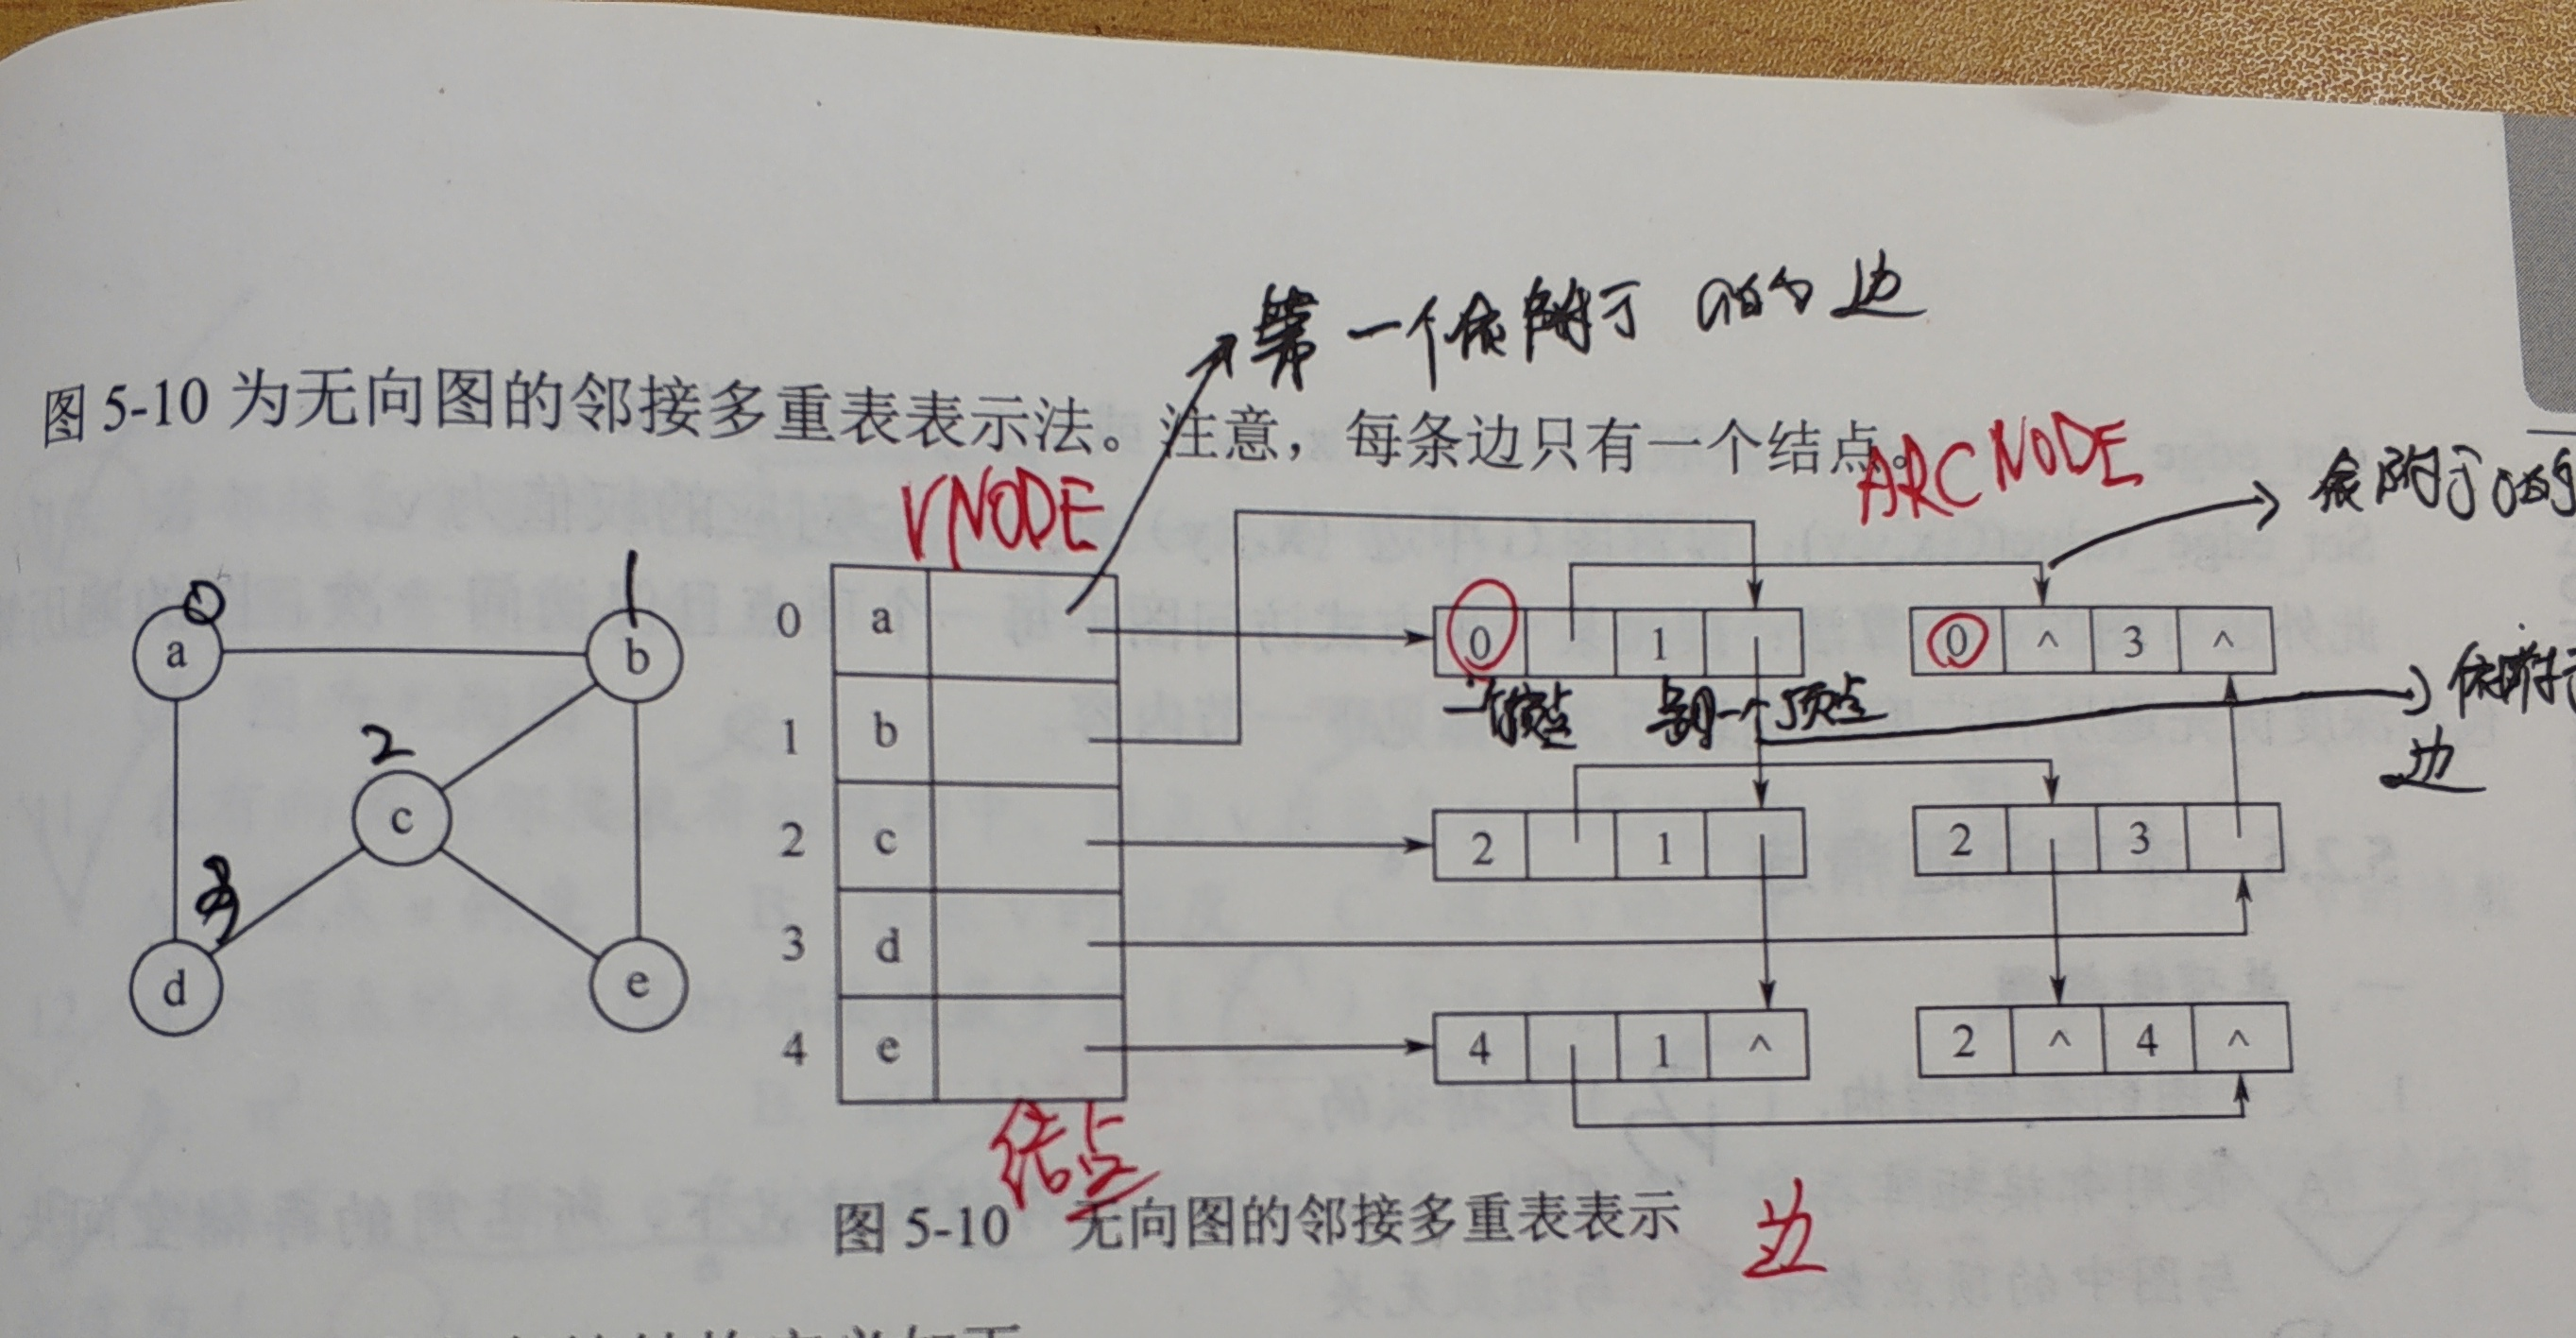
\includegraphics[scale=0.1]{example/chapter5/IMG_20181128_103024.png}
	\end{figure}
	\item 总共的空节点数量和顶点数量相同
\end{itemize}


\section{真题实战}


\subsection{2017年第3题}

\begin{figure}[H]
\centering  % 环境中的内容居中排版
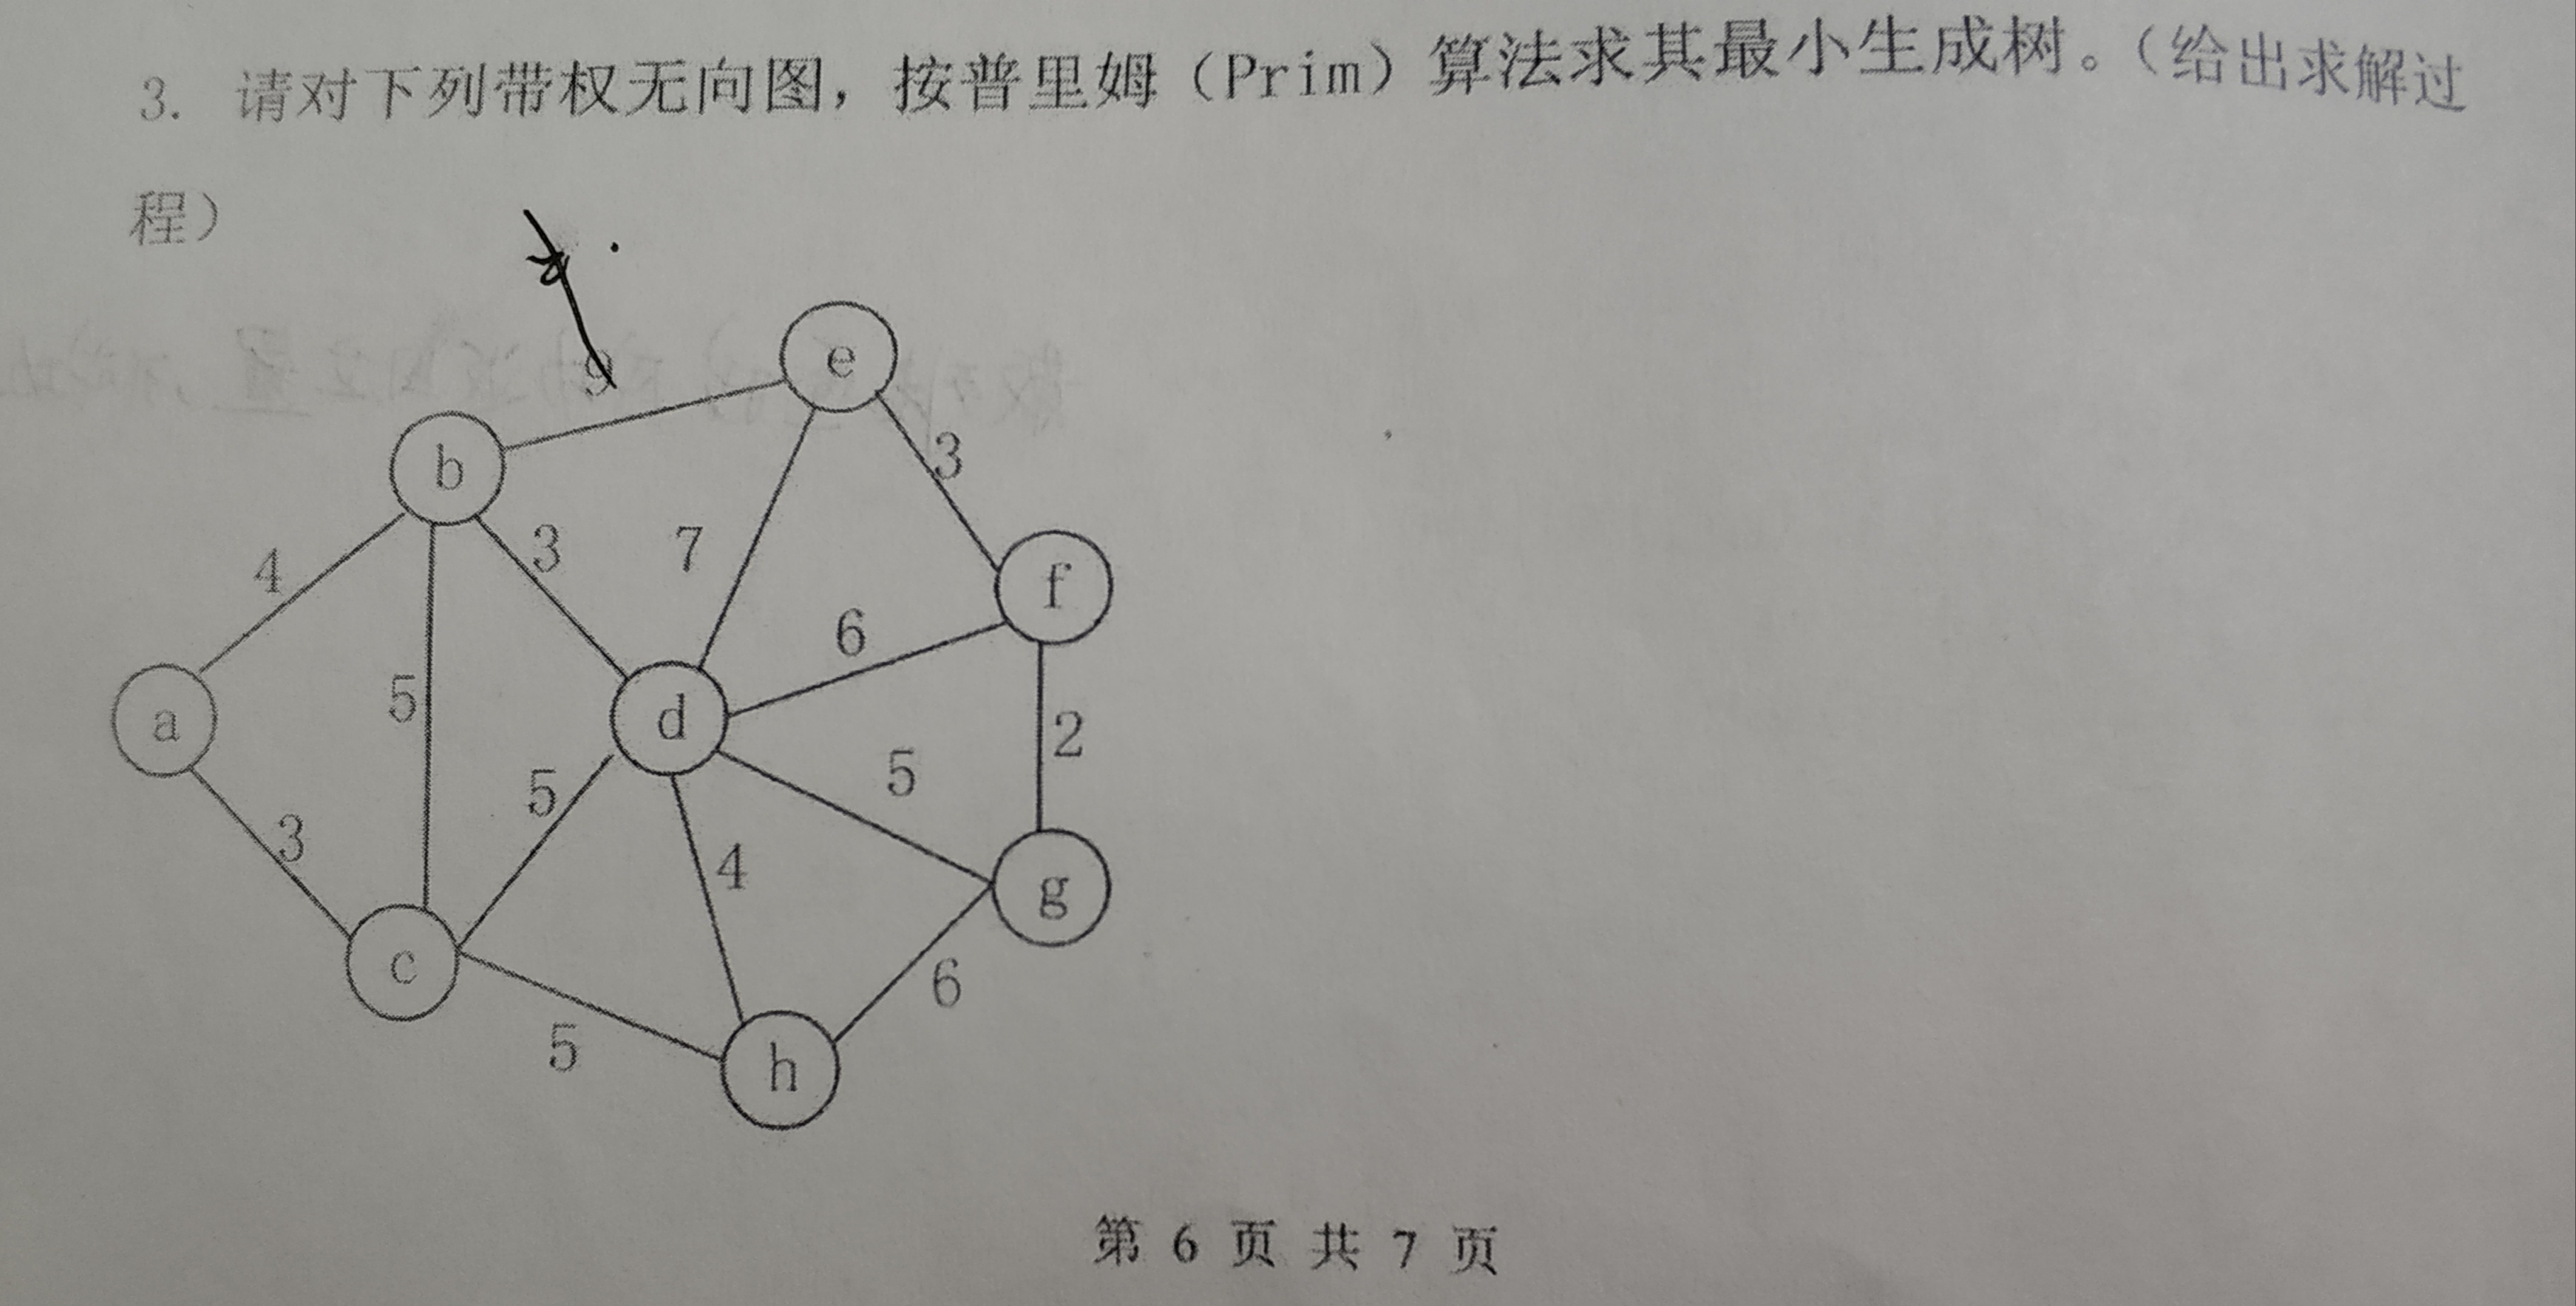
\includegraphics[scale=0.1]{example/chapter5/IMG_20181127_210442.png}
\end{figure}

解:\newline
严格按照严蔚敏的方式计算的话\newline
\begin{figure}[H]
\centering  % 环境中的内容居中排版
\includegraphics[scale=0.1]{example/chapter5/IMG_20181127_222510.png}
\end{figure}
注解  \newline
adjvex 那一行就是已经在生成树上的点到剩下的点最近的点\newline
下面紧挨着的就是距离,然后从中选出最短的距离,就是K值就是选中的点加入U集合\newline
一旦加入U集合下面就全部写0,U-K就是暂时不在生成树上的集合;\newline

\subsection{2016年(3)}
\begin{figure}[H]
\centering  % 环境中的内容居中排版
\includegraphics[scale=0.1]{example/chapter5/IMG_20181128_092826.png}
\end{figure}
解:\newline
~\\
1)\newline
\begin{lstlisting}[basicstyle=\small\ttfamily, caption={}, numbers=none]
Typedef struct ArcNode{
	Bool mark;
	Int ivex, jvex;
	Struct ArcNode *ilink,*jlink;
}ArcNode;
Typedef struct VNode{
	string data;                //顶点信息
	ArcNode *firstedge;
}VNode;
\end{lstlisting}
\begin{figure}[H]
\centering  % 环境中的内容居中排版
\includegraphics[scale=0.1]{example/chapter5/IMG_20181128_103404.png}
\end{figure}
2)\newline
\begin{figure}[H]
\centering  % 环境中的内容居中排版
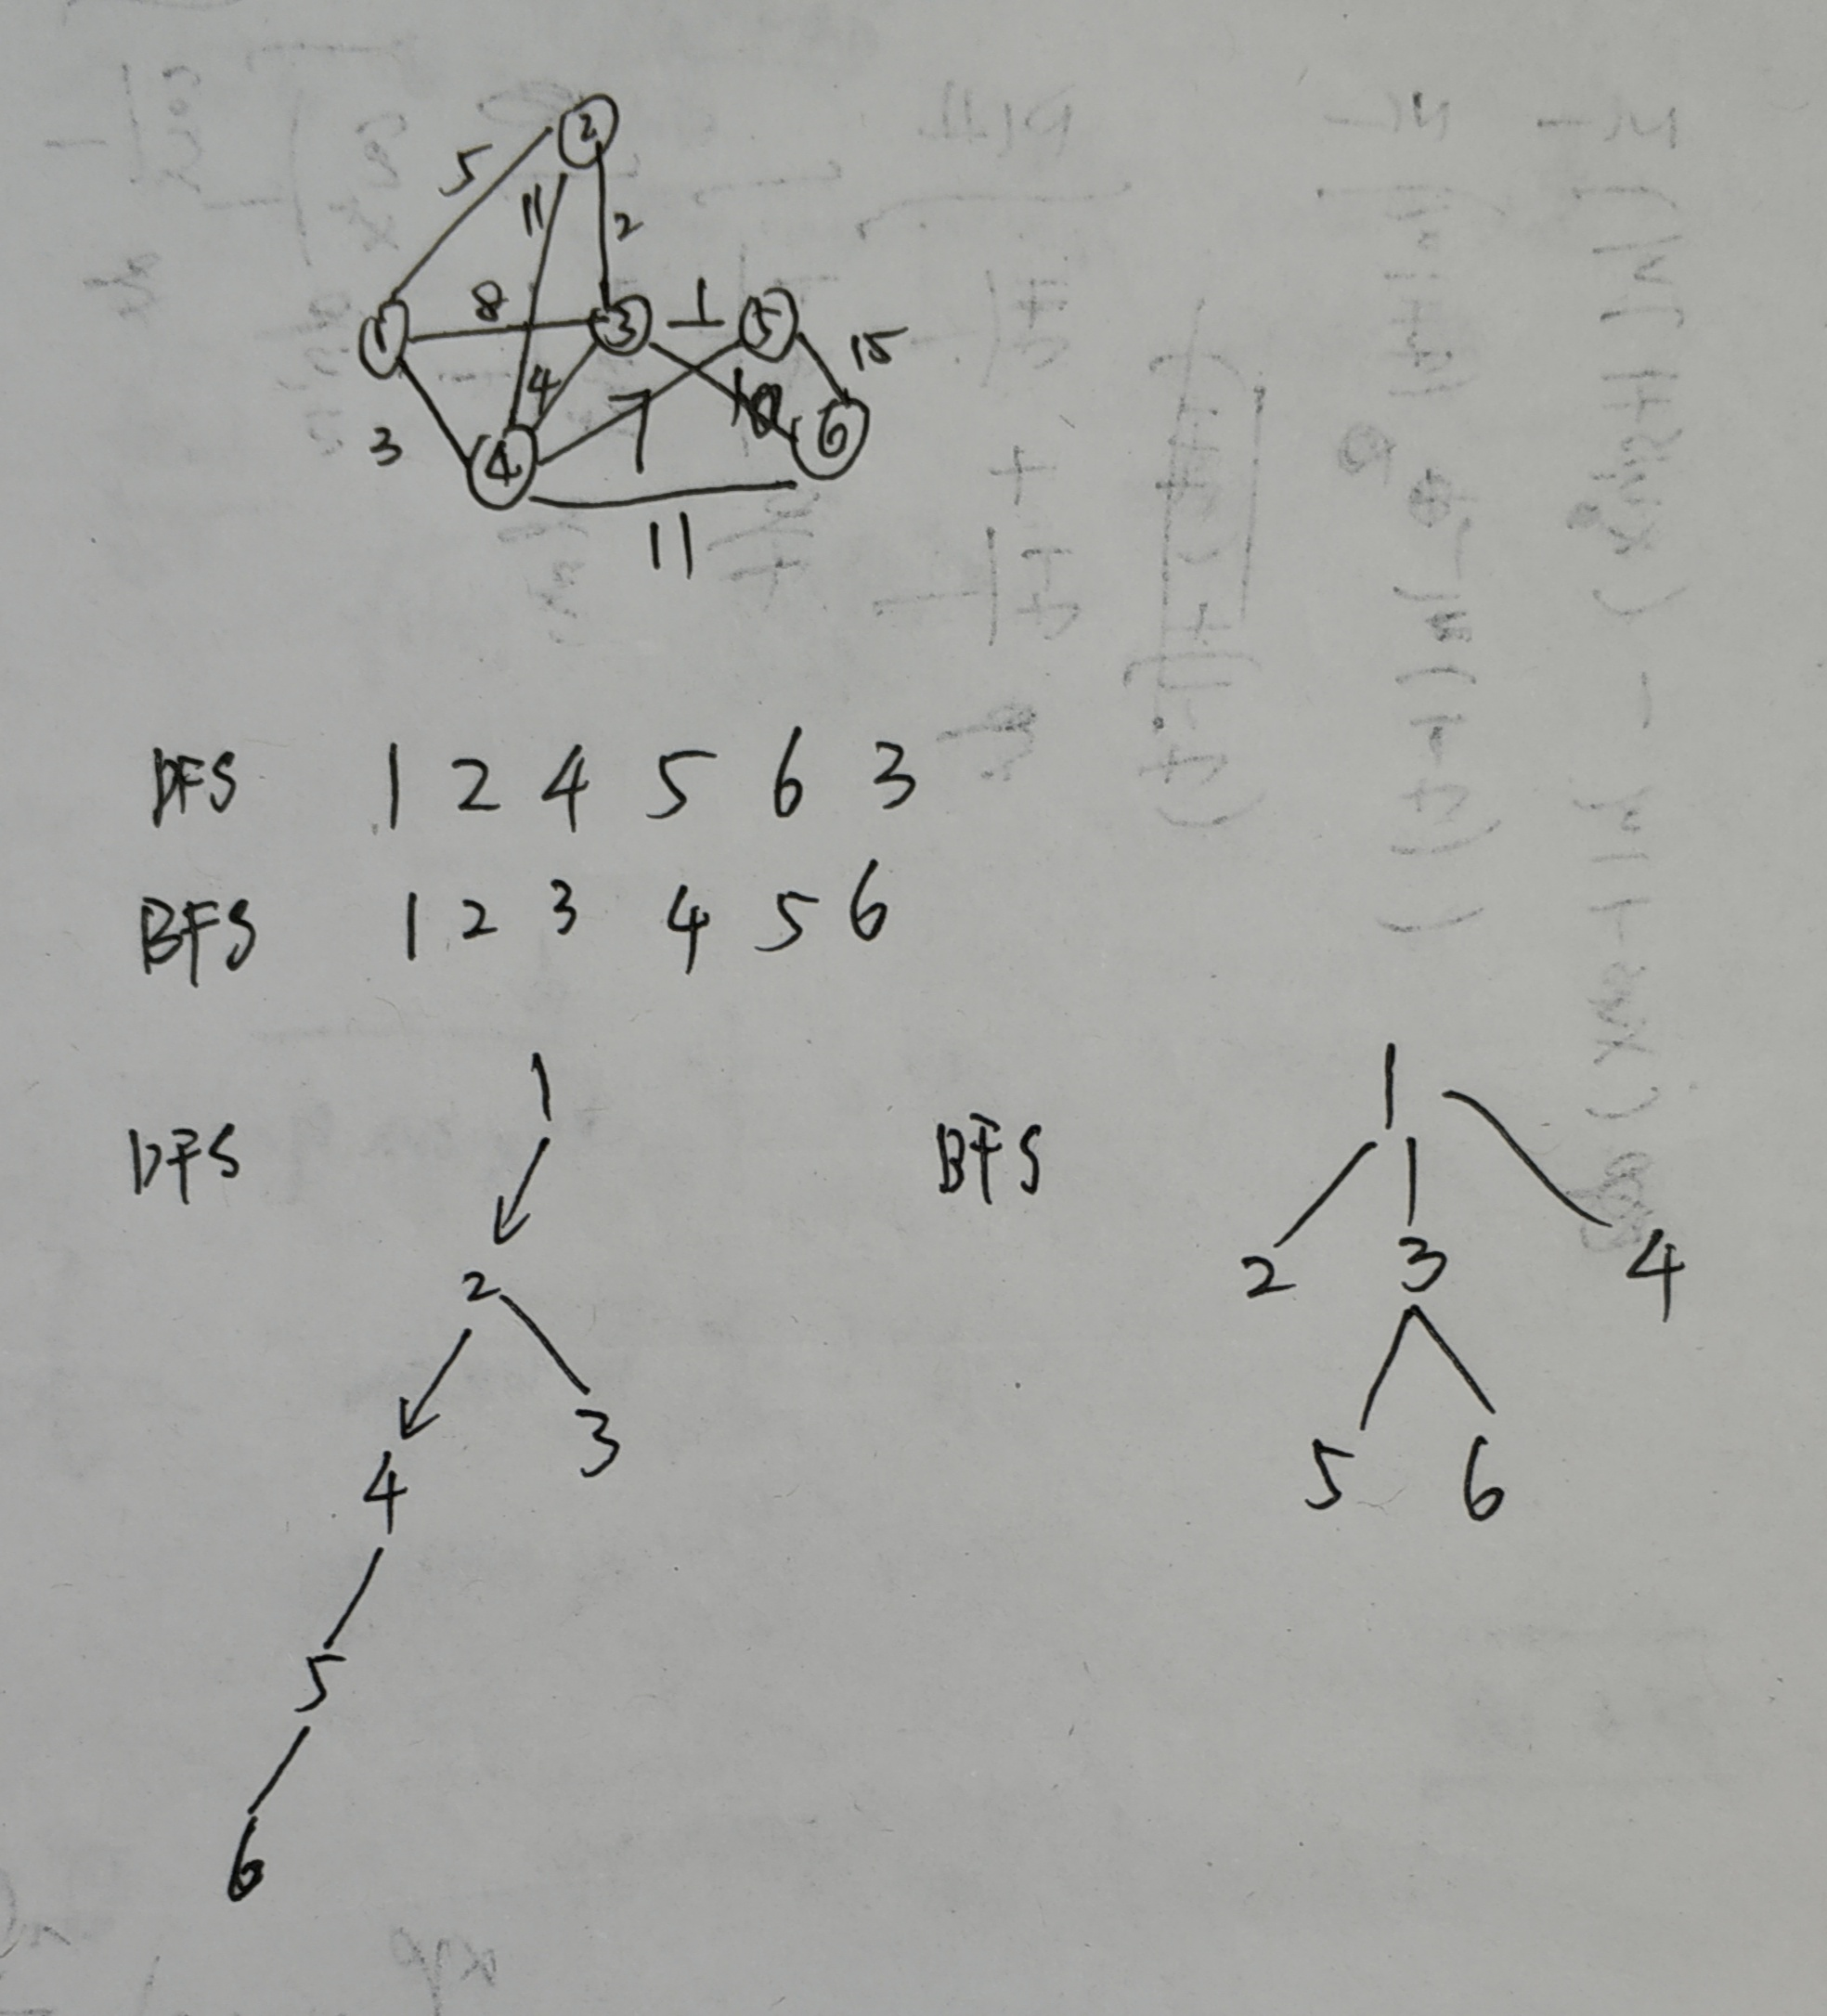
\includegraphics[scale=0.1]{example/chapter5/IMG_20181128_110619.png}
\end{figure}
3)\newline
最小生成树的边集{1,4},{1,2},{2,3},{3,5},{3,6} \newline
\begin{figure}[H]
\centering  % 环境中的内容居中排版
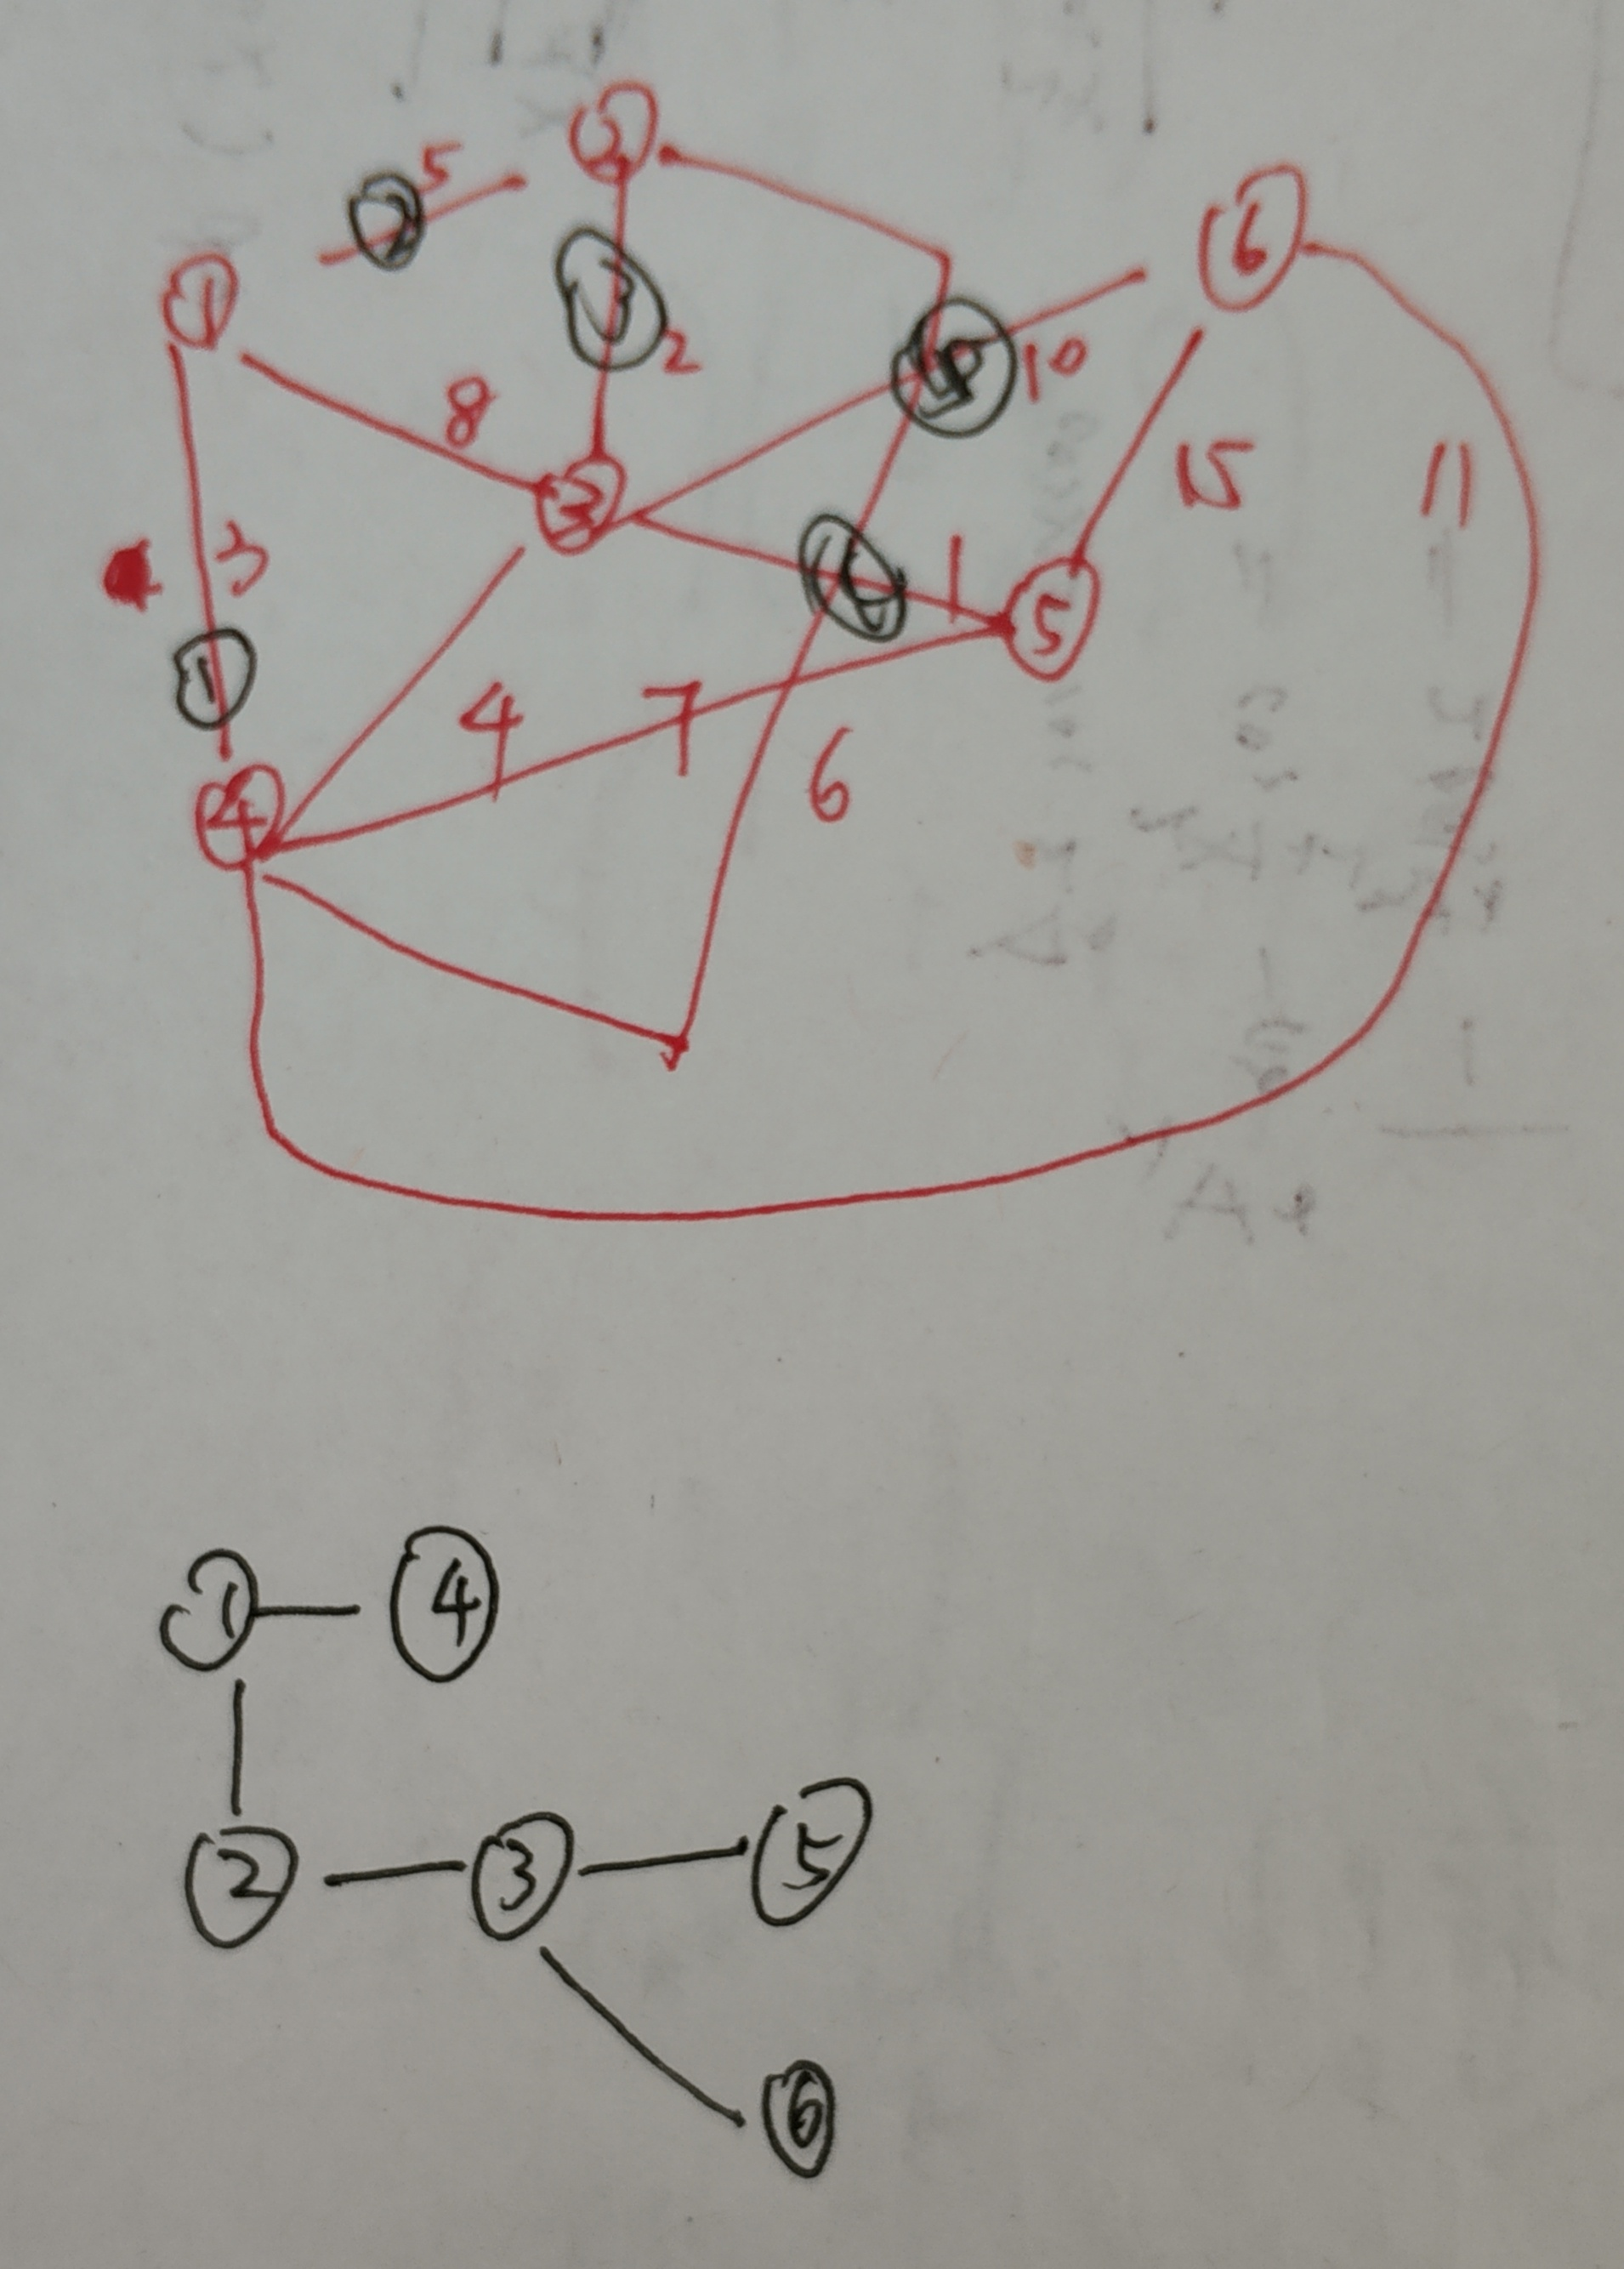
\includegraphics[scale=0.1]{example/chapter5/IMG_20181128_111203.png}
\end{figure}

\subsection{2014年第5题}


\begin{figure}[H]
\centering  % 环境中的内容居中排版
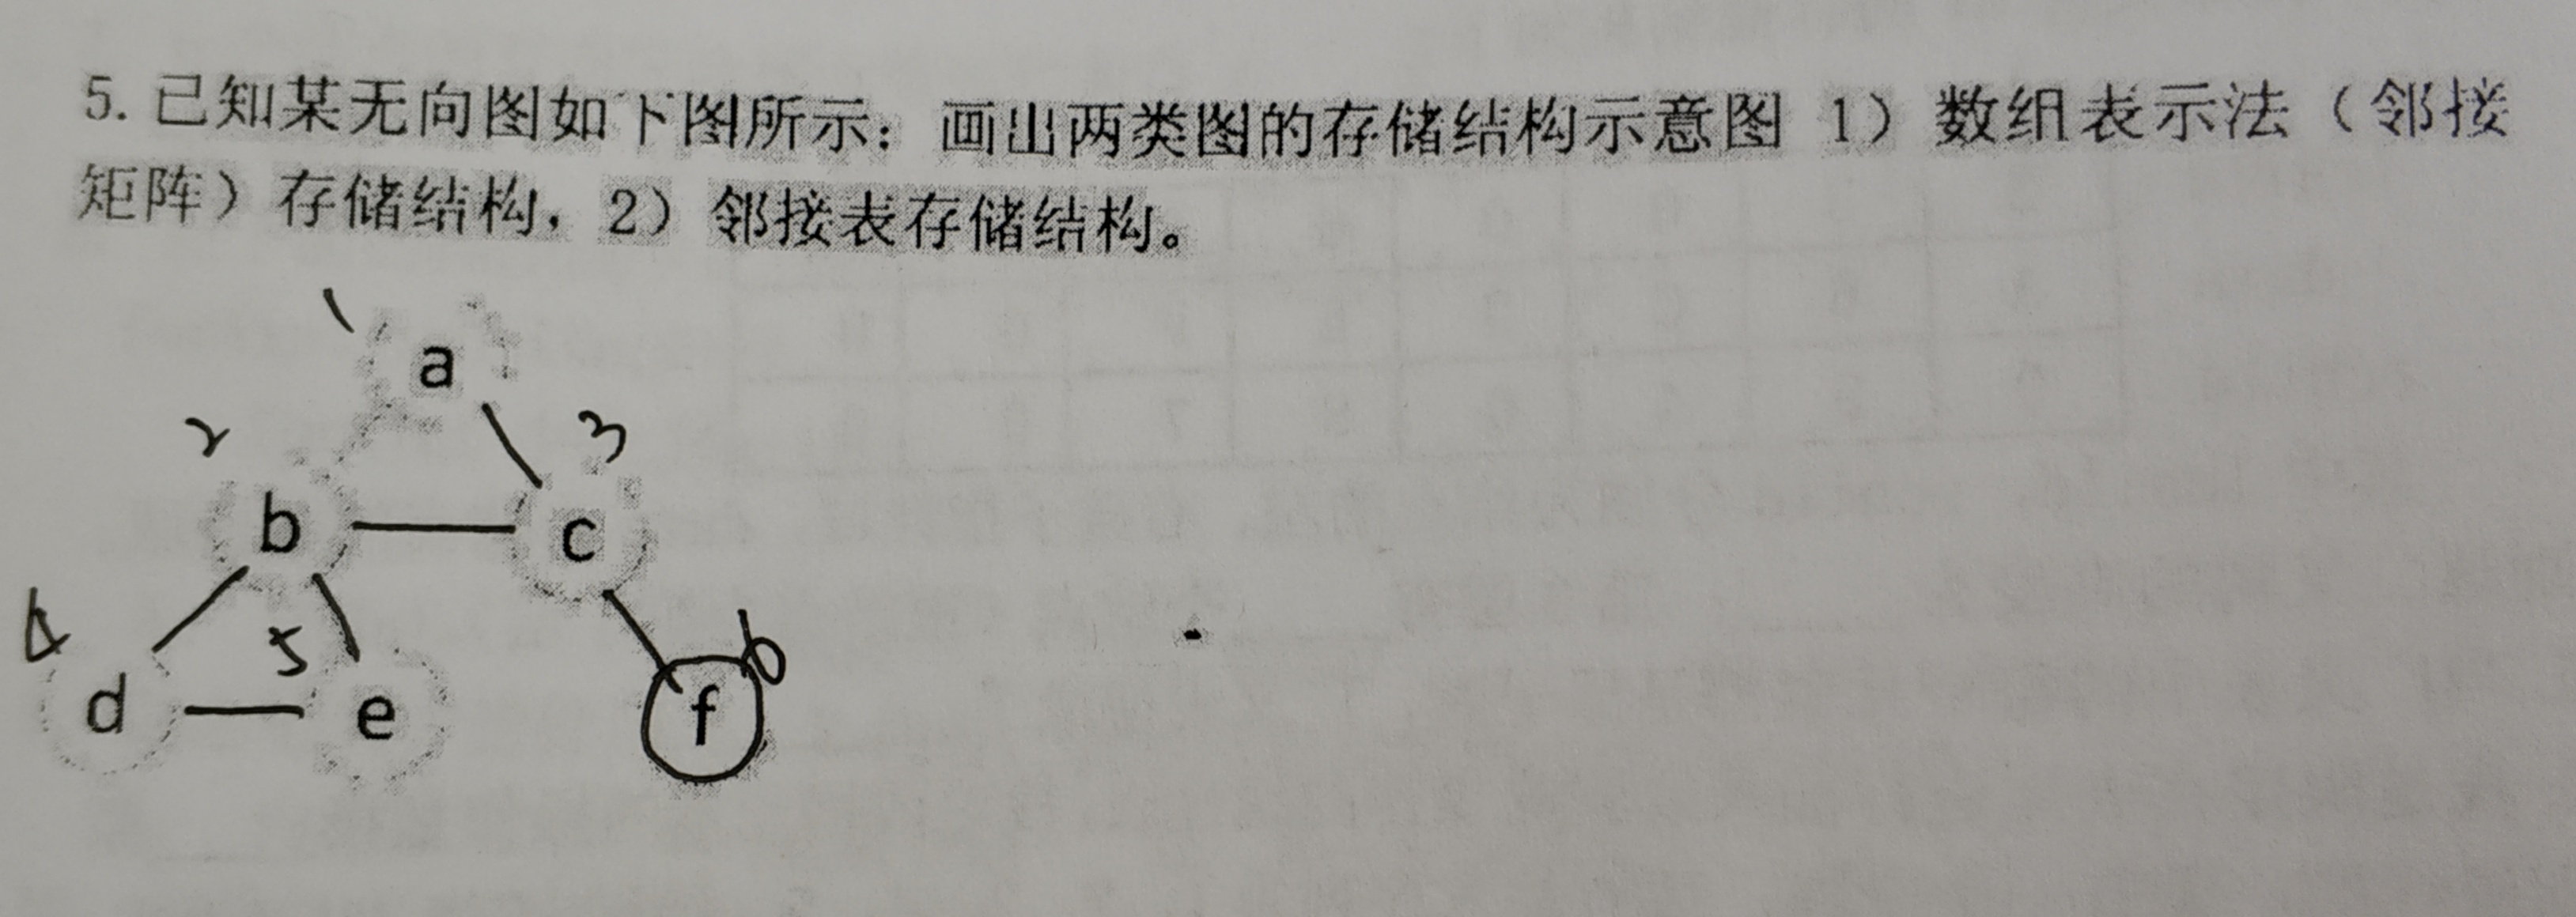
\includegraphics[scale=0.1]{example/chapter5/IMG_20181128_134713.png}
\end{figure}

解:\newline

\begin{figure}[H]
\centering  % 环境中的内容居中排版
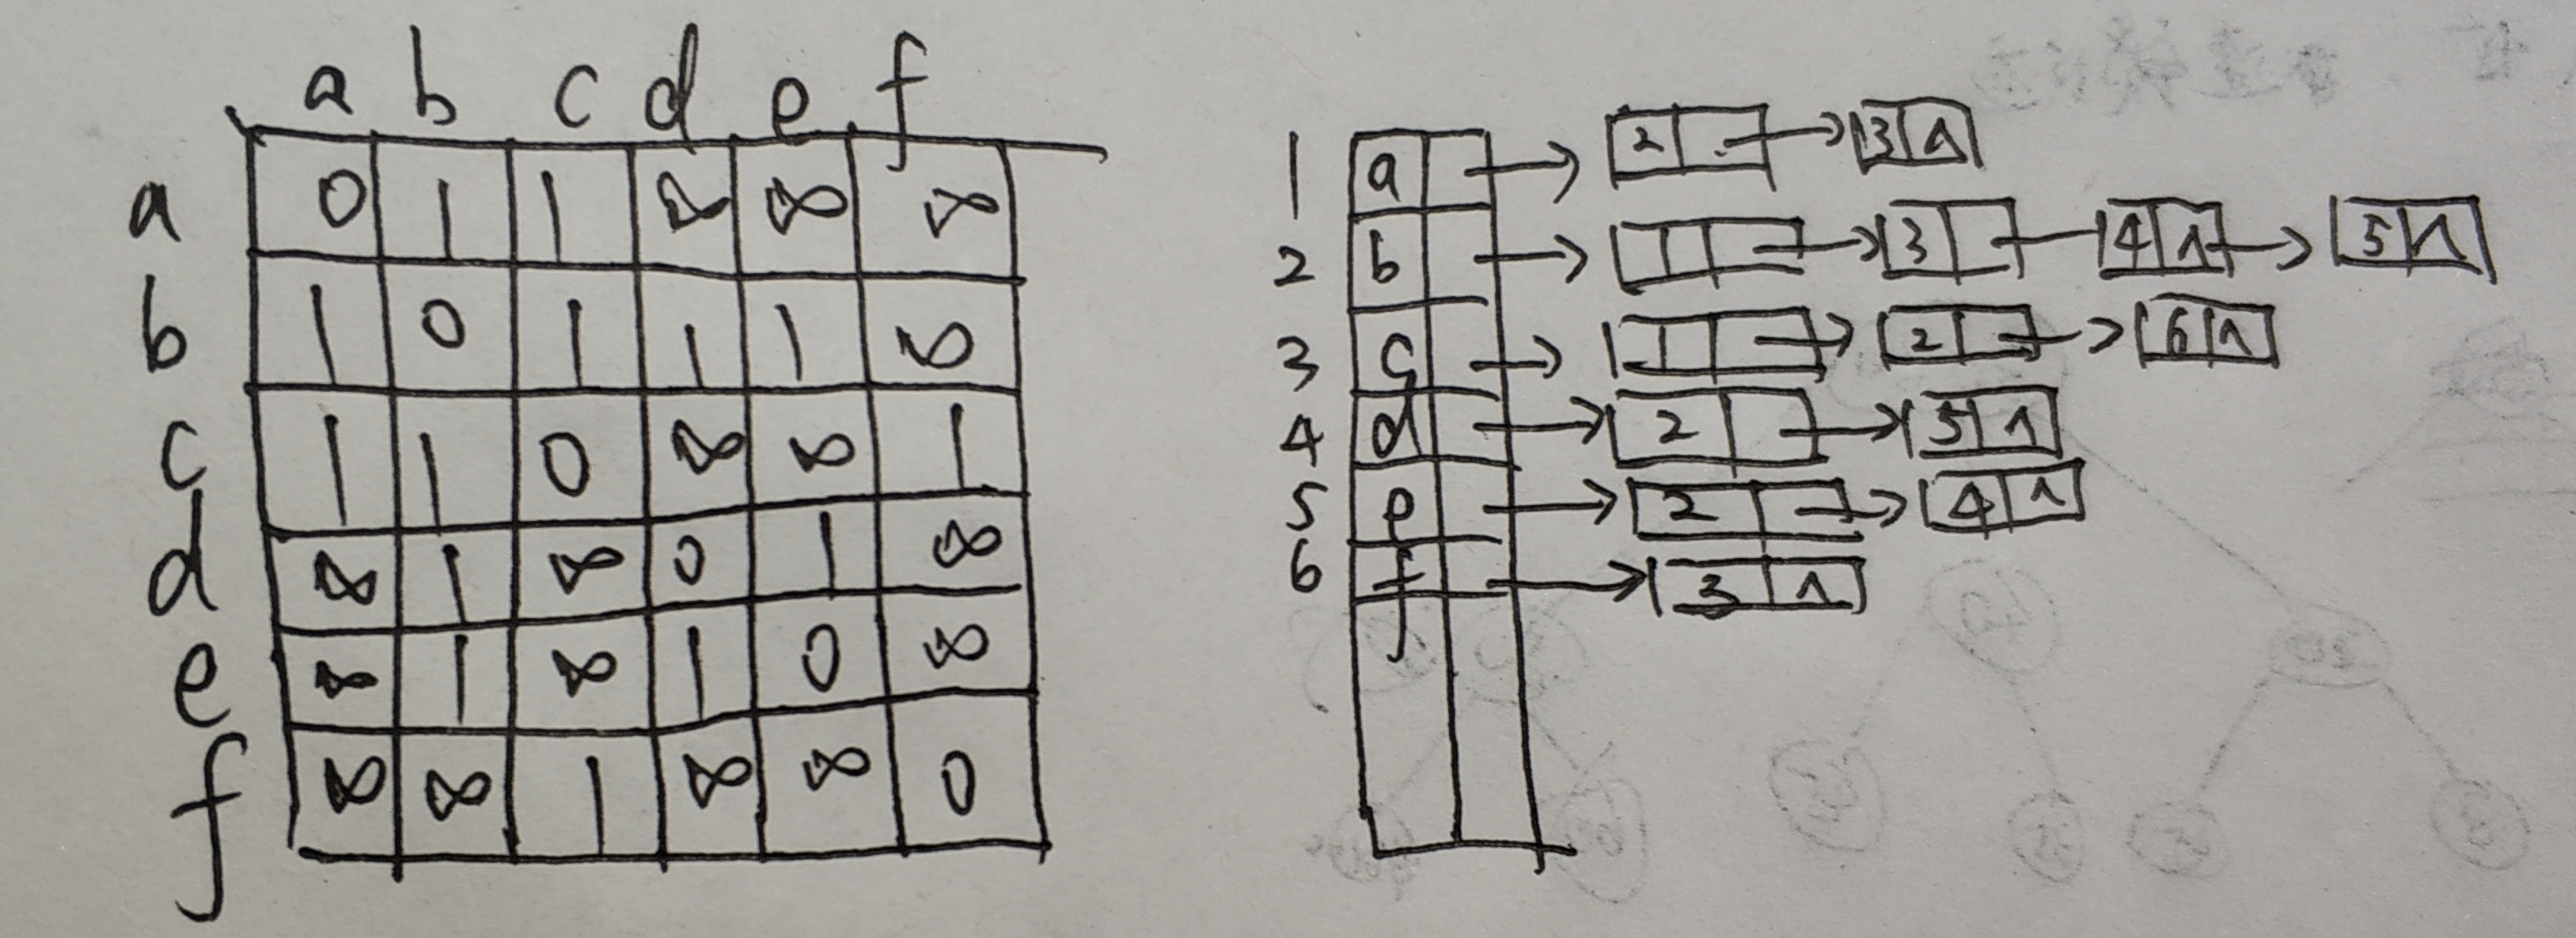
\includegraphics[scale=0.1]{example/chapter5/IMG_20181128_134745.png}
\end{figure} % 最小生成树
%%# -*- coding: utf-8-unix -*-
%%==================================================
\chapter{B+-树}
\label{chap6}
\begin{itemize}[noitemsep,topsep=0pt,parsep=0pt,partopsep=0pt]
	\item 知识点:讲解相关知识点。
	\item 题型:直接上真题。
\end{itemize}

\section{知识点和方法论}

\subsection{知识点}
\begin{itemize}[noitemsep,topsep=0pt,parsep=0pt,partopsep=0pt]
	\item B树就是二叉搜索树
	\item B-树多路搜索树m阶
	\begin{itemize}[noitemsep,topsep=0pt,parsep=0pt,partopsep=0pt]
			\item 即平衡m叉查找树
			\item 要求所有的叶节点在同一层
			\item 每个节点最多有m个分支,
			\item 每个节点的关键字个数的范围 $\left \lceil m/2 \right \rceil -1  \le n \le m-1 $
			\item 根节点的关键字个数     1<= n <=m-1 
			\item 根节点最少有2个分支
			\item 非根非叶节点最少有 $\left \lceil m/2 \right \rceil$  分支,比如三阶节点最少有2个分支
			\item B 树的叶节点数 = 是所有非叶结点个数+1
	\end{itemize}
	\item 2-3 B-树 其每个非叶节点都有两个或三个子女,而且所有叶都在统一层上
	\item B+ 树
	\begin{itemize}[noitemsep,topsep=0pt,parsep=0pt,partopsep=0pt]
		\item n个关键字的节点有n个分支
		\item 每个节点的关键字的个数 n 的取值范围    向上取整(m/2) <= n <=m
        \item 根节点的关键字个数取值范围为2 <= n <=m,
	\end{itemize}
\end{itemize}
\subsection{方法论}
\begin{itemize}[noitemsep,topsep=0pt,parsep=0pt,partopsep=0pt]
	\item B-插入节点
	\begin{itemize}[noitemsep,topsep=0pt,parsep=0pt,partopsep=0pt]
	    \item 求节点中关键字个数的范围  3阶  1 ~ 2
		\item 中间一个节点上升即可,递归上升; 比如 有三个节点中间的节点上升
	\end{itemize}
	\item B-树删除操作
	\begin{itemize}[noitemsep,topsep=0pt,parsep=0pt,partopsep=0pt]
			\item 如果终端节点 > [向上取整(m/2)-1],可以直接删除
			\item 	如果终端节点数 = [向上取整(m/2)-1],但是左右兄弟中节点会> [向上取整(m/2)-1],向兄弟借节点,就像流水一样,或者叫队列
			\begin{figure}[H]
				\centering  % 环境中的内容居中排版
				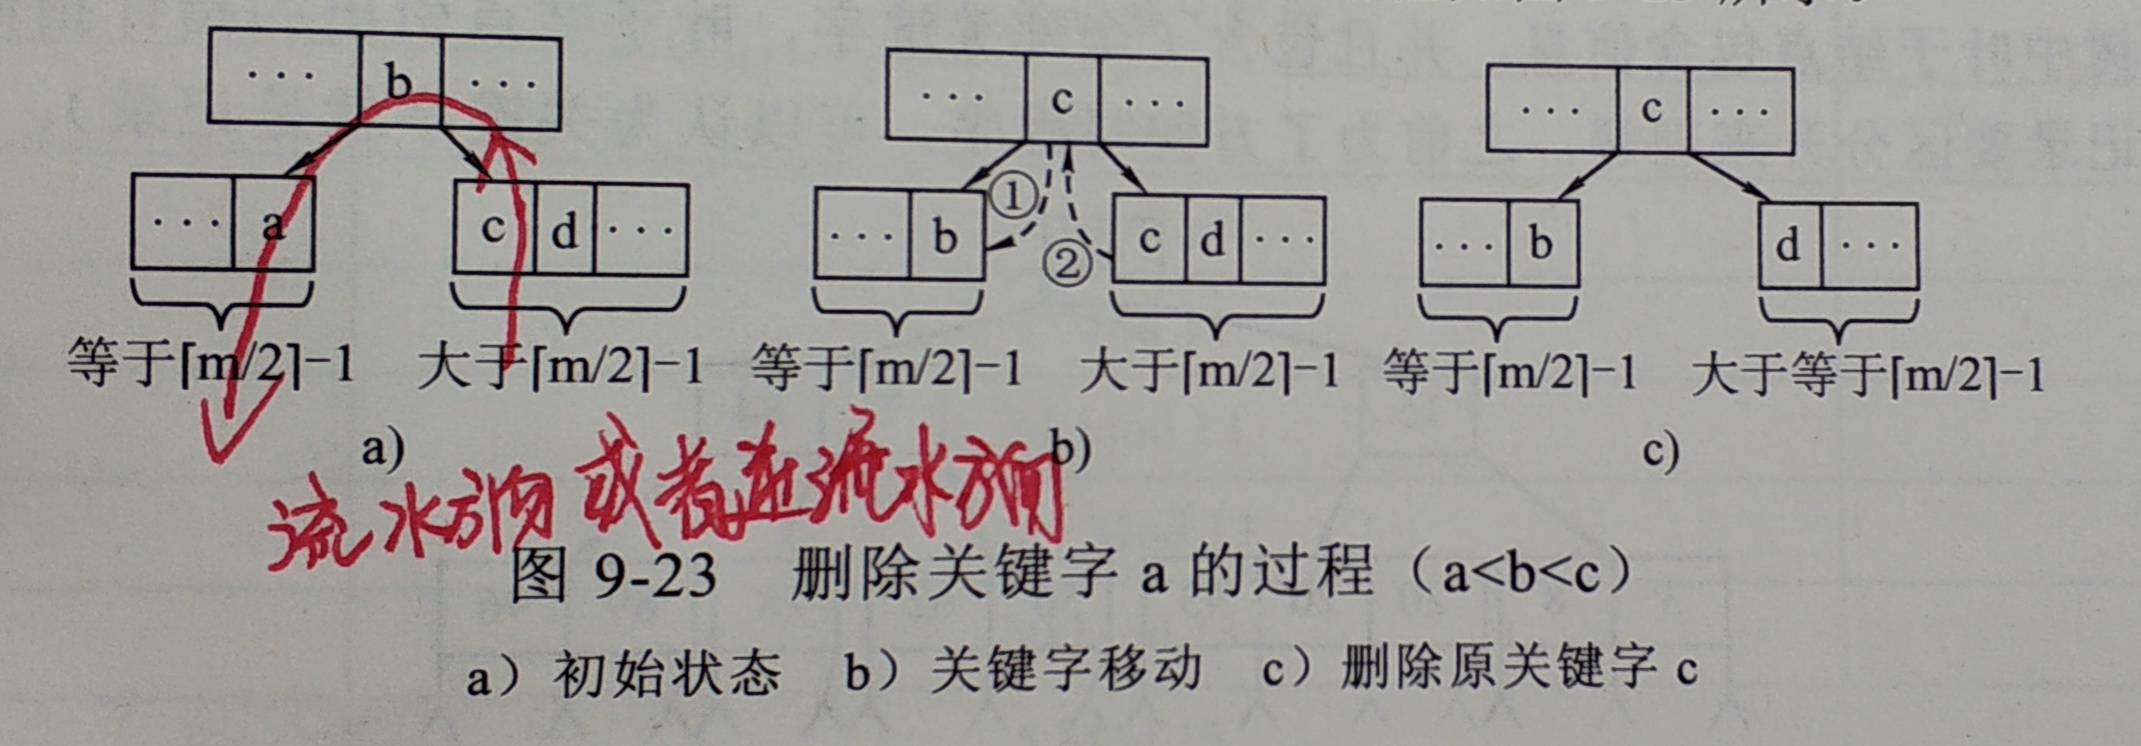
\includegraphics[scale=0.1]{example/chapter6/IMG_20181127_192544.png}
			\end{figure}

			\item 如果不在终端节点上,要替换替换到终端节点上
			\item 如果左右节点都是最少节点,则要掉下来一个,{\color{red}逆上升过程}

			\begin{figure}[H]
				\centering  % 环境中的内容居中排版
				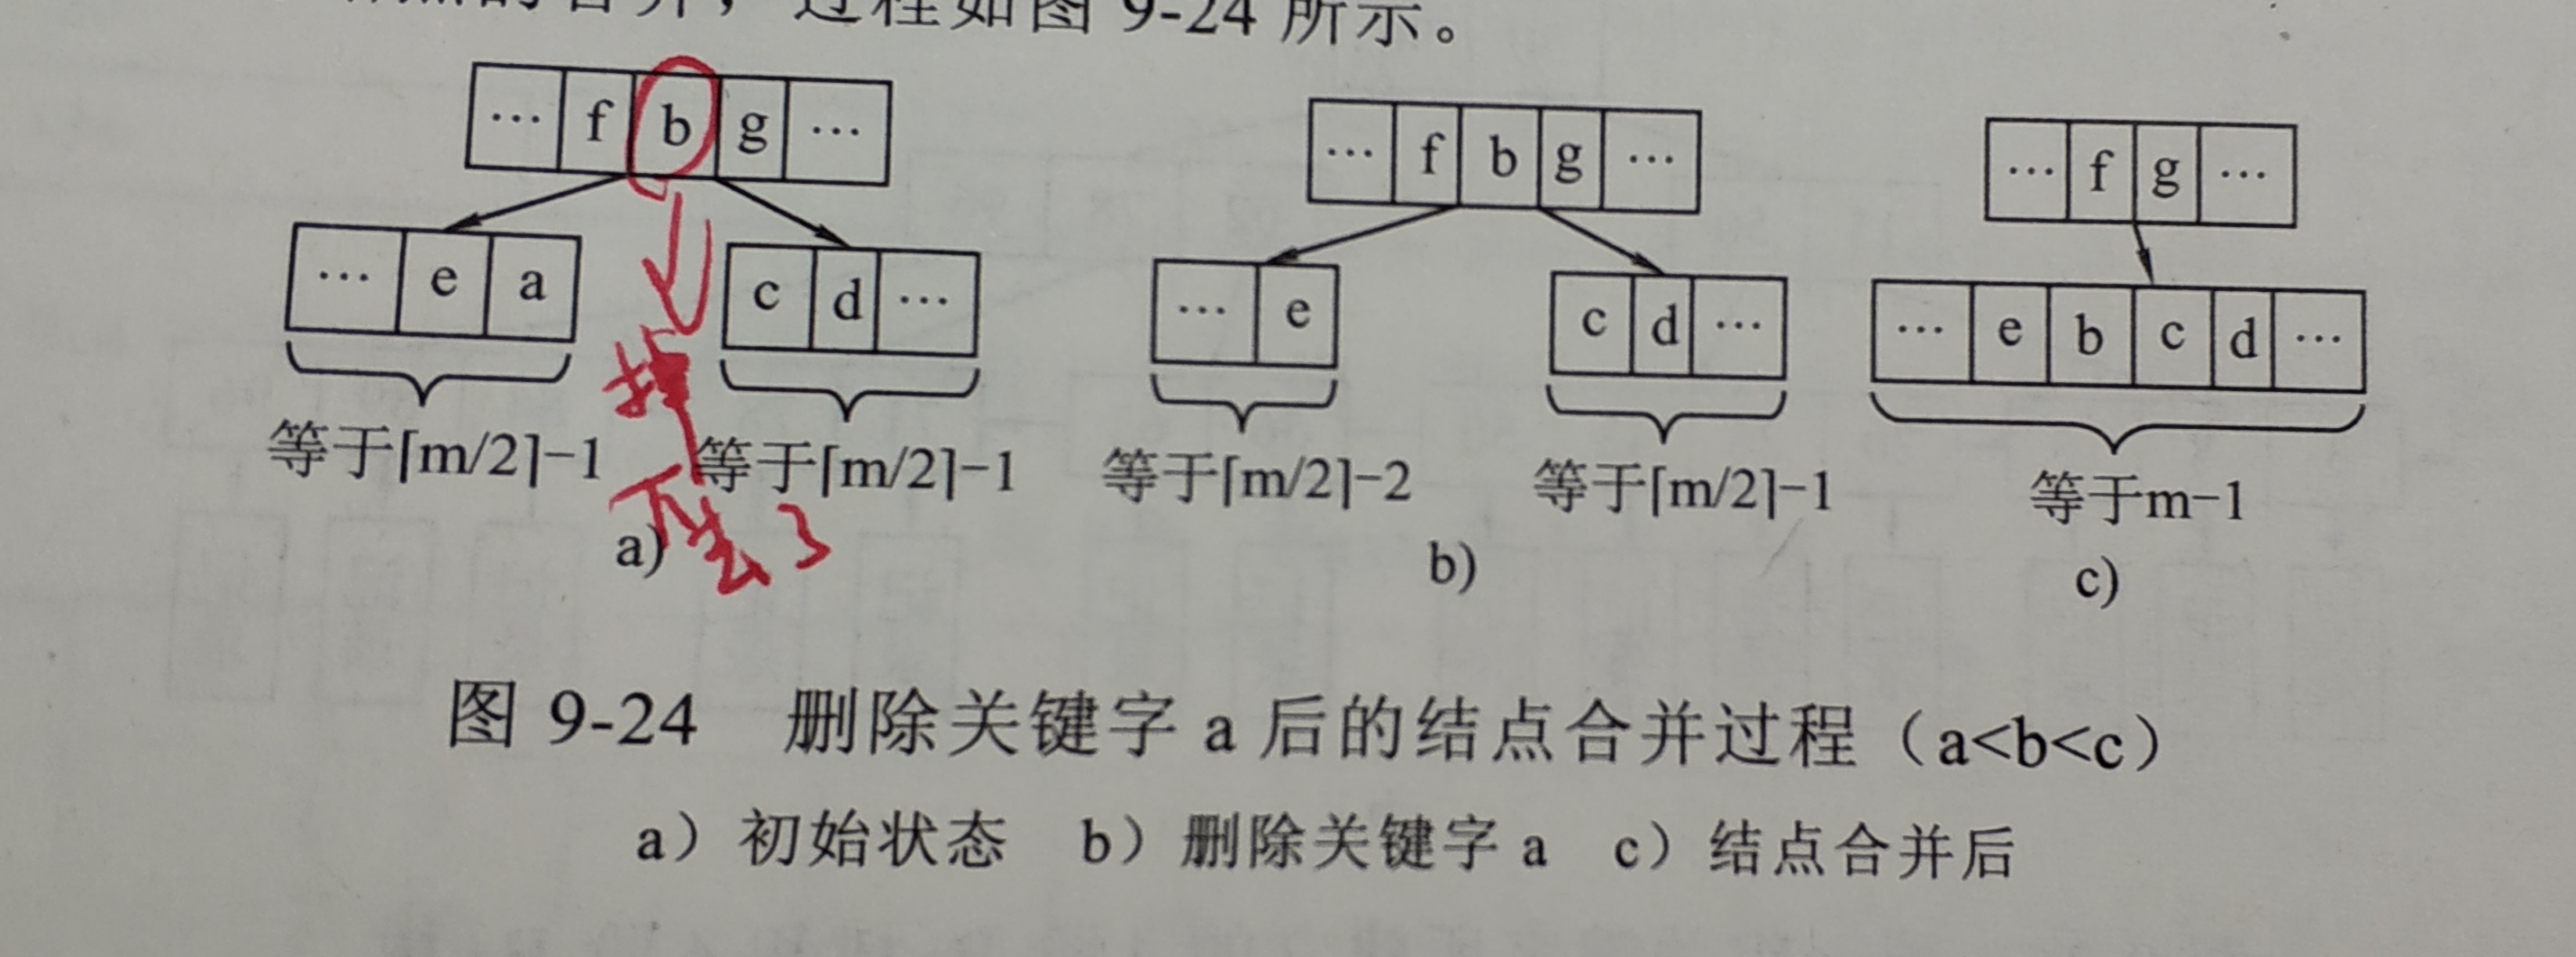
\includegraphics[scale=0.1]{example/chapter6/IMG_20181127_193515.png}
			\end{figure}
	\end{itemize}
\end{itemize}

\section{真题实战}


\subsection{2017年第(4)题}

\begin{lstlisting}[basicstyle=\small\ttfamily, caption={}, numbers=none]
对下面的3阶B-树,一次执行下列操作,画出各步操作的结果
1)插入90 2)插入25 3)插入45  4)删除60  5)删除80
\end{lstlisting}
\begin{figure}[H]
	\centering  % 环境中的内容居中排版
	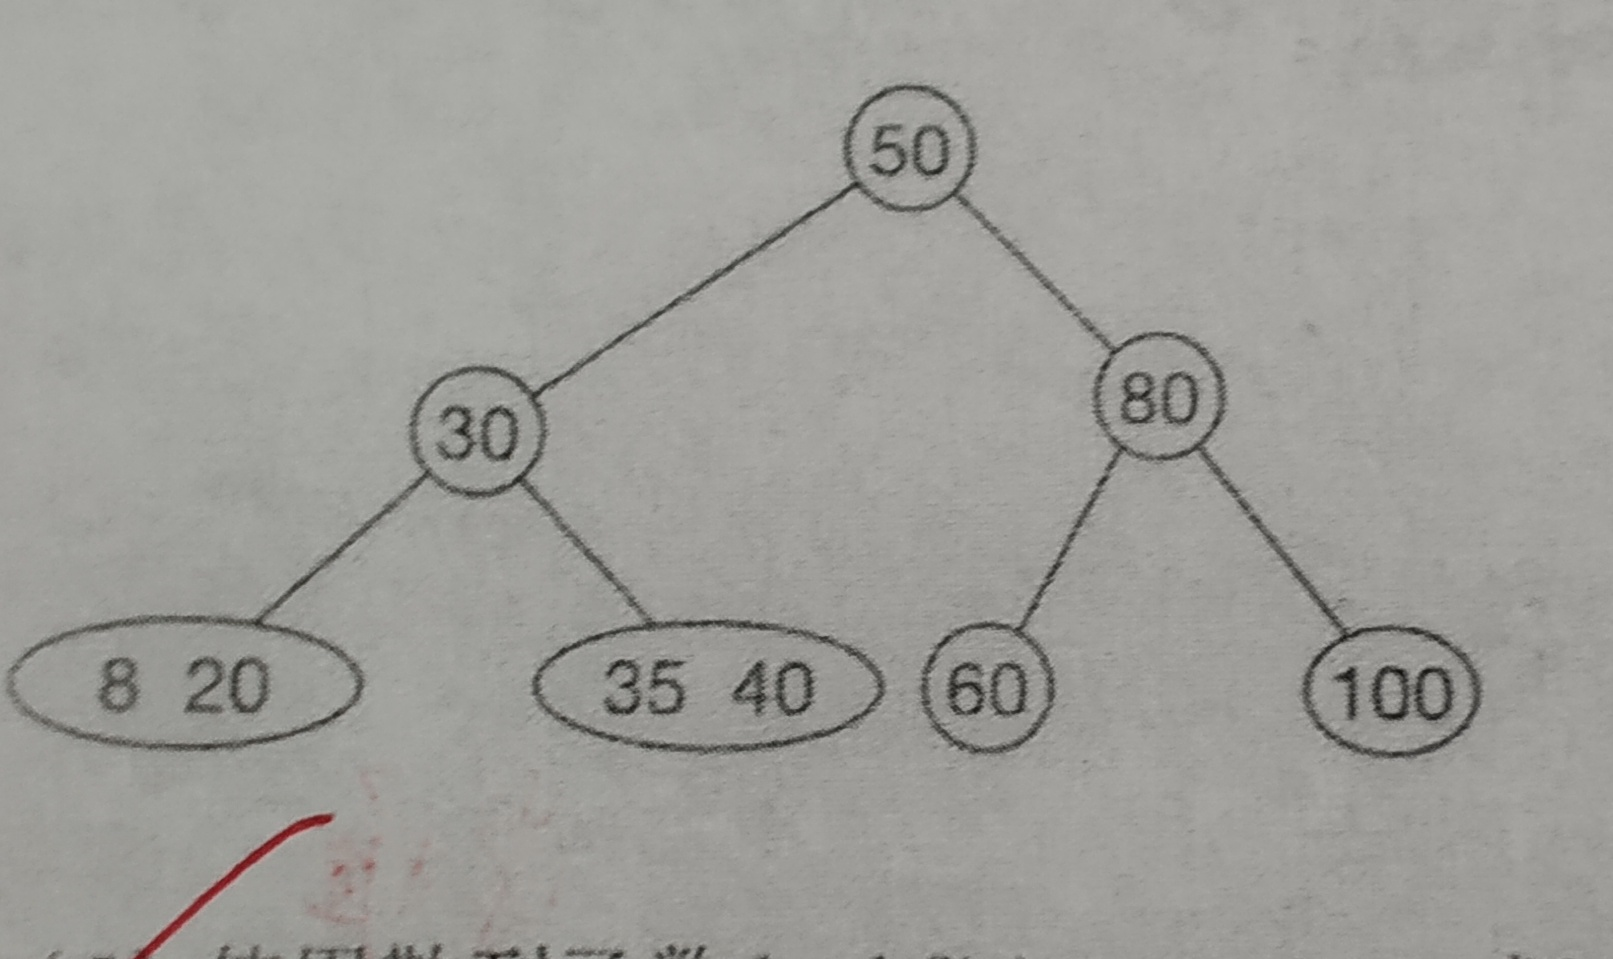
\includegraphics[scale=0.1]{example/chapter6/IMG_20181127_173638.png}
\end{figure}
解:\newline
\begin{figure}[H]
	\centering  % 环境中的内容居中排版
	\includegraphics[scale=0.1]{example/chapter6/IMG_20181127_200414.png}
\end{figure}


\subsection{2015年第(3)题}

\begin{figure}[H]
	\centering  % 环境中的内容居中排版
	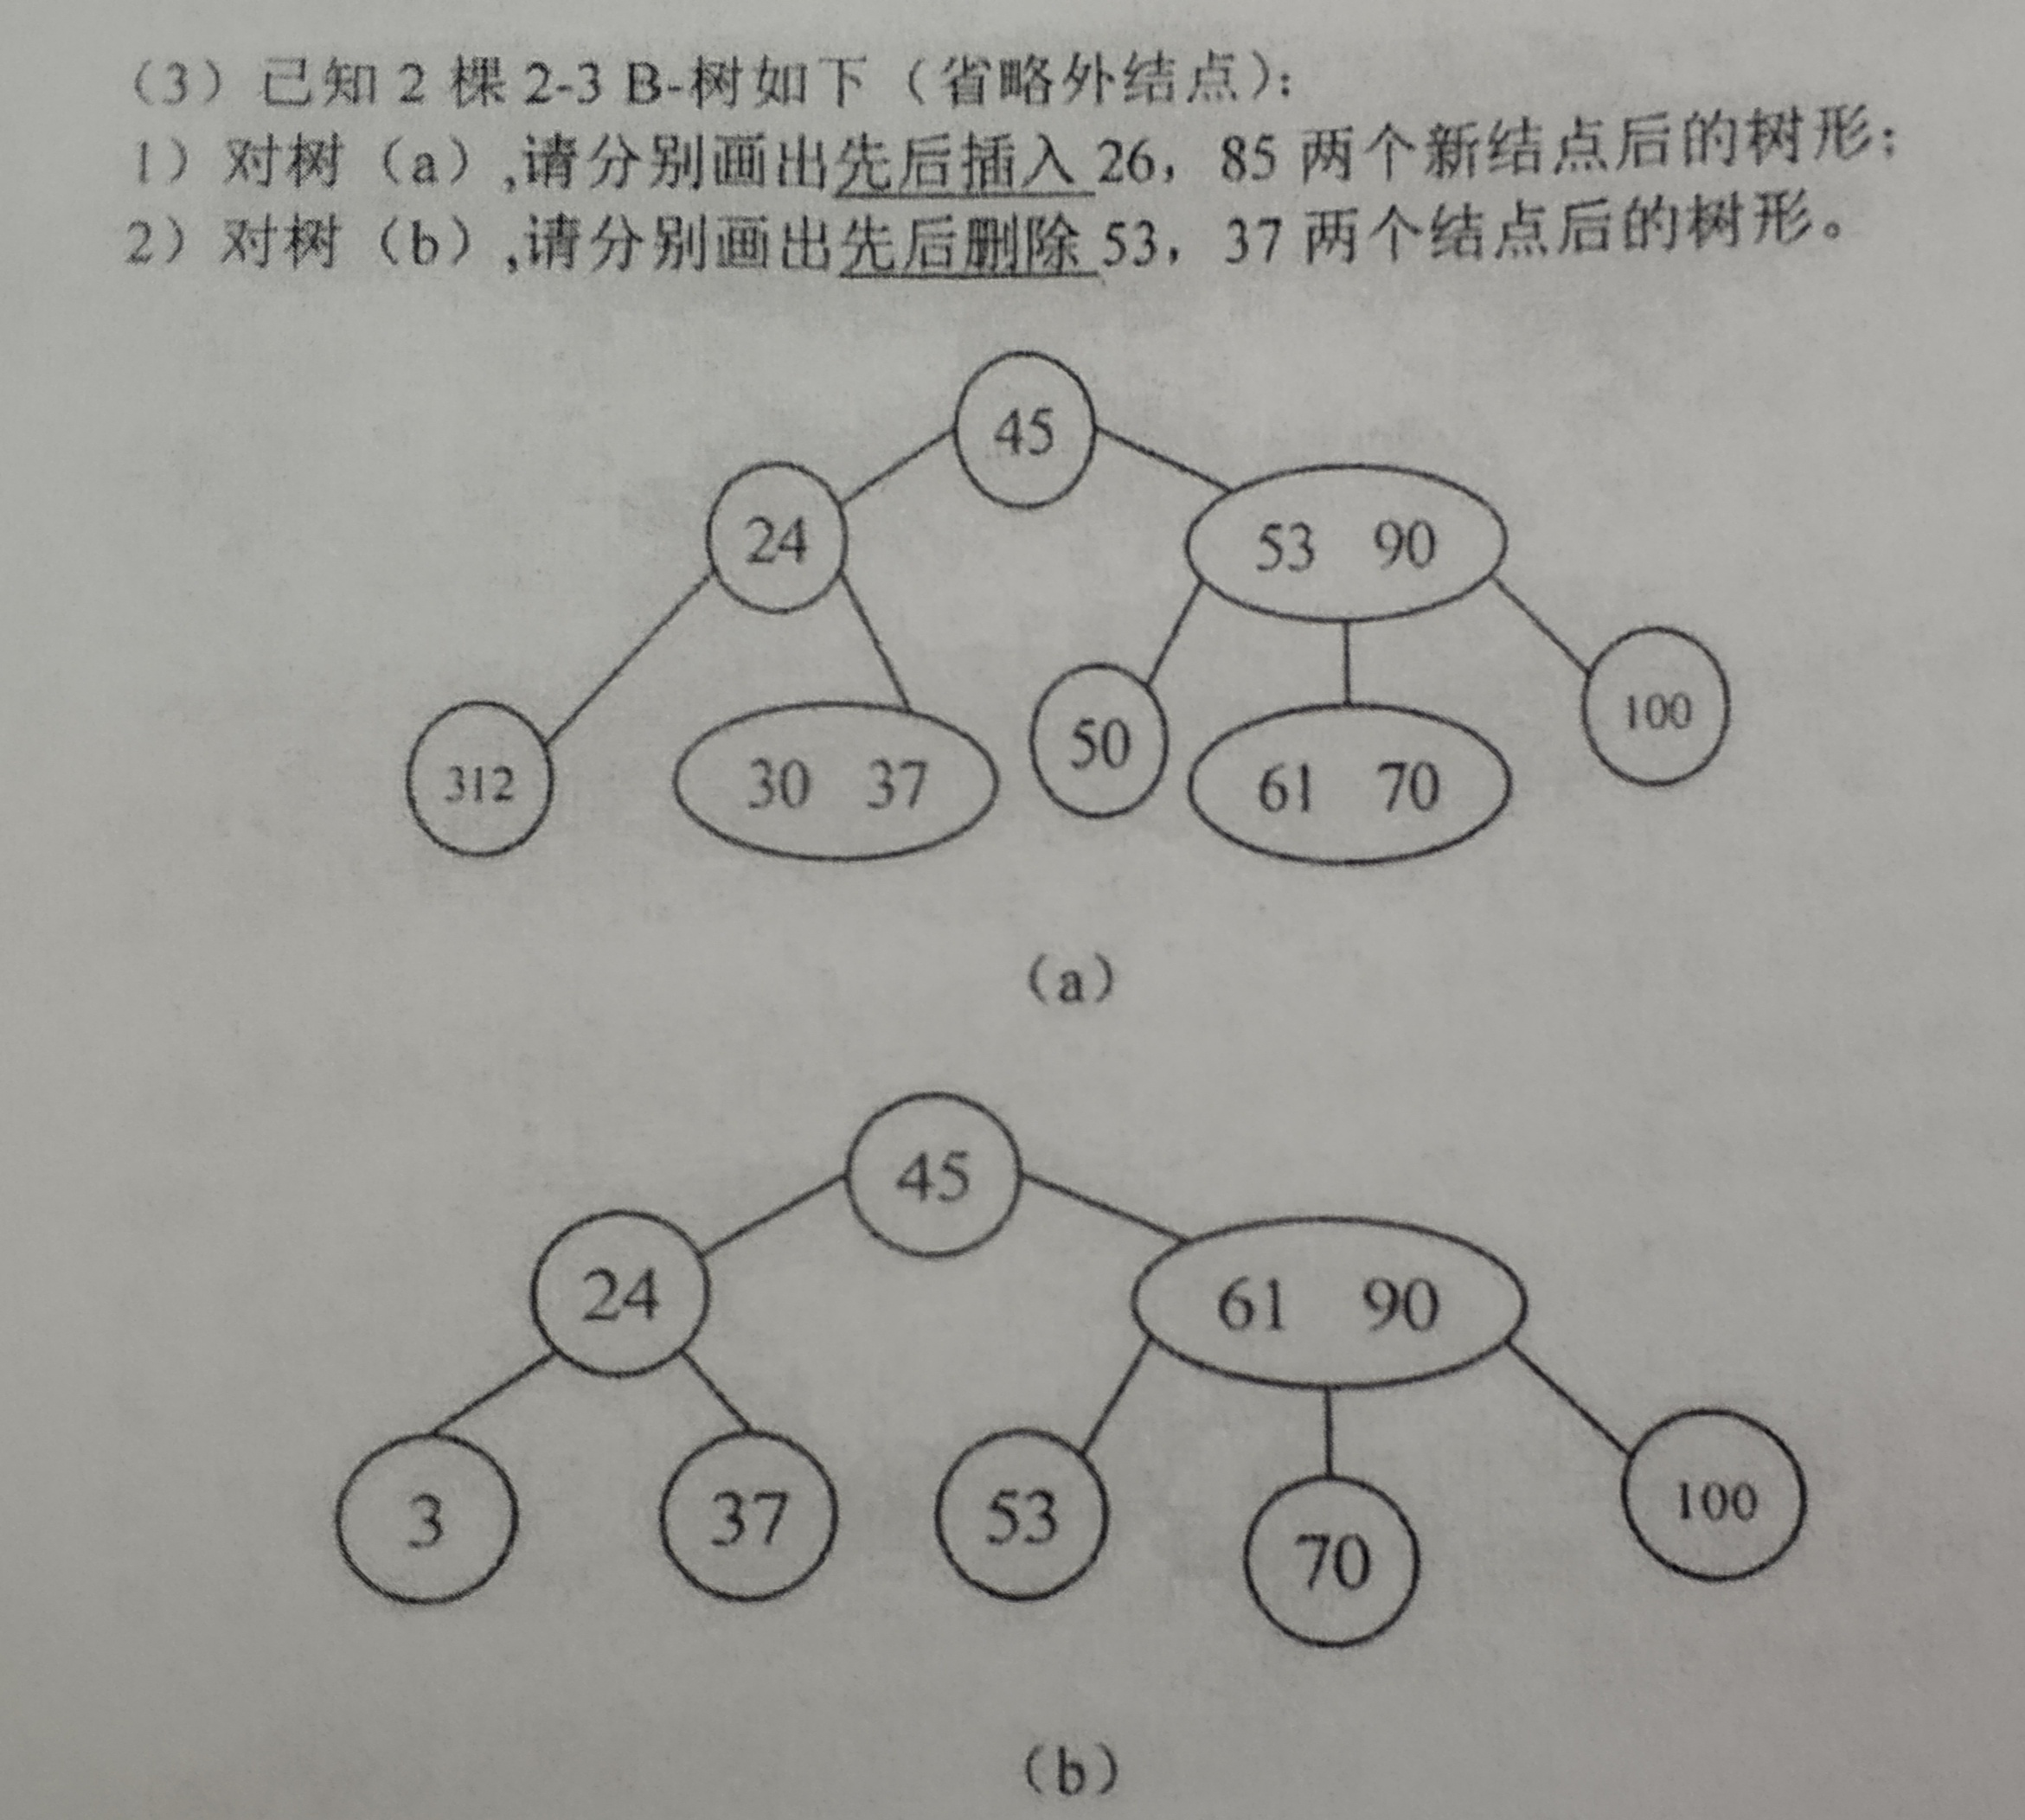
\includegraphics[scale=0.1]{example/chapter6/IMG_20181127_200601.png}
\end{figure}

解:\newline
\begin{figure}[H]
	\centering  % 环境中的内容居中排版
	\includegraphics[scale=0.1]{example/chapter6/IMG_20181127_202059.png}
\end{figure}

\subsection{2012年408}
已知一棵3阶B树,如下图所示。删除关键字78得到一棵新B树,其最右节点中的关键字是(  ).\newline
\begin{figure}[H]
	\centering  % 环境中的内容居中排版
	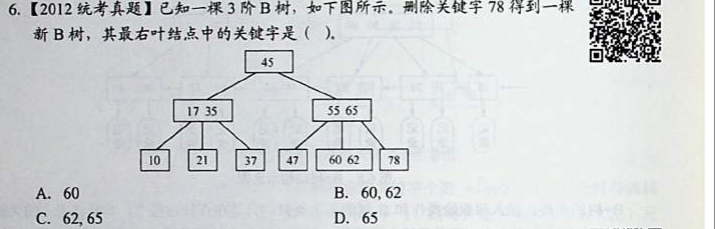
\includegraphics[scale=0.1]{example/chapter6/Annotation2019-09-25182756.png}
\end{figure}
解:\newline
B-树也满足一定的排序树的性质,一定要把握这一点。然后左边的节点足够借,然后就会像水流那样流动数据.\newline
\begin{figure}[H]
	\centering  % 环境中的内容居中排版
	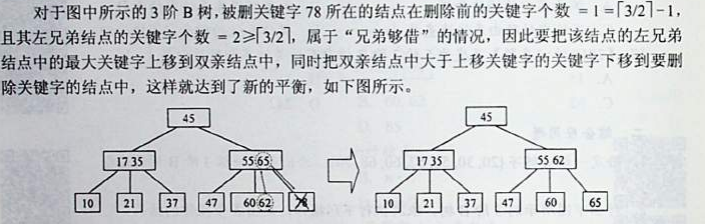
\includegraphics[scale=0.3]{example/chapter6/Annotation2019-09-25183110.png}
\end{figure}

\subsection{王道简单题}
高度为5的3阶B树至少有(  )个结点,至多有(   )个结点。\newline
A. 32 B . 31 C.120 D. 121\newline
解:\newline
问结点数而不是关键字树。\newline
至少就相当于一棵满二叉树,$2^5 - 1 = 31$ 个结点。\newline
至多就相当于一棵满三叉树,$3^5 - 1 = 121$个结点。\newline
 % B+- 新增题目
%%# -*- coding: utf-8-unix -*-
%%==================================================

\chapter{AVL and BST}
\label{chap7}

\begin{itemize}[noitemsep,topsep=0pt,parsep=0pt,partopsep=0pt]
	\item 知识点:讲解相关知识点。
	\item 题型:直接上真题。
\end{itemize}

\section{知识点和方法论}

\subsection{知识点}
\begin{itemize}[noitemsep,topsep=0pt,parsep=0pt,partopsep=0pt]
	\item 二叉平衡树 BST, 所有$\mbox{左孩子} \le \mbox{根结点} \le \mbox{右孩子}$
	\item 二叉排序树 AVL,也是一棵BST树,也满足BST的相关性质。
	\begin{itemize}[noitemsep,topsep=0pt,parsep=0pt,partopsep=0pt]
		\item 平衡因子的计算 $ \mbox{平衡因子} = \mbox{左子树的高度} - \mbox{右子树的高度} $
		\item 以平衡因子绝对值大于1的节点作为根节点
	\end{itemize}
\end{itemize}

\subsection{方法论}
\begin{itemize}[noitemsep,topsep=0pt,parsep=0pt,partopsep=0pt]
	\item 平衡二叉树的插入节点方法
	\begin{itemize}[noitemsep,topsep=0pt,parsep=0pt,partopsep=0pt]
		\item 圈出三个不平衡的节点,然后按照 小 中 大 的顺序,重新排列即可.可能还要移动一些元素配合移动。{\color{red}靠近最大不平衡的三个节点}.
		\item LL平衡旋转({\color{red}右单旋转}),由于在节点A的左孩子({\color{red}L})的左子树({\color{red}L})上插入了新结点,A失去平衡。向右转一下,即可。
		\item RR平衡旋转({\color{red}左单旋转}),由于在节点A的右孩子(R)的右子树(R)上插入了新节点,A的平衡因子由-1减至-2,导致以A为根的子树失去平衡,需要一次向左的旋转操作。
		\item LR平衡旋转(先左后右双旋转)。由于在A的左孩子(L)的右子树(R)上插入新结点,A的平衡因子由1增至2,导致以A为根的子树失去平衡,需要进行两次旋转操作,先左旋后右旋。
		\item RL 平衡旋转(先右后左双旋转)。由于在A的右孩子(R)的左子树(L)上插入新结点,A的平衡因子由-1减至-2,导致以A为根的子树失去平衡,先右旋,再左旋。
		\item 参考视频连接 \url{https://www.bilibili.com/video/av14273075/?p=2}
	\end{itemize}
\end{itemize}

\section{真题实战}


\subsection{2017年第5题}

\begin{lstlisting}[basicstyle=\small\ttfamily, caption={}, numbers=none]
5. 设数据元素的关键字序列为(20,30,15,45,78,65,25,60)依次插入这些元素,创建一颗平衡的二叉排序树(AVL树),请逐一画出每插入一个元素后的AVL
树的形态。
\end{lstlisting}
解:\newline
\begin{figure}[H]
	\centering  % 环境中的内容居中排版
	\includegraphics[scale=0.1]{example/chapter7/2018-12-03_16-40-08_366.png}
\end{figure}

\subsection{2010年408}
在如题图所示的平衡二叉树中插入关键字48后得到一棵新平衡二叉树,在新平衡二叉树中,关键字37所在节点的左、右子节点中保存的关键字分别是(   )\newline
A. 13,48    B.24,48  C. 24,53   D. 24, 90\newline
\begin{figure}[H]
	\centering  % 环境中的内容居中排版
	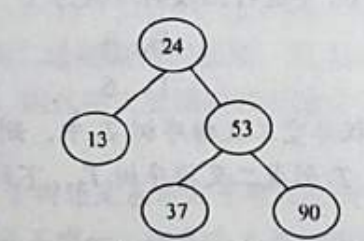
\includegraphics[scale=0.1]{example/chapter7/Annotation2019-09-24152618.png}
\end{figure}
解:\newline
\begin{figure}[H]
	\centering  % 环境中的内容居中排版
	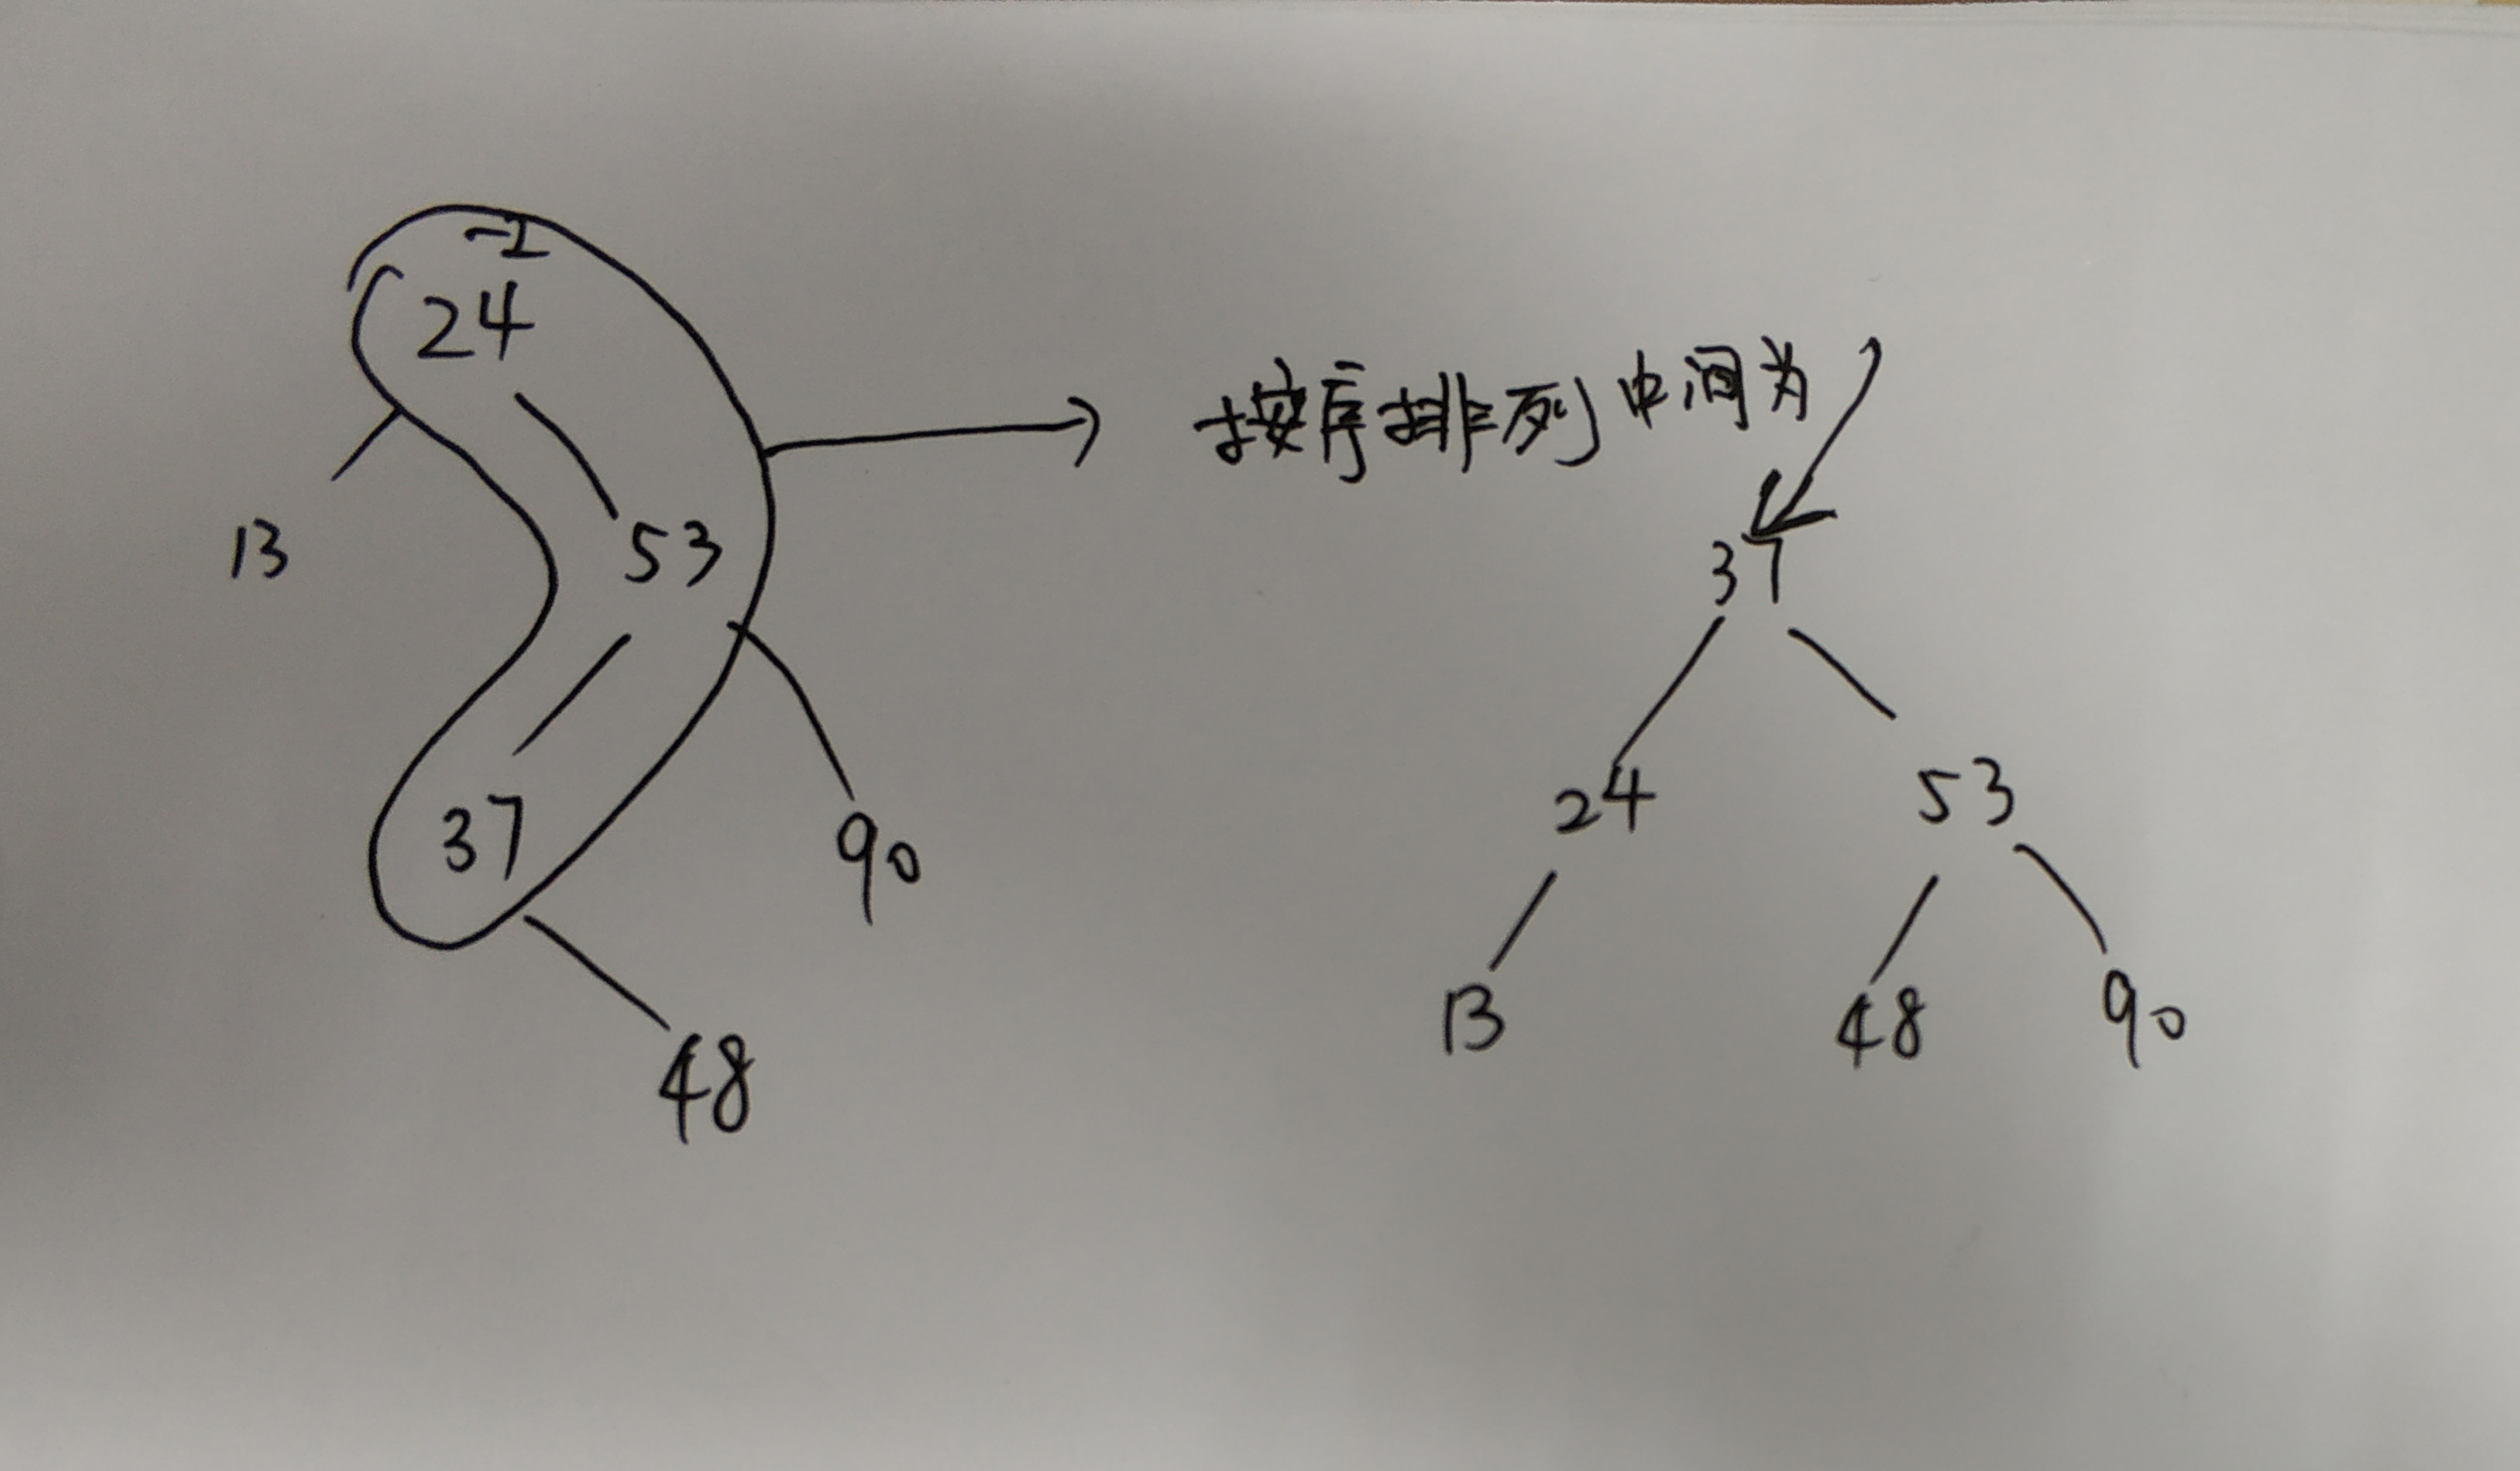
\includegraphics[scale=0.1]{example/chapter7/QQ20190923230023.jpg}
\end{figure}

\subsection{2013年408}
若将关键字1,2,3,4,5,6,7依次插入的初始为空的平衡二叉树T中,则T中平衡因子为0的分支节点的个数是(   )\newline
A. 0   B. 1  C. 2  D. 3
解:\newline
D.3个。
\begin{figure}[H]
	\centering  % 环境中的内容居中排版
	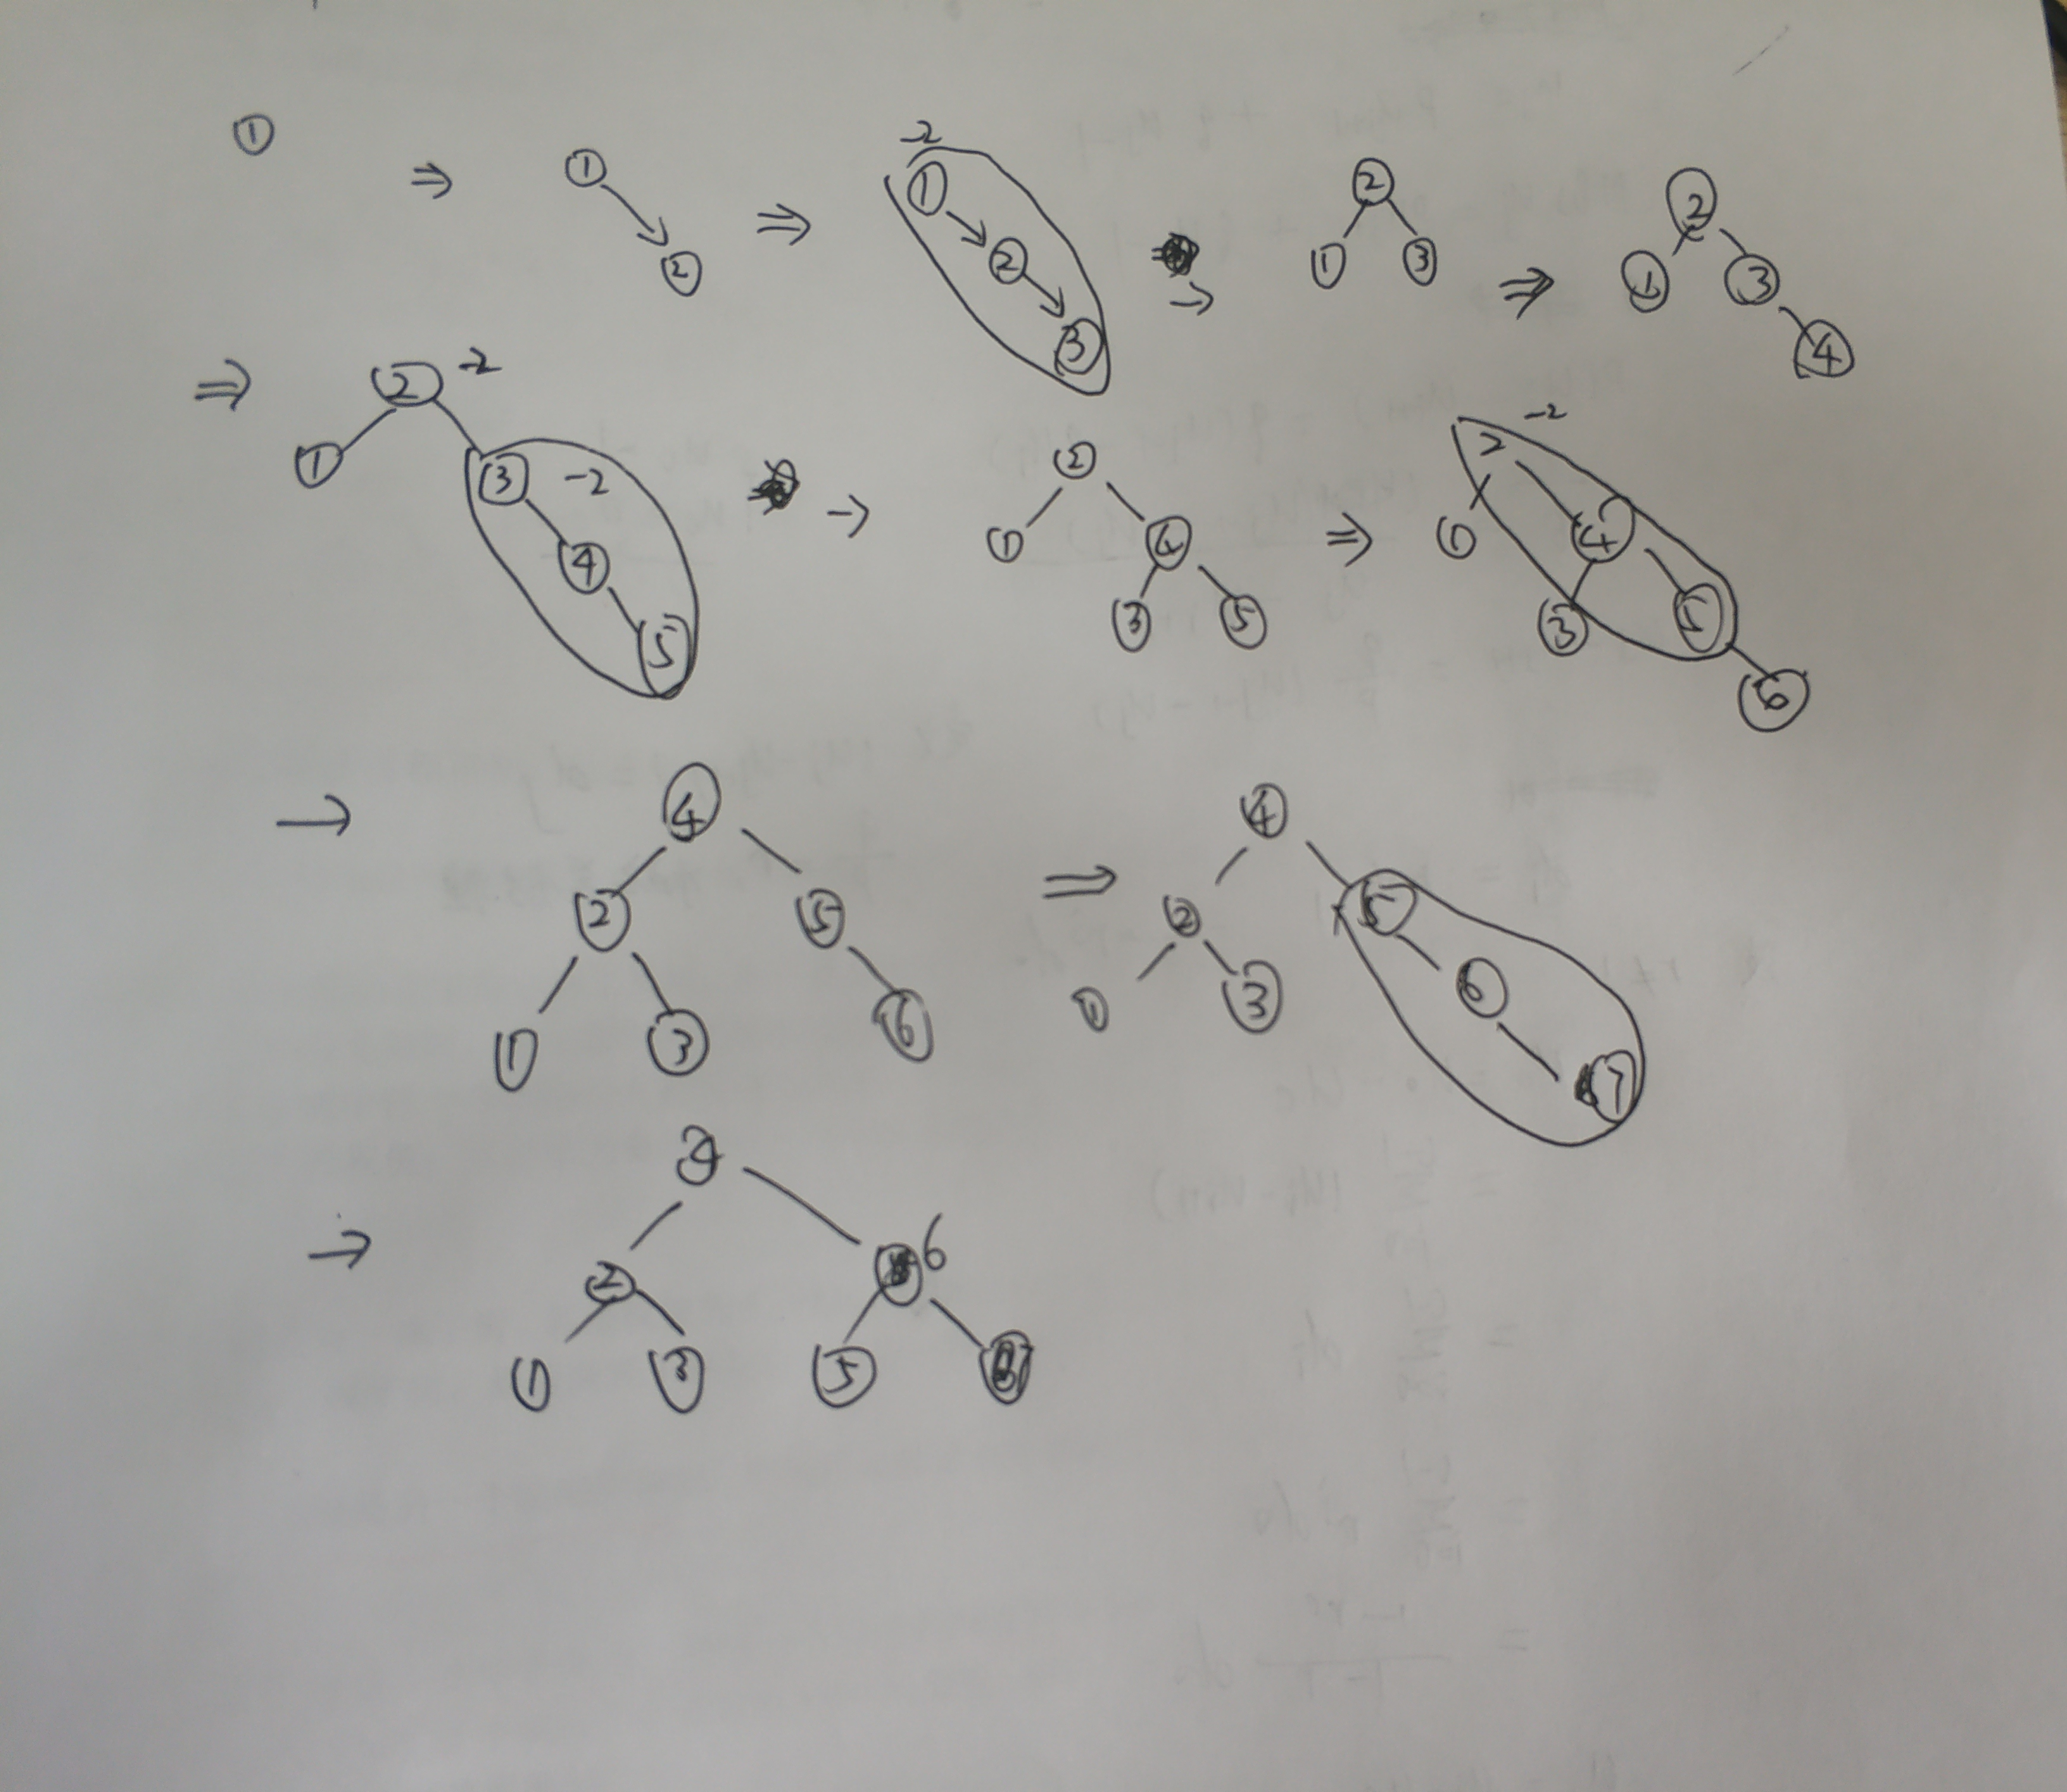
\includegraphics[scale=0.1]{example/chapter7/QQ20190924154030.jpg}
\end{figure}




 % 平衡二叉树 二叉排序树
%%# -*- coding: utf-8-unix -*-
%%==================================================

\chapter{AOV and AOE and BFS and DFS and Floyd}
\label{chap8}

\begin{itemize}[noitemsep,topsep=0pt,parsep=0pt,partopsep=0pt]
	\item 知识点:讲解相关知识点。
	\item 题型:直接上真题。
\end{itemize}

\section{知识点和方法论}

\subsection{知识点}
\begin{itemize}[noitemsep,topsep=0pt,parsep=0pt,partopsep=0pt]
	\item AOV activity on vertex
	\item AOE activity on edge
	\item 核心:广度优先遍历和深度优先遍历
	\item 图的表示方法,邻接矩阵法和链表法
	\item 图的广度优先遍历和二叉树的层序遍历完全一致。
	\item 图的广度优先遍历的时间复杂度是O(n+e) 
\end{itemize}

\subsection{方法论}

\begin{itemize}[noitemsep,topsep=0pt,parsep=0pt,partopsep=0pt]
	\item 关键路径计算相关
	\begin{itemize}[noitemsep,topsep=0pt,parsep=0pt,partopsep=0pt]
	\item 事件$V_{k}$的最早发生时间ve(k)的计算\newline
		$ve(\mbox{源头}) = 0$\newline
		ve(k)=Max\{ve(j)+Weight($v_{j}, v_{k}$)\},Weight($v_{j}$, $v_{k}$) 表示 <$v_j$,$v_k$> 的权值\newline
		{\color{red}在计算ve(k)时,是按从前往后的顺序来计算的}\newline
	\item 事件$V_{k}$的最迟发生时间vl(k)\newline
		$vl(\mbox{汇点})=ve(\mbox{汇点})$\newline
		vl(j) = Min\{vl(k)-Weight($v_j$,$v_k$)\}, Weight($v_j$, $v_k$)表示<$v_j$, $v_k$>上的权值\newline
		{\color{red}在计算vl(j)时,是按照从后往前的顺序来计算的。}\newline
	\item 活动$a_i$的最早开始时间e(i)\newline
	它是指该活动的{\color{red}起点}所表示的事件最早发生时间。如果边<$v_k,v_j$>表示活动$a_i$,则有e(i) = ve(k).\newline
	\item 活动$a_i$的最迟开始时间l(i)\newline
	它是指该活动的{\color{red}终点}所表示的事件最迟发生时间与该活动所需时间之差。如果边<$v_k,v_j$>表示活动$a_i$,则有l(i)= vl(j) - Wight($v_k, v_j$).\newline
	\item 一个活动$a_i$的最迟开始时间l(i)和其最早开始时间的e(i)的差值d(i) = l(i) - e(i) 
	\end{itemize}
	\item 求关键路劲的算法步骤如下:\newline
	(1) 求AOE网的所有事件的最早发生时间 ve() \newline
	(2) 求AOE网的所有事件的最迟发生事件 vl() \newline
	(3) 求AOE网中所有活动的最早开始时间 e() \newline
	(4) 求AOE网中所有活动的最迟开始时间 l() \newline
	(5) 求AOE网中所有活动的差额时间d(), 找出偶有d() = 0的活动构成关键路径。
\end{itemize}

\subsection{BFS算法思想}
\begin{lstlisting}[basicstyle=\small\ttfamily, caption={}, numbers=none]
void BFSTraverse(Graph G) {
	for (int i = 0; i < G.vexNum; i++) { // 访问数组初始化 
	visited[i] = false;
	}

	initQueue(Q); // 初始化辅助队列
	for (int i = 0; i < G.vexNum; i++) {
		if (!visited[i]) {
		BFS(G, i);
		}
	}
}

void BFS(Graph G, int v) {
	cout << "visit vex: " << G.vex[v] << endl;
	visited[v] = true;
	enQueue(Q, v);
	while (!isQueueEmpty(Q)) {
		deQueue(Q, v);
		for (int i = 0; i < G.vexNum; i++) {
			if (!visited[i] && G.edge[v][i] == 1) {  // 表示 v 和 顶点 I 是连通的
			cout << "visit vex2: " << G.vex[i] << endl;
			visited[i] = true;
			enQueue(Q, i);
			}
		}
	}
}
• 核心函数的简单记忆版本
○ void BFSTraverse(Graph G)
	§ 初始化 访问数组
	§ 初始化 队列
	§ 对每一个点调用BFS函数
		□ 如果没有访问过就调用BFS函数
○ void BFS(Graph G, int v)  // 参数图  和要访问的某个节点
	§ 访问要访问的节点
	§ 访问数组设为已经访问过
	§ 把这个节点加入到队列中
	§ 循环判断队列是否为空
		□ 如果为空结束访问;这个函数都结束了
		□ 不为空
			® 把队列中的那个元素弹出来放入v中
			® 遍历与这个点相连接的点,
				◊ 如果是连接的而且没有访问过
					} 那么访问他
					} 访问数组设为1
					} 把这个与之相连的点放入队列中
\end{lstlisting}


\subsection{DFS算法思想}
\begin{lstlisting}[basicstyle=\small\ttfamily, caption={}, numbers=none]
void DFSTraverse(Graph G) {
	for (int i = 0; i < G.vexNum; i++) {
		visited[i] = false;
	}
	for (int i = 0; i < G.vexNum; i++) {
		if (!visited[i]) {
			DFS(G, i);
		}
	}
}
void DFS(Graph G, int v) {
	cout << "visit vex: " << G.vex[v] << endl;
	visited[v] = true;
	for (int i = 0; i < G.vexNum; i++) {
	if (!visited[i] && G.edge[v][i] == 1) {  // 表示 v 和 顶点 I 是连通的
		DFS(G, i);
	}
}
• 两个核心函数背诵版
○ void DFSTraverse(Graph G) {
	§ 把 访问数组 初始化
	§ 从0点开始如果没有访问,调用DFS
○ void DFS(Graph G,int v)
	§ 访问v点
	从0点开始看和v点相连接的且没有访问过的点使用DFS
\end{lstlisting}

\section{真题实战}
\subsection{王道225页第8题}
\begin{figure}[H]
	\centering  % 环境中的内容居中排版
	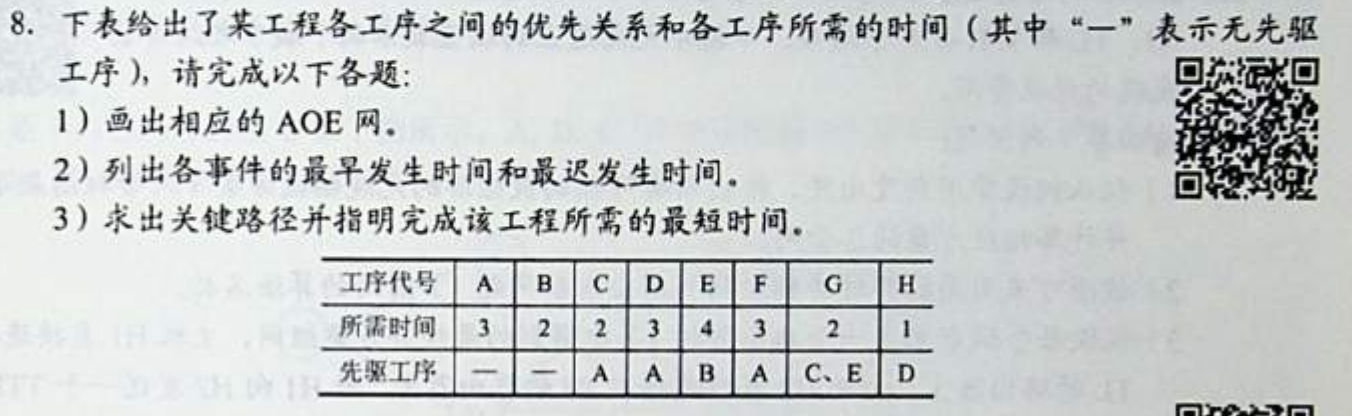
\includegraphics[scale=0.3]{example/chapter8/Annotation2019-08-23221311.png}
\end{figure}
解:\newline
\begin{figure}[H]
	\centering  % 环境中的内容居中排版
	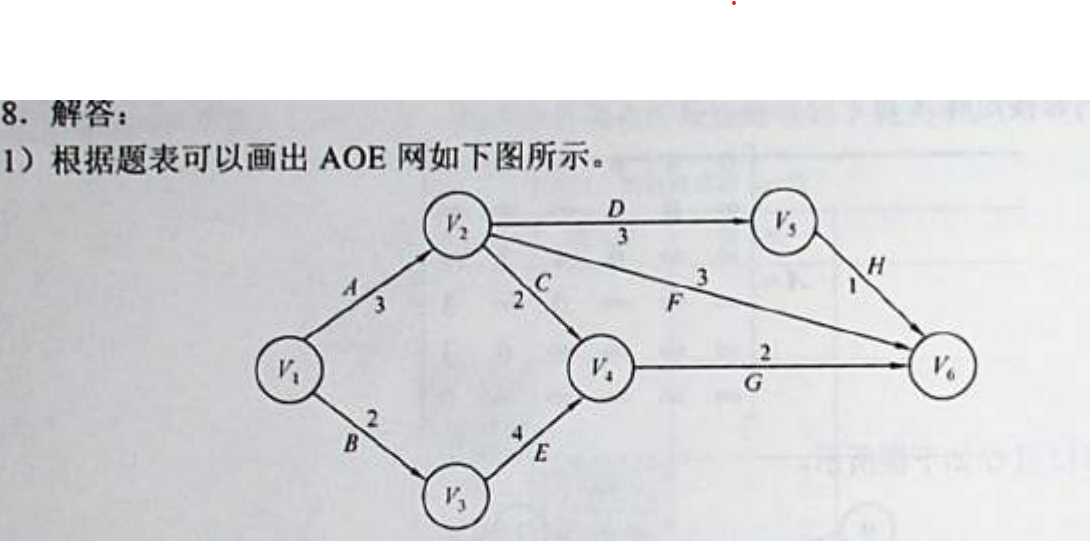
\includegraphics[scale=0.3]{example/chapter8/Annotation2019-08-24093946.png}
\end{figure}
注:\newline
这张图不是一下子就画出来的,可能需要画两遍,第一遍随性画出来。第二遍,合并顶点.\newline
箭头代表了计算方向\newline
\begin{figure}[H]
	\centering  % 环境中的内容居中排版
	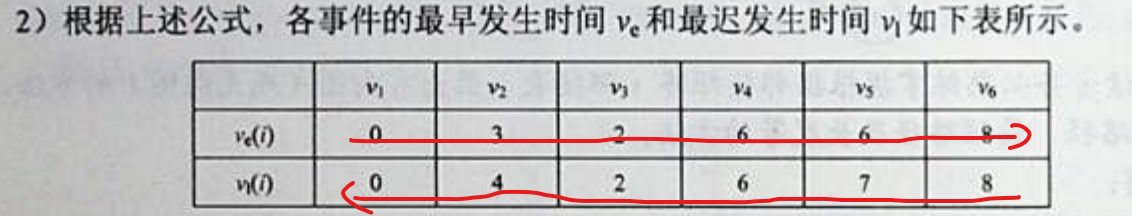
\includegraphics[scale=0.3]{example/chapter8/Annotation2019-08-24094509.png}
\end{figure}
\begin{figure}[H]
	\centering  % 环境中的内容居中排版
	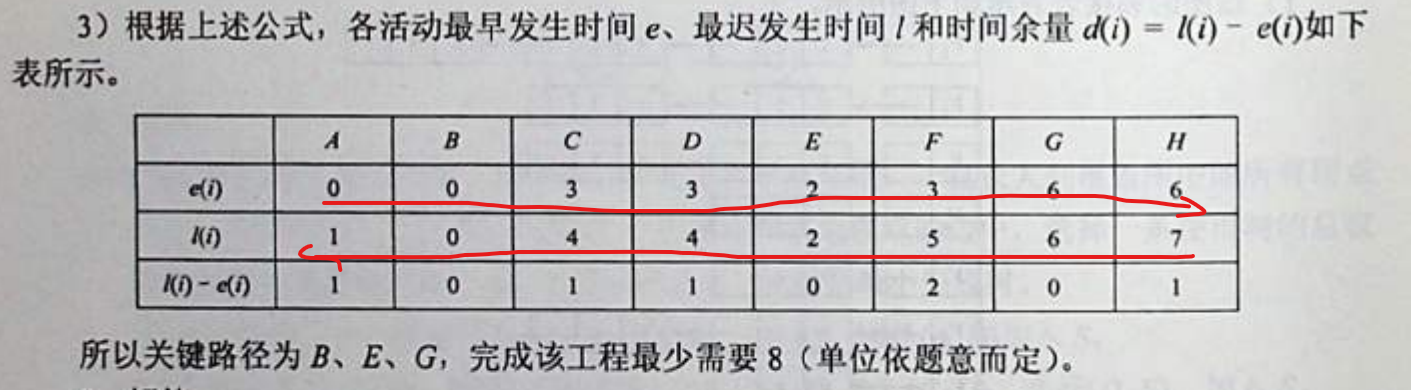
\includegraphics[scale=0.3]{example/chapter8/Annotation2019-08-24094705.png}
\end{figure}

\subsection{2015年408}
已知含有5个顶点的图G如下图所示.\newline
请回答下列问题:\newline
1) 写出图G的邻接矩阵A(行、列下标从0开始).\newline
2) 求$A^2$,矩阵$A^2$中位于0行3列元素值的含义是什么??\newline
3) 若已知具有n(n$\ge$2)个顶点的图的邻接矩阵为B,则$B^m (2\le m\le n)$中非零元素的含义是什么?\newline
\begin{figure}[H]
	\centering  % 环境中的内容居中排版
	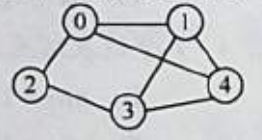
\includegraphics[scale=0.3]{example/chapter8/Annotation2019-09-25090123.png}
\end{figure}
解:\newline
1)\newline
A = 
\begin{bmatrix}
	 0 & 1 & 1 & 0 & 1 \\ 
	 1 & 0 & 0 & 1 & 1 \\
	 1 & 0 & 0 & 1 & 0 \\
	 0 & 1 & 1 & 0 & 1\\
	 1 & 1 & 0 & 1 & 0 
\end{bmatrix}\quad
2)\newline
$A^2 = $
\begin{bmatrix}
	3 & 1 & 0 & 3 & 1 \\ 
	1 & 3 & 2 & 1 & 2 \\
	0 & 2 & 2 & 0 & 2 \\
	3 & 1 & 0 & 3 & 1\\
	1 & 2 & 2 & 1 & 3 
\end{bmatrix}\quad
表示:\newline
0行3列的元素值3表示从顶点0到顶点3之间长度为2的路径共3条\newline
3)\newline
表示:途中从顶点i到顶点j长度为n的路径条数。\newline

\subsection{PAT Floyd算法}
\url{https://www.nowcoder.com/pat/5/problem/4306}
题目描述:\newline
微博被称为Twitter的中文版。 微博上的一个用户可能有很多关注者,也可能关注许多其他用户。 因此,形成了具有追随者关系的社交网络。 当用户在微博上发布帖子时,他/她的所有关注者都可以查看并转发他/她的帖子,然后他们的关注者可以再次转发。 现在给定一个社交网络,假设只计算了L级间接关注者,则应该计算任何特定用户的最大潜在转发量。\newline
输入描述:\newline
对于每种情况,第一行包含2个正整数:N(<= 1000),用户数; L(<= 6),是间接关注者的级别数。 \newline
因此,假定所有用户的编号都从1到N。然后是N行,每行的格式为:\newline
M [i]个用户列表[i]
其中M [i](<= 100)是用户[i]跟随的总人数; user\_list [i]是M [i]个用户的列表,后跟user [i]。 保证没有人可以跟随自己。 所有数字都用空格分隔。
然后,最后给出一个正数K,后跟K个用户ID进行查询。\newline
输出描述:\newline
对于每个UserID,您应该在一行中打印出该用户可以触发的最大潜在转发量,假设可以查看初始帖子的每个人都将转发一次,并且仅计算L级间接关注者。\newline
\begin{lstlisting}[basicstyle=\small\ttfamily, caption={}, numbers=none]
思路:抄大神写的弗洛伊德算法 求任意两点之间的最短距离 加了注释
教科书般的 Floyd算法。
#include <cstdio>
#include <cstring>
#include <string>
#include <iostream>
#include <fstream>
using namespace std;
#ifndef debug
ifstream ifile("case.txt");
#define cin ifile
#endif
 
 
int f[1024][1024];
void better(int &x, int y)
{
    if ((x < 0) || (x > y))
    {
        x = y;
    }
}
 
 
int main() {
    int n, m;
    cin >> n >> m;
    memset(f, 0xff, sizeof(f));
    for (int i = 1; i <= n; i++)
    {
        int j;
        for (cin >> j; j; --j)
        {
            int x;
            cin >> x;
            f[x][i] = 1;// x 点和 i 点的距离是1
        }
    }
    for (int k = 1; k <= n; ++k)
    {
        for (int i = 1; i <= n; ++i)
        {
            if (f[i][k] >= 0)
            {
                for (int j = 1; j <= n; ++j)
                {
                    if (f[k][j] >= 0)
                    {
                        better(f[i][j], f[i][k] + f[k][j]);// 如果 i j 两点的距离比 i K
                                                           // 和 k j之间的距离大就改变这i 和 j 之间距离大小
                    }
                }
                 
            }
        }
    }
 
    int x;
 
    for (cin >> x; x; --x)
    {
        int y;
        cin >> y;
        int z = 0;
        for (int i = 1; i <= n; ++i)
        {
            if ((i != y) && (f[y][i] >= 0) && (f[y][i] <= m))// 如果 y 和 i 之间的距离小于 m 层数那么
                                                             // z ++ 个数加加。
            {
                ++z;
            }
        }
        printf("%d\n", z);
    }
    system("pause");
    return 0;
}
\end{lstlisting}




 % AOV 和 AOE 和 bfs 和 dfs 和 floyd
%%# -*- coding: utf-8-unix -*-
%%==================================================

\chapter{Dijkstra算法}
\label{chap9}
 % Dijikstra 算法 但是是空的
%%# -*- coding: utf-8-unix -*-
%%==================================================

\chapter{算法合集}
\label{chap10}

\begin{itemize}[noitemsep,topsep=0pt,parsep=0pt,partopsep=0pt]
	\item 这部分将关键的算法都陈列在这里了,比较有概率考到,是QQ群我的师兄分享给我的要背(或者理解能默写出来)的程序。
	\item 有一部分使用了书上的代码,比如 EQ 到时候替换为相应的C/C++代码即可
\end{itemize}

\section{背诵的集合图片}
\begin{figure}[H]
	\centering  % 环境中的内容居中排版
	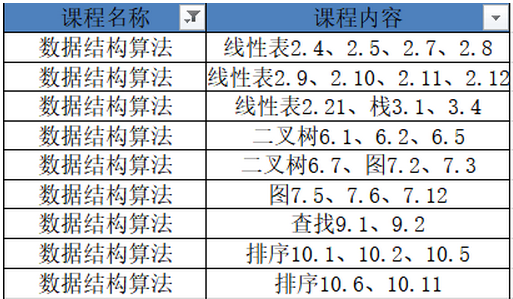
\includegraphics[scale=0.8]{example/chapter10/need.png}
\end{figure}

\section{算法实现}

\subsection{2.4}
\begin{lstlisting}[basicstyle=\small\ttfamily, caption={}, numbers=none]
算法思路:
顺序表在第i个元素之前插入一个元素时,需要移动第n个到第i个元素
\end{lstlisting}
\begin{lstlisting}[basicstyle=\small\ttfamily, caption={}, numbers=none]
Status ListInsert_Sq(SqList &L, int i, int e) {
	if (i < 1 || i>L.length + 1) return ERROR;
	if (L.length >= L.listsize) {
		newbase = (int *)realloc(L.elem, (L.listsize + LISTINCREMENT) * sizeof(int));
		if (!newbase) exit(OVErFLOW);
		L.elem = newbase;
		L.listsize += LISTINCREMENT;
	}
	q = &(L.elem[i - 1]);  // 第 i 个位置,因为从0开始的长度
	for (p = &(L.elem[L.length - 1]); p >= q; --p) { // p 指向最后一个元素,然后移动到后一个空元素
		*(p + 1) = *p;
	}
	*q = e;
	++L.length;
	return OK;
}
\end{lstlisting}

\subsection{2.5}
\begin{lstlisting}[basicstyle=\small\ttfamily, caption={}, numbers=none]
算法思路:
顺序表删除第i个元素,将第i+1至第n个元素一次向前移动一个位置
\end{lstlisting}
\begin{lstlisting}[basicstyle=\small\ttfamily, caption={}, numbers=none]
Status ListDelete_Sq(SqList &L, int i, int &e) {
	if (i < 1 || i>L.length + 1) return ERROR;
	q = &(L.elem[i - 1]);  // 第 i 个位置,因为从0开始的长度
	e = *q;
	p = L.elem + L.length - 1;
	for (q++; q <= p; ++q) { //
		*(q - 1) = *q;
	}
	--L.length;
	return OK;
}

\end{lstlisting}

\subsection{2.7}
\begin{lstlisting}[basicstyle=\small\ttfamily, caption={}, numbers=none]
算法思路:
合并两个顺序表,合并的两个顺序表也是有序的
\end{lstlisting}
\begin{lstlisting}[basicstyle=\small\ttfamily, caption={}, numbers=none]
void MergeList_Sq(SqList La, Sqlist Lb, SqList &Lc) {
	pa = La.elem; pb = Lb.elem;
	Lc.listsize = Lc.length = La.length + Lb.length;
	pc = Lc.elem = (int *)malloc(Lc.listsize * sizeof(int));
	if (!Lc.elem) exit(OVERFLOW);
	pa_last = La.elem + La.length - 1;
	pb_last = Lb.elem + Lb.length - 1;
	while (pb <= pa_last && pb <= pb_last) {
		if (*pa <= *pb) *pc++ = *pa++;
		else *pc++ = *pb++;
	}
	while (pa <= pa_last) *pc++ = *pa++;//插入a剩余元素
	while (pb <= pb_last) *pc++ = *pb++;//插入b剩余元素
}
\end{lstlisting}

\subsection{2.8}
\begin{lstlisting}[basicstyle=\small\ttfamily, caption={}, numbers=none]
算法思路:
链表得到元素
\end{lstlisting}
\begin{lstlisting}[basicstyle=\small\ttfamily, caption={}, numbers=none]
Status GetElem_L(LinkList L, int i, int & e) {
	p = L->next; j = 1;
	while (p && j<i)
	{
		p = p->next;
		++j;
	}
	if (!p || j > i)return ERROR;
	e = p->data;
	return OK;
}
\end{lstlisting}


\subsection{2.9}
\begin{lstlisting}[basicstyle=\small\ttfamily, caption={}, numbers=none]
算法思路:
链表插入元素
\end{lstlisting}
\begin{lstlisting}[basicstyle=\small\ttfamily, caption={}, numbers=none]
Status ListInsert_L(LinkList &L, int i, int e) {
	p = L;
	j = 0;
	while (p && j < i - 1) {
		p = p->next;
		++j;
	}
	if (!p || j < i - 1) return ERROR;
	s = (LinkList)malloc(sizeof(LNode));
	s->data = e;
	s->next = p->next;
	p->next = s;
	return OK;
}
\end{lstlisting}

\subsection{2.10}
\begin{lstlisting}[basicstyle=\small\ttfamily, caption={}, numbers=none]
算法思路:
链表删除元素
\end{lstlisting}
\begin{lstlisting}[basicstyle=\small\ttfamily, caption={}, numbers=none]
Status ListDelete_L(LinkList &L, int i, int &e) {
	p = L; j = 0;
	while (p->next && j < i - 1) {
		p = p->next; ++j;
	}
	if (!(p->next) || j > i - 1)
		return ERROR;
	q = p->next; p->next = q->next;
	e = q->data;
	free(q);
	return OK;
}
\end{lstlisting}

\subsection{2.11}
\begin{lstlisting}[basicstyle=\small\ttfamily, caption={}, numbers=none]
算法思路:
合并两个有序链表
\end{lstlisting}
\begin{lstlisting}[basicstyle=\small\ttfamily, caption={}, numbers=none]
void MergeList_L(LinkList &La, LinkList &Lb, LinkList &Lc) {
	pa = La->next; pb = Lb->next;
	Lc = pc = La;
	while (pa && pb) {
		if (pa->data <= pb->data) {
			pc->next = pa; pc = pa; pa = pa->next;
		}
		else {
			pc->next = pb; pc = pb; pb = pb->next;
		}
	}
	pc->next = pa ? pa : pb;
	free(Lb);
}
\end{lstlisting}


\subsection{2.12}
\begin{lstlisting}[basicstyle=\small\ttfamily, caption={}, numbers=none]
算法思路:
建立带头节点的单链线性表
\end{lstlisting}
\begin{lstlisting}[basicstyle=\small\ttfamily, caption={}, numbers=none]
void CreateList_L(LinkList &L, int n) {
	L = (LinkList)malloc(sizeof(LNode));
	L->next = NULL;
	for (int i = n; i > 0; --i) {
		p = (LinkList)malloc(sizeof(LNode));
		scanf(&p->data);
		p->next = L->next; L->next = p;
	}
}
\end{lstlisting}


\subsection{3.1}
\begin{lstlisting}[basicstyle=\small\ttfamily, caption={}, numbers=none]
算法思路:
利用栈实现非负十进制转为8进制
\end{lstlisting}
\begin{lstlisting}[basicstyle=\small\ttfamily, caption={}, numbers=none]
void conversion() {
	InitStack(S);
	scanf("%d", &N);
	while (N) {
		Push(S, N % 8);
		N = N / 8;
	}
	while (!StackEmpty(S)) {
		Pop(S, e);
		printf("%d", e);
	}
}
\end{lstlisting}


\subsection{3.4}
\begin{lstlisting}[basicstyle=\small\ttfamily, caption={}, numbers=none]
算法思路:
表达式求值
\end{lstlisting}
\begin{lstlisting}[basicstyle=\small\ttfamily, caption={}, numbers=none]
Status EvaluateExpression() {
	InitStack(OPTR); Push(OPRT, '#');//寄存运算符
	InitStack(OPND); c = getchar(); //OPND 寄存操作数或运算结果
	while (c != '#' || GetTop(OPTR) != '#') {
		if (!In(c, OP)) {
			Push(OPND, c);
			c = getchar();// 不是运算符,进栈
		}
		else {
			switch (Precede(GetTop(OPTR), c)) {
			case '<'://栈顶元素优先级低
					Push(OPTR, c); c = getchar();
					break;
			case '=':
				Pop(OPTR, x);
				c = getchar();
				break;
			case '>'://栈顶元素优先级低
				Pop(OPTR, theta);
				Pop(OPND, b);
				Pop(OPND, a);
				Push(OPND, Operate(a, theta, b));
				break;
			}
		}
	}
	return GetTop(OPND);
}
\end{lstlisting}

\subsection{6.1}
\begin{lstlisting}[basicstyle=\small\ttfamily, caption={}, numbers=none]
算法思路:
递归先序遍历
\end{lstlisting}
\begin{lstlisting}[basicstyle=\small\ttfamily, caption={}, numbers=none]
Status PreOrderTraverse(BiTree T, Status(*visit) (int e)) {
	if (T) {
		if (visit(T->data))
			if (PreOrderTraverse(T->lchild, visit))
				if (PreOrderTraverse(T->rchild, visit)) return OK;
		return ERROR;
	}
	else return OK;	
}
\end{lstlisting}


\subsection{6.2}
\begin{lstlisting}[basicstyle=\small\ttfamily, caption={}, numbers=none]
算法思路:
中序非递归算法
\end{lstlisting}
\begin{lstlisting}[basicstyle=\small\ttfamily, caption={}, numbers=none]
Status InOrderTraverse(BiTree T, Status(*Visit)(int e)) {
	InitStack(S);
	Push(S, T);//根指针进栈
	while (!StackEmpty(S)) {
		while (GetTop(S, &p) && p) Push(S, p->lchild); //向左走到尽头
		Pop(S, p); // 空指针退栈
		if (!StackEmpty(S)) {
			Pop(S, p);
			if (!Visit(p->data))
				return ERROR;
			Push(S, p->rchild);// 访问节点向右一步
		}
	}
	return OK;
}
\end{lstlisting}

\subsection{6.5}
\begin{lstlisting}[basicstyle=\small\ttfamily, caption={}, numbers=none]
算法思路:
中序线索化二叉树的遍历
\end{lstlisting}
\begin{figure}[H]
	\centering  % 环境中的内容居中排版
	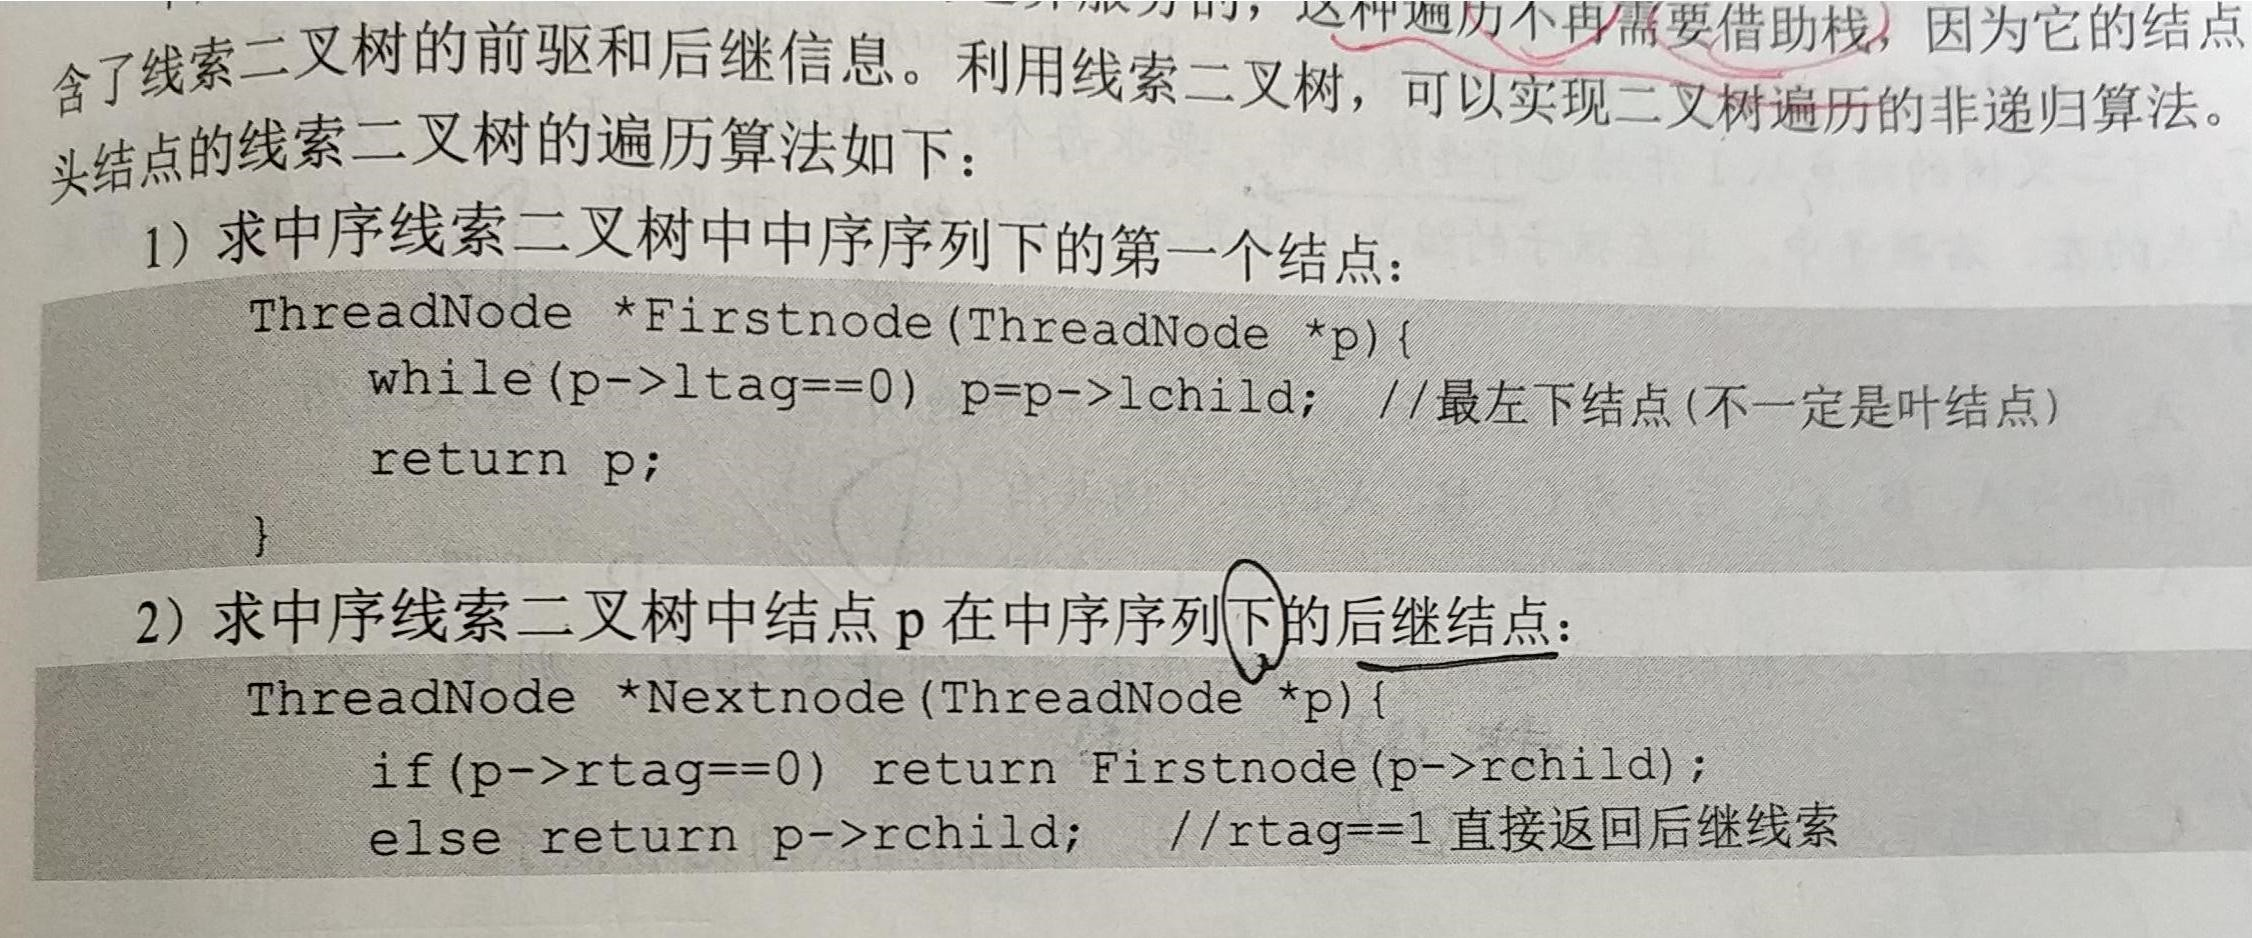
\includegraphics[scale=0.3]{example/chapter10/Img_181217111812632-1.jpg}
\end{figure}

\subsection{6.7}
\begin{lstlisting}[basicstyle=\small\ttfamily, caption={}, numbers=none]
算法思路:
中序线索化  不带头结点
\end{lstlisting}
\begin{figure}[H]
	\centering  % 环境中的内容居中排版
	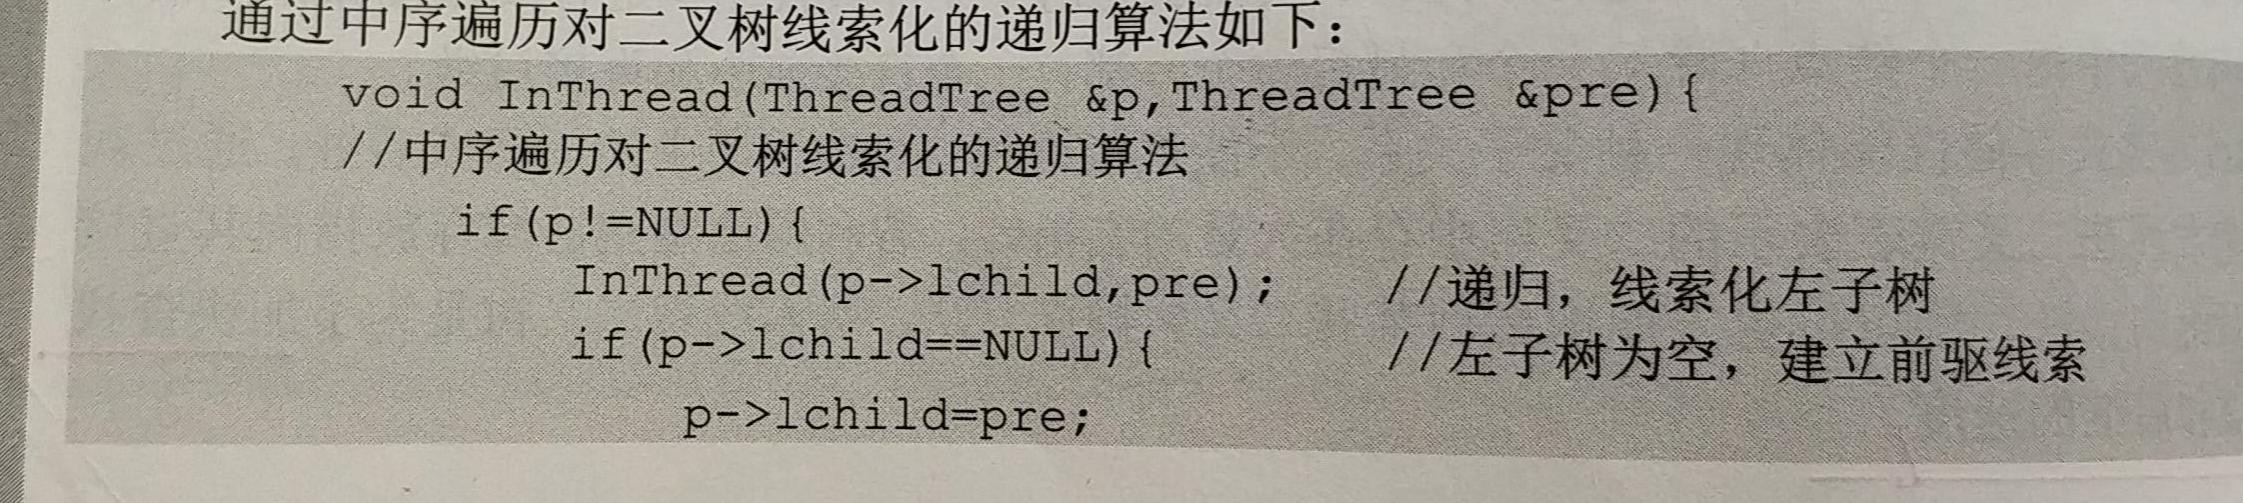
\includegraphics[scale=0.3]{example/chapter10/Img_181217112900037-1.jpg}
\end{figure}
\begin{figure}[H]
	\centering  % 环境中的内容居中排版
	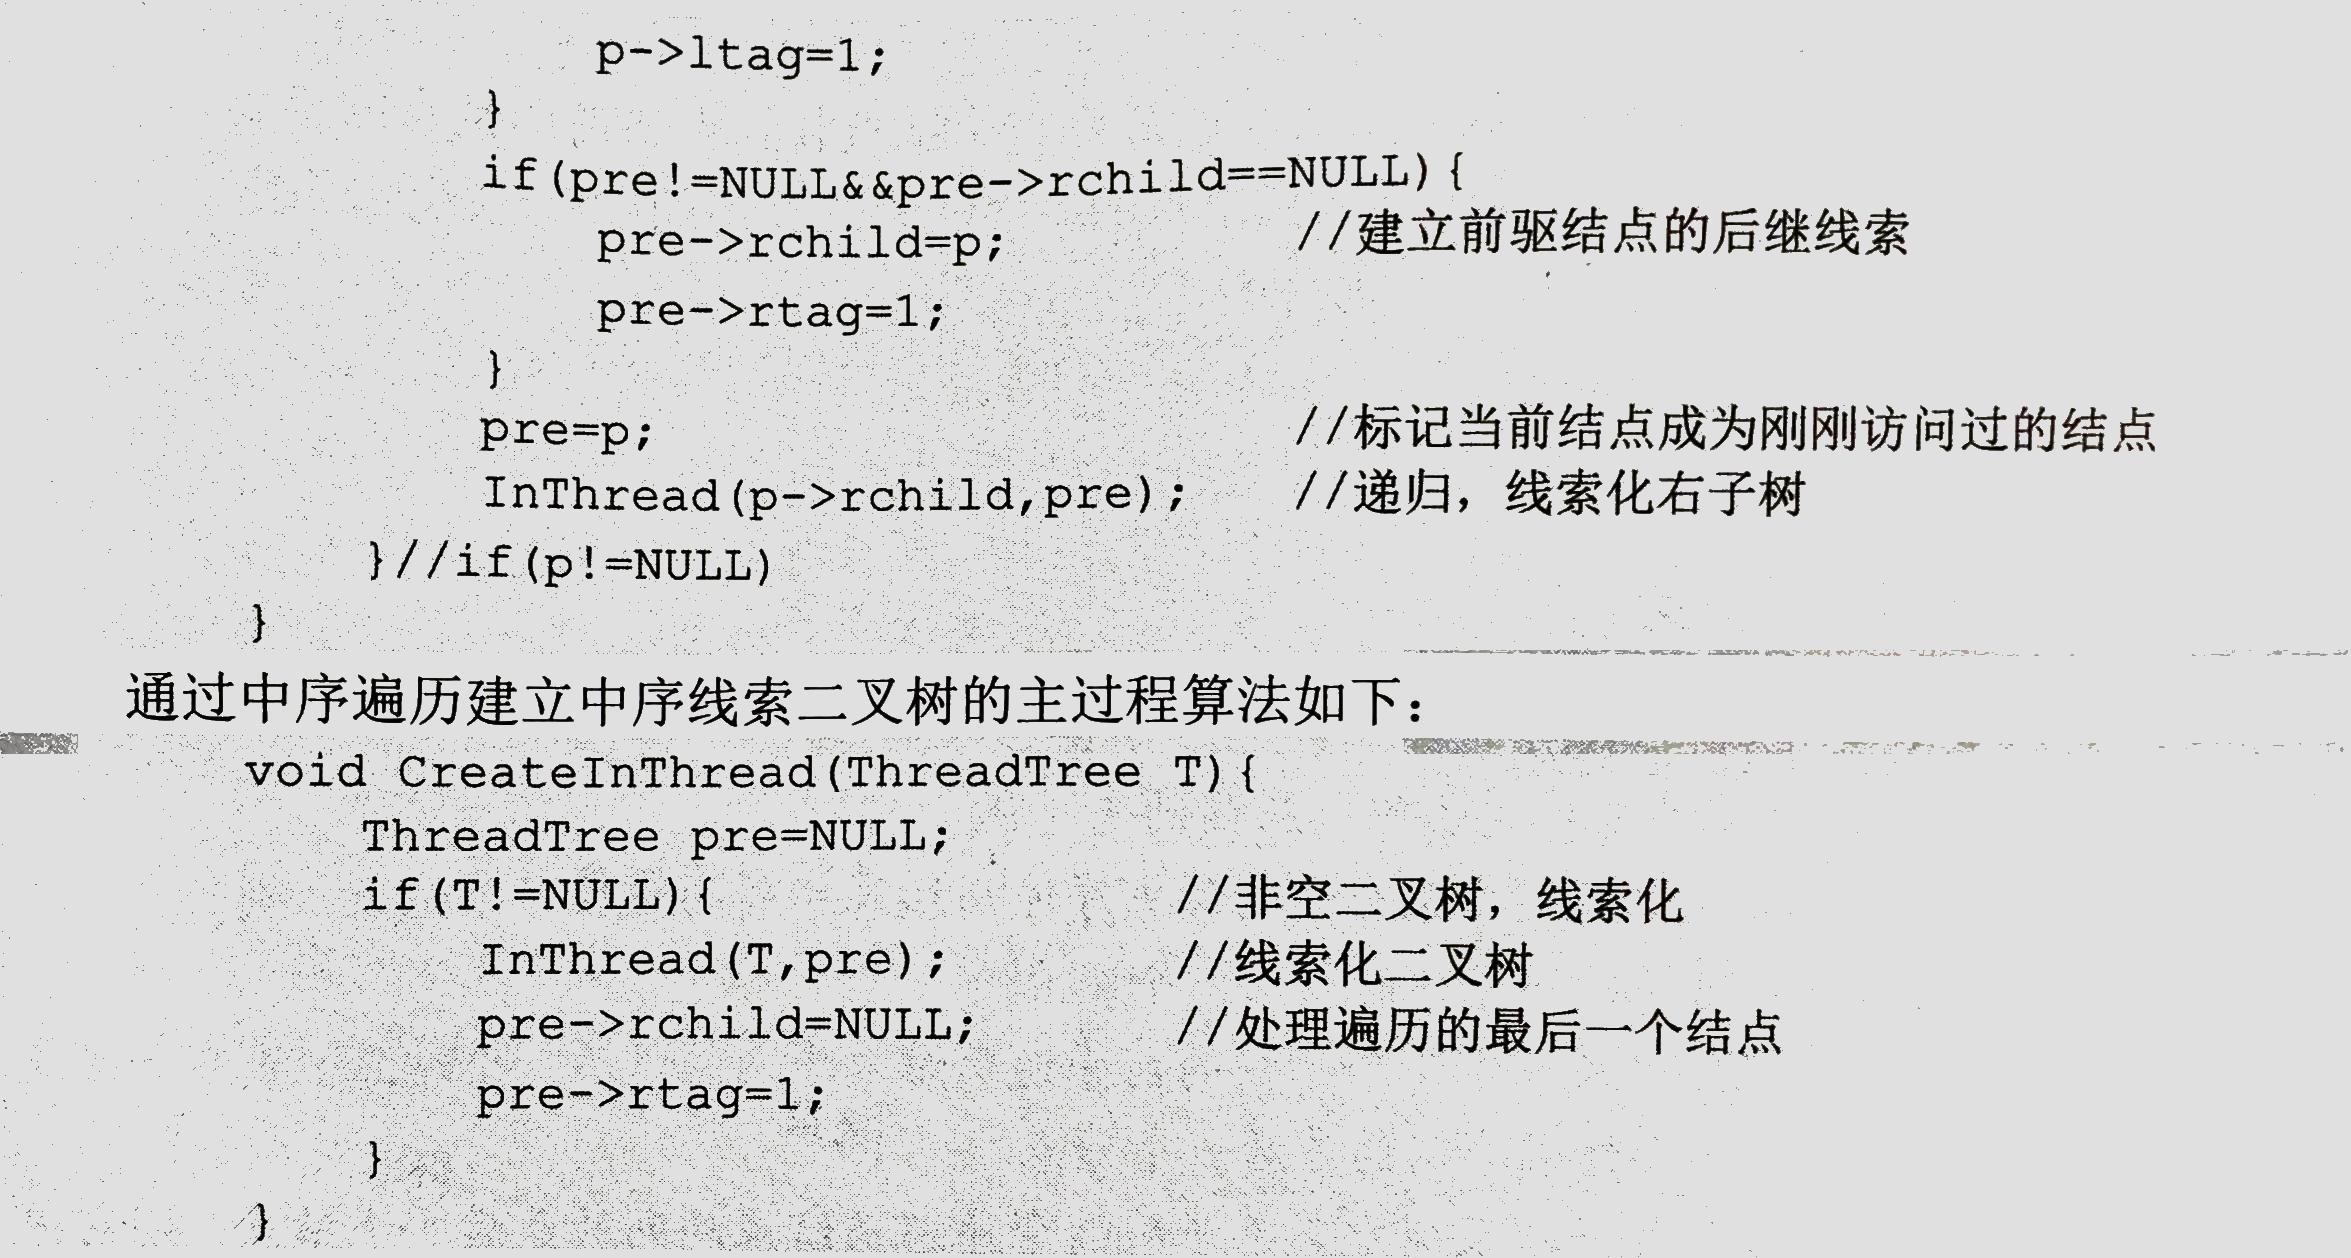
\includegraphics[scale=0.3]{example/chapter10/Img_181217112940976-1.jpg}
\end{figure}

\subsection{7.2}
\begin{lstlisting}[basicstyle=\small\ttfamily, caption={}, numbers=none]
算法思路:
构造无向网
\end{lstlisting}
\begin{lstlisting}[basicstyle=\small\ttfamily, caption={}, numbers=none]
Status CreateUND(MGraph &G) {
	//构造无向图
	scanf(&G.vexnum, &G.arcnum, &IncInfo);
	for (int i = 0; i < G.vexnum; ++i) {
		scanf(&G.vexs[i]);// 构造顶点向量
	}
	for (i = 0; i < G.vexnum; ++i) {// 初始化邻接矩阵
		for (j = 0; j < G.vexnum; ++j) {
			G.arcs[i][j] = { INFINITY, NULL };
		}
	}
	for (k = 0; k < G.vexnum; k++) {
		scanf(&v1, &v2, &w);
		i = LocateVex(G, v1); j = LocateVex(G, v2); // 确定v1和v2在G中的位置
		G.arcs[i][j].adj = w; // 弧的全职
		if (IncInfo) Input(*G.arcs[i][j].info);// 若弧含有相关信息则输入
		G.arcs[j][i] = G.arcs[i][j];
	}
	return OK;
}
\end{lstlisting}


\subsection{7.2}
\begin{lstlisting}[basicstyle=\small\ttfamily, caption={}, numbers=none]
算法思路:
采用十字链表存储表示,构造有向图G
\end{lstlisting}
\begin{lstlisting}[basicstyle=\small\ttfamily, caption={}, numbers=none]
			Status CreateDG(OLGraph &G) {
				scanf(&Gvexnum, &G.arcnum, &IncInfo);
				for (int i = 0; i < G.vexnum; ++i) {
					scanf(&G.xlist[i].data);// 输入顶点值
					G.xlist[i].firstin = NULL; G.xlist[i].firstout = NULL;
				}
				for (k = 0; k < G.arcnum; k++) {
					scanf(&v1, &v2);// 输入一条弧的起点和终点
					i = LocateVex(G, v1); j = LocateVex(G, v2);
					p = (ArcBox *)malloc(sizeof(ArcBox));
					*p = { i,j,G.xlist[j].firstin, G.xlist[i].firstout,NULL };
					//{tailvex, headvex, hlink, tlink, info}
					G.xlist[j].firstin = G.xlist[i].firstout = p;// 完成在入弧和出弧链头的插入
					if (IncInfo)Input(*p->info);
				}
			}

\end{lstlisting}


\subsection{7.5}
\begin{lstlisting}[basicstyle=\small\ttfamily, caption={}, numbers=none]
算法思路:
DFS
\end{lstlisting}
\begin{lstlisting}[basicstyle=\small\ttfamily, caption={}, numbers=none]
void DFS(Graph G, int v) {
	visited[v] = true;
	VisitFunc(v);
	for (w = FirstAdjVex(G, v); w >= 0; w = nextAdjVex(G, v, w)) {
		if (!visited[w])
			DFS(G, w);
	}
}
\end{lstlisting}


\subsection{7.6}
\begin{lstlisting}[basicstyle=\small\ttfamily, caption={}, numbers=none]
算法思路:
BFS
\end{lstlisting}
\begin{lstlisting}[basicstyle=\small\ttfamily, caption={}, numbers=none]
void BFSTraverse(Graph G, Status(*Visit)(int v)) {
	for (v = 0; v < G.vexnum; ++v) {
		visited[v] = FALSE;
	}
	InitQueue(Q);
	//初始化
	for (v = 0; v < G.vexnum; ++v) {
		if (!visited[v]) {
			visited[v] = true;
			Visit(v);
			EnQueue(Q, v);
			while (!QueueEmpty(Q)) {
				DeQueue(Q, u); // 对头元素出对,并置为u;
				for (w = FirstAdjVex(G, u); w >= 0; w = NextAdjVex(G, u, w)) {//w 为 u尚未访问的邻接顶点
					if (!Visit[w]) {
						Visited[w] = true;
						Visit(w);
						EnQueue(Q, W);
					}
				}
			}
		}
	}
}

\end{lstlisting}

\subsection{7.12}
\begin{lstlisting}[basicstyle=\small\ttfamily, caption={}, numbers=none]
算法思路:
拓扑排序
\end{lstlisting}
\begin{lstlisting}[basicstyle=\small\ttfamily, caption={}, numbers=none]
Status TopologicalSort(ALGraph G) {
	// 有向图采用邻接表存储结构
	// 若G 无回路,则输出G的顶点的一个拓扑序列并返回OK,否则ERROR
	FindInDegree(G, indegree);// 对各顶点求入读 indegree[0..vernum-1];
	InitStack(S);
	for (i = 0; i < G.vexnum; ++i) {
		if (!indegree[i]) Push(S, i);// 如果入度为0进栈
	}
	count = 0;
	while (!StackEmpty(S)) {
		Pop(S, i);
		printf(i, G.vertices[i].data); // 输出i号顶点并计数
		++count;
		for (p = G.vertices[i].firstarc; p; p = p->nextarc) {
			k = p->adjvex; // 对i 号顶点的每个邻接点的入读减1
			if (!(--indegree[k]))
				Push(S, k);// 若入度为0则入栈
		}
	}
	if (count < G.vexnum) return ERROR;// 该有向图有回路
	else
		return OK;
}

\end{lstlisting}

\subsection{9.1}
\begin{lstlisting}[basicstyle=\small\ttfamily, caption={}, numbers=none]
算法思路:
在数组里面查找某个元素
\end{lstlisting}
\begin{lstlisting}[basicstyle=\small\ttfamily, caption={}, numbers=none]
int Serach_Seq(SSTable ST, KeyType key) {
	// 在顺序表ST中顺序查找其关键字等于key的数据元素,若找到,则函数值为
	// 该元素在表中的位置,否则为0
	ST.elem[0].key = key;
	for (i = ST.length; !EQ(ST.elem[i].key, key); --i);
	return i;
}
\end{lstlisting}

\subsection{9.1}
\begin{lstlisting}[basicstyle=\small\ttfamily, caption={}, numbers=none]
算法思路:
折半查找
\end{lstlisting}
\begin{lstlisting}[basicstyle=\small\ttfamily, caption={}, numbers=none]
int Search_Bin(SSTable ST, KeyType key) {
	// 在有序表ST中折半查找其关键字等于key的数据元素。若找到,则函数值为
	// 该元素在表中的位置,否则为0
	low = l; high = ST.length;
	while (low <= high) {
		mid = (low + high) / 2;
		if (EQ(key, ST.elem[mid].key)) return mid;
		else if (LT(key, ST.elem[mid].key)) high = mid - 1;
		else
			low = mid + 1;
	}
	return 0;
}
\end{lstlisting}

\subsection{10.1}
\begin{lstlisting}[basicstyle=\small\ttfamily, caption={}, numbers=none]
算法思路:
直接插入排序
\end{lstlisting}
\begin{lstlisting}[basicstyle=\small\ttfamily, caption={}, numbers=none]
void InsertSort(SqList &L) {
	// 对顺序表L作直接插入排序
	for (i = 2; i <= L.length; ++i) {
		if (LT(L.r[i].key, L.r[i - 1].key)) {
			L.r[0] = L.r[i]; // 哨兵
			L.r[i] = L.r[i - 1];
			for (j = i - 2; LT(L.r[0], L.r[j].key); --j) {
				L.r[j + 1] = L.r[j]; // 记录后移
			}
			L.r[j + 1] = L.r[0];//插入到正确位置
		}
	}
}
\end{lstlisting}

\subsection{10.2}
\begin{lstlisting}[basicstyle=\small\ttfamily, caption={}, numbers=none]
算法思路:
折半插入排序
\end{lstlisting}
\begin{lstlisting}[basicstyle=\small\ttfamily, caption={}, numbers=none]
void BInsrtSort(SqList &L) {
	for (i = 2; i <= L.length; i++) {
		L.r[0] = L.r[i];
		low = 1; high = i - 1;
		while (low <= high) {
			m = (low + high) / 2;
			if (LT(L.r[0].key, L.r[m].key)) high = m - 1;
			else low = m + 1;
		}
		for (j = i - 1; j >= high + 1; --j) {
			L.r[j + 1] = L.r[j];//记录后移
		}
		L.r[hgih + 1] = L.r[0];
	}
}
\end{lstlisting}


\subsection{10.5}
\begin{lstlisting}[basicstyle=\small\ttfamily, caption={}, numbers=none]
算法思路:
希尔排序
\end{lstlisting}
\begin{lstlisting}[basicstyle=\small\ttfamily, caption={}, numbers=none]
void ShellInsert(SqList &L, int dk) {
	// 对顺序表L做一趟希尔排序。本算法时和一趟直接插入排序相比做了以下修改
	// 1.前后记录位置的增量时dk,而不是1
	// 2.r[0]只是暂存单元不是哨兵。当j<=0时,插入位置已找到。
	for (i = dk + 1; i <= L.length; i++) {
		if (LT(L.r[i].key, L.r[i - dk].key)) {
			L.r[0] = L.r[i];
			for (j = i - dk; j > -&&LT(L.r[0].key, L.r[j].key); j -= dk) {
				L.r[j + dk] = L.r[j];
			}
			L.r[j + dk] = L.r[0];
		}
	}
}
void ShellShort(SqList &L, int dlta[], int t) {
	for (k = 0; k < t; ++k) {
		ShellInsert(L, dlta[k]);
	}
}
\end{lstlisting}


\subsection{10.6}
\begin{lstlisting}[basicstyle=\small\ttfamily, caption={}, numbers=none]
算法思路:
快速排序
\end{lstlisting}
\begin{lstlisting}[basicstyle=\small\ttfamily, caption={}, numbers=none]
int Partition(SqList &L, int low, int high) {
	// 交换顺序表L中字表L.r[low...high]的记录,使枢轴记录到位,并返回其所在位置,此时
	// 在它之前(后)的记录均不大(小)于它。
	pivotkey = L.r[low].key;// 用子表的第一个记录做枢轴量技术
	while (low < high) {
		while (low < high && L.r[high].key >= pivotkey) --high;
		swap(L.r[low], L.[high]);
		while (low < high && L.r[low].key <= pivotkey) ++low;
		swap(L.r[low], L.r[high]);
	}
	return low;
}
void QSort(SqList &L, int low, int high) {
	if (low < high) {
		povotloc = Partition(L, low, high);
		Qsort(L, low, pivotloc - 1);
		QSort(L, pivotloc + 1, high);
	}
}
\end{lstlisting}


\subsection{10.6}
\begin{lstlisting}[basicstyle=\small\ttfamily, caption={}, numbers=none]
算法思路:
堆排序
\end{lstlisting}
\begin{lstlisting}[basicstyle=\small\ttfamily, caption={}, numbers=none]
void AdjustDown(int A[],int k, int len) {
	A[0] = A[k];
	for (i = 2 * k; i <= len; i*=2) {
		if (i < len&&A[i] < A[i + 1]) {
			i++;
		}
		if (A[0] >= A[i]) break;
		else {
			A[k] = A[i];
			k = i;
		}
	}
	A[k] = A[0];
}

void BuildMaxHeap(int A[], int n) {
	for (int i = n / 2; i > 0; i--) {
		AdjustDown(A, len, i);
	}
}
void HeapSort() {
	BuildMaxHeap(A, len);
	for (i = len; i > 1; i--) {
		swap(A[i], A[1]);
		AdjustDown(A, 1, i - 1);
	}
}
\end{lstlisting}






 % 算法背诵
%\chapter{时间复杂度的计算}
\label{chap11}
\begin{itemize}[noitemsep,topsep=0pt,parsep=0pt,partopsep=0pt]
	\item 知识点:讲解相关知识点。
	\item 题型:直接上真题。
\end{itemize}

\section{知识点和方法论}

\subsection{知识点}
\begin{itemize}[noitemsep,topsep=0pt,parsep=0pt,partopsep=0pt]
	\item 时间复杂度常用大 O 符号表示
	\item 时间复杂度是去掉最高项多项式前面的系数,且不包括函数的低阶项。
	\item 常见时间复杂度$Ο(1)<Ο(log_2 n)<Ο(n)<Ο(nlog_2 n)<Ο(n^2)<Ο(n^3)<Ο(2^n)<O(n!)<O(n^n)$
	\item 空间复杂度如果,算法原地工作那么,空间复杂度为O(1)
\end{itemize}

\subsection{方法论}
\begin{itemize}[noitemsep,topsep=0pt,parsep=0pt,partopsep=0pt]
	\item 简单计算相关的要计算的函数关键语句执行的次数。
	\item 对于关键语句使用令 关键语句执行的次数是 t 次。
\end{itemize}

\section{真题实战}

\subsection{2011年408}
设n是描述问题规模的非负整数,下面程序片段的时间复杂度是( )
\begin{lstlisting}[basicstyle=\small\ttfamily, caption={}, numbers=none]
x = 2;
while(x < n/2)
	x=2*x; // 3
\end{lstlisting}
解:\newline
{\color{red}(计算函数关键语句的执行次数)}\newline
令: 第三行语句执行了t次,\newline
可知条件不满足的情况是$ x*2^t >= n/2 $,其中x = 2\newline
所以条件不满足的情况 $ 2^{t+1} >= n/2  $ \newline
求解t: 可知 $t >= log_2(n) - 2$ \newline
舍去低阶项,可知 $ t >= log_2(n)$ \newline
再用大O表示,可得时间复杂度为 $O(log_2 n)$

\subsection{2014年408}
下面程序片段的时间复杂度是( )
\begin{lstlisting}[basicstyle=\small\ttfamily, caption={}, numbers=none]
count=0;
for(k=1; k<=n; k*=2)// 1
	for(j=1; j<=n; j++) // 2
		count++;// 3
\end{lstlisting}
解:\newline
{\color{red}(计算函数关键语句的执行次数)}\newline
计算 3 语句的频度\newline
已知:for里面for循环导致3语句执行次数是两个for次数相乘\newline
令 1语句中 k*=2 执行了 t 次。
1 语句可以执行 $ k*2^t > n $ \newline
可得 $ t > log_2 (n) $ \newline
1的每个循环中,易知 2 语句中 j++ 执行了 n 次。\newline
易知,3语句的执行次数和2语句中 j++是一样的的。\newline
得到总执行次数$ log_2 (n) * n$ (前面的系数忽略)\newline
易知,时间复杂度为 $ log_2 (n) * n $\newline

\subsection{2017年408}
下列函数的时间复杂度是( )
\begin{lstlisting}[basicstyle=\small\ttfamily, caption={}, numbers=none]
int func(int n){
	int i=0; sum=0;
	while(sum < n) 
		sum += ++i;\\ 4
	return i;
}
\end{lstlisting}
解:\newline
{\color{red}(计算函数关键语句的执行次数)}\newline
可知i的变化是 1,2,3,4,5...\newline
令 4 语句执行了 t 次\newline
sum = 1 + 2 + 3 + ... + t \newline
可知当条件不满足时$ sum = \frac{t * (1 + t)}{2} >= n $\newline
得知 $ t + t^2 >= 2n$\newline
忽略低次项$ t >= \sqrt{2*n} $\newline
忽略常数项的系数 $ t >= \sqrt{n}$ \newline
得知时间复杂度是 $ O(\sqrt{n})$






 % 时间复杂地计算
%\chapter{线性表队列栈的计算}
\label{chap12}
\begin{itemize}[noitemsep,topsep=0pt,parsep=0pt,partopsep=0pt]
	\item 知识点:讲解相关知识点。
	\item 题型:直接上真题。
\end{itemize}

\section{知识点和方法论}

\subsection{知识点}
\begin{itemize}[noitemsep,topsep=0pt,parsep=0pt,partopsep=0pt]
	\item 线性表中的位子序列从{\color{red}1}开始,计算机中的数组从{\color{red}0}开始。
	\item 卡特兰数:n个不同元素入栈,出栈序列的个数为 $\frac{1}{n+1} C^{n}_{2n} = \frac{1}{n+1}\frac{(2n)!}{n! \times n!} $
	\item 后缀表达式也成为,逆波兰式。
	\item 在考试中简单的栈实现和队列实现
	\begin{itemize}[noitemsep,topsep=0pt,parsep=0pt,partopsep=0pt]
		\item 申明一个栈并初始化 int stack[maxSize]; int top=-1;
		\item 元素入栈 stack[++top] = x;
		\item 元素出栈 x= stack[top--];
	\end{itemize}
\end{itemize}

\subsection{方法论}
\begin{itemize}[noitemsep,topsep=0pt,parsep=0pt,partopsep=0pt]
	\item 如何想不出来只遍历一遍的方法,使用普通方法也可得到大部分的分数。
	\item 中缀表达式转为后缀表达式:\newline
		1. 栈中只存放符号\newline
		2. 处理括号\newline
			i. 若为 '(' 存入栈中。\newline
			ii. 若为 ')' 将 '(' 之前的符号依次弹出\newline
		3. 运用四则运算法则,比如\newline
			i.  栈顶'+' 小于扫描到的 '/' , '/' 入栈\newline
			ii. 栈顶'/' 大于扫描到的 '+' , '/' 出栈, '+' 入栈\newline
		4. 检验从后往前依次读取计算,看是否和预料到的相同。\newline
\end{itemize}

\section{真题实战}

\subsection{王道2019年线性表第10题}
若长度为n的非空线性表采用顺序存储结构,在表的第i个位置插入一个数据元素,i的合法值应该是(   )
解:\newline
线性表中的位子序列从{\color{red}1}开始,计算机中的数组从{\color{red}0}开始\newline
隐含条件是原先第i个位子如果有元素,其和其后的元素后移。易知是  $ 1 \le i \le n+1 $

\subsection{2010年408}
设将n(n>1)个整数存放到一维数组R中。试设计一个在时间和空间两方面都尽可能高效的算法。
将R中保存的序列循环左移p(0<p<n)个位置,即将R中的数据由(X0,X1,X2...Xn-1)变换为(Xp,Xp+1...Xn-1,X0,X1,...,Xp-1).要求:\newline
1. 给出算法的基本设计思想.\newline
2. 根据设计思想,采用C或C++语言描述算法,关键之处给出注释。\newline
3. 说明你所设计算法的时间复杂度和空间复杂度. \newline
解:(可能一开始想不出特别好的方法或者当你速度特别慢的时候,记得先把一种最容易的方法写上去,如果是正确的但是时间和空间复杂度不是最优秀的也可以得到10/15分的成绩)\newline
1) 算法设计思想:\newline
1. 先把数组 0 - (p-1) 个反转\newline
2. 再把数组 p - 最后 反转\newline
3. 最后吧整个数组反转\newline
2)\newline
\begin{lstlisting}[basicstyle=\small\ttfamily, caption={}, numbers=none]
#include <iostream>
#include <algorithm>
using namespace std;
// reverse(first, last)
// (1) first表示要排序数组的起始地址;
// (2) last表示数组结束地址的下一位;
// A 数组  p 左移个数  len 数组长度
void shiftLeft(int A[], int p, int len) { // 写出这个函数带上头文件 algorithm 就可以算对了
	reverse(A, A + p);
	reverse(A + p, A + len);
	reverse(A, A + len);
}

int main() {
	int a[] = { 1, 2, 3, 4, 5, 6, 7, 8, 9 };
	shiftLeft(a, 4, 9);
	for (int i = 0; i < 9; i++) {
		cout << a[i] << " ";
	}
	cout << endl;
	system("pause");
}
\end{lstlisting}
3)\newline
时间复杂度\newline
整个序列反转一次,相当于对一半的元素执行了交换,( temp = a; a = b; b =temp;) 执行次数为 n / 2 * 3.总共相当于两次执行整个序列的反转。执行次数是n * 3,时间复杂度易知是 O(n) , 空间复杂度,因为没有额外增加其他的空间,算法原地工作,所以是 O(1).\newline

---------\newline

另解:\newline
1) 算法设计思想:\newline
1. 先把数组 0 - (p-1) 个存放在一个额外的数组中,再原数组向左平移p个单位,最后吧额外数组中的元素复制到后面\newline
2)\newline
\begin{lstlisting}[basicstyle=\small\ttfamily, caption={}, numbers=none]
#include <iostream>
#include <algorithm>
#include <vector>
using namespace std;
// reverse(first, last)
//(1)first表示要排序数组的起始地址;
//(2)last表示数组结束地址的下一位;
// A 数组  p 左移个数  len 数组长度
void shiftLeft1(int A[], int p, int len) {
	reverse(A, A + p);
	reverse(A + p, A + len);
	reverse(A, A + len);
}

void shiftLeft2(int A[], int p, int len) {
	vector<int> v;
	for (int i = 0; i < p; i++) {
		int tmp = A[i];
		v.push_back(tmp);
	}
	for (int i = p,j = 0; i < len; i++, j++) {
		A[j] = A[i];
	}
	for (int i = len - p,j =0; i < len; i++,j++) {
		A[i] = v[j];
	}
}


int main() {
	int a[] = { 1, 2, 3, 4, 5, 6, 7, 8, 9 };
	shiftLeft2(a, 4, 9);
	for (int i = 0; i < 9; i++) {
		cout << a[i] << " ";
	}
	cout << endl;
	system("pause");
}
\end{lstlisting}
3)\newline
时间复杂度\newline
前p个元素复制了两次2*p,后n - p 个元素转移了一次 ,总共 n + p 次,时间复杂度是 O(n)\newline
空间复杂度,增加了p个空间,所以是 O(p) .\newline

\subsection{2009年线性表408}
已知一个带有表头节点的单链表,节点结构为 data, link (杭电考试一般会给出结构体)\newline
假设该链表只给出了头指针list。在不改变链表的前提下,请设计一个尽可能高效的算法,查找链表中倒数第K个位置上的节点(K为正整数)。若查找成功,算法出书该节点的data域的值,并返回1;否则只返回0.\newline
1. 给出算法的基本设计思想.\newline
2. 描述算法的纤细时间步骤.\newline
3. 根据设计思想,采用C或C++语言描述算法,关键之处给出注释。\newline

解:\newline
1)\newline
算法的基本设计思想是:(王道上面写的很详细,照搬了)\newline
关键一遍遍历,设定两个指针,一个指针只管往下遍历,另一个指针,在第一个指针,开始遍历次数统计为k的时候开始遍历。第二个指针如果运动了的话,那么就证明倒数第k个节点存在。\newline
2)\newline
1. 初始化: count = 0, p 和 q 指针指向第一个节点。\newline
2. 开始遍历: p 只要没有遇到 NULL 节点就一直往下遍历,同时count开始计数,当count >= k时q才开始遍历。
3. 判断: 如果count < k时, 说明没有倒数第 k 个节点,返回0结束。否则输出第k个节点的值,然后 返回 1.
3)\newline
\begin{lstlisting}[basicstyle=\small\ttfamily, caption={}, numbers=none]
#include <iostream>
using namespace std;

typedef struct LNode {// 关键处的注释 略
	int data;
	struct LNode *link;
}LNode;

int search_k(LNode* list, int k) {
	LNode *p = list->link, *q = list->link;
	int count = 0;
	while (p != NULL) {
		if (count < k) count++;
		else q = q->link;
		p = p->link;
	}
	if (count < k)
	return 0;
	else {
		printf("%d", q->data);
		return 1;
	}
}

int main() {
	//创建节点
	
	//创建头结点
	LNode *list = (LNode *)malloc(sizeof(LNode));
	list->data = -1;
	list->link = NULL;
	LNode *q = list;
	for (int i = 0; i < 10; i++) {
		LNode *p = (LNode *)malloc(sizeof(LNode));
		p->data = i;
		p->link = NULL;
		q->link = p;
		q = p;
	}
	q = list;
	while (q) {
		cout << q->data << endl;
		q = q->link;
	}
	system("pause");
}
\end{lstlisting}
-------\newline
其他想法:\newline
把遍历的结果存放入一个额外数组中,然后,直接判断 len - k 是否小于 0, 但是结果只能得到 10分。\newline


\subsection{2012年线性表408}
假定采用带头结点的单链表保存单词,当两个单词有相同的后缀是,则可共享相同的后缀存储空间,例如,"loading" 和 "being"的存储映像如下所示。\newline
设str1 和str2 分别指向两个单词所在单链表的头结点,链表的节点结构为[data, next],请设计一个时间上尽可能高效的算法,找出由str1和str2所指向两个链表共同后缀的起始位置。\newline
1. 给出算法的基本设计思想.\newline
2. 根据设计思想,采用C或C++语言描述算法,关键之处给出注释。\newline
3. 说明你所设计算法的时间复杂度. \newline

解:\newline
1)\newline
算法的基本设计思想是:(王道上面写的很详细,照搬了)\newline
1. 计算两个单词的长度。\newline
2. 将 p 和 q 分别指向两个单词,同时将长的单词的指针,和短的指针长度对齐,然后开始遍历直到他们找到共同的节点。\newline
2)\newline
\begin{lstlisting}[basicstyle=\small\ttfamily, caption={}, numbers=none]
typedef struct LNode {
	char data;
	struct LNode *next;
}LNode;
/*求链表长度*/
int listlen(LNode* head) {
	int len = 0;
	while (head->next != NULL) {
		len++;
		head = head->next;
	}
	return len;
}
/* 找出统统后缀的起始地址 */
LNode * find_addr(LNode *str1, LNode *str2) {
	int m, n;
	LNode *q, *p;
	m = listlen(str1); // p 对应 m
	n = listlen(str2); // q 对应 n
	for (p = str1; m > n; m--)
		p = p->next;
	for (q = str2; m < n; n--)
		q = q->next;
	//现在p和q在倒数相同的位置上,确定他们的共同位置
	while (p->next != NULL && p->next != q->next) {
		p = p->next;
		q = q->next;
	}
	return q->next;
}
\end{lstlisting}
3)\newline
时间复杂度:\newline
{\color{red}一般指最坏时间复杂度} 由此得知, 计算两个长度为  m+n, 对齐假设啥都不干, 只有最后一个字符是他们共同的节点,那么就可以得出右遍历了一次, 最大时间复杂度是 $ 2 \times (m + n) $, 所以时间复杂度是 O(m + n). 空间复杂度是O(1), 原地操作

\subsection{王道有意义的题}
3个不同元素一次进栈,能得到( ) 不同的出栈序列。\newline

解:\newline
使用卡特兰数公式:$\frac{1}{3+1}\frac{(6)!}{3! \times 3!} = 5$ 种不同的出栈序列。

\subsection{2014年计算机408}
假设栈初始为空,将中缀表达式a/b+(c*d - e*f)/g 转换为等价的后缀表达式的过程中,当扫描到f时,栈中的元素依次是( ).\newline
解:\newline
栈: push(/),'/' > '+' pop('/') push('+'),push'(', push'*','*' > '-' push '-' pop '*','-' < '*'  push '*', == +,'(',-,'*'\newline
打印序列: a,b,'/',c,d,'*',e,f \newline
继续\newline
栈:pop'*' pop'-' del'(', '+' < '/' push '/',pop '/', pop '+'\newline
打印序列: '*''-',g,'/''+'\newline





 % 线性表队列栈
%%# -*- coding: utf-8-unix -*-
%%==================================================

\chapter{查找与排序}
\label{chap13}

\begin{itemize}[noitemsep,topsep=0pt,parsep=0pt,partopsep=0pt]
	\item 知识点:讲解相关知识点。
	\item 题型:直接上真题。
\end{itemize}

\section{知识点和方法论}

\subsection{知识点}
\begin{itemize}[noitemsep,topsep=0pt,parsep=0pt,partopsep=0pt]
	\item 查找成功长度和查找失败长度
	\item 折半查找算法
	\item 折半查找树的绘制
	\item 各种排序知道整体的流程
	\item 快速排序的partation代码要记住,可能要考试。
\end{itemize}

\subsection{方法论}

\section{真题实战}

\subsection{2010年408}
已知一个长度为16的顺序表L,七元素按关键字有序排列,若采用折半查找发查找一个L中不存储在的元素,则关键字的比较次数最多是(  )\newline
解:\newline
折半查找失败最多次数是树的高度求树的高度得到$\left \lfloor log_2{n} \right \rfloor + 1$ 就可以得到树的高度。\newline


\subsection{王道简单题}
具有12个关键字的有序表中,对每个关键字的查找概率相同,折半查找查找成功的平均查找长度为(   ), 者半查找查找失败的平均查找长度为(  ).\newline
A. 37/12   B. 35/12 C. 39/13 D. 49/13 \newline
解:\newline
记住折半查找算法的开始位置是从0开始到len-1结束。一定要画出者半查找树\newline
算查找失败的次数只要算下面方括号的上面的结点的wpl,再处于元素的个数\newline
\begin{figure}[H]
	\centering  % 环境中的内容居中排版
	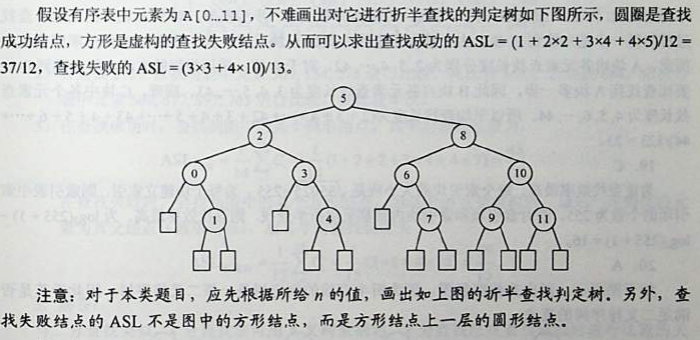
\includegraphics[scale=1]{example/chapter13/Annotation2019-09-25181550.png}
\end{figure}

\subsection{王道简单题考察希尔排序}
若数据元素序列{98, 36, -9, 0, 47,23, 1, 8, 10, 7}采用希尔排序系列序列是增量为4的一趟排序结果。\newline
解:\newline
\begin{figure}[H]
	\centering  % 环境中的内容居中排版
	\includegraphics[scale=0.1]{example/chapter13/IMG_20190925_191655.jpg}
\end{figure}

\subsection{2015年408}
希尔排序的组内排序是()\newline
解:\newline
易知是直接插入排序。\newline

\subsection{2009年408}
若数据元素序列{11,12,13,7,8,9,23,4,5}是采用系列排序方法之一得到的第二趟排序后的结果,则该排序算法只能是(   )\newline
插入排序,因为局部有序,冒泡和选择都是有一些位置在他们最终的位置上。\newline













 % 查找与排序
%%# -*- coding: utf-8-unix -*-
%%==================================================

\chapter{查找与排序}
\label{chap13}

\begin{itemize}[noitemsep,topsep=0pt,parsep=0pt,partopsep=0pt]
	\item 知识点:讲解相关知识点。
	\item 题型:直接上真题。
\end{itemize}

\section{知识点和方法论}

\subsection{知识点}
\begin{itemize}[noitemsep,topsep=0pt,parsep=0pt,partopsep=0pt]
	\item 
\end{itemize}

\subsection{方法论}
%\include{tex/chapter15}
%\include{tex/chapter16}
%\include{tex/chapter17}
%\include{tex/chapter18}
%\include{tex/chapter19}
%\include{tex/chapter20}
%%# -*- coding: utf-8-unix -*-
%%==================================================

\chapter{真题讲解}
\label{chap21}

杭电真题只有近三年的价值最高,其他的如果时间不足可以不做☆ \newline
对应2020年考研,2017,2018,2019三年最为重要.\newline
因为有一些题目出的模棱两可,实在不必深究,这种题目会越来越少,越来越逼近408这就是趋势。\newline
注解:QU 表示此题有疑问\newline
\begin{itemize}[noitemsep,topsep=0pt,parsep=0pt,partopsep=0pt]
	\item 2017数据结构真题(150分)
	\item 2017数据结构真题答案
\end{itemize}


\section{真题}
一、判断题(T正确,F错误。本大题共6小题,每小题1分,本大题共6分)\newline
1. 判断带头结点的非空循环单链表(头指针为L)中指针p所指节点是最后一个元素节点的条件是:p->nxt == L. (  )\newline
2. 对于频繁的插入、删除而言,线性表的链式存储由于顺序存储.(  )\newline
3. 二叉树是一颗结点的度最大为2的树.(  )\newline
4. 哈夫曼树中节点个数一定是奇数.(  )\newline
5. 在二叉树中序遍历序列中,任意一个节点均处在其左孩子节点的后面.(  )\newline
6. 由树节点的先根序列和后跟序列可以唯一地确定一棵树.(  )\newline
~\\

二、 单项选择题(本大题共10空,每空1分,本大题共10分)\newline
1. 在一个长度为n的顺序表中删除第i个元素,需要向前移动 (  ) 个元素。\newline
A. n-i       B. n-i+1    C. n-i-1   D. i+1\newline
2. 先后5个数字1,2,3,4,5, 依次顺序进入栈, 可以得到 (  ) 的出栈。\newline
A. 3,4,5,1,2           B. 2,3,1,3,4\newline
C. 3,5,4,2,1           D. 1,3,5,2,4\newline
3. 假定在一棵二叉树中,度为2的结点数为15,度为1的结点数为30,则叶子结点数为(  )个。\newline
A. 15   B. 16    C. 17  D. 47 \newline
4. 若需要在$O(nlog_2n)$的时间内完成对一组数据的排序,且要求排序是稳定的,则可选择的排序方法是(  )。\newline
A. 快速排序    B. 堆排序  C. 归并排序  D. 直接插入排序 \newline
5. 下面有向图所示的拓扑排序一种可能的结果序列是(  )。\newline
A. 125634     B.  516234    C.  123456    D. 521643\newline
\begin{figure}[H]
	\centering  % 环境中的内容居中排版
	\includegraphics[scale=0.3]{example/chapter21/Annotation2019-08-24114921.png}
\end{figure}
6. 设计一个判别表达式中括号是否配对的算法,采用(  ) 数据结构最佳.\newline
A. 顺序表    B. 链表   C. 队列    D. 栈  \newline
7. 关键路径是指在只有一个源点和一个汇点的有向无环网中源点至汇点(   )的路径\newline
A. 弧的数目最多   B.  弧的数目最少   C.  权值之和最大    D. 权值之和最小\newline
8. 一个序列有10000个元素,若指向得到其中前10个最小元素,则最好采用(  ) 方法。\newline
A. 快速排序  B. 插入排序  C. 堆排序  D. 归并排序 \newline
9. 下列排序方法中 (  ) 具有最好的平均性能;当待排序序列的关键词次序为倒序是,且需为之进行正序排序,则下列排序中 (  ) 为佳。\newline
A. 堆排序  B. 快速排序  C. 直接插入排序  D. 简单选择排序 \newline

三、填空图 (本大题共24空, 每空2分, 本大题共48分)\newline
1. 一个算法具有5个特性:\_\_\_(1)\_\_\_、 \_\_\_(2)\_\_\_、 \_\_\_(3)\_\_\_、有0个或多个输入、有一个或多个输出。
2. 设循环队列的容量为70,front指向队头, rear指向队尾的下一个位置。现经过一些列的入队和出队操作后,front为20, rear为 11, 则队列中元素的个数为\_\_\_(4)\_\_\_.\newline
3. 散列存储的基本思想是由 \_\_\_(5)\_\_\_确定记录的存储地址。\newline
4. 设栈S和队列Q的初始状态为空,元素e1,e2,e3,e4,e5,e6依次通过栈S,一个元素出栈后即进入队列Q,若6个元素出队的序列是e2,e4,e3,e6,e5,e1,则栈的容量至少应该是\_\_\_(6)\_\_\_. \newline
5. 对广义表L=((a,b), ((c,d),(e,f)))执行head(tail(head(tail(L))))操作的结果是\_\_\_(7)\_\_\_. \newline
6. 
\begin{lstlisting}[basicstyle=\small\ttfamily, caption={}, numbers=none]
void fun(int n){
	int i = 0; s=0;
	while(s<n){
		++i;
		s=s+i;
	}
}该算法的时间复杂度为___(8)___.
\end{lstlisting}
7. 若有序表中关键字序列为: 15,20, 25, 30, 35,40, 45, 50, 55, 60, 65.对其进行折半查找,则在等概率情况下,查找成功时的平均查找程度是
\_\_\_(9)\_\_\_. 查找65时需进行\_\_\_(10)\_\_\_次比较。\newline
8. 已知Hash函数为H(K) = K mod 13, 散列地址为 0 —— 14,用开放地址法解决冲突,选取增量序列为线性探测再散列, 关键字23,34,56,24,75,12,49,52,36,95依次插入到散列表中,则平均成功的查找长度为\_\_\_(11)\_\_\_、平均失败的查找长度为\_\_\_(12)\_\_\_\newline
9. 假设用于通讯的电文仅由6个字符组成,字母在电文中出现的频率分别为35, 5, 12, 8, 25, 15. 依照哈夫曼树构建算法, 若为这66个字母设计哈夫曼编码,则频率为5的字符编码是\_\_\_(13)\_\_\_, 该哈夫曼树高度为\_\_\_(14)\_\_\_, 带权路径长度为\_\_\_(15)\_\_\_。\newline
10. 循环队列定义如下:请在航线上填写合适的语句, 实现进队列和出队列的操作。
\begin{lstlisting}[basicstyle=\small\ttfamily, caption={}, numbers=none]
#define MAXSIZE 5;
typedef int elemtype;
struct sequeue
{
	elemtype queue[MAXSIZE];
	int front, rear;
};
Status enqueue(sequeue &q, elemtype x)
{
	if(___(16)___) return ERROR;//队列满
	q.queue[q.rear] = x;
	q.rear = ____(17)____;
	return OK;
}
Status dlqueue(sequeue &q, elemtype &x)
{
	if (___(18)___) return EROOR;// 队列空
	x = q.queue[q.front];
	q.front=___(19)___;
	return OK;
}
\end{lstlisting}
11. 二叉树用二叉链表的结构描述,函数depth实现返回二叉树的高度,请在空格处将算法补充完整。
\begin{lstlisting}[basicstyle=\small\ttfamily, caption={}, numbers=none]
typedef struct node{
	char data;
	struct node *lchild;
	struct node *rchild;
}NODE;
int depth(NODE *t){
	int hl, hr;
	if (t == NULL)
		return 0;
	else{
		hl = depth(t->lchild);
		hr=___(20)___;
		if(___(21)___)
			return hl+1;
		else
			return hr+1;
	}
}
\end{lstlisting}

12. 请在横线上填写合适的语句,完成折半插入算法。\newline

\begin{lstlisting}[basicstyle=\small\ttfamily, caption={}, numbers=none]
void BInsertSort(int R[])
{
	int i, j, low, high, m;
	for(i = 2; i<=N; ++i){
		R[0] = R[i];
		low = l;
		high = i - 1;
		while(___(22)___){
			___(23)___;
			if(R[0]<R[m]) high = m - 1;
			else low = m + 1;
		}
		for(j = i -1; j>=high+1;--j) R[j+1] = R[j];
		___(24)___;
	}
}
\end{lstlisting}

四、算法阅读题(阅读以下算法代码, 指出算法的功能。 本大题共4小题,每小题5分, 本大题共20分)\newline
1) 第一题代码:\newline
\begin{lstlisting}[basicstyle=\small\ttfamily, caption={}, numbers=none]
void A1(Node *T, int m){
	InitStack(S);
	itn i;
	if (T == NULL) return;
	Push(S, T);
	while(!StackEmpty(S)){
		Pop(S,T);
		printf("%c", T->data);
		for (i = m - 1; i>=0; i--)
			if(T->child[i] != NULL)
				Push(S, T->child[i]);
	}
}
\end{lstlisting}

2) 第二题代码:\newline
\begin{lstlisting}[basicstyle=\small\ttfamily, caption={}, numbers=none]
int A2(char a[], char b[]){
	int n,m,i,j;
	m = strlen(a);
	n = strlen(b);
	for(i =0; i<=n-m; i++){
		for(j=0; j<m&&a[i+j]==b[j];j++)
			if(j == m)
				return i+1;
	}
	return 0;
}
\end{lstlisting}

3) 第三题代码:\newline
\begin{lstlisting}[basicstyle=\small\ttfamily, caption={}, numbers=none]
#define M 30
int A3(int v, int t[]){
	int a, i;
	a = fun(v);
	for(i = 0; i<M && t[(a+i)%M]!=0; i++){
		if(t[(a+i)%M] == v)
			return (a+i)%M;
	}
	return -1;
}
\end{lstlisting}
4) 第四题代码:\newline
\begin{lstlisting}[basicstyle=\small\ttfamily, caption={}, numbers=none]
void A4(int a[], int n, int d[], int t){
	int i,j,k,y;
	for(i=0; i<t; i++){
		for(j=d[i]; j<n; j++){
			y = a[j];
			for(k=j-d[i]; k>=0 && y<a[k]; k-=d[i])
				a[k+d[i]] = a[k];
			a[k+d[i]] = y;
		}
	}
}

\end{lstlisting}

五、图示问答图(本大题共5小题, 每小题6分, 本大题共 30 分)\newline
1. 已知二叉树的先序、中序、后序遍历的结果分别如下,请 
1) 画出这棵二叉树,
2) 补齐遍历中的空白处,
3) 画出中序线索化二叉树形。
先序序列: \_ B \_ F \_ I C E H \_ G
中序序列: D \_ K F I A \_ E J C G
后序序列: D K I F \_ H J E G C A

2. 将下图所示的森林转换成一棵二叉树,并画出这棵二叉树的顺序存储结构。\newline
\begin{figure}[H]
	\centering  % 环境中的内容居中排版
	\includegraphics[scale=0.8]{example/chapter21/2019-09-10112932.png}
\end{figure} 

3. 请对下列带权无向图,按普里姆(Prim)算法求其最小生成树。(给出求解过程)\newline
\begin{figure}[H]
	\centering  % 环境中的内容居中排版
	\includegraphics[scale=0.8]{example/chapter21/2019-09-10113325.png}
\end{figure} 

4. 已知图G如下所示,求从顶点a到其余各顶点的最短路径。(给出求解过程)\newline
\begin{figure}[H]
	\centering  % 环境中的内容居中排版
	\includegraphics[scale=0.8]{example/chapter21/2019-09-10124650.png}
\end{figure} 

5. 设数据元素的关键字序列为(20, 30, 15, 45, 78, 65, 25, 60)依次插入这些元素,创建一颗平衡二叉排序树(AVL 树),请逐一画出每插入一个元素后的AVL树的形态。\newline

六、算法设计题(本大题共三小题, 第一小题10分, 第二小题12分, 第三小题14分, 本大题共36分)\newline
1. 二叉树的节点类型定义为\newline

\begin{lstlisting}[basicstyle=\small\ttfamily, caption={}, numbers=none]
typedef struct node{
	char data;
	struct node *lchild;
	struct node *rchild;
}NODE;
\end{lstlisting}
设计以非递归的方式实现对二叉树先序遍历的算法。\newline

2. 假设待排序的n个元素存放在数据a[1],......,a[n]中,利用堆排序算法对n个元素进行升序排序。\newline
1) 请描述堆排序算法步骤;\newline
2) 写出堆排序的代码; \newline

3. 采用邻接表存储结构, 编写一个判别无向图中任意给定的两个顶点之间是否存在一条长度为K的简单路径的算法。注:简单路径是指其顶点序列中不含有重现的顶点。\newline


\section{答案}
一、判断题(T正确,F错误。本大题共6小题,每小题1分,本大题共6分)\newline
1. 判断带头结点的非空循环单链表(头指针为L)中指针p所指节点是最后一个元素节点的条件是:p->next == L. (  )\newline
解:T\newline
正确应该是: p!=L \&\& p->next == L \newline
2. 对于频繁的插入、删除而言,线性表的链式存储由于顺序存储.(  )\newline
解:T\newline
顺序存储插入,要频繁移动后面的元素,链表不会,所以是T.\newline
3. 二叉树是一颗结点的度最大为2的树.(  )\newline
解:F\newline
二叉树左右子树不可交换,所以和结点度最大为二的树有本质差别.\newline
4. 哈夫曼树中节点个数一定是奇数.(  )\newline
解:T\newline
哈夫曼树结点个数是 2N-1, N 表示有多少个数参与构建了这颗哈夫曼树.\newline
5. 在二叉树中序遍历序列中,任意一个节点均处在其左孩子节点的后面.(  )\newline
解:T\newline
LDR中序遍历就是有这个特性\newline
6. 由树结点的先根序列和后跟序列可以唯一地确定一棵树.(  )\newline
解:F\newline
参考链接\url{https://www.zybang.com/question/07bd009430f3d3fc84a4abb6b027840e.html}只要知道中根遍历顺序,再加上其余两个遍历中任意一个都可以唯一确定一个二叉树,
如果不知道中根遍历顺序,则无法确定.\newline

二、 单项选择题(本大题共10空,每空1分,本大题共10分)\newline
1. 在一个长度为n的顺序表中删除第i个元素,需要向前移动 (  ) 个元素。\newline
A. n-i       B. n-i+1    C. n-i-1   D. i+1\newline
解: A \newline
举例法:10个元素\{1,2,3,4,5,6,7,8,9,10\},删去第5个元素,移动6,7,8,9,10。移动5个元素。所以是n-i
2. 先后5个数字1,2,3,4,5, 依次顺序进入栈, 可以得到 (  ) 的出栈。\newline
A. 3,4,5,1,2           B. 2,4,1,3,5\newline
C. 3,5,4,2,1           D. 1,3,5,2,4\newline
解: C\newline
A. 1 push 2 push 3 push 3 out 4 push 4 out 5 push 5 out 2 push 2 out 1 push 1 out , $\therefore$ error\newline 
B. 1 push 2 push 2 out 3 push 4 push 4 out , $\therefore$ error\newline
C. 1 push 2 push 3 push 3 out 4 push 5 push 5 out 4 out 2 out 1 out, $\therefore$ 是对的.\newline
D. 略
3. 假定在一棵二叉树中,度为2的结点数为15,度为1的结点数为30,则叶子结点数为(  )个。\newline
A. 15   B. 16    C. 17  D. 47 \newline
解:B \newline
$N2 + N1 + N0 = N1 + 2*N2 + 1$ 公式 15 + 30 + N0 = 30 + 30 + 1 $\therefore$ N0 = 61 -45 = 16
4. 若需要在$O(nlog_2n)$的时间内完成对一组数据的排序,且要求排序是稳定的,则可选择的排序方法是(  )。\newline
A. 快速排序    B. 堆排序  C. 归并排序  D. 直接插入排序 \newline
解: C \newline
排序稳定,堆排序和归并排序的时间复杂度$nlog_2n$.但是堆排序是不稳定排序,因为不能保证两个一样的数据不会交换位子。所以是归并排序\newline
5. 下面有向图所示的拓扑排序一种可能的结果序列是(  )。\newline
A. 125634     B.  516234    C.  123456    D. 521643\newline
\begin{figure}[H]
	\centering  % 环境中的内容居中排版
	\includegraphics[scale=0.3]{example/chapter21/Annotation2019-08-24114921.png}
\end{figure}
解: \newline
A. 1 后面肯定是5,$\therefore$ ERROR \newline
B. 5,1,6,2,3,4 成立$\therefore$ RIGHT \newline
C.D. 略
6. 设计一个判别表达式中括号是否配对的算法,采用(  ) 数据结构最佳.\newline
A. 顺序表    B. 链表   C. 队列    D. 栈  \newline
解: D \newline
参看 严蔚敏的书,严老师设计了一个使用栈来计算的算法 \newline
7. 关键路径是指在只有一个源点和一个汇点的有向无环网中源点至汇点(   )的路径\newline
A. 弧的数目最多   B.  弧的数目最少   C.  权值之和最大    D. 权值之和最小\newline
解: C \newline
考虑一个v1 节点 到 v2 节点,其中有两条路径,一条5, 一条 3 ,如果3,那么 v2 活动是否可以开始了呢?不行,因为 v2 依赖路径为5的事件完成才能继续。\newline
8. 一个序列有10000个元素,若指向得到其中前10个最小元素,则最好采用(  ) 方法。\newline
A. 快速排序  B. 插入排序  C. 堆排序  D. 归并排序 \newline
解: C \newline
参考链接 \url{https://zhidao.baidu.com/question/1991976779144389267.html} \newline 
9. 下列排序方法中 (  ) 具有最好的平均性能;当待排序序列的关键词次序为倒序是,且需为之进行正序排序,则下列排序中 (  ) 为佳。\newline
A. 堆排序  B. 快速排序  C. 直接插入排序  D. 简单选择排序 \newline
解: B D\newline
快速排序拥有最好的平均性能,时间复杂度相同但是,快排拥有最小的系数\newline
简单选择排序 参考链接 \url{https://www.docin.com/p-965521183.html} 第13 题。

二、 单项选择题(本大题共10空,每空1分,本大题共10分)\newline
1. 在一个长度为n的顺序表中删除第i个元素,需要向前移动 (  ) 个元素。\newline
A. n-i       B. n-i+1    C. n-i-1   D. i+1\newline
2. 先后5个数字1,2,3,4,5, 依次顺序进入栈, 可以得到 (  ) 的出栈。\newline
A. 3,4,5,1,2           B. 2,3,1,3,4\newline
C. 3,5,4,2,1           D. 1,3,5,2,4\newline
3. 假定在一棵二叉树中,度为2的结点数为15,度为1的结点数为30,则叶子结点数为(  )个。\newline
A. 15   B. 16    C. 17  D. 47 \newline
4. 若需要在$O(nlog_2n)$的时间内完成对一组数据的排序,且要求排序是稳定的,则可选择的排序方法是(  )。\newline
A. 快速排序    B. 堆排序  C. 归并排序  D. 直接插入排序 \newline
5. 下面有向图所示的拓扑排序一种可能的结果序列是(  )。\newline
A. 125634     B.  516234    C.  123456    D. 521643\newline
\begin{figure}[H]
	\centering  % 环境中的内容居中排版
	\includegraphics[scale=0.3]{example/chapter21/Annotation2019-08-24114921.png}
\end{figure}
6. 设计一个判别表达式中括号是否配对的算法,采用(  ) 数据结构最佳.\newline
A. 顺序表    B. 链表   C. 队列    D. 栈  \newline
7. 关键路径是指在只有一个源点和一个汇点的有向无环网中源点至汇点(   )的路径\newline
A. 弧的数目最多   B.  弧的数目最少   C.  权值之和最大    D. 权值之和最小\newline
8. 一个序列有10000个元素,若指向得到其中前10个最小元素,则最好采用(  ) 方法。\newline
A. 快速排序  B. 插入排序  C. 堆排序  D. 归并排序 \newline
9. 下列排序方法中 (  ) 具有最好的平均性能;当待排序序列的关键词次序为倒序是,且需为之进行正序排序,则下列排序中 (  ) 为佳。\newline
A. 堆排序  B. 快速排序  C. 直接插入排序  D. 简单选择排序 \newline

三、填空图 (本大题共24空, 每空2分, 本大题共48分)\newline
1. 一个算法具有5个特性:\_\_\_(1)\_\_\_、 \_\_\_(2)\_\_\_、 \_\_\_(3)\_\_\_、有0个或多个输入、有一个或多个输出。\newline
解:\newline
有穷性,确定性,可行性\newline
2. 设循环队列的容量为70,front指向队头, rear指向队尾的下一个位置。现经过一些列的入队和出队操作后,front为20, rear为 11, 则队列中元素的个数为\_\_\_(4)\_\_\_.\newline
解:\newline
应该有61元素 (Q.rear - Q.front + MAXSIZE) \% MAXISZE \newline 
[0,1,...10, , , , , 20,21,22,...,69] \newline
3. 散列存储的基本思想是由 \_\_\_(5)\_\_\_确定记录的存储地址。\newline
关键码值\newline
4. 设栈S和队列Q的初始状态为空,元素e1,e2,e3,e4,e5,e6依次通过栈S,一个元素出栈后即进入队列Q,若6个元素出队的序列是e2,e4,e3,e6,e5,e1,则栈的容量至少应该是\_\_\_(6)\_\_\_. \newline
解:\newline 
应该是 3 手动模拟\newline 
5. 对广义表L=((a,b), ((c,d),(e,f)))执行head(tail(head(tail(L))))操作的结果是\_\_\_(7)\_\_\_. \newline
解:\newline
tail(L) = (((c,d),(e,f))) = L1 \newline
head(L1) = ((c,d),(e,f)) = L2 \newline
tail(L2) = ((e,f)) = L3 \newline
head(L3) = (e,f) = L4 \newline
答案是   (e,f) \newline

6. 
\begin{lstlisting}[basicstyle=\small\ttfamily, caption={}, numbers=none]
void fun(int n){
	int i = 0; s=0;
	while(s<n){
	++i;
	s=s+i;
	}
}该算法的时间复杂度为___(8)___.
\end{lstlisting}
解:\newline
可以看出计算的流程是简单的等差数列求和\newline
令经过t步骤函数停止\newline
1+2+3+4+5...+t >= n\newline
(1+t)*t / 2 >= n\newline
t -> sqrt(n) 答案是 O(n)  取消相关常数项的系数\newline
7. 若有序表中关键字序列为: 15, 20, 25, 30, 35,40, 45, 50, 55, 60, 65.对其进行折半查找,则在等概率情况下,查找成功时的平均查找长度是
\_\_\_(9)\_\_\_. 查找65时需进行\_\_\_(10)\_\_\_次比较。\newline
解:\newline
3\newline
15,20,25,30,35,40,45,50,55,60,65\newline
3,4,2,3,4,1,3,4,2,3,4   和为  33 / 11 = 3\newline
4次\newline
8. 已知Hash函数为H(K) = K mod 13, 散列地址为 0 —— 14,用开放地址法解决冲突,选取增量序列为线性探测再散列, 关键字23,34,56,24,75,12,49,52,36,95依次插入到散列表中,则平均成功的查找长度为\_\_\_(11)\_\_\_、平均失败的查找长度为\_\_\_(12)\_\_\_\newline
解:\newline
\begin{tabular}{|c|c|c|c|c|c|c|c|c|c|c|c|c|c|c|}% 通过添加 | 来表示是否需要绘制竖线
	\hline  % 在表格最上方绘制横线
	0 & 1 & 2 & 3 & 4 & 5 & 6 & 7 & 8 & 9 & 10 & 11 & 12 & 13 & 14 \\
	\hline  %在第一行和第二行之间绘制横线
	52(1) & 36(7) & 92(2) &   & 56(1) &   &   &   & 34(1) &   & 23(1) & 24(1) & 75(3) & 12(2) & 49(5) \\
	\hline
	4 & 3 & 2 &  1 & 2 & 1 &  1 &  1 & 2 & 1 & 9 & 8 & 7 & 6 &  5  \\
	\hline % 在表格最下方绘制横线
\end{tabular}

\begin{lstlisting}[basicstyle=\small\ttfamily, caption={}, numbers=none]
23 % 13 = 10
34 % 13 = 8   
56 % 13 = 4
24 % 13 = 11
75 % 13 = 10  冲突  (10 + 1 ) % 15=11 冲突 (10 + 2)% 15 = 12
12 % 13 = 12  冲突  (12 + 1) % 15 =13 
49 % 13 = 10  冲突   (10 + 1 ) % 15=11 冲突 (10 + 2)% 15 = 12 冲突 (10 + 3) % 15 =13 冲突  (10 + 4) % 15 = 14
52 % 13 = 0 
36 % 13 = 10  冲突   (10 + 1 ) % 15=11 冲突 (10 + 2)% 15 = 12 冲突 (10 + 3) % 15 =13 冲突  (10 + 4) % 15 = 14 (10 + 5) % 15 = 0 冲突(10 + 6)% 15 = 1 
92 % 13 = 1 (1+1)% 15 = 2
\end{lstlisting}

\rule[-10pt]{20cm}{0.05em}

\begin{flalign}
1 + 7 + 2 + 1 + 1 + 1+ 1 + 3 + 2 + 5 &= 24  (\mbox{查找次数}) &&\\
24 / 10 &=2.4  (\mbox{平均查找长度}) 
\end{flalign}


对于0地址的元素要查找0,1,2,3这几个元素才知道会不会失败,第三个是空元素,所以失败了
对于1地址的元素要查找1,2,3这几个元素才知道会不会失败,第3个元素是空元素,所以失败了
以此类推
因为 mod 13 只用看  0 - 12空间里面的错误 
\begin{flalign}
(4+ 3 + 2 + 1 + 2 + 1 + 1 +1 + 2 + 1 + 9 + 8 + 7 ) &= 42 &&\\ 
ASL_{\mbox{失败}} &= 42 / 13 
\end{flalign}
9. 假设用于通讯的电文仅由6个字符组成,字母在电文中出现的频率分别为35, 5, 12, 8, 25, 15. 依照哈夫曼树构建算法, 若为这66个字母设计哈夫曼编码,则频率为5的字符编码是\_\_\_(13)\_\_\_, 该哈夫曼树高度为\_\_\_(14)\_\_\_, 带权路径长度为\_\_\_(15)\_\_\_。\newline
解:\newline
\begin{figure}[H]
	\centering  % 环境中的内容居中排版
	\includegraphics[scale=0.1]{example/chapter3/IMG_20181128_112049.png}
\end{figure}
~\\
5的编码 0110(不唯一,最好遵守左小右大,左0右1)\newline
高度   5\newline
$$WPL = (5*4 +8*4 + 12*3 + 15 *2 + 25 * 2 + 35 *2)=238 $$
10. 循环队列定义如下:请在航线上填写合适的语句, 实现进队列和出队列的操作。
\begin{lstlisting}[basicstyle=\small\ttfamily, caption={}, numbers=none]
#define MAXSIZE 5;
typedef int elemtype;
struct sequeue
{
	elemtype queue[MAXSIZE];
	int front, rear;
};
Status enqueue(sequeue &q, elemtype x)
{
	if(___(16)___) return ERROR;//队列满
	q.queue[q.rear] = x;
	q.rear = ____(17)____;
	return OK;
}
Status dlqueue(sequeue &q, elemtype &x)
{
	if (___(18)___) return EROOR;// 队列空
	x = q.queue[q.front];
	q.front=___(19)___;
	return OK;
}
\end{lstlisting}
解:\newline
16: (q.rear + 1) \% MAXSIZE == q.front\newline
17: (q.rear + 1) \% MAXSIZE \newline
18: q.front == q.rear \newline
19: (q.front + 1) \% MAXSIZE \newline 
11. 二叉树用二叉链表的结构描述,函数depth实现返回二叉树的高度,请在空格处将算法补充完整。
\begin{lstlisting}[basicstyle=\small\ttfamily, caption={}, numbers=none]
typedef struct node{
	char data;
	struct node *lchild;
	struct node *rchild;
}NODE;
int depth(NODE *t){
	int hl, hr;
	if (t == NULL)
		return 0;
	else{
		hl = depth(t->lchild);
		hr=___(20)___;
		if(___(21)___)
			return hl+1;
		else
			return hr+1;
	}
}
\end{lstlisting}
解:\newline
20:depth(t->rchild); \newline
21:hl > hr \newline
12. 请在横线上填写合适的语句,完成折半插入算法。\newline

\begin{lstlisting}[basicstyle=\small\ttfamily, caption={}, numbers=none]
void BInsertSort(int R[])
{
	int i, j, low, high, m;
	for(i = 2; i<=N; ++i){
		R[0] = R[i];
		low = l;
		high = i - 1;
		while(___(22)___){
			___(23)___;
			if(R[0]<R[m]) high = m - 1;
			else low = m + 1;
		}
		for(j = i -1; j>=high+1;--j) R[j+1] = R[j];
		___(24)___;
	}
}
\end{lstlisting}
22: low <= high\newline
23: m = (low + high) / 2;\newline
24: R[high+1] = R[0]\newline
四、算法阅读题(阅读以下算法代码, 指出算法的功能。 本大题共4小题,每小题5分, 本大题共20分)\newline
1) 第一题代码:\newline
\begin{lstlisting}[basicstyle=\small\ttfamily, caption={}, numbers=none]
void A1(Node *T, int m){
	InitStack(S);
	int i;
	if (T == NULL) return;
	Push(S, T);
	while(!StackEmpty(S)){
		Pop(S,T);
		printf("%c", T->data);
		for (i = m - 1; i>=0; i--)
			if(T->child[i] != NULL)
				Push(S, T->child[i]);
	}
}
\end{lstlisting}
解:\newline
树的先根遍历\newline

2) 第二题代码:\newline
\begin{lstlisting}[basicstyle=\small\ttfamily, caption={}, numbers=none]
int A2(char a[], char b[]){
	int n,m,i,j;
	m = strlen(a);
	n = strlen(b);
	for(i =0; i<=n-m; i++){
		for(j=0; j<m&&a[i+j]==b[j];j++)
			if(j == m)
				return i+1;
	}
	return 0;
}
\end{lstlisting}
解:\newline
判断a是否是b的子串,如果是返回a在b中第一次出现的位置,反之返回0.\newline

3) 第三题代码:\newline
\begin{lstlisting}[basicstyle=\small\ttfamily, caption={}, numbers=none]
#define M 30
int A3(int v, int t[]){
	int a, i;
	a = fun(v);
	for(i = 0; i<M && t[(a+i)%M]!=0; i++){
		if(t[(a+i)%M] == v)
			return (a+i)%M;
	}
	return -1;
}
\end{lstlisting}
解:\newline
散列查找,成功返回位置,不成功返回-1
4) 第四题代码:\newline
\begin{lstlisting}[basicstyle=\small\ttfamily, caption={}, numbers=none]
void A4(int a[], int n, int d[], int t){
	int i,j,k,y;
	for(i=0; i<t; i++){
		for(j=d[i]; j<n; j++){
			y = a[j];
			for(k=j-d[i]; k>=0 && y<a[k]; k-=d[i])
				a[k+d[i]] = a[k];
			a[k+d[i]] = y;
		}
	}
}
\end{lstlisting}
解:\newline
希尔排序(特征:先将待排序的表分成若干个 [ i, i+dk, i+2dk, i+3dk  ]特殊子表,分别进行直接插入排序,当整个表中元素基本有序,再对全体记录进行一次直接插入排序。)\newline

五、图示问答图(本大题共5小题, 每小题6分, 本大题共 30 分)\newline
1. 已知二叉树的先序、中序、后序遍历的结果分别如下,请 \newline
1) 画出这棵二叉树,\newline
2) 补齐遍历中的空白处,\newline
3) 画出中序线索化二叉树形。\newline
先序序列: \_ B \_ F \_ I C E H \_ G \newline
中序序列: D \_ K F I A \_ E J C G \newline
后序序列: D K I F \_ H J E G C A \newline
解:\newline
\begin{lstlisting}[basicstyle=\small\ttfamily, caption={}, numbers=none]
易知
DLR ABDFKICEHJG
LDR DBKFIAHEJCG
LRD DKIFBHJEGCA
\end{lstlisting}

\begin{figure}[H]
	\centering  % 环境中的内容居中排版
	\includegraphics[scale=0.3]{example/chapter2/bitree20171.png}
\end{figure}
2. 将下图所示的森林转换成一棵二叉树,并画出这棵二叉树的顺序存储结构。\newline
\begin{figure}[H]
	\centering  % 环境中的内容居中排版
	\includegraphics[scale=0.8]{example/chapter21/2019-09-10112932.png}
\end{figure} 
解:\newline

\begin{figure}[H]
	\centering  % 环境中的内容居中排版
	\includegraphics[scale=0.8]{example/chapter21/Annotation2019-09-10172448.png}
\end{figure} 

3. 请对下列带权无向图,按普里姆(Prim)算法求其最小生成树。(给出求解过程)\newline
\begin{figure}[H]
	\centering  % 环境中的内容居中排版
	\includegraphics[scale=0.8]{example/chapter21/2019-09-10113325.png}
\end{figure} 
解:(考察Prim算法)\newline
\begin{figure}[H]
	\centering  % 环境中的内容居中排版
	\includegraphics[scale=0.8]{example/chapter21/Annotation2019-09-10172146.png}
\end{figure} 
\begin{figure}[H]
	\centering  % 环境中的内容居中排版
	\includegraphics[scale=0.8]{example/chapter21/Annotation2019-09-10172319.png}
\end{figure}

4. 已知图G如下所示,求从顶点a到其余各顶点的最短路径。(给出求解过程)\newline
\begin{figure}[H]
	\centering  % 环境中的内容居中排版
	\includegraphics[scale=0.8]{example/chapter21/2019-09-10124650.png}
\end{figure} 
解:(考察DJKSTRA算法)\newline
\begin{figure}[H]
	\centering  % 环境中的内容居中排版
	\includegraphics[scale=0.8]{example/chapter21/Annotation2019-09-10171730.png}
\end{figure} 

5. 设数据元素的关键字序列为(20, 30, 15, 45, 78, 65, 25, 60)依次插入这些元素,创建一颗平衡二叉排序树(AVL 树),请逐一画出每插入一个元素后的AVL树的形态。\newline
解:\newline
\begin{figure}[H]
	\centering  % 环境中的内容居中排版
	\includegraphics[scale=0.8]{example/chapter21/Annotation2019-09-10155954.png}
\end{figure} 	

六、算法设计题(本大题共三小题, 第一小题10S分, 第二小题12分, 第三小题14分, 本大题共36分)\newline
1. 二叉树的节点类型定义为\newline

\begin{lstlisting}[basicstyle=\small\ttfamily, caption={}, numbers=none]
typedef struct node{
	char data;
	struct node *lchild;
	struct node *rchild;
}NODE;
\end{lstlisting}
设计以非递归的方式实现对二叉树先序遍历的算法。\newline
解:\newline
算法设计思路: (非递归即用栈,DLR)。判断栈是否为空,或子树为空,若不为空,就访问左孩子入栈,直至左孩子为空,若左孩子为空就出战,然后访问有孩子,入栈,就这样不断的循环,直到栈空\newline
\begin{lstlisting}[basicstyle=\small\ttfamily, caption={}, numbers=none]
void PreTraverseTree(NODE *T){
	StatckNode *S;
	TreeNode *p;
	S = NULL;
	p = T;
	S = InitStack(S);
	
	if(p == NULL){
		printf("ERROR");
		return;
	}
	while(p ||!StackEmpt(S)){
		if(p){
			StackPush(S, p);
			printf("%c", p->data);
			p = p -> leftchild;
		}
		else{
			StackPop(S,p);
			p = p->rightchild;
		}
	}
	free(S);
}
\end{lstlisting}
\begin{lstlisting}[basicstyle=\small\ttfamily, caption={}, numbers=none]
#include<iostream>
#include<stack>
using namespace std;

typedef struct node {
	char data;
	struct node *lchild;
	struct node *rchild;
}NODE;


void PreTraverseTree(NODE *T) {
	stack<NODE*> S;
	NODE *p;
	p = T;
	
	if (p == NULL) {
		printf("ERROR");
		return;
	}
	while (p || !(S.empty())) {
		if (p) {
			S.push(p);
			printf("%c", p->data);
			p = p->lchild;
		}
		else {
			p = S.top();
			S.pop();
			p = p->rchild;
		}
	}
}

int main() {
	// 自己单间构造一棵树
	NODE *N[10];
	for (int i = 0; i < 6; i++) {
		N[i] = (NODE *)malloc(sizeof(NODE));
		N[i]->data = 'a' + i; N[i]->lchild = NULL; N[i]->rchild = NULL;
	}
	N[0]->lchild = N[1]; N[0]->rchild = N[2];
	N[1]->lchild = N[3]; N[1]->rchild = N[4];
	N[2]->rchild = N[5];
	
	//先序遍历的非递归算法
	PreTraverseTree(N[0]);
	system("pause");//abdecf
}
\end{lstlisting}
2. 假设待排序的n个元素存放在数据a[1],......,a[n]中,利用堆排序算法对n个元素进行升序排序。\newline
1) 请描述堆排序算法步骤;\newline
2) 写出堆排序的代码; \newline
解:\newline
算法设计思路:\newline
1.首先构建大顶堆\newline
2.输出大顶堆的最上面的元素,然后把最后一个元素放到最上面后删掉最后一个元素。直到只有一个元素为止。\newline
\begin{lstlisting}[basicstyle=\small\ttfamily, caption={}, numbers=none]
void BuildMinHeap(ElemType A[], int len){
	for(int i=len/2; i>0; i--){
		AjustDown(A,i,len);
	}
}

void AdjustDown(ElemType A[],int k, int len){
	A[0] = A[k];
	for(int i=2*k; i<=len; i=i*2){
		// 取两个子节点的最小值 
		if(i<len && A[i+1] < A[i]){
			i++;
		}
		if(A[i] >= A[0]) break;// 子节点的值比父节点的值要大那么,结束调整 
		else{//否则不符合小根堆的条件,那么把,子节点和父节点相互交换。接着向下调整。 
			A[k] = A[i];
			k = i;
		}
	}
	A[k] = A[0];
} 
void HeapSort(ElemType A[],int len){
	//首先建立小根堆
	BuildMinHeap(A,len); 
	for(i = len; i>1; i--){// 不使用第0个元素
		Swap(A[i],A[1]);
		printf("%d",A[i]);
		AdjustDown(A,1,i-1); 
	} 
}
\end{lstlisting}



3. 采用邻接表存储结构, 编写一个判别无向图中任意给定的两个顶点之间是否存在一条长度为K的简单路径的算法。注:简单路径是指其顶点序列中不含有重现的顶点。\newline
QU: 什么方法??
\begin{lstlisting}[basicstyle=\small\ttfamily, caption={}, numbers=none]
// 采用邻接表存储结构, 编写一个判别无向图中任意给定的两个顶点之间是否存在一条长度为K的简单路径的算法。
// 注:简单路径是指其顶点序列中不含有重现的顶点。
#include <iostream>
bool res = false;

bool findK(int **a, bool *visited, int n, int op, int ed, int k) {
	visited[op] = true;
	for (int i = 0; i < n; i++) {
		//找出OP的邻接点
		if (a[op][i] == 1 && visited[i] == false) {
			if (i == ed) {
				if (0 == k - 1)//遍历完毕
				return true;
				else
				continue;
			}
			res = res | findK(a, visited, n, i, ed, k - 1);//从i开始遍历
		}
	}
	visited[op] = false;
	return res;
}


int main()
{
	//初始化无向图,请无视
	int n = 5;//n * n 的矩阵
	int **a = (int **)malloc(sizeof(int *) * n);
	for (int i = 0; i < n; i++) {
		a[i] = (int *)malloc(sizeof(int) * n);// a 就是邻接矩阵
	}
	bool * visited = (bool *)malloc(sizeof(bool) * n);
	for (int i = 0; i < n; i++) {
		for (int j = 0; j < n; j++) {
			if (i != j) {
				if (i <= j)
				a[i][j] = rand() % 2;
				else
				a[i][j] = a[j][i];
			}
			else {
				a[i][i] = -1;
			}
		}
	}
	//输出无向图
	for (int i = 0; i < n; i++) {
		for (int j = 0; j < n; j++) {
			printf("%d ", a[i][j]);
		}
		printf("\n");
	}
	int op = 0;
	int ed = 0; 
	int k = 0; 
	while (scanf("%d%d%d", &op, &ed, &k) != EOF) {
	for (int i = 0; i < n; i++) {
		visited[i] = false;
	}
	res = false;
	printf("%d\n", findK(a, visited, n, op, ed, k));
}
}
\end{lstlisting}
 % 2017 数据结构真题 
%\chapter{真题讲解}
\label{chap22}

杭电真题只有近三年的价值最高,其他的如果时间不足可以不做☆ \newline
对应2020年考研,2017,2018,2019三年最为重要.\newline
因为有一些题目出的模棱两可,实在不必深究,这种题目会越来越少,越来越逼近408这就是趋势。\newline
注解:QU 表示此题有疑问\newline
\begin{itemize}[noitemsep,topsep=0pt,parsep=0pt,partopsep=0pt]
	\item 2017组成原理真题(150分)
	\item 2017组成原理真题答案
\end{itemize}


\section{真题}
一、判断题(对打$\checkmark$, 错打$\times$, 本大题共15小题, 每小题1分,共15分)
1. 为了提高计算机数据处理的并行能力,计算机系统结构可采用MISD结构。\newline
2. 处理器地址线的位数决定了该计算机可直接访问存储器空间的范围。\newline
3. 现代计算机由于采用多种并行处理技术,其体系结构已不是冯诺依曼体系结构。\newline
4. 十进制29的BCD码压缩型存储格式的二进制表现形式为00101010\newline
5. 八进制二进制移码11100010,其真值为十进制数-98.\newline
6. 采用三总线结构的运算器,指令ADD R0,R1 可以在一个时钟节拍内完成 (R0) + (R1) -> R0\newline
7. 浮点数加减法运算过程中,采用小阶对大阶是为了减少对阶过程中硬气的数据精度损失。\newline
8. 运算器的加减运算不见采用二进制不嘛加法器是因为不嘛运算的精度高。\newline
9. 寄存器IR是一种通用寄存器,常用来暂存数据.\newline
10. RISC系统计算机一般将使用频度高的指令采用微程序控制方式实现,而把使用频度低的指令采用硬布线方式来实现,从而尽量提高计算机的处理速度。\newline
11. 转移指令的使用会使流水线吞吐率降低。\newline
12. 先行进位加法器比行波加法器快,是因为先行进位加法器电路简单,使用门电路少,总体上降低了电路演示,从而提高了速度。\newline
13. n+1 位的证书二进制补码定义为:$$2^{n+1} + X; -2^n < x <= 2^n -1 (MOD2^{n+1})$$\newline
14. 当查找数据是,按地址访问的存储器要比按内容访问的存储器慢。相联存储器是一种按内容访问的存储器,所以查找数据较快。\newline
15. 常用的虚拟存贮系统由"主存-辅存"两级存贮器组成,其中辅存是大容量的磁表面存贮器。
二、单项选择题(请选择一个最合适的答案填入,本大题共20小题,每小题1分,共20分)
1. 若要最大限度地提高计算机并行处理能力,计算机可采用\_\_\_(1)\_\_\_结构。\newline
A. SISD                   B. SIMD
C. MISD                   D. MIMD
2. 在移码加减运算器中,采用双符号位,$S_{f1}$为高位符号位,$S_{f2}$为低符号位,则运算结果出现正溢出的情况是\_\_\_(2)\_\_\_.
A.$S_{f1}S_{f2}=00$ B.$S_{f1}S_{f2}=01$ C.$S_{f1}S_{f2}=10$ D.$S_{f1}S_{f2}=11$
3. 设机器数$[X]_{\mbox{补}}=10000000$,则X的十进制真值为\_\_\_(3)\_\_\_.
A.-0    B. 128   C. -128  D.-1
4. 数据-5的IEEE754的单精度浮点数编码为:\_\_\_(4)\_\_\_.
A. C0400000H B.CA000000H C.C0000000DH D.BF800000H
5. \_\_\_(5)\_\_\_是计算机硬件和气底层软件的特定的链接纽带。
A. 机器指令级   B.HDL语言级   C.操作系统级   D.微指令级
6.在浮点数编码表示中\_\_\_(6)\_\_\_在机器数中不出现,是隐含的。
A. 阶码  B.基数   C. 数符   D. 阶符
7.能够检出错误的校验码集的码距必需大于等于\_\_\_(7)\_\_\_
A.1    B.2   C.3   D.4
8.采用16$\times$ 16点阵显示一个汉字,其一个汉字编码需 \_\_\_(8)\_\_\_字节.
A.16 B.32  C.1  D.2
9. 下列不见中,\_\_\_(9)\_\_\_可以用来存放运算过程中的中间结果的。
A.通用寄存器 B. PC   C. CACHE   D. PSW
10. 下面存储器中,\_\_\_(10)\_\_\_的地址线通常采用分时复用的方法。
A.SRAM  B.$E^2PROM$ C. FLASH D. DRAM
11. 在普林斯顿结构的计算机中,下列叙述中不正确的是\_\_\_(11)\_\_\_。
A. 指令和数据共享一个存储器
B. 区别存储器中指令和数据的原则是根据PC去除的指令,而执行指令过程中取的是数据。
C. 指令存放在指令存储器中,数据存放在数据存储器中。
D. 采用程序存储,程序控制的方法.
12.下列编码中,有两个0的编码是\_\_\_(12)\_\_\_。
A. 反码和补码  B. 原码和补码  C.  原码和反码  D.补码和移码
13. 下面有关存储器的叙述中, \_\_\_(13)\_\_\_是错误的。
A. 采用Cache扩大了存储器的容量。
B. 双端口存储器不允许两个端口同时对同一存储单元进行写操作。
C. 采用多提交叉存储器阻止可以提高存储器的带宽。
D. DRAM是利用电容存储信息的。
14. 下面有关微指令、机器指令和微程序、程序的说法中,正确的是\_\_\_(14)\_\_\_。
A. 每一条机器指令由一段微程序解释、执行、
B. 程序是指令的有序几何,而机器指令是微程序的有序集合。
C. 微指令是一段机器指令的有序集合。
D. 微程序存放在主存中。
15. 下面关于RISC和CISC的描述中,不正确的是\_\_\_(15)\_\_\_。
A. RISC指令种类、寻址方式少、指令长度固定,所以更容易用硬布线电路实现,执行速度要比CISC快。
B. CISC的指令功能强大、寻址方式种类多,便于汇编程序员编程。
C. CISC指令种类多,所以更有利于编译、优化。
D. RISC多指令能够在一个机器周期内完成,特别适合流水线工作。
16. 下列描述中,\_\_\_(16)\_\_\_是错误的。
A. 运算器、控制器、存储器、I/O设备组成了计算机系统。
B. 运算器和控制器合在一起称CPU、
C. Von Neunanm 计算机体系结构的核心思想是存储程序、程序控制、
D.IO设备的主要作用是与计算机交换信息。
17. 若CPU需要能实时地与I/O设备交换数据并能与之并行工作,应采用\_\_\_(17)\_\_\_.
A. 程序查询方式     B.DMA方式   C. 程序中断方式     D. IO处理机方式
18. 当有中断请求信号产生时,CPU在\_\_\_(18)\_\_\_才能响应中断。
A. 当前程序执行完      B. 取指令完成   C. 当前指令执行完  D. 中断请求信号下降沿
19. 相对转移指令中转移地址的位移量采用是\_\_\_(19)\_\_\_表示。
A. 无符号二进制数   B. 原码  C. 补码  D. 移码
20. 某机采用三级流水线阻止,分别为取指令译码、计算地址、执行阶段。一部分指令取指令译码需要在$t_1$时间完成,另一些指令需要$t_4$时间完成;计算地址一部分指令需要$t_2$时间完成, 另一些指令需要$t_5$时间餐能完成;执行阶段一部分需要$t_3$时间完成,另一些指令需要$t_6$时间完成,则机器周期T应选\_\_\_(20)\_\_\_。
A. T=min($t_1,t_2,t_3,t_4,t_5,t_6$)   B. T=$t_4$    
C. ($t_1+t_2+t_3+t_4+t_5+t_6$) / 6  D. T=max($t_1+t_2+t_3+t_4+t_5+t_6$)

三、简答题(本大题共5小题, 每小题5分, 共25分)
1. 写出阶码6位(包含以为符号位)、尾数10位(包含一位符号位)、阶码和尾数均用补码表示的16位规格化浮点数能表示的最大数、最小数、最小正数、最大负数及机器零。
2. 请说出相联存储器在Cache地址映射中的作用。
3. 在控制器控制方式中,一部控制与联合控制有什么区别?
4. 虚拟存储器的目的是什么?逻辑地址转换为物理地址有哪些方法?
5. 说明RISC和CISC指令系统的区别。
四、填空题(本大题共25空,每空1分,共25分; 请按照小标好(1) ~ (25) 顺序答题)
1. DRAM 有三种刷新方式,分别是\_\_\_(1)\_\_\,\_\_\_(2)\_\_\,\_\_\_(3)\_\_\.
2. 在多体交叉阻止的存储器系统中,存储器地址编码方式是: 地址的高若干位部分用作为\_\_\_(4)\_\_\ ,而地址的低若干用作\_\_\_(5)\_\_\ 。
3. 设X=-110100,则8位机器数$[X]_{\mbox{原}}=$ \_\_\_(6)\_\_\ ,$[X]_{\mbox{反}}=$\_\_\_(7)\_\_\ ,$[X]_{\mbox{补}}=$\_\_\_(8)\_\_\ ,$[X]_{\mbox{移}}=$\_\_\_(9)\_\_\ ,$[X/2]_{\mbox{补}}=$\_\_\_(10)\_\_\ .
4. 设寄存器RO=0A5H, 变址寄存器SI=30H,在地址33H单元存放了0D6H,在执行了指令"SUB R0, [SI+3]"后(R0为目的操作数),则寄存器R0的内容=\_\_\_(11)\_\_\, 标志寄存器CF=\_\_\_(12)\_\_\ ; OF=\_\_\_(13)\_\_\ ; ZF=\_\_\_(14)\_\_\ ; SF=\_\_\_(15)\_\_\ , 该指令内存数据采用的寻址方式是:\_\_\_(16)\_\_\ .
5. 设在穿行数据通讯中, 数据位8位, 采用奇校验码, 如果收到的8位为01101101,则表示收到的数据是对的吗? 答: \_\_\_(17)\_\_\
6. 设有$[X]_{补}=X_0 X_1 X_2...X_N$,$[Y]_{\mbox{补}}=Y_0,Y_1Y_2..Y_n$,在补码乘法Booth算法运算过程中,$Y_{n+1}$必需等于\_\_\_(18)\_\_\_,
$Y_{i+1}-Y_{i}=0$,则需\_\_\_(19)\_\_\_,然后部分积连同乘数右移一位,若$Y_{i+1}-Y_{i}=-1$,则需\_\_\_(20)\_\_\_,然后部分积连同乘数右移一位。\newline
7. 微机A、B是采用不同主频的CPU芯片,片内逻辑电路完全相同,若A机的CPU主频为4MHZ,B机为12MH。A机的品骏指令执行速度为0.5MIPS,那么A机的平均指令周期为\_\_\_(21)\_\_\_us,B机的平均指令执行速度为\_\_\_(22)\_\_\_MIPS。\newline
8.在控制器中,IR用于存放\_\_\_(23)\_\_\_.\newline
9.在微程序控制的计算机中,指令译码器的作用是\_\_\_(24)\_\_\_,一条机器指令的执行实际上就是执行一端存放在\_\_\_(25)\_\_\_中的微程序。
五、计算题(本大题共2题,共30分)\newline
1. (本题每空2分,共16分)设8位计算机主存容量为64K,存储器按字节编织,Cache容量为256字节,每块4字节,Cache按2路组相联方式组织,则主存地址至少需\_\_\_(1)\_\_\_,其中“标记”字段\_\_\_(2)\_\_\_位,Cache组地址\_\_\_(3)\_\_\_,块内地址\_\_\_(4)\_\_\_位,主存地址285EH可映射到Cache的第\_\_\_(5)\_\_\_组。设CPU总是从Cache取得数据,一直Cache的存储周期为5ns,主存的存储周期为50ns。设下列指令都是2字节的指令,若在执行系列程序之前Cache为空,则执行下列程序后:\newline
       ORG    000H\newline
START: MOV    R0,#50 ;50 -> R0\newline
       MOV    R1,#0\newline
       MOV    R2,#0\newline
LOOP1: ADD    R1,R0; (R1) + (R0) -> R1\newline
       ADC    R2,#0; (R2) +CY(进位) ->R2\newline
       SUB    R0,#1;\newline
       JNE    LOOP1\newline
       HLAT\newline
问Cache的命中率为\_\_\_(6)\_\_\_,Cache/主存的平均访问时间为\_\_\_(7)\_\_\_ns,Cache/主存的效率为\_\_\_(8)\_\_\_。\newline
2.(本题共14分)设浮点数的格式为:阶码5位,包含一位符号位,尾数8位,包含一位符号位,阶码和尾数军用补码表示,排列顺序为:\newline
\begin{center}
	\begin{tabular}{|c|c|c|c|}% 通过添加 | 来表示是否需要绘制竖线
		\hline  % 在表格最上方绘制横线
		阶符(1位)   & 阶码(4位) & 数符(1位) & 尾数(7位)\\
		\hline  %在第一行和第二行之间绘制横线
	\end{tabular}
\end{center}
(1)(本小题4分)假设$(X)_{10} = -23/256$,则按上述浮点数的格式:写出X的规格化浮点数表示形式;\newline
(2)(本小题10分)设$[X]_{\mbox{浮}=0,0010  1.0100101, [Y]_{\mbox{浮}}=0,0101 0.010 1100}$用浮点数计算$[X+Y]_{\mbox{浮}}$,请写出每一步计算过程。\newline
六、综合设计题(本大题共3题,共35分)
1.(本题10分)设CPU有地址线$A_{19}~A_{0}$,数据线$D_{15}~D_{0}$,读写信号线WE#(低电平写,高电平读),存储请求线MREQ#(低电平有效)等,若CPU与2篇8K$\times$16bit和4片16K$\times$8bit的SRAM组成的48K$\times$16bit的存储器系统,SRAM存储器芯片除地址线和数据线外,还有CS#为芯片选择信号(低电平有效),R/W#为读写信号(高电平为读,低电平为写),8KW的SRAM地址从F2000H开始占有16K为连续地址空间,16KB的SRAM地址从F8000H开始占有连续的32K地址空间,若采用3-8译码器和一些门电路器件,画出CPU与存储器的连接图(要求画出具体的译码电路,标出连接的数据线和地址线的位数、使用的信号线名称等)。\newline
2.(本题15分)设某8位计算机结构图如图1所示,每个信号的下标in表示数据从总线到部件的输入控制信号,out表示数据从部件输出到总线的控制信号,所有的微命令信号已在图上标出,采用微程序设计技术,要求:\newline
(1)(本小题7分)试列表将所有信号按照互斥命令归类分组,哪组型号是电平信号,哪组是边沿触发的控制信号?\newline
(2)(本小题8分)画出实现指令ADD  R0,[SI+05]的微指令流程图。\newline
\begin{figure}[H]
	\centering  % 环境中的内容居中排版
	\includegraphics[scale=0.3]{example/chapter22/2019-11-12145424.png}
\end{figure}
3.(本题10分)图2是MIPS的一种指令结构图。\newline
(1)(本小题6分)请描述指令 ADD \$S0,\$T0,\$T1的指令过程和数据通路(寄存器T0的内容加上寄存器T1的内容结果送到寄存器S0中)。\newline
(2)(本小题2分)该指令是什么类型的指令结构?\newline
(3)(本小题2分)该指令的执行最少需要几个时钟周期?\newline
\begin{figure}[H]
	\centering  % 环境中的内容居中排版
	\includegraphics[scale=0.3]{example/chapter22/2019-11-12152727.png}
\end{figure}



TIPS:冯.诺伊曼体系结构是现代计算机的基础,现在大多计算机仍是冯.诺伊曼计算机的组织结构,只是作了一些改进而已,并没有从根本上突破冯体系结构的束缚。

\section{答案}
一、判断题(对打$\checkmark$, 错打$\times$, 本大题共15小题, 每小题1分,共15分)
1. 为了提高计算机数据处理的并行能力,计算机系统结构可采用MISD结构。\newline
解:$\times$,并行处理能力是MIMD,多指令流,多数据流\newline
2. 处理器地址线的位数决定了该计算机可直接访问存储器空间的范围。\newline
解:$ \checkmark $\newline
3. 现代计算机由于采用多种并行处理技术,其体系结构已不是冯诺依曼体系结构。\newline
解:$  \checkmark  $,早期采用的是以控制器为中心的结构,现在采用的是以存储器为中心的结构\newline
4. 十进制29的BCD码压缩型存储格式的二进制表现形式为00101010\newline
解:$  \checkmark  $压缩性还是非压缩性参考链接 https://zhidao.baidu.com/question/71096441.html , 所以是正确的压缩型采用的是一个字节存放两个BCD数字。\newline
5. 八进制二进制移码11100010,其真值为十进制数-98.\newline
解:$\times$移码转为补码为01100010,因为补码是正数所以十进制数不可能是负数。\newline
6. 采用三总线结构的运算器,指令ADD R0,R1 可以在一个时钟节拍内完成 (R0) + (R1) -> R0\newline
解:$\checkmark$,寻找三总线结构的结构图即可知。\newline 
7. 浮点数加减法运算过程中,采用小阶对大阶是为了减少对阶过程中引起的数据精度损失。\newline
解:$\checkmark$ ,参考链接https://zhidao.baidu.com/question/543978375.html\newline
8. 运算器的加减运算部件采用二进制补码加法器是因为补码运算的精度高。\newline
解:$\times$,因为减法也能采用加法模拟\newline
9. 寄存器IR是一种通用寄存器,常用来暂存数据.\newline
解:$\times$,IR是指令寄存器,不是通用寄存器,AC才是通用寄存器。
10. RISC系统计算机一般将使用频度高的指令采用微程序控制方式实现,而把使用频度低的指令采用硬布线方式来实现,从而尽量提高计算机的处理速度。\newline
解:$\times$,RISC是精简指令集,所以以硬布线的方式为主。
11. 转移指令的使用会使流水线吞吐率降低。\newline
解:$\checkmark$,正确,流水线会重新开始流动。
12. 先行进位加法器比行波加法器快,是因为先行进位加法器电路简单,使用门电路少,总体上降低了电路演示,从而提高了速度。\newline
解:?
13. n+1 位的整数二进制补码定义为:$$2^{n+1} + X; -2^n < x <= 2^n -1 (MOD2^{n+1})$$\newline
解:?
14. 当查找数据是,按地址访问的存储器要比按内容访问的存储器慢。相联存储器是一种按内容访问的存储器,所以查找数据较快。\newline
解:?
15. 常用的虚拟存贮系统由"主存-辅存"两级存贮器组成,其中辅存是大容量的磁表面存贮器。\newline
解:$\checkmark$\newline
二、单项选择题(请选择一个最合适的答案填入,本大题共20小题,每小题1分,共20分)
1. 若要最大限度地提高计算机并行处理能力,计算机可采用\_\_\_(1)\_\_\_结构。\newline
A. SISD                   B. SIMD
C. MISD                   D. MIMD
解:D\newline
2. 在移码加减运算器中,采用双符号位,$S_{f1}$为高位符号位,$S_{f2}$为低符号位,则运算结果出现正溢出的情况是\_\_\_(2)\_\_\_.
A.$S_{f1}S_{f2}=00$ B.$S_{f1}S_{f2}=01$ C.$S_{f1}S_{f2}=10$ D.$S_{f1}S_{f2}=11$
解:?
3. 设机器数$[X]_{\mbox{补}}=10000000$,则X的十进制真值为\_\_\_(3)\_\_\_.
A.-0    B. 128   C. -128  D.-1
解:C, -128的补码为10000000\newline
4. 数据-5的IEEE754的单精度浮点数编码为:\_\_\_(4)\_\_\_.
A. C0400000H B.CA000000H C.C0000000DH D.BF800000H
解:?
5. \_\_\_(5)\_\_\_是计算机硬件和其底层软件的特定的链接纽带。
A. 机器指令级   B.HDL语言级   C.操作系统级   D.微指令级
解:A\newline
6.在浮点数编码表示中\_\_\_(6)\_\_\_在机器数中不出现,是隐含的。
A. 阶码  B.基数   C. 数符   D. 阶符
解:B\newline
7.能够检出错误的校验码集的码距必需大于等于\_\_\_(7)\_\_\_
A.1    B.2   C.3   D.4
解:B\newline
8.采用16$\times$ 16点阵显示一个汉字,其一个汉字编码需 \_\_\_(8)\_\_\_字节.
A.16 B.32  C.1  D.2
解:B 16*16 / 8 = 32字节\newline
9. 下列部件中,\_\_\_(9)\_\_\_可以用来存放运算过程中的中间结果的。
A.通用寄存器 B. PC   C. CACHE   D. PSW
解:A
10. 下面存储器中,\_\_\_(10)\_\_\_的地址线通常采用分时复用的方法。
A.SRAM  B.$E^2PROM$ C. FLASH D. DRAM
解:D
11. 在普林斯顿结构的计算机中,下列叙述中不正确的是\_\_\_(11)\_\_\_。
A. 指令和数据共享一个存储器
B. 区别存储器中指令和数据的原则是根据PC去除的指令,而执行指令过程中取的是数据。
C. 指令存放在指令存储器中,数据存放在数据存储器中。
D. 采用程序存储,程序控制的方法.
解:C不准确,因为C是哈弗的特点.
12.下列编码中,有两个0的编码是\_\_\_(12)\_\_\_。
A. 反码和补码  B. 原码和补码  C.  原码和反码  D.补码和移码
解:C\newline
13. 下面有关存储器的叙述中, \_\_\_(13)\_\_\_是错误的。
A. 采用Cache扩大了存储器的容量。
B. 双端口存储器不允许两个端口同时对同一存储单元进行写操作。
C. 采用多体交叉存储器阻止可以提高存储器的带宽。
D. DRAM是利用电容存储信息的。
解:A,没有扩大,只是加快了数据的存储 \newline 
14. 下面有关微指令、机器指令和微程序、程序的说法中,正确的是\_\_\_(14)\_\_\_。
A. 每一条机器指令由一段微程序解释、执行。
B. 程序是指令的有序集合,而机器指令是微程序的有序集合。
C. 微指令是一段机器指令的有序集合。
D. 微程序存放在主存中。
解:A  
15. 下面关于RISC和CISC的描述中,不正确的是\_\_\_(15)\_\_\_。
A. RISC指令种类、寻址方式少、指令长度固定,所以更容易用硬布线电路实现,执行速度要比CISC快。
B. CISC的指令功能强大、寻址方式种类多,便于汇编程序员编程。
C. CISC指令种类多,所以更有利于编译、优化。
D. RISC多指令能够在一个机器周期内完成,特别适合流水线工作。
解: C  不利于编译优化
16. 下列描述中,\_\_\_(16)\_\_\_是错误的。
A. 运算器、控制器、存储器、I/O设备组成了计算机系统。
B. 运算器和控制器合在一起称CPU、
C. Von Neunanm 计算机体系结构的核心思想是存储程序、程序控制、
D. IO设备的主要作用是与计算机交换信息。
解:A 计算机由控制器、运算器、存储器、输入设备、输出设备五部分组成,而不是计算机系统
17. 若CPU需要能实时地与I/O设备交换数据并能与之并行工作,应采用\_\_\_(17)\_\_\_.
A. 程序查询方式     B.DMA方式   C. 程序中断方式     D. IO处理机方式
解:D ??????
18. 当有中断请求信号产生时,CPU在\_\_\_(18)\_\_\_才能响应中断。
A. 当前程序执行完      B. 取指令完成   C. 当前指令执行完  D. 中断请求信号下降沿
解:C
19. 相对转移指令中转移地址的位移量采用是\_\_\_(19)\_\_\_表示。
A. 无符号二进制数   B. 原码  C. 补码  D. 移码
解: C 计算机中的大部分运算都是补码
20. 某机采用三级流水线阻止,分别为取指令译码、计算地址、执行阶段。一部分指令取指令译码需要在$t_1$时间完成,另一些指令需要$t_4$时间完成;计算地址一部分指令需要$t_2$时间完成, 另一些指令需要$t_5$时间餐能完成;执行阶段一部分需要$t_3$时间完成,另一些指令需要$t_6$时间完成,则机器周期T应选\_\_\_(20)\_\_\_。
A. T=min($t_1,t_2,t_3,t_4,t_5,t_6$)   B. T=$t_4$    
C. ($t_1+t_2+t_3+t_4+t_5+t_6$) / 6  D. T=max($t_1+t_2+t_3+t_4+t_5+t_6$)
解:D 机器周期选择最大的时间。


三、简答题(本大题共5小题, 每小题5分, 共25分)
1. 写出阶码6位(包含以为符号位)、尾数10位(包含一位符号位)、阶码和尾数均用补码表示的16位规格化浮点数能表示的最大数、最小数、最小正数、最大负数及机器零。
解:??
2. 请说出相联存储器在Cache地址映射中的作用。
解:??
3. 在控制器控制方式中,异步控制与联合控制有什么区别?
解:\newline
异步控制方式:每个微操作的时钟周期个数可能不同。控制器的电路比较复杂。\newline
联合控制方式:把同步控制和异步控制结合起来,思想是,在功能部件内部采用同步控制方式,在功能部件之间采用异步控制方式。能保证一定的速度,控制电路设计相对复杂。
同步控制方式:控制器产生统一的、顺序固定的,周而复始的节拍电位(机器周期信号)和节拍脉冲(时钟周期信号),电路简单,运行速度慢。
4. 虚拟存储器的目的是什么?逻辑地址转换为物理地址有哪些方法?
5. 说明RISC和CISC指令系统的区别。



















 % 2017 组成结构真题
%\chapter{真题讲解}
\label{chap23}

%杭电真题只有近三年的价值最高,其他的如果时间不足可以不做☆ \newline
%对应2020年考研,2017,2018,2019三年最为重要.\newline
%因为有一些题目出的模棱两可,实在不必深究,这种题目会越来越少,越来越逼近408这就是趋势。\newline
%注解:QU 表示此题有疑问\newline
\begin{comment}


\begin{itemize}[noitemsep,topsep=0pt,parsep=0pt,partopsep=0pt]
	\item 2019数据结构和组成原理真题(150分)
	\item 2019数据结构和组成原理真题答案
\end{itemize}


\section{杭州电子科技大学2019年攻读硕士学位研究生招生考试《数据结构与组成原理》试题}
(试题共9大题,共10页,总分150分)\newline
姓名\_\_\_\_ 报考专业\_\_\_\_ 准考证号\_\_\_\_\newline
【所有答案必须卸载答题纸上,做在试卷或草稿纸上无效!】\newline
\subsection{一、单向选择题(本大题共7小题,每小题2分,本大题共14分)}
1. 为解决计算机主机与打印机之间速度不匹配问题,通常设置一个打印数据缓冲区,主机将要输出的数据依次写入该缓冲区,而打印机则依次从该缓冲区中取出数据。该缓冲区的逻辑结构应该是( )。\newline
A. 栈  B. 队列   C. 树  D. 图\newline
2. 已知操作符包括‘+’、‘-’、‘*’、‘/’、‘(’,‘)’。将中缀表达式 a+b=a*((c+d)/e - f)+g转换为等价的后缀表达式ab+acd+e/f-*-g+时,用栈来存放暂时还不能确定运算次序的操作符,若栈初始时为空,则转换过程中同时保存在栈中的操作符的最大个数是( ).\newline
A. 5   B. 7  C. 8 D. 11\newline
3. 在一棵度为4的树T中,若有20个度为4的节点,10个度为3的节点,1个度为2的节点,10个度为1的节点,若树T的叶结点个数树( ).\newline
A.41   B.82    C.113   D.12\newline
4. 在任意一棵非空二叉排序树T1中,删除某个节点v之后形成二叉排序树T2,再将v插入T2形成二叉排序树T3。下列关于T1和T3的叙述中,正确的是( ).\newline
\uppercase\expandafter{\romannumeral1}. 若v是T1的叶节点,则T与T3不同\newline
\uppercase\expandafter{\romannumeral2}. 若v是T1的叶节点,则T与T3相同\newline
\uppercase\expandafter{\romannumeral3}. 若v不是T1的叶节点,则T1与T3不同\newline
\uppercase\expandafter{\romannumeral3}. 若v不是T1的叶节点,则T1与T3相同\newline
A. 仅\uppercase\expandafter{\romannumeral1}、\uppercase\expandafter{\romannumeral3} B. 仅\uppercase\expandafter{\romannumeral1}、\uppercase\expandafter{\romannumeral4} C.  仅\uppercase\expandafter{\romannumeral2}、\uppercase\expandafter{\romannumeral3} D.  仅\uppercase\expandafter{\romannumeral2}、\uppercase\expandafter{\romannumeral4} \newline
5. 循环队列放在一维数组A[0...M-1]中,end1指向队头元素,end2指向队尾元素的后一个位置。假设队列两端均可进行入队和出队操作,队列中最多能容纳M-1个元素。初始时为空。下列判断队空和队满的条件中,正确的是( )。\newline
A. 队空:end1 == end2; 队满: end1 == (end2 + 1)mod M\newline
B. 队空:end1 == end2; 队满: end2 == (end1 + 1)mod(M-1) \newline
C. 队空:end2 == (end1+1)mod M; 队满: end1 == (end2+1)mod M \newline
D. 队空:end1 == (end2+1)mod M; 队满:end2 == (end1 + 1)mod (M-1) \newline
6. 有一个100阶的三对角矩阵 M, 其元素$m_{i,j}(1\le i \le 100, 1 \le j \le 100)$按行优先次序压缩存入下标从0开始的一维数组N中。元素$m_{30,30}$在N中的小标是(  ).\newline
A. 86 B. 87 C.88 D. 89 \newline
7. 键字序列 5, 8, 12, 19, 28, 20, 15, 22 是小根堆(最小堆),插入关键字3,调整后得到的小根堆是( ).\newline
A. 3, 5, 12, 8, 28, 20, 15, 22, 19\newline
B. 3, 5, 12, 19, 20, 15, 22, 8, 28\newline
C. 3, 8, 12, 5, 20, 15, 22, 28, 19\newline
D. 3, 12, 5, 8, 28, 20, 15, 22, 19\newline
\subsection{二、填空题 (本大题共7空,每空2分,本大题共14分)}
1. 已知指针P指向单链表L中的某节点,则删除其后继节点的语句是:\_\_\_.\newline
2. 设广义表(((a,b), x),((a),(b)),(c,(d,(y)))), 得到y的对广义表A的操作序列是:\_\_\_.\newline
3. 已知一棵树有2011个节点的树,其叶节点个数为116,该树对应的二叉树中无右孩子的节点个数是:\_\_\_.\newline
4. 有向图G=(V,E),其中V(G)={0,1,2,3,4,5}, 用<a,b,d>三元组表示弧<a,b>及弧上的权d. E(G)={<0,5,100>, <0,2,10>, <1,2,5>, <0,4,30>, <4,5,60>, <3,5,10>, <2,3,50>, <4,3,20>}, 则从源点0到顶点3的最短路径长度是\_\_\_,经过的中间顶点是\_\_\_.\newline
5. 127阶B-树种每个节点最多有\_\_\_个关键字; 除根节点外外所有非终端节点至少有\_\_\_棵子树。\newline
\subsection{三、简答题(本大题共4小题,每小题10分,本大题共40分)}
1. 将关键字序列(7、 8、 30、 11、 18、 9、 14)散列存储到散列表中。散列表存储空间是一个下标从0开始的一维数组,散列函数为:H(key) = (key*3)MOD7,处理冲突采用线性探测再散列法,要求装填(载)因子为0.7.\newline
(1) 请画出所构造的散列表。\newline
(2) 分别计算等概率情况下查找成功和查找失败的平均查找长度。\newline
2. 假定有系列n*n矩阵(n为奇数)\newline
\begin{figure}[H]
	\centering  % 环境中的内容居中排版
	\includegraphics[scale=0.3]{example/chapter23/Annotation2019-09-21142808.png}
\end{figure}
如果用一维数组B按行主次序存储A的非零元素,问:\newline
(1) A 中 非零元素的行下标与列下标的关系;\newline
(2) 给出A中非零元素$a_{i,j}$的小标(i,j)与B中的下标R的关系;\newline
(3) 假定矩阵中每个元素占一个存储单元且B的起始地址为$A_0$,给出利用$a_{i,j}$的下标定位在B中的位置公式.\newline
3. 对下面的3阶B-树,一次执行下列操作,画出各步操作的结果。\newline
\begin{figure}[H]
	\centering  % 环境中的内容居中排版
	\includegraphics[scale=0.3]{example/chapter23/Annotation2019-09-21144459.png}
\end{figure}
(1) 插入 90  (2) 插入25 (3) 插入45 (4) 删除60 (5)删除 80\newline
4. 下标给出了某工程各工序之间的优先关系和各工序所需时间.\newline
\begin{figure}[H]
	\centering  % 环境中的内容居中排版
	\includegraphics[scale=0.3]{example/chapter23/Annotation2019-09-21144810.png}
\end{figure}
(1) 画出相应的AOE网;\newline
(2) 列出各时间的最早发生时间,最迟发生时间;\newline
(3) 找出关键路径并指明完成该工程所需最短时间.\newline
\subsection{四、程序阅读题(本大题共3小题, 每小题5分, 本大题共15分)}
1. 算法一:\newline
\begin{lstlisting}[basicstyle=\small\ttfamily, caption={}, numbers=none]
int con(graph g){
	int i, flag = 1;
	int visited[Vnum];
	for(i=0; i<g.vexnum; i++)
		visited[i] = 0;
	dfs(g, 0, visited);
	for(i=0; i<g.vexnum; i++)
		if( visited[i] == 0 ){
			flag = 0; 
			break;
		}
	return flag;
}
\end{lstlisting}

2. 算法二:\newline
\begin{lstlisting}[basicstyle=\small\ttfamily, caption={}, numbers=none]
int com(int A[], int \&a, int B[], int nb){
	if(na + nb > maxSize)
		return -1;
	int i=na, j = nb;
	while(j>0){
		if(i==0||A[i-1]<B[j-1]){
			A[j+i-1] = B[j-1];
			--j; 
		}else{
			A[j+i-1] = A[i-1];
			--i;
		}
	}
	na = na + nb;
	return na;
}
\end{lstlisting}

3. 算法三:\newline
\begin{lstlisting}[basicstyle=\small\ttfamily, caption={}, numbers=none]
void cop(int a[], int n){
	change=1;low=0;high=n-1;
	while(low<high && change){
		change=0;
		for(i=low; i<high; i++){
			if(a[i] > a[i+1]){
				a[i] <--> a[i+1];
				change=1;
			}
		}
		high--;
		for(i=high; i>low; i--){
			if(a[i]>a[i-1]){
				a[i]<-->a[i-1];
				change=1;
			}
		}
		low++;
	}
}
\end{lstlisting}

\subsection{五、算法设计题(本大题共2小题,每小题11分, 本大题共22分)}
1. 已知两个无表头及诶按的单链表p1及单链表p2,分别表示两个多项式。链表中的一个节点对应多项式中的一个单项,每个单项节点包含两个数据域,分别表示单项的系数和指针;一个指针域,指向下一个单项节点。\newline
\begin{lstlisting}[basicstyle=\small\ttfamily, caption={}, numbers=none]
struct PolyNode{
	int coef;
	int expon;
	struct PolyNode *link;
};
typedef struct PolyNode* Polynomial;
\end{lstlisting}
p1 和 p2 中的节点按照单项的指数递减排列。写一个算法,实现p1和p2相加,并将计算结果存入新的无表头节点的单链表中。\newline
2.给定两棵二叉树T1和T2,若T1可以通过若干次左右孩子交换变成T2,则称T1和T2是"同构"的。已知有静态链表表示的两棵二叉树T1、T2(T1和T2分别为两棵二傻叔根节点的编号),写一个算法,判断给定的两棵二叉树是否同构。(注:静态链表是指有数组表示的二叉树,数组中的第i个元素对应二叉树中编号为i的节点。并且,每个元素包含三个数据域:节点的关键字值、节点左孩子节点的编号和节点有孩子节点的编号,若某个节点无孩子,则其孩子节点编号为-1).\newline
\begin{figure}[H]
	\centering  % 环境中的内容居中排版
	\includegraphics[scale=0.3]{example/chapter23/Annotation2019-09-21202832.png}
\end{figure}
\begin{lstlisting}[basicstyle=\small\ttfamily, caption={}, numbers=none]
#define MaxTree 10
#define ElementType char
#define Tree int
#define Null -1
struct TreeNode{
	ElementType Element;
	Tree Left;
	Tree Right;
}T1[MaxTree],T2[MaxTree];
\end{lstlisting}
\subsection{六、计算题(本大题共3小题,本大题共10分)}
设浮点数的格式为:阶码6bit,包含1bit符号,用移码表示。位数10bit,包含1bit符号,用补码表示。浮点数排列顺序为:\newline
\begin{tabular}{|c|c|c|c|}% 通过添加 | 来表示是否需要绘制竖线
	\hline  % 在表格最上方绘制横线
	阶符(1bit) & 阶码(5bit) & 数符(1bit) & 尾数(9bit) \\
	\hline % 在表格最下方绘制横线
\end{tabular}
1.(本小题2分)若$(X)_{10} = 13/64$,则按上述浮点数的格式,写出X的规格化浮点数表示形式。\newline
2.(本小题2分)该浮点数格式(非规格化)可表示的数据的精度是多少?\newline
3.(本小题6分)设浮点数$[X]_{\mbox{浮}}$和$[Y]_{\mbox{浮}}$分别以大端模式存储在地址10H和12H开始连续的存储单元中,如表1所示:\newline
表1 浮点数X和Y的存储格式\newline
\begin{tabular}{|c|c|}% 通过添加 | 来表示是否需要绘制竖线
	\hline  % 在表格最上方绘制横线
	地址 & 存储单元内容 \\
	\hline % 在表格最下方绘制横线
	10H & FDH \\
	\hline % 在表格最下方绘制横线
	11H & 50H \\
	\hline % 在表格最下方绘制横线
	12H & FAH \\
	\hline % 在表格最下方绘制横线
	13H & A0H \\
	\hline % 在表格最下方绘制横线
\end{tabular}\newline
求$[X-Y]_{\mbox{浮}}$。(要求阶码用移码计算,尾数用补码计算,结果规格化表示,写出计算过程、步骤等)\newline
\subsection{七、设计题(本大题共2小题,本大题共10分)}
1.(本小题6分)设CPU地址线有$A_{15}~A_{0}$,数据线有$D_7 ~ D_0$,读写信号线$\bar{WE}$(低电平写,高电平度),存储器请求线$\bar{MREQ}$(低电平有效),CPU与2片8K$\times$8bit的ROM和1片8k$\times$16bit的SRAM组成的32K$times$8bit的存储器系统,OE\#为输出允许信号(低电平有效),$\bar{CS}$为芯片选择信号(低电平于晓),R/$\bar{W}$为读写信号(高电平为度,低电平为写),其中ROM的地址从2000H开始占有16K连续地址空间,SRAM的地址从8000H开始占有连续的16K地址空间,指出下面图1CPU与存储器的链接途中的错误,并改正之。\newline
\begin{figure}[H]
	\centering  % 环境中的内容居中排版
	\includegraphics[scale=0.3]{example/chapter23/Annotation2019-09-21205443.png}
\end{figure}
2. (本小题4分)设CPU字长为32bit,存储器按字节编址,用256KB存储器芯片组成一个1M*32bit的存储器系统,若存储周期T=200ns,总线传输周期为50ns,存储器系统如何组织才能最大地限度地提高存储器带宽?并请画出主存地址字段组织格式(即请写出字段中低位地址的作用和尾数,高位的地址的作用和位数).\newline
\subsection{八、(本大题共10分)} 
设下列程序中的指令均为双字节指令,个数如下:\newline
\begin{center}

\begin{tabular}{|c|c|c|}% 通过添加 | 来表示是否需要绘制竖线
	\hline  % 在表格最上方绘制横线
	指令操作码(4bit) & 源操作数寻址方式(2bit) & 目的寄存器地址(2bit) \\
	\hline % 在表格最下方绘制横线
	\multicolumn{3}{c|}{Imm/Addr/Disp}\\
	\hline
\end{tabular}
\end{center}
指令的第二自己含义与指令相关,可以是8bit立即数、或是8bit地址、或是8bit偏移量,存储器按自己编织,即CPU每次只能从存储器读取或写入一个字节,设该程序从内存地址00h开始装入,R0~R3分别为4个寄存器,R2也可以作为变址寄存器使用。\newline
\begin{lstlisting}[basicstyle=\small\ttfamily, caption={}, numbers=none]
start:  MOV R0, #40H ; 数据 40H -> R0
		MOV R1, #10  ; 数据10-> R1
		MOV R2, #0   ; 清0R2
LOOP:	ADD R0, [R2 + 2] ; (R0) +[(R2) + 10]->R0,
		ADD R2, #1       ; (R2) + 1 -> R2
		SUB R1, #1       ; (R1) -1 -> R1
		JNZ LOOP         ; 结果非0转loop处执行,相对寻址
		HALT             ; 停机
\end{lstlisting}
请问:\newline
1. (本小题2分) 相对转移指令JNZ LOOP 的8位二进制偏移量等于多少?\newline
2. (本小题2分) 指令ADD R0,[R2+10]的源操作数曹勇的是何种寻址方式?\newline
3. (本小题3分) 若系统有一容量为8字节的cache,采用2路组相联映射,每块2字节。设cache在执行该程序前为空,则执行完这段程序,cache的命中率为多少?\newline
4. (本小题3分) 第4小题中,设访问存储器的时间需100ns,访问cache的时间为10ns,若CPU总是从Cache中访问数据,则执行这段程序所需的时间等于多少??\newline
\subsection{九、(本大题共15分)}
设MIPS单周期CPU结构和数据通路如图2所示,数据流动方向由箭头所示,图中的三个二选一电路的控制信号定于如表2所示,指令各字段含义如下:\newline
OP:操作码,func:指令的功能码,imm:指令中的16bit的立即数,rt:寄存器rt地址,rd:寄存器rd地址;寄存器和存储器字长都是32bit,R\_Addr\_A,R\_Addr\_B分别是寄存器堆的二个读端口地址输入端,W\_Addr是寄存器堆的写端口地址输入端,W\_Data是寄存器堆的写输入输入端口,R\_Data\_A和R\_Data\_B分别是寄存器堆的二个数据输出端,图2中二选一电路选择信号和部分指令译码输出的控制信号的取值定义如表2所示.\newline
\begin{figure}[H]
	\centering  % 环境中的内容居中排版
	\includegraphics[scale=0.3]{example/chapter23/Annotation2019-09-28124114.png}
\end{figure}
\begin{figure}[H]
	\centering  % 环境中的内容居中排版
	\includegraphics[scale=0.3]{example/chapter23/Annotation2019-09-28124147.png}
\end{figure}
若执行指令:ANDi rt, rs, imm; 位与:(rs)\&imm->rt\newline
1. (本小题6分) 写出当执行该指令是的数据通路对应的控制信号状态值填入表3中。\newline
\begin{figure}[H]
	\centering  % 环境中的内容居中排版
	\includegraphics[scale=0.3]{example/chapter23/Annotation2019-09-28124513.png}
\end{figure}
2. (本小题2分) 请解释在图2中,为什么指令从指令存储器读出后,是直接保持在指令总线上而不需要指令寄存器IR来存放指令?\newline
3. (本小题2分) 图2的CPU结构能否实现相对转移指令JNZ rel?为什么?\newline
4. (本小题2分) 设指令中的16bit立即数分别为79FBH和9F69H,则经过符号位扩展后得到的32bit数据分别应为多少?\newline
5. (本小题2分) 图2的体系结构是哈弗结构还是普林斯顿结构?每执行一条指令PC寄存器的值加了多少? \newline
6. (本小题1分) 图2从系统结构来看,属于SISD,SIMD,MISD,MIMD四种结构的哪一种?\newline

\end{comment}



\section{杭州电子科技大学2019年计算机考研真题答案}

\subsection{一、单向选择题(本大题共7小题,每小题2分,本大题共14分)}
1.\newline
B \newline 
略\newline
2.\newline
A \newline
栈中数据 1) +  2) - 3) -*(( 4) -*((+ 5) -*(/ \newline
输出数据 1) ab 2) + 3) a    4) cd    5) +e   后面就开始减少了所以最多个数是5 \newline
3.\newline
B \newline
公式 结点和分支的关系 结点数 - 1 == 分支数\newline
20 + 10 + 1 + 10 + x -1 = 20*4 + 10 *3 + 1 * 2 + 10 * 1\newline
x = 82\newline
4.\newline
C \newline
略\newline
5.\newline
A \newline
front 和 rear 之间空一个元素作为判断满还是空\newline
6. \newline
B\newline
略\newline
7. \newline
A \newline
画出小根堆,然后把3放入最后面,然后重建小根堆即可\newline
\subsection{二、填空题 (本大题共7空,每空2分,本大题共14分)}
1. 已知指针P指向单链表L中的某节点,则删除其后继节点的语句是:if(p->next)\{q = p->next;p->next=p->next->next;free(q)\}.\newline
2. 设广义表(((a,b), x),((a),(b)),(c,(d,(y)))), 得到y的对广义表A的操作序列是:Head(Head(Tail(Head(Tail(Head(Tail(Tail(A)))))))).\newline
3. 已知一棵树有2011个节点的树,其叶节点个数为116,该树对应的二叉树中无右孩子的节点个数是:1896.\newline
4. 有向图G=(V,E),其中V(G)={0,1,2,3,4,5}, 用<a,b,d>三元组表示弧<a,b>及弧上的权d. E(G)={<0,5,100>, <0,2,10>, <1,2,5>, <0,4,30>, <4,5,60>, <3,5,10>, <2,3,50>, <4,3,20>}, 则从源点0到顶点3的最短路径长度是:50,经过的中间顶点是:4.\newline
5. 127阶B-树种每个节点最多有:126个关键字; 除根节点外外所有非终端节点至少有64棵子树。\newline
\subsection{三、简答题(本大题共4小题,每小题10分,本大题共40分)}
1. \newline
(1) 请画出所构造的散列表。\newline
解:\newline
$\because \alpha = 0.7 所以构造的表长度是 10$\newline
计算Hey(key)\newline
~\\
\begin{center}
\begin{tabular}{|c|c|c|c|c|c|c|}% 通过添加 | 来表示是否需要绘制竖线
	\hline  % 在表格最上方绘制横线
	7 & 8 & 30 & 11 & 18 & 9 & 14 \\
	\hline  %在第一行和第二行之间绘制横线
	0 & 3 & 6  & 5  & 5  & 6 & 0 \\
	\hline % 在表格最下方绘制横线
\end{tabular}
\end{center}
~\\
构造的散列表\newline
~\\
\begin{center}
\begin{tabular}{|c|c|c|c|c|c|c|c|c|c|c|}% 通过添加 | 来表示是否需要绘制竖线
	\hline  % 在表格最上方绘制横线
	地址   & 0 & 1 & 2 & 3 & 4 & 5  & 6 & 7 & 8 & 9\\
	\hline  %在第一行和第二行之间绘制横线
	关键字 & 7 & 14&   & 8 &   & 11 & 30& 18& 9 &  \\
	\hline % 在表格最下方绘制横线
\end{tabular}
\end{center}
~\\
(2) 分别计算等概率情况下查找成功和查找失败的平均查找长度。\newline
$ASL_{\mbox{查找成功}} = (1 + 2 + 1 + 1 + 1 + 3 + 3) / 7 = \frac{12}{7}$\newline
$ASL_{\mbox{查找失败}} = (3 + 2 + 1 + 2 + 1 + 5 + 4) / 7 = \frac{18}{7}$\newline
2. \newline
(1) A 中 非零元素的行下标与列下标的关系;\newline
解:\newline
i = j 或 i + j = n + 1\newline
(2) 给出A中非零元素$a_{i,j}$的下标(i,j)与B中的下标R的关系;\newline
\begin{equation}
R=\left\{
\begin{aligned}
2 \times (i - 1), i = j\\
2 \times (i - 1), i+j = n+1, i < j \\
2 \times (i - 1), i+j = n+1, i > j
\end{aligned}
\right.
\end{equation}
(3) 假定矩阵中每个元素占一个存储单元且B的起始地址为$A_0$,给出利用$a_{i,j}$的下标定位在B中的位置公式.\newline
\begin{equation}
Loc(a_{i,j})=\left\{
\begin{aligned}
2 \times (i - 1) \times size, i = j\\
2 \times (i - 1) \times size, i+j = n+1, i < j \\
2 \times (i - 1) \times size, i+j = n+1, i > j
\end{aligned}
\right.
\end{equation}
size 为一个存储单元的大小\newline
3. 
(1) 插入 90  (2) 插入25 (3) 插入45 (4) 删除60 (5)删除 80\newline
解:\newline
\begin{figure}[H]
	\centering  % 环境中的内容居中排版
	\includegraphics[scale=0.1]{example/chapter23/QQ20190928105701.jpg}
\end{figure}

4. 下标给出了某工程各工序之间的优先关系和各工序所需时间.\newline
\begin{figure}[H]
	\centering  % 环境中的内容居中排版
	\includegraphics[scale=0.3]{example/chapter23/Annotation2019-09-21144810.png}
\end{figure}
(1) 画出相应的AOE网;\newline
(2) 列出各时间的最早发生时间,最迟发生时间;\newline
(3) 找出关键路径并指明完成该工程所需最短时间.\newline
解:\newline
错题=.=\newline


\subsection{四、程序阅读题(本大题共3小题, 每小题5分, 本大题共15分)}
1. 算法一:\newline
判断是否是连通图\newline

2. 算法二:\newline
合并两个有序序列,从小到大\newline

3. 算法三:\newline
最大的排在最后,第二大的排在最前,以此类推,直到low == high\newline

\subsection{五、算法设计题(本大题共2小题,每小题11分, 本大题共22分)}
1. \newline
算法思想:\newline
首先:\newline
(1)如果p1的指数比p2的指数大的话,新生成一个结点赋以p1的值。p1向后移动一个结点\newline
(2)如果p1的指数比p2的指数相等的话,判断系数项相加是否等于0,如果不等于那么将p1的系数和p2的系数和赋给新的结点,p1和p2都向后移动\newline
(3)如果p2的指数比p1的指数大的话,新生成一个结点赋以p2的值。p2向后移动一个结点\newline
直到p1或p2走到了链的结尾。\newline
然后将剩下的链表赋给新的链表\newline

\begin{lstlisting}[basicstyle=\small\ttfamily, caption={}, numbers=none]
#include <iostream>
using namespace std;
struct PolyNode {
	int coef;
	int expon;
	struct PolyNode *link;
};
typedef struct PolyNode* Polynomial;
Polynomial add(Polynomial a, Polynomial b) {
	Polynomial q = NULL;
	Polynomial head = q;
	while (a && b) {
		if (a->expon > b->expon) {
			Polynomial p = (Polynomial)malloc(sizeof(struct PolyNode));
			p->link = NULL;
			p->coef = a->coef;
			p->expon = a->expon;
			if (q == NULL) {
				q = p; head = q;
			}
			else {
				q->link = p;
				q = p;
			}
			a = a->link;
		}
		else if (a->expon == b->expon) {
			//int expon = a->expon;
			int coef = a->coef + b->coef;
			if (coef != 0) {
				Polynomial p = (Polynomial)malloc(sizeof(struct PolyNode));
				p->link = NULL;
				p->coef = coef;
				p->expon = a->expon;
				if (q == NULL) {
					q = p; head = q;
				}
				else {
					q->link = p;
					q = p;
				}
			}
			a = a->link;
			b = b->link;
		}
		else {
			Polynomial p = (Polynomial)malloc(sizeof(struct PolyNode));
			p->link = NULL;
			p->coef = b->coef;
			p->expon = b->expon;
			if (q == NULL) {
				q = p; head = q;
			}
			else {
				q->link = p;
				q = p;
			}
			b = b->link;
		}
	}
	while (a) {
		Polynomial p = (Polynomial)malloc(sizeof(struct PolyNode));
		p->link = NULL;
		p->coef = a->coef;
		p->expon = a->expon;
		q->link = p;
		q = p;
		a = a->link;
	}
	while (b) {
		Polynomial p = (Polynomial)malloc(sizeof(struct PolyNode));
		p->link = NULL;
		p->coef = a->coef;
		p->expon = a->expon;
		q->link = p;
		q = p;
		b = b->link;
	}
	return head;
}
int main() {
	Polynomial p1 = (Polynomial)malloc(sizeof(struct PolyNode));
	Polynomial p1_1 = (Polynomial)malloc(sizeof(struct PolyNode));
	Polynomial p1_2 = (Polynomial)malloc(sizeof(struct PolyNode));
	Polynomial p2 = (Polynomial)malloc(sizeof(struct PolyNode));
	Polynomial p2_1 = (Polynomial)malloc(sizeof(struct PolyNode));

	p1->coef = 3; p1->expon = 3; p1->link = p1_1;
	p1_1->coef = 5; p1_1->expon = 1; p1_1->link = p1_2;
	p1_2->coef = 6; p1_2->expon = 0; p1_2->link = NULL;

	p2->coef = 3; p2->expon = 2; p2->link = p2_1;
	p2_1->coef = 4; p2_1->expon = 1; p2_1->link = NULL;

	Polynomial out = add(p1, p2);
	while (out!=NULL) {
		cout << out->coef << " " << out->expon << endl;
		out = out->link;
	}

	system("pause");
}
\end{lstlisting}

2.\newline

解:\newline
算法思想:\newline
判断两个结点是否相同\newline
如果T1的左孩子 == T2的左孩子 || T1的左孩子 == T2的右孩子,递归判断剩下的结点是否满足同构\newline
如果T1的右孩子 == T2的左孩子 || T1的右孩子 == T2的右孩子,递归判断剩下的结点是否满足同构\newline
\begin{lstlisting}[basicstyle=\small\ttfamily, caption={}, numbers=none]
#include <iostream>
#include <set>
using namespace std;

#define MaxTree 10
#define ElementType char
#define Tree int
#define Null -1
struct TreeNode {
	ElementType Element;
	Tree Left;
	Tree Right;
}T1[MaxTree], T2[MaxTree];

bool check(int t1, int t2) {//t1 t2 乃 下标
	if (t1 == -1 && t2 == -1) {
		return true;
	}
	if (t1 == -1 || t2 == -1) {
		return false;
	}
	if (T1[t1].Element != T2[t2].Element) {
		return false;
	}

	bool checked = true;
	if (T1[t1].Left == T2[t2].Left) {
		checked = check(T1[t1].Left, T2[t2].Left);
	}
	else if (T1[t1].Left == T2[t2].Right) {
		checked = check(T1[t1].Left, T2[t2].Right);
	}
	else {
		return false;
	}

	if (checked == false) {
		return false;
	}

	if (T1[t1].Right == T2[t2].Left) {
		checked = check(T1[t1].Right, T2[t2].Left);
	}
	else if (T1[t1].Right == T2[t2].Right) {
		checked = check(T1[t1].Right, T2[t2].Right);
	}
	else {
		return false;
	}

	if (checked == false){
		return false;
	}
	return true;
}
int main() {
	for (int i = 0; i < 5; i++) {
		T1[i].Element = 'A' + i;
		T2[i].Element = 'A' + i;
	}
	T1[0].Left = 1;  T1[0].Right = 2;
	T1[1].Left = 3;  T1[1].Right = 4;
	T1[2].Left = -1; T1[2].Right = -1;
	T1[3].Left = -1; T1[3].Right = -1;
	T1[4].Left = -1; T1[4].Right = -1;

	T2[0].Left = 2; T2[0].Right = 1;
	T2[1].Left = 4; T2[1].Right = 3;
	T2[2].Left = -1; T2[2].Right = -1;
	T2[3].Left = -1; T2[3].Right = -1;
	T2[4].Left = -1; T2[4].Right = -1;
	// test
	//T1[1].Element = 'P';
	cout << check(0, 0) << endl;
	system("pause");
}
\end{lstlisting}

\subsection{六、计算题(本大题共3小题,本大题共10分)}
1.\newline
$[x]_{\mbox{原码}} = 0.1101 \times 2^{-2}$\newline
$[x]_{\mbox{阶移}} = 0,11110$\newline
$[x]_{\mbox{规}} = 0,11110;0,110100000$\newline
2.\newline
(教材81页)尾数决定了有效数值的精度\newline
本题,小数点后有9位,则精度为$2^{-9}$\newline
小知识点(P82):对于原码来说,规格化尾数的格式为x.1xxxx,即小数点后第一位(数值最高位)应为1;对于补码来说,规格化尾数的格式为0.1xxxx、1.0xxxxx,即符号位和数值最高位应相反\newline


3.\newline
(浮点数加减,P138)\newline
大端模式:低地址内存存储的是数据的高字节\newline
x=FD50H,y=FAA0H\newline
$[x]_{\mbox{浮}}=1111 1101 0101 0000$\newline
$[Ex]_{\mbox{移}}=1,11111$\newline
$[Mx]_{\mbox{补}}=0.101010000$\newline
$[y]_{\mbox{浮}}=1111 1010 1010 0000$\newline
$[Ey]_{\mbox{移}}=1,11110$\newline
$[My]_{\mbox{补}}=1.010100000$\newline
对阶 Ex-Ey=1,使$[Ey]_{\mbox{移}}=[Ex]_{\mbox{移}}=1,11111$,\newline
同时y的尾数右移一位,$[My]_{\mbox{补}}=1.101010000(0)$\newline
尾数相加减 $[Mx-My]_{\mbox{补}}=[Mx]_{\mbox{补}}+[-My]_{\mbox{补}}$\newline
$[-My]_{\mbox{补}}=0,010110000(0)$\newline
双符号位\newline
[Mx]补   00,101010000\newline
+[My]补  00,010110000(0)\newline
=        01,000000000(0)\newline
双符号为为01,有溢出,需要右规一位,阶码加一,而$[E]_{\mbox{移}}=1,11111$,也溢出,所以浮点数x+y溢出\newline

\subsection{七、设计题(本大题共2小题,本大题共10分)}
1.\newline
解:\newline
2片8k*8b的ROM从2000H开始,1片8k*16b的SRAM从8000H开始\newline
地址需要13位\newline
A15\_\_\_\_\_\_\_\_\_\_\_\_A0\newline
0010 0000 0000 0000\newline
0011 1111 1111 1111    第一片ROM,高三位 001,对应片选信号为y1\newline
0100 0000 0000 0000\newline
0101 1111 1111 1111    第二片ROM,高三位 010,对应片选信号为y2\newline
1000 0000 0000 0000\newline
1001 1111 1111 1111\newline
1010 0000 0000 0000\newline
1011 1111 1111 1111    SRAM对应高三位有两个,100,101,所以对应片选信号有y4和y5,又低电频有效,所以在y4、y5后添加一个与门,只要有一个有效(即为0),就选中SRAM\newline
本题错误就在于片选信号\newline
\begin{figure}[H]
	\centering  % 环境中的内容居中排版
	\includegraphics[angle=90]{example/chapter23/dati.jpg}
\end{figure}
2.\newline
应使用多体交叉存储器的方式来最大限度提高带宽\newline
1M*32b/256kB=4*4\newline
共需要16片芯片,分为4组,每组4片,组内进行位扩展\newline
然后构造4个存储体,同一体内地址不连续\newline
(交叉存储器的知识 教材P190)\newline
1M*32b=$2^20$*32b,主存中有$2^20$个单元,主存地址为20位\newline
低2位用于选择存储体,高18位是存储单元在存储体内的相对地址\newline

\subsection{八、(本大题共10分)} 
1. \newline
JNZ LOOP指令起始地址0CH\newline
在执行JNZ LOOP指令时,PC中内容为0EH\newline
偏移 x 14+x=6,x=-8,用补码表示\newline
偏移量 11111000\newline
2. \newline
前一个是寄存器寻址,后一个是变址寻址\newline
3. \newline
8/2=4,该cache中一共有四块,每块正好存放一条指令\newline
前三条指令未命中,3*2=6次\newline
到循环,第一次循环四条指令均未命中,4*2=8次\newline
一共循环10次,剩下9次均命中,4*2*9=72次\newline
最后一条停机指令,未命中2*1=2次\newline
命中率:4*2*9/(3*2+4*2+4*2*9+2*1)*100\%=81.82\%\newline
4. \newline
解:\newline
由上可知,该程序一共未命中16次,命中72次\newline
t=72*10ns+16*(100ns+10ns)=2480ns
\subsection{九、(本大题共15分)}
1. \newline

解:\newline
\begin{tabular}{|c|c|c|c|c|c|c|}% 通过添加 | 来表示是否需要绘制竖线
	\hline  % 在表格最上方绘制横线
	指令 & rd\_rt\_s & imm\_s & rt\_imm\_s  & Alu\_mem\_s	 & Write\_reg & Mem\_Write \\
	\hline % 在表格最下方绘制横线
	ANDi &	1 &	1 &	1 & 1 &	1 &	0 \\
	\hline
\end{tabular}\newline
2. \newline
解:\newline
在这一指令周期内指令不会发生变化 \newline
3. \newline
解:\newline
不能,该指令需要对pc进行修改即pc=pc+offset,该图中没有结构可以实现该运算 \newline
4. \newline
解:\newline
79FBH最高位为0,进行0扩展,得到000079FBH\newline
9F69H最高位为1,进行1扩展,得到FFFF9F69H\newline
5.  \newline
解:\newline
图2的体系结构是哈佛结构,因为数据和指令分开存放\newline
每执行一条指令,pc值+4\newline
6. \newline
解:\newline
属于SISD(教材p12  Flynn分类)\newline % 2019 年组成原理和数据结构
%\chapter{temp}
\label{chap24}

-1 的 补码表示?\newline
$[-1]原码 = -1 的 补码表示(8位二进制表示)?
$

 % 临时要求
%# -*- coding: utf-8-unix -*-
%%==================================================
\chapter{计算机体系结构}
\label{chap1}
\begin{itemize}[noitemsep,topsep=0pt,parsep=0pt,partopsep=0pt]
	\item ...
\end{itemize}

\section{知识点和方法论}

\subsection{知识点}

\subsubsection{CPU内存模型}
多个cpu每个cpu有自己的cache缓存, 他们通过mesi协议(缓存一致性协议)和主存进行通信\
\textbf{mesi协议}
mesi协议保证了每个缓存中使用的共享变量的副本是一致的. 他的核心思想是: 当CPU写数据时候, 如果发现操作的变量是共享变量, 即在其他CPU中可存在该变量的副本, 会发出信号通知其他CPU将该变量的缓存行设置为无效状态, 当其他CPU需要读取这个变量时候, 发现自己缓存中缓存该变量的行是无效的, 那么它就会从内存重新读取.

\begin{figure}
	\centering
	\includegraphics[width=0.7\linewidth]{figures/cpumem.jpg}
	\caption{cpumem}
	\label{fig:cpumem}
\end{figure}



\subsubsection{linux 用户态和内核态}
由于对硬件的操作涉及到驱动的调用. 这通常是不一样的. 整个操作系统为了屏蔽驱动不同的影响, 提供了一组系统调用的接口, 可以让我们利用整个机器的硬件资源, 而不用去完整理解设备的驱动逻辑.

比如我们要申请内存. 不同的内存的驱动可能是不同的, 有些内存条支持2666MHZ的频率, 但是通过系统调用可以屏蔽不同的驱动的操作方式, malloc 会调用brk()或者mmap()系统调用来分配内存.

从用户态到内核态切换可以通过三种方式:

1. 系统调用

2. 异常: 比如发生了缺页异常

3. 外设中断: 当外设完成用户的请求时候, 会向CPU发送中断信号.

\subsubsection{nginx高性能原因}
epoll 多路复用

master worker 进程模型, 平滑重启, master 重启, 然后将新的worker句柄给新的worker

协程机制 依附于线程的内存模型, 切换开销小, 与阻塞及归还执行权, 代码同步, 无需加锁

\subsubsection{bio select epoll}
bio 如果输出端满会阻塞

select  遍历, 查询效率低

epoll 模型, 变 更触发回调直接

 % 计算机体系结构
%# -*- coding: utf-8-unix -*-
%%==================================================
\chapter{Spring}
\label{chap1}
\begin{itemize}[noitemsep,topsep=0pt,parsep=0pt,partopsep=0pt]
	\item ...
\end{itemize}

\section{知识点和方法论}

\subsection{知识点}
\subsubsection{jar 和 war 包之间的区别}
jar 包集成了Tomcat

war 没有集成Tomcat
\subsubsection{SpringBoot 和 SpringMVC 有什么区别}
SpringBoot 简化了项目的开发配置流程, 一定程度上消除了xml配置, 是一套快速配置开发的脚手架.

springMvc主要解决WEB开发的问题,是基于Servlet 的一个MVC框架,通过XML配置,统一开发前端视图和后端逻辑;

\subsubsection{Spring 框架能带来哪些好处}

\begin{enumerate}
	\item Dependency Injection(DI) 依赖注入 是的构造器和JavaBean properties文件中的依赖关系一目了然.
	\item IoC容器更加趋向于轻量级.
\end{enumerate}
\subsubsection{如何实现AOP, 项目那些地方用到了AOP}
利用JDK动态代理或Cglib动态代理, 利用动态代理技术, 可以针对某个类生成代理对象, 当调用代理对象的某个方法时, 可以任意控制该方法的执行, 比如可以先打印执行时间, 再执行该方法, 并且该方法执行完成后, 再次打印执行时间. \par
权限管理是使用AOP技术实现的. 凡是需要对某些方法做统一处理的都可以用AOP来实现, 利用AOP可以做到业务的无侵入 \par
\subsubsection{Spring的事物机制}
1. Spring事物机制底层是基于数据库事物和AOP机制的 \par
2. 首先对于使用了@Transactional注解的bean, spring会创建一个代理对象作为Bean \par
3. 当调用代理对象的方法时, 弧线判断方法上是否加了@Transactional注解 \par
4. 如果加了, 那么则利用事物管理器创建一个数据库连接 \par
5. 并且修改数据库连接的autocommit属性为false, 禁止此连接的自动提交, 这是实现Spring事物非常重要的一步. \par
6. 然后执行当前方法, 方法中会执行sql \par
7. 执行完当前方法后, 如果没有出现异常就直接提交事物 \par
8. 如果出现了异常, 并且这个异常是需要回滚的就会回滚事物, 否则仍然提交事物 \par
9. Spring事物的隔离级别对应的就是数据库的隔离级别 \par
10. Spring事物的传播机制是Spring事物自己实现的, 也是Spring事物中最复杂的. \par
11. Spring事物的传播机制是基于数据库连接来做的, 一个数据库连接一个事物, 如果传播机制配置为需要新开一个事物, 那么实际上就是先建立一个数据库连接, 在此新数据库连接上执行sql.
\subsubsection{Spring什么时候@Transactional失效}
如果某个纺纱是private的, 那么@Transactional也会失效, 因为底层cglib是基于父子类来实现的, 子类是不能重载父类的private方法的, 所以无法很好的利用代理, 也会导致@Transactional失效 \par
\subsubsection{介绍一下Spring, 读过源码介绍一下大致流程}
1. Spring是一个快速开发框架, Spring帮助程序员来管理对象 \par
2. Spring的源码实现的是非常优秀的, 设计模式的应用, 并发安全的实现, 面向接口的设计等 \par
3. 在创建Spring容器, 也就是启动Spring时: \par
a. 首先会进行扫描, 骚婊得到所有的BeanDefinition对象, 并存在一个Map中 \par
b. 然后筛选出非懒加载的单例BeanDefinition进行创建Bean, 对于多例Bean不需要再启动过程中去进行创建, 对于多例Bean会在每次获取Bean时利用beanDefinition去创建 \par
c. 利用beanDefinition创建Bean就是Bean的创建生命周期, 这期间包括了合并BeanDefinition, 推断构造方法, 实例化, 属性填充, 初始化前, 初始化, 初始化后等步骤, 其中AOP就是发生在初始化后这一步骤中\par
4. 单例Bean创建完了之后, Spring会发布一个容器启动事件. \par
5. Spring启动结束 \par

\subsubsection{Autowired}
使用byType和byName去寻找需要进行注入的对象
\subsubsection{什么是控制反转(IOC)}
\begin{enumerate}
	\item
	      控制反转简单来说, 以前程序开发的时候, 是由程序员通过new来生成对象. 在使用控制反转的情况下, 对象的实例化由Spring框架中的IoC容器来控制对象的创建;
	\item 由容器来管理这些对象的生命周期.
	\item Spring中的org.springframework.beans包和org.springframework.conext包构成了Spring框架Ioc的基础. 主要使用文件 applicationContext.xml 来进行配置.
\end{enumerate}

\subsubsection{什么是依赖注入?}
\begin{enumerate}
	\item Spring 通过反射来实现依赖注入
	\item 当我们需要某个功能比如Connection, 至于Connection怎么构造, 何时构造我们不需要知道. 在系统运行时, Spring会在适当的时候制造一个Connection, 我们需要一个Connection, 这个Connection是由Sping注入到A中.
\end{enumerate}
\subsubsection{Spring 对对象进行创建流程}
class对象反射 ---> 实例化 ---> 生成对象 ---> 属性填充(依赖注入)  ---> 初始化(afterPropertiesSet) ---> AOP ---> 代理对象(cglib) ---> bean
\subsubsection{什么是AOP}
允许横切业务, 由切面构成, 切面又切入点和通知构成,@Aspect注解的类就是切面. \par
(1) 目标对象(Target) \par
要被增强的对象. \par
(2) 连接点, 哪个目标方法, 相对点, 目标方法的前还是后.
\subsubsection{bean的生命周期}
什么是bean? \par
从上面可知,我们可以给Bean下一个定义:Bean就是由IOC实例化、组装、管理的一个对象。
\begin{figure}
	\centering
	\includegraphics[width=0.7\linewidth]{figures/bean_live.jpg}
	\caption{beanlive}
	\label{fig:bean_live}

\end{figure}
如上图所示,Bean 的生命周期还是比较复杂的,下面来对上图每一个步骤做文字描述: \par
(1) Spring启动,查找并加载需要被Spring管理的bean,进行Bean的实例化 \par
(2) Bean实例化后对将Bean的引入和值注入到Bean的属性中 \par
(3) 如果Bean实现了BeanNameAware接口的话,Spring将Bean的Id传递给setBeanName()方法 \par
(4) 如果Bean实现了BeanFactoryAware接口的话,Spring将调用setBeanFactory()方法,将BeanFactory容器实例传入 \par
(5) 如果Bean实现了ApplicationContextAware接口的话,Spring将调用Bean的setApplicationContext()方法,将bean所在应用上下文引用传入进来。 \par
(6) 如果Bean实现了BeanPostProcessor接口,Spring就将调用他们的postProcessBeforeInitialization()方法。\par
(7) 如果Bean实现了InitializingBean接口,Spring将调用他们的afterPropertiesSet()方法。类似的,如果bean使用init-method声明了初始化方法,该方法也会被调用 \par

(8) 如果Bean 实现了BeanPostProcessor接口,Spring就将调用他们的postProcessAfterInitialization()方法。\par
(9) 此时,Bean已经准备就绪,可以被应用程序使用了。他们将一直驻留在应用上下文中,直到应用上下文被销毁。\par
(10) 如果bean实现了DisposableBean接口,Spring将调用它的destory()接口方法,同样,如果bean使用了destory-method 声明销毁方法,该方法也会被调用。\par
\subsubsection{简单阐述SpringMVC的流程}
SpringMVC是一个基于Java的实现了MVC设计模式的请求驱动类型的轻量级Web框架, 通过把Model, View, Controller分离, 将web层进行职责解耦, 把复杂的web应用分成逻辑清晰的几部分, 简化开发.
\par
(1) 用户发送请求到前端控制器DispatcherServlet;
\par
(2) DispatcherServlet 收到请求后, 调用HandlerMapping处理器映射器, 请求获取Handle
\par
(3) 处理器映射器更具请求url找到具体的处理器, 生成处理器对象以及处理器拦截器(如果有则生成)一并返回给DispatcherServlet;
\par
(4) DispatcherServlet 调用HandlerAdapter处理器适配器;
\par
(5) HandlerAdapter 经过适配调用具体处理器(Handler, 也叫后端控制器);
\par
(6) Handler 执行完成返回ModelAndView;
\par
(7) HandlerAdapter将Handler执行结果ModelAndView返回给DispatcherServlet;
\par
(8) DispatcherServlet将ModelAndView传给ViewResolver视图解析器进行解析;
\par
(9) ViewResolver解析后返回具体View
\par
(10) DispatcherServlet对View进行渲染视图(即将模型数据填充到视图中)
\par
(11) DispatcherServlet响应用户.
\par
简单来说, 我们需要开发的就是 == 开发处理器(Handler,即我们的Controller, 对于视图jsp我们前后端分离之后也不用写了.
\begin{figure}
	\centering
	\includegraphics[width=0.7\linewidth]{figures/SpringModelAndView.png}
	\caption{SpringModelAndView}
	\label{fig:SpringModelAndView}
\end{figure}
\subsubsection{第三个三级标题} % Spring
%# -*- coding: utf-8-unix -*-
%%==================================================
\chapter{java基础}
\label{chap1}
\begin{itemize}[noitemsep,topsep=0pt,parsep=0pt,partopsep=0pt]
	\item ...
\end{itemize}

\section{知识点和方法论}

\subsection{知识点}
\subsubsection{双亲委派机制}
Bootstrap classLoader:主要负责加载核心的类库(java.lang.*等),构造ExtClassLoader和APPClassLoader。

ExtClassLoader:主要负责加载jre/lib/ext目录下的一些扩展的jar。

AppClassLoader:主要负责加载应用程序的主函数类

好处

如果有人想替换系统级别的类:String.java。篡改它的实现,在这种机制下这些系统的类已经被Bootstrap classLoader加载过了(为什么?因为当一个类需要加载的时候,最先去尝试加载的就是BootstrapClassLoader),所以其他类加载器并没有机会再去加载,从一定程度上防止了危险代码的植入。

\begin{figure}
	\centering
	\includegraphics[width=1\linewidth]{figures/shuangqin.png}
	\caption{shuangqin}
	\label{fig:shuangqin}
\end{figure}


\subsubsection{AQS 浅析}
简单而言就是一个并发包组件, ReentrantLock 在其之上构建的.

AQS 全称: AbstractQueuedSynchronizer 抽象队列同步器

里面state=0 表示没有线程占用这个资源, 还有一个对加锁线程的记录. 当没有获得资源的线程就会进入等待队列,直到获取资源的线程自己释放了资源. 队列中第二个线程就会被唤醒.

\subsubsection{java加密算法浅析}

MD5是不可逆加密,不可以用来加密文本,DES和RC4是对称加密,RSA是不对称加密,都可以用于文本加密
\subsubsection{java 使用流的方式去除某些变量}
$$
	List<String> ss = list.stream().filter(element->null!=element).collect(Collectors.toList());
$$
\subsubsection{java中的变量如果直接赋值为null下面直接使用的话, 会报空指针异常}


\subsubsection{java接口中默认成员变量的修饰符}

public static final int 静态最终变量.

public abstract  抽象方法

\subsubsection{快速排序}
参照图解
\url{https://blog.csdn.net/pengzonglu7292/article/details/84938910}

简单的来说就是双指针交汇运动.




\subsubsection{UML图标}

\url{https://blog.csdn.net/u011125703/article/details/50935322}

泛华, 依赖, 关联, 聚合, 实现 和 组合

空心菱形是聚合

实心菱形是组合

一条直线是关联


\subsubsection{session与token的区别?}
简单来说session是以sessionid - 和 session 存储的. sessionid存储在cookie中. 每次请求会带上.
token 简单来说就是一串能表示用户身份的随机字符串. 其实功能和sessionid差不多.
\subsubsection{注解以及相关问题}
注解的使用其实是一个接口继承了annotation接口, 使用@interface 来定义一个注解

一般通过反射来读取注解

有类注解, 属性注解 和 方法注解.

@Retention(value = RetentionPolicy.RUNTIME) 是运行时可见的注解

可以定义@Target(value= {ElementType.TYPE,ElementType.METHOD,ElementType.FIELD})  是定义注解的组成

getAnnotation(MyAnnotationDefinition.class); 获取类注解

clazz.getDeclaredMethods(); 获取方法注解

Field nameField =  clazz.getDeclaredField("name"); 获取属性注解


\subsubsection{juc arraylist \& int}
static AtomicInteger atomicInteger = new AtomicInteger(0);

atomicInteger.getAndIncrement();

基于CAS

CopyOnWriteArrayList c = new CopyOnWriteArrayList();

c.add(2);

CopyOnWriteArrayList这是一个ArrayList的线程安全的变体,其原理大概可以通俗的理解为:初始化的时候只有一个容器,很长一段时间,这个容器数据、数量等没有发生变化的时候,大家(多个线程),都是读取(假设这段时间里只发生读取的操作)同一个容器中的数据,所以这样大家读到的数据都是唯一、一致、安全的,但是后来有人往里面增加了一个数据,这个时候CopyOnWriteArrayList 底层实现添加的原理是先copy出一个容器(可以简称副本),再往新的容器里添加这个新的数据,最后把新的容器的引用地址赋值给了之前那个旧的的容器地址,但是在添加这个数据的期间,其他线程如果要去读取数据,仍然是读取到旧的容器里的数据。

使用可重入锁进行数组的锁定

\begin{lstlisting}
public boolean add(E e) {
	final ReentrantLock lock = this.lock;
	lock.lock();
	try {
		Object[] elements = getArray();
		int len = elements.length;
		Object[] newElements = Arrays.copyOf(elements, len + 1);
		newElements[len] = e;
		setArray(newElements);
		return true;
	} finally {
		lock.unlock();
	}
}
\end{lstlisting}
\subsubsection{本地方法栈溢出的情况}
创建了过多的线程, 线程独立, 请求虚拟机栈和本地方法栈 -- Stack Overflow

\subsubsection{堆内存溢出}
oom out of memory

申请的动态数据占据了过多的内存


\subsubsection{HTTP请求头中有什么参数}
请求报文


1. 请求方法 GET? POST

2. HTTP版本 1.1 2 3??

3. accept 期望接收的语言 zh en ??

4. user-agent: 访问者是通过什么工具来请求的

5. cache-control 是否强制刷新


相应报文

1. 状态码 200

2. 响应体 一般是json 数据

3. content-type: 响应体里面的数据类型  image之类的
\subsubsection{HTTP请求资源的方式}
GET: 获取资源

POST: 创建资源

PUT: 创建(更新资源)

DELETE: 删除资源
\subsubsection{如何防止SQL注入}
使用预编译的方法来, 比如PrepareStatement类下面的setString方法来对参数进行处理, 简单来说
\subsubsection{如何实现10000个qq判断是否在线的情况}
java 中有BitSet这个类, 然后使用这个类来实现判断是否在线的情况 \par
\subsubsection{hashmap死锁产生情况}
1.7 版本的死锁是在 rehash方法中的transfer方法产生的, 因为在扩容的过程中, 主要关于两个指针, e指针指向当前节点, next是e的下一个指针, 因为采用头插法会前后顺序调换, 导致产生换的现象. \par
\subsubsection{谈谈对ConcurrentHashMap的扩容机制}
1.7版本: \par
1. 1.7版本的ConcurrentHashmap是基于Segment分段实现的\par
*. Segment 依赖 ReentrantLock实现 \par
*. 通过 hash 值和 段数组长度-1 进行位运算确认当前 key 属于哪个Segment,即确认其在 segments 数组的位置。\par
*. 再次通过 hash 值和 table 数组(即 ConcurrentHashMap 底层存储数据的数组)长度 - 1进行位运算确认其所在桶。\par


2. 每个Segment(数组)相对于一个小型的Hashmap \par
3. 每个Segment内部会进行扩容, 和hashMap的扩容逻辑类似 \par
4. 先生成新的数组, 然后转移元素到新数组中 \par
5. 扩容的判断也是每个Segment内部单独判断的, 判断是否超过阈值 \par
1.8版本 \par
1. ConcurrentHashMap 不再基于Segment实现 \par
2. 当某个线程运行put时候, 如果发现ConcurrentHashMap 正在进行扩容, 那么该线程一起进行扩容 \par
3. 如果某个线程,put时, 发现并没有正在进行扩容, 则将keyvalue添加到ConcurrentHashMap中, 然后判断是否超过阈值, 超过则进行扩容 \par
4. concurrentHashMap是支持多个线程同时扩容的 \par
5. 扩容之前也先生成一个新的数组 \par
6. 在转移元素时, 先将原数组分组, 将每组分给不同的额线程来进行元素转移, 每个线程负责一组或多组的元素转移工作. \par

从JDK1.7版本的ReentrantLock+Segment+采用链表存储,到JDK1.8版本中synchronized+CAS+HashEntry+红黑树/链表


concurrentHashMap 当初始化的时候出现了并发情况, 晚来的会使用线程礼让, 让第一个初始化的初始化完毕. 根据sizeCtl参数.

使用cas来保证对null节点放置元素.

使用8版本中synchronized对同一个数组的元素操作的时候.

我们看到 (fh = f.hash) == MOVED 有这样一个判断,MOVED 是一个成员静态变量,值为-1,当数组在扩容的时候会把数组的头节点的hash值变为-1,所以当线程进来不管是查询还是修改还是添加只要看到当前主节点的hash值为-1时就会进入这里面的方法,我们看到它里面是

\url{https://blog.csdn.net/wwj17647590781/article/details/118151008?spm=1001.2014.3001.5501}

\subsubsection{hashTable}
HashTable,它是线程安全的,它在所有涉及到多线程操作的都加上了synchronized关键字来锁住整个table,这就意味着所有的线程都在竞争一把锁,在多线程的环境下,它是安全的,但是无疑是效率低下的。
\subsubsection{造成死锁的原因}
1. 若干线程形成头尾相接的循环等待资源关系 \par
\textbf{解决方案:} \par
1. 注意加锁的顺序, 保证每个线程按照同样的顺序进行加锁 \par
2. 要注意加锁的时间, 可以针对锁设置一个超时时间 \par
3. 要注意死锁检查, 这是一种预防机制, 确保在第一时间发现死锁并进行 \par
4. 使用jstack 来查看dump 文件 \url{https://blog.csdn.net/u010647035/article/details/79769177}, 来查看锁的依赖关系 \par
5. 避免一个线程使用多个锁 \par
6. 尝试使用定时锁, 使用lock.tryLock(timeout)来代替使用内部锁 \par
7. 对于数据库锁, 加锁和解锁必须在用一个数据连接里, 否则会出现锁失效的情况 \par
\subsubsection{深拷贝和浅拷贝}
1. 一个对象中存在两种数据类型的属性, 一种是基本数据类型, 一种是实例对象的引用 \par
A. 浅拷贝是指, 只会拷贝基本数据类型的值, 以及实例对象的引用地址, 并不会复制一份引用地址所指向的对象, 也就是浅拷贝出来的对象, 内部的属性指向的是同一个对象 \par
B. 深拷贝是指, 既会拷贝基本数据类型的值, 也会针对实例对象的引用地址所指向的对象进行赋值, 深拷贝出来的对象, 内部的类执行指向的不是同一个对象 \par
\subsubsection{如果你提交任务时, 线程池队列已满, 这时会发生什么}
1. 如果使用的是无界队列, 那么可以继续提交任务 \par
2. 如果使用有界队列, 提交任务时, 如果队列满了, 如果线程数小于最大线程数, 那么增加线程, 如果线程数已经达到了最大值, 则使用拒绝策略进行拒绝 \par
\subsubsection{遇到过哪些设计模式}
1. 代理模式, Spring中的AOP使用了代理模式 \par
2. 工厂模式, Spring的BeanFactory就是一种工厂模式的实现 \par
\subsubsection{Spring中Bean是线程安全的吗?}
Spring本身并没有针对bean做线程安全处理, 所以 \par
1. 如果Bean是无状态的, 那么Bean则是线程安全的 \par
2. 如果Bean是有状态的, 那么Bean则不是线程安全的

\subsubsection{说说你了解的分布式锁实现}
分布式锁所要解决的问题的本质是: 能够对分布在多台季启忠的线程对共享资源的互斥访问. 在这个原理上可以有很多的实现方式 \par
1. 基于Redis, Redis中的数据也是在内容, 基于原子操作比如setnx \par
2. jmeter 压测工具 \par
3. 使用setnx+过期时间, 使用 try + finally(来释放锁) 同时生成UUID(value), 自己使用的锁,自己释放, 防止自己的锁, 被别的进程释放 \par
4. 补充, 自动延时() \par
5. redisson() \par
\begin{figure}
	\centering
	\includegraphics[width=0.7\linewidth]{figures/redission.png}
	\caption{redission}
	\label{fig:redission}
\end{figure}
\subsubsection{如何查看线程死锁}
0. 使用ps H -eo pid,tid,\%cpu|grep 2783 可以查看java进程中的线程
1. 使用jstack命令来查看 \par
2. 对于mysql 使用select * from INFOMATION\_SCHEMA.INNODB\_LOCKS 查看正在锁的事物 \par
3. 查看等待锁的事物 SELECT * FROM INFORMATION\_SCHEMA.INNODB\_LOCK\_WAITS \par
\subsubsection{线程之间如何进行通讯的}
1. 使用共享内存或基于网络来进行通信 \par
2. 如果是通过共享内存来进行通信
\subsubsection{快速失败(fail-fast) 和 安全失败(fail-safe) 的区别是什么?}
\begin{enumerate}
	\item java.util包下面的所有的集合类都是快速失败的, 而java.util.concurrent包下面的所有类都是安全失败的. 快速失败的迭代器会抛出ConcurrentModificationException异常, 而安全失败的迭代去永远不会抛出这样的异常.

\end{enumerate}
\subsubsection{异常}
(1) Throwable(可抛出) 超类, 有两个子类Error 和 exception 错误和异常
\subsubsection{synchronized的底层实现细节}
1. synchronized作用 \par
原子性: synchronized保证语句内操作是原子的 \par
可见性: synchronized保证可见性(通过在执行unlock之前, 必须先报此变量同步回主内存实现) \par
有序性: synchronized保证有序性(通过"一个变量在同一时刻只允许一条线程对其进行lock操作") \par
可见性补充: 	其实真正解决这个问题的是JMM关于Synchronized的两条规定:
\par
1、线程解锁前,必须把共享变量的最新值刷新到主内存中; \par
2、线程加锁时,讲清空工作内存中共享变量的值,从而使用共享变量是需要从主内存中重新读取最新的值(加锁与解锁需要统一把锁) \par
\subsubsection{线程池参数}
ThreadPoolExecutor的创建参数: \par
(1) corePoolSize, 核心运行的线程个数, 若线程池已创建的线程数小于corePoolSize, 即使此时存在空闲线程, 也会通过创建一个新线程来执行该任务. \par
(2) maximumPoolSize: 最大线程个数, 当大于这个值就会将准备新加入的异步任务有一个丢弃处理机制来处理, 大于corePoolSize且小于maxmumPoolSize存入等待队列,\par
(3) workQueue: 任务等待队列, 当达到corePoolSize的时候就向该等待队列放入线程信息.\par
(4) keepAliveTime: 默认0, 当线程没有任务处理后空闲线程保持多长时间, 不推荐使用, 一般会中止超过corePoolSize数量的线程资源, 空闲线程时间超过keepAliveTime, 线程将会被回收 \par
(5) threadFacory: 构造Thread方法, 使用默认的default实现. \par
(6) defaultHandler: 当maximumPoolSize达到后丢弃处理的方法实现, java默认是丢出异常. \par

\subsubsection{你觉得核心线程数和最大线程数之间应该如何设置呢}
1. 对于CPU密集型任务,由于CPU密集型任务的性质,导致CPU的使用率很高,如果线程池中的核心线程数量过多,会增加上下文切换的次数,带来额外的开销。因此,一般情况下线程池的核心线程数量等于CPU核心数+1。

2. 对于I/O密集型任务,由于I/O密集型任务CPU使用率并不和很高,可以让CPU在等待I/O操作的时去处理别的任务,充分利用CPU。因此,一般情况下线程的核心线程数等于2*CPU核心数。


\subsubsection{sychronized和ReentrantLock的区别}
1. sychronized是一个关键字, ReentrantLock是一个类 \par
2. synchronized会自动的加锁和释放锁, ReentrantLock是一个类 \par
3. sychronized的底层是jvm层面的锁, ReentrantLock是API层面的锁 \par
4. sychronized是非公平锁, ReentrantLock可以选择公平锁或非公平锁 \par
5. sychronized锁的是对象, 锁信息保存在对象头中, ReentrantLock锁的是线程 \par
6. sychronized底层有一个锁升级的过程 \par
\subsubsection{线程池ThreadPoolExecutor中使用的BlockQueue}
(1) 直接提交队列: 简单来说使用SynchronousQueue队列,提交的任务不会被保存,总是会马上提交执行。如果用于执行任务的线程数量小于maximumPoolSize,则尝试创建新的进程,如果达到maximumPoolSize设置的最大值,则根据你设置的handler执行拒绝策略。因此这种方式你提交的任务不会被缓存起来,而是会被马上执行,在这种情况下,你需要对你程序的并发量有个准确的评估,才能设置合适的maximumPoolSize数量,否则很容易就会执行拒绝策略;\par
(2) 有界的任务队列可以使用ArrayBlockingQueue实现,若有新的任务需要执行时,线程池会创建新的线程,直到创建的线程数量达到corePoolSize时,则会将新的任务加入到等待队列中。若等待队列已满,即超过ArrayBlockingQueue初始化的容量,则继续创建线程,直到线程数量达到maximumPoolSize设置的最大线程数量,若大于maximumPoolSize,则执行拒绝策略。在这种情况下,线程数量的上限与有界任务队列的状态有直接关系,如果有界队列初始容量较大或者没有达到超负荷的状态,线程数将一直维持在corePoolSize以下,反之当任务队列已满时,则会以maximumPoolSize为最大线程数上限。\par
(3) 使用无界任务队列,LinkedBlockingQueue 实现线程池的任务队列可以无限制的添加新的任务,而线程池创建的最大线程数量就是你corePoolSize设置的数量,也就是说在这种情况下maximumPoolSize这个参数是无效的,哪怕你的任务队列中缓存了很多未执行的任务,当线程池的线程数达到corePoolSize后,就不会再增加了;若后续有新的任务加入,则直接进入队列等待,当使用这种任务队列模式时,一定要注意你任务提交与处理之间的协调与控制,不然会出现队列中的任务由于无法及时处理导致一直增长,直到最后资源耗尽的问题。 \par
(4) 优先任务队列:优先任务队列通过PriorityBlockingQueue实现,
\subsubsection{Executors 工厂类实现线程池}
通过创建不同的ThreadPoolExecutor参数.\par
(1) FixedThreadPool 定长, corePoolSize == maxmumPoolSize   \par
(2) SingleThreadExecutor 单一线程 无界队列 \par
以上两种可能会堆积大量的请求, 从而引起OOM异常 \par
(3) CachedThreadPool 采用maxmumPoolSize为无限大, 容易创建大量线程, 从而耗尽系统资源. \par

submit  基于  Future 来包装返回值对象, 使用callable来进行调用有返回值

execute 基于 runnable 来实现线程池, 没有返回值
\begin{lstlisting}
    final ExecutorService service = Executors.newFixedThreadPool(5);
	Future<String> f = service.submit(new Callable<String>() {
		@Override
		public String call() throws Exception {
			Thread.sleep(3000);
			System.out.println("calld方法执行了");
			return "call方法返回值";
		}
	});
	System.out.println(f.get());
	service.execute(new Runnable() {
		@Override
		public void run() {
			try {
				Thread.sleep(1500);
			} catch (InterruptedException e) {
				e.printStackTrace();
			}
			System.out.println("fdasfdsa");
			return ;
		}
	});
	service.shutdown();
\end{lstlisting}
\subsubsection{线程池的拒绝策略}
(1) abortPolicy 默认: 直接抛出异常 \par
(2) CallerRunsPolicy:  直接调用主线程来执行任务. \par
(3) DiscardPolicy: 不能执行的任务被删除, 和abortPolicy一样, 但是不抛出异常. \par
(4) DiscardOldestPolicy: 位于工作队列头部的任务将被删除, 然后重新执行程序. \par
\subsubsection{8种基本数据类型}
\begin{table}[!htbp]
	\centering
	\caption{实现}
	\begin{tabular}{|l|r|}

		\hline
		类型    & 大小(注释/包装类) \\
		\hline
		byte    & 8(Byte)           \\
		\hline
		short   & 16(Short)         \\
		\hline
		int     & 32(Integer)       \\
		\hline
		long    & 64(Long)          \\
		\hline
		float   & 32(Float)         \\
		\hline
		double  & 64(Double)        \\
		\hline
		char    & 16(Character)     \\
		\hline
		boolean & 8(Boolean)        \\
		\hline
	\end{tabular}
\end{table}
\subsubsection{Comparable \& Comparator 区别}
Comparable 是接口 能力赋予
\begin{lstlisting}
public interface Comparable<T> {
	public int compareTo(T o);
}
\end{lstlisting}
Comparator 是外部比较器, 也是接口, 类似于 C++sort中自定义的cmp函数
\begin{lstlisting}
Collections.sort(list, new Comparator<Person2>() {
	public int compare(Person o1, Person o2) {
		return o1.getAge() - o2.getAge();
	}
})
\end{lstlisting}
\subsubsection{java采用值传递还是引用传递?}
采用值传递, 但是因为采用浅拷贝, 所以会修改传递的对象的相关属性.
\subsubsection{java深拷贝和浅拷贝}
实现了Coneable接口实现深拷贝.
\subsubsection{java"==" 和 equals 的区别}
1. "==" : 如果是基本数据类型, 则直接对值进行比较, 如果是引用数据类型, 则是对他们的地址进行比较;
\par
2. equals方法继承Object类, 在具体实现时可以覆盖父类中的实现. 看一下Object中equals的源码发现, 它的实现也是对\textbf{对象的地址}进行比较, 可以覆盖实现这个方法, 如果两个对象的类型一致, 并且内容一致, 则返回true.
\par
在实际开始中总结:
\par
(1) 类未复写equals, 则使用equals方法比较两个对象时, 相当于==比较, 及两个地址是否相等. 地址相等, 返回true, 地址不相等, 返回false.
\par
(2) 类复写equals方法, 走复写之后的判断方式. 通常, 我们会将equals复写成: 当两个对象内容相同时, 则equals返回true, 内容不同时, 返回false.
\par
对于set, hashMap, hashset等, 还要重写hashCode值, 比如set判断两个元素是否相等的时候, 会判断hashcode和equals都相等, 则认为相等, 不会添加新元素.
\subsubsection{String和StringBuilder, StringBuffer的区别}
String是不可变字符串对象(final的char数组), StringBuilder和StringBuffer(线程安全)是可变字符串对象.
\par
为什么String是final修饰的?
\par
1. 为了实现字符串池, 因为只有当字符串是不可变的, 字符串池才有可能实现.
\subsubsection{Java反射机制}
简单来说就是在, 运行状态中, 对于任意一个类, 都能够知道这个类的所有属性和方法; 对于任意一个对象, 都能够调用它的任意方法和属性; 并且能改变它的属性. 这种动态获取的信息以及动态调用对象的方法的功能称为Java语言的反射机制.
\par
优点: 代码灵活度提高
\par
缺点: 性能瓶颈, 性能较慢.
\subsubsection{简述面向对象三大特征, 继承, 封装, 多态}
1. 封装
\par
简单来说, 就是使用private方法将没有必要暴露的方法和属性进行隐藏.
\par
2. 继承
\par
继承是从已有的类中派生出行的类, 减少代码冗余.
\par
3. 多态
\par
父类引用指向不同子类对象.
\subsubsection{多态}
一般使用instance of 来判断对象的子类关系. 增加向下转型的健壮度. \par
\subsubsection{内部类}
(1) 静态内部类访问外部变量必须是静态的. \par
(2)
\subsubsection{红黑树}
一般考察红黑树: 只考察概念.
\begin{figure}
	\centering
	\includegraphics[width=0.7\linewidth]{figures/red_black.jpg}
	\caption{redblack}
	\label{fig:red_black}
\end{figure}
\begin{enumerate}
	\item 节点是红色或黑色
	\item 根节点是黑色
	\item 所有叶子都是黑色(叶子是NIL节点).
	\item 每个红色节点必须有两个黑色节点
	\item 从任一节点到其每个叶子的所有简单路径都包含相同数目的黑色节点.

\end{enumerate}

\subsubsection{hashmap的数据结构}
\begin{enumerate}
	\item jdk1.7 由 数组 + 链表  来构成
	\item jdk1.8 由 数组 + 链表 + 红黑树 来构成
	\item jdk1.8的时候, 当元素不超过64个的时候, 不会出现链表转红黑树, 当元素超过64个的时候, 会出现链表转红黑树.
	\item jdk1.8 当链表长度达到8个的时候, 链表会转为红黑树, 当红黑树元素长度退回到6个的时候会出现红黑树转为链表.
	\item jdk1.7 采用头插法, jdk1.8采用尾插法.
\end{enumerate}
\subsubsection{hashmap的put方法}
1. 根据Key通过哈希算法与与运算得到数组下标 \par
2. 如果数组下标位置元素为空, 则将key和value封装为Entry对象并放入该位置 \par
3. 如果数组下标元素不为空 \par
1.7, 则先判断是否需要扩容, 如果要扩容就进行扩容, 如果不用扩容就生成Entry对象, 并使用头茶法添加到当前位置的链表中 \par
1.8 先判断当前位置上Node的类型, 看是红黑树Node还是链表Node \par
a. 如果是红黑树Node, 则将key和value 封装为一个红黑树节点并添加到红黑树中 \par
b. 如果是链表节点, 使用尾插法插入到链表的最后位置去, 插入完后会判断当街链表的个数看是否需要转为红黑树(超过8个)元素. \par
c. 判断是否需要扩容(0.75*16默认值), 需要扩容就扩容, 不需要就结束PUT方法 \par

JDK8则因为巧妙的设计,性能有了大大的提升:由于数组的容量是以2的幂次方扩容的,那么一个Entity在扩容时,新的位置要么在原位置,要么在原长度+原位置的位置。
\subsubsection{介绍一下ThreadLocal}
1. ThreadLocal 是java中所提供的的线程本地存储机制, 可以利用该机制将数据缓存在某个线程内部, 该线程可以在任意时刻, 任意方法中获取缓存的数据 \par
2. ThreadLocal 底层是通过ThreadLocalMap来实现的, 每个Thread对象中都存在一个ThreadLocalMap, Map的key为ThreadLoacl对象, Map的value为需要缓存的值 \par
3. 如果在线程池中使用ThreadLocal会造成内存泄露, 因为当ThreadLocal对象使用完后, 应该要报设置的key, value 也就是Entry对象进行回收, 但线程池中的线程不会回收, 而线程对象是通过强引用指向ThreadLocalMap, ThreadLocalMap也是通过强引用指向Entry对象, 线程不被回收, Entry对象也就不会被回收, 从而出现内存泄露, 解决方法是, 在使用了ThreadLocal对象之后, 手动调用ThreadLocal的remove方法, 手动清除Entry对象. \par
\subsubsection{heap和stack有什么区别}
\begin{enumerate}
	\item java的内存分为两类, 一类是堆内存, 一类是栈内存
	\item 栈内存是指程序进入一个方法时, 会为这个方法单独分配一块私属存储空间, 用于存储这个方法内部的局部变量. 当这个方法结束时, 分配给这个方法的栈会释放, 这个栈中的变量也随之释放.
	\item 使用new创建的对象存放在堆里, 不会随方法的结束二小时. 方法中的局部变量使用final修饰后, 放在堆中, 而不是栈中.

\end{enumerate}

\subsubsection{Array 和 ArrayList 的区别}
\begin{enumerate}
	\item Array 大小固定(int a[]={1,2,3}), ArrayList 大小是动态变化的.
\end{enumerate}
transient: 将不需要序列化的属性前添加关键字transient,序列化对象的时候,这个属性就不会被序列化。

默认初始化大小是10个容量.

$$int newCapacity = oldCapacity + (oldCapacity >> 1);$$

新的大小是旧的大小的1.5倍. 扩容会调用Arrays.copyOf操作, 然后申请新的大小.
\subsubsection{Java各种锁: 悲观锁, 泪管所, 自旋锁, 偏向锁, 轻量/重量锁, 读写锁, 可重入锁}
悲观锁和乐观锁指的是并发情况下的两种不同策略, 是一种宏观的描述.
\par

\begin{enumerate}
	\item 悲观锁和乐观锁指的是并发情况下的两种不同策略, 是一种宏观的描述.

\end{enumerate}
\subsubsection{Collection 和 Collections 的区别}
\begin{enumerate}
	\item Collection 是集合类的上级接口, 继承他的接口主要是set和list
	\item Collections 类数针对集合类的一个帮助类. 它提供了一系列的静态方法对各种集合的搜索, 排序, 线程安全化等操作.
\end{enumerate}
\subsubsection{接口与抽象类区别}
\begin{enumerate}
	\item 类可以实现多个接口但只能继承一个抽象类
	\item 接口中变量被隐性制定为public static final, 方法被指定为 public abstract
	\item 接口里面所有的方法都是Public的, 抽象类允许Private, Protected方法
	\item JDK接口可以实现默认方法和静态方法, 前面加defalut, static关键字.
	\item 设计层面: 抽象类是对事物的抽象, 接口是对行为的抽象.
\end{enumerate}
\begin{lstlisting}
public interface InterfaceJDK8 {
	
	/*接口的普通抽象方法*/
	public void common(String str);
	
	/*jdk1.8 默认方法:
	允许在已有的接口中添加新方法,而同时又保持了与旧版本代码的兼容性,
	默认方法与抽象方法不同之处在于抽象方法必须要求实现,但是默认方法则没有要求实现,
	相反,接口提供了一个默认实现,这样所有的接口实现者将会默认继承他
	(如果有必要的话,可以覆盖这个默认实现)。
	接口的默认方法:得到接口的实现类对象,直接用对象的引用.方法名。默认方法可以被实现类覆盖。
	*/
	default public void defaultMethod(String str){
		System.out.println("InterfaceJDK8:" + str);
	}
	
	/*jdk1.8 静态方法:
	允许在已有的接口中添加静态方法,接口的静态方法属于接口本身,不被继承,也需要提供方法的现。
	*/
	public static void staticMethod(String str){
		System.out.println("InterfaceJDK8:" + str);
	}
	
}
\end{lstlisting}
\subsubsection{ArrayList和LinkedList内部实现大致是怎样的? 他们之间的区别和优缺点}
\begin{enumerate}
	\item ArrayList: 内部使用数组的形式实现了存储, 利用数组的小表进行元素的访问, 因此对元素的随机访问速度非常快. 初始化大小为10, 插入新元素的时候, 会判断是否需要扩容, 扩容的步长是0.5倍原容量, 扩容方式是利用数组的复制, 因此有一定的开销
	\item LinkedList:内部使用双向链表的结构实现存储, LinkedList有一个内部类作为存放元素的单元, 里面有三个属性, 用来存放元素本身以及前后2个单元的引用, 另外LinkedList内部还有一个Header属性, 用来标识起始位置, LinkedList的第一个单元和最后一个单元都会指向header, 因此形成了一个双向链表结构.
	\item LinkedList还额外实现了Deque接口, 所以LinkedList还可以当做队列来使用. \par
\end{enumerate}
\subsubsection{==和equals的区别}
==是运算符, 而equals是Object的基本方法, ==用于基本数据的类型比较, 或者是比较两个对象的引用是否相同, equals用于比较两个对象的值是否相等, 例如字符串的比较.
\subsubsection{hashCode方法的作用}
\begin{enumerate}
	\item 如果两个对象equals方法相等, 那么hashCode一定相同
	\item 如果两个对象的hashCode相同, 并不表示两个对象相同(只能表示hash碰撞相同), equals方法相同.
\end{enumerate}
\subsubsection{反射}
简单来说, 在运行状态中, 对于任意一个类, 都能够知道这个类的所有属性和方法, 对于任意一个对象, 都能够调用他的任意方法和属性, 并且能够改变他的属性.
\subsubsection{简述Java内存模型(JMM)}
简单来说就是, java中存在一个主内存, java中所有变量都存在主内存中, 对所有线程进行共享, 而每个线程又存在自己工作内存, 工作内存存储的是主存中某些变量的拷贝, 线程对所有变量的操作并非发生在主存区, 而是发生在工作内存中, 线程之间是不能直接相互访问, 变量在程序中的传递主要依赖主存完成.  \par
\begin{figure}
	\centering
	\includegraphics[width=0.7\linewidth]{figures/JMM.png}
	\caption{JMM}
	\label{fig:JMM}
\end{figure}
\subsubsection{Java内存模型中的可见性, 原子性和有序性}
可见性, volatile \par
原子性, 各种锁 \par
有序性, 线程内有序 \par
\subsubsection{happen-before原则}
虽然有好几个, 但基本上描述模糊的就不写了\par
(1) 锁的happen-before, 就是同一个锁的unlock操作happen-before此锁的lock操作. \par
(2) 传递性: A hb b, b hb c; A happen-before C; \par
(3) 对象的构造函数在finalize方法之前.
\subsubsection{wait/notify, await/singal}
Condition 的 await,signal, singalAll 与 Object 的 wait, notify, notifyAll 都可以实现的需求,两者在使用上也是非常类似,都需要先获取某个锁之后才能调用,而不同的是 Object wait,notify 对应的是 synchronized 方式的锁,Condition await,singal 则对应的是 ReentrantLock (实现 Lock 接口的锁对象)对应的锁 \par
下方是Condition的示例
\subsubsection{多线程wait和sleep区别}
(1) 主要在获得执行权和释放锁之间的区别, wait会释放执行权, 然后释放锁 , sleep 只会释放执行权 \par
(2) 如果notifyAll() 如果有多个线程在等待, 只会有一个线程获得执行权. \par
\subsubsection{Collection<? extends Person> s}
这叫泛型上限, 这样取出都是按照上限类型来运算的. 不会出现安全隐患
\begin{lstlisting}
public class Message {
	/** 当前消息数量*/
	private int count = 0;
	/** 信息存放最大限数*/
	private int maximum = 20;
	/** 重入锁*/
	private Lock lock;
	/** 生产者锁控制器*/
	private Condition producerCondition;
	/** 消费者锁控制器*/
	private Condition consumerCondition;
	
	public Message() {}
	
	public Message(final Lock lock, final Condition producerCondition, final Condition consumerCondition) {
		this.lock = lock;
		this.producerCondition = producerCondition;
		this.consumerCondition = consumerCondition;
	}
	
	/**
	* 生产消息
	* */
	public void set() {
		/** 获取锁*/
		lock.lock();
		try {
			if (count <= maximum) {
				/** 生产一个消息*/
				System.out.println("生产者 线程" + Thread.currentThread().getName() + "生产了一个消息, 当前有" + (++count) + "个消息");
				/** 唤醒等待的消费者*/
				consumerCondition.signal();
			} else {
				try {
					/**
					* 如果当前消息大于 maximum信息最大数
					* 生产者进入睡眠/等待状态
					* */
					producerCondition.await();
					System.out.println("生产者 线程" + Thread.currentThread().getName() + "进入睡眠");
				} catch (InterruptedException e) {
					e.printStackTrace();
				}
			}
		} finally {
			/** 释放锁*/
			lock.unlock();
		}
	}
	
	/**
	* 消费消息
	* */
	public void get() {
		/** 获取锁*/
		lock.lock();
		try {
			if (count > 0) {
				/** 消费一个消息*/
				System.out.println("消费者 线程" + Thread.currentThread().getName() + "消费了一个消息, 当前有" + (--count) + "个消息");
				/** 唤醒等待的生产者*/
				producerCondition.signal();
			} else {
				try {
					/** 如果没有消息, 消费者进入睡眠/等待状态*/
					consumerCondition.await();
					System.out.println("消费者 线程" + Thread.currentThread().getName() + "进入睡眠");
				} catch (InterruptedException e) {
					e.printStackTrace();
				}
			}
		} finally {
			/** 释放锁*/
			lock.unlock();
		}
	}
	
}

public class Producer implements Runnable {
	private Message message;
	public Producer(Message message) {
		this.message = message;
	}
	
	@Override
	public void run() {
		while(true) {
			try {
				Thread.sleep(500);
			} catch (InterruptedException e) {
				e.printStackTrace();
			}
			message.set();
		}
	}
	
}
public class Consumer implements Runnable {
	private Message message;
	public Consumer(Message message) {
		this.message = message;
	}
	
	@Override
	public void run() {
		while(true) {
			try {
				Thread.sleep(1000);
			} catch (InterruptedException e) {
				e.printStackTrace();
			}
			message.get();
		}
	}
	
}
import java.util.concurrent.locks.Condition;
import java.util.concurrent.locks.Lock;
import java.util.concurrent.locks.ReentrantLock;

public class App {
	public static void main(String[] args) {
		/** 重入锁*/
		final Lock lock = new ReentrantLock();
		/** 生产者锁控制器*/
		final Condition producerCondition = lock.newCondition();
		/** 消费者锁控制器*/
		final Condition consumerCondition = lock.newCondition();
		final Message message = new Message(lock, producerCondition, consumerCondition);
		/** 建几个生产线程*/
		new Thread(new Producer(message)).start();
		new Thread(new Producer(message)).start();
		new Thread(new Producer(message)).start();
		/** 建几个消费线程*/
		new Thread(new Consumer(message)).start();
		new Thread(new Consumer(message)).start();
		new Thread(new Consumer(message)).start();
		new Thread(new Consumer(message)).start();
	}
	
}


\end{lstlisting}
\subsubsection{线程的状态有哪些?}
(1) 新建状态(NEW): 线程创建之后 \par
(2) 可运行(RUNNING): 可能正在运行, 也可能正在等待时间片 \par
(3) 阻塞(BLOCKED): 等待获取一个排它锁, 如果期限陈释放了锁就会结束此状态. \par
(4) 无线等待(WAITING): 等待其他线程显式地唤醒, 否则不会被分配CPU时间片片 \par
(5) 限期等待(TIME\_WAITING): 如果没人唤醒在一定时间内系统会自动唤醒 \par
(6) 终止(TERMINATED): 可以是线程结束任务之后自己结束, 或者产生了异常而结束 \par
线程创建之后处于New状态, 调用start()方法后开始运行, 线程这时候处于Ready可运行状态. 可运行状态的线程获得cpu时间片后就处于RUNNING状态. 当线程执行wait()方法之后, 线程进入WAITING(等待)状态. 进入等待状态的线程需要依靠其他线程的通知才能够返回到运行状态, 而TIME\_WAITING超时等待状态相当于在等待状态的基础上增加了超时限制, 比如通过SLEEP方法或wait放假将java线程至于TIME\_WAITING状态, 到超时之后, java线程将会发挥RUNNABLE状态. 当线程调用同步方法是,在没有获取到所的情况下,线程将会进入到BLOCK状态. 执行完Runnable的run()方法之后将会进入到TERMINATED状态.
\begin{figure}
	\centering
	\includegraphics[width=0.7\linewidth]{figures/javaThreadState.png}
	\caption{javaThreadState}
	\label{fig:javaThreadState}
\end{figure}
\subsubsection{进程的状态有哪些?}
就绪状态: 已获除CPU以外所需的资源, 等待分配处理机资源

运行状态: 占用处理机资源运行

阻塞状态: 进程等待某种条件,在满足之前无法执行


new 行启动进程获除CPU以外的资源被准许(admitted)进入就绪状态ready, 就绪进程获得系统分配CPU资源后背调度器调度(scheduler dispatch)进入运行太running, 运行态进程在执行完任务后退出(exit)进程终止terminated.

运行太进程当时间片用完时候会先中断(interrupt) 进入到就绪状态, 等待下次时间片轮转分配CPU资源. 运行太进程当遇到等待用户输入或时间等待(IO or event wait) 会进入阻塞态waiting, 阻塞态进程IO输入完毕或时间完成(IO or event completion) 会进入到就绪太等待系统分配CPU资源.

\begin{figure}
	\centering
	\includegraphics[width=0.7\linewidth]{figures/processorstatus.png}
	\caption{processorstatus}
	\label{fig:processorstatus}
\end{figure}

\subsubsection{创建线程的几种方式}
(1) 继承Thread类创建线程 \par
定义Thread类的子类, 并重写该类的run方法\par
创建实例\par
调用实例start()方法 \par
(2) 实现Runnable接口创建线程 \par
实现一个接口类, 重新run方法. \par
创建Runnable实现类实例, 并以此实例作为Thread的target来创建Thread对象, 该Thread对象才是真正的线程对象. \par
调用线程对象start方法来启动该线程\par
(3) 使用Callable和Future创建线程: 与Runnable相比Callable是有返回值的, 返回值通过FutureTask进行封装 \par
创建Callable接口的实现类, 并实现call()方法, 该call()方法将作为线程执行体, 兵器有返回值 \par
创建Callbale实现类实例, 使用FutureTask类来包装Callable对象, 该FutureTask对象封装了该Callable对象的call()方法的返回值. \par
使用FutureTask对象作为Thread对象的target创建biang启动新线程\par
调用FutureTask对象的get()方法来获得子线程执行结束后的返回值 \par
(4) 使用线程池例如Executor框架(工厂方法) \par
(5) 创建线程的方式的对比\par
1. Runnable 不可以抛出异常, Callable可以 \par
2. Runnable 不可以有返回值, Callable 通过封装FutureTask 可以拿到返回值 \par
\subsubsection{synchronized锁升级: 无锁, 偏向锁, 轻量级锁, 重量级锁(与锁的优化一起学习}
这个叫做锁的膨胀. \par
(1) 偏向锁, 初次执行到synchronized代码块的时候, 锁对象变成偏向锁, 通过CAS修改对象投里的锁标志位, 字面意思是"偏向于第一个获得它的线程"的锁. 会存储获取锁的线程的地址. 偏向锁解锁, 不需要修改对象头的markword, 减少了一次CAS操作, 锁不会释放, 但是遇到冲突, 会由JVM来进行判断升级. 执行完同步代码块之后, 线程并不会主动释放偏向锁, 当第二次达到同步代码块时, 线程会判断此时持有锁的线程是否就是自己(持有锁的线程ID也在对象头里), 如果是正常往下执行. 由于之前没有释放锁, 这里也就不需要重新加锁. 如果自始至终使用锁的线程只有一个, 很明显偏向锁几乎没有额外开销, 性能极高. \par
(2) 轻量级锁, 自旋锁, 地担忧第二个线程加入锁竞争, 偏向锁, 就升级为轻量级锁. 只有当某线程获取锁的时候, 发现该锁已经被占用, 只能等待其实方, 这才发生了锁的竞争. 在所竞争下, 没有抢到锁的线程将自旋, 即不停的循环判断锁是否能够被成功获取. 长时间的自选操作是非常消耗资源的, 一个线程持有锁, 其他线程就只能在原地空号CPU. 如果达到某个最大自旋次数, 会将轻量级锁升级为重量级锁. 当后续线程尝试获取锁时, 直接将自己挂起.\par
(3) 偏向锁, 假定条件只有一个线程去获取锁 \par
(4) 轻量级锁, 假定条件是 多个线程交替去获取锁 \par
\subsubsection{如何使用synchronized}
1. 普通同步方法
 % Java基础
%# -*- coding: utf-8-unix -*-
%%==================================================
\chapter{JVM}
\label{chap1}
\begin{itemize}[noitemsep,topsep=0pt,parsep=0pt,partopsep=0pt]
	\item ...
\end{itemize}

\section{知识点和方法论}

\subsection{知识点}
\subsubsection{新生代复制算法的使用}
平均分成A/B块太浪费内存,采用Eden/S0/S1三个区更合理,一个较大的Eden空间和两个较小的Survivor空间,空间比例为Eden:S0:S1==8:1:1,有效内存(即可分配新生对象的内存)是总内存的9/10。

算法过程:

1. Eden+S0可分配新生对象;

2. 对Eden+S0进行垃圾收集,存活对象复制到S1。清理Eden+S0。一次新生代GC结束。

3. Eden+S1可分配新生对象;

4. 对Eden+S1进行垃圾收集,存活对象复制到S0。清理Eden+S1。二次新生代GC结束。

5. goto 1。
\subsubsection{说一下JVM中, 哪些是共享区, 哪些可以作为gc root}
共享区: 方发区和堆 \par
每个线程独有: 栈, 本地方法栈, 程序技术器 \par
堆中, 从gc root可以找到一连串的对象, 就是正常的对象, 没有被找到的对象可以被回收.
\subsubsection{你们项目如何排查JVM问题}
1. 使用jvisualvm图形化查看内存的变化, 发现频繁的fullgc, 但是并没有出现oom现象, 可能是年轻代的内存不够, 对于大对象如果新生代放不下会直接放入老年代, 导致频繁fullgc, 通过增大新生代内存, fullgc减少, 证明修改有效. \par
2. 对于已经发生了oom异常的, 生成dump文件(-XX:+HeapDumpOnOutOfMemoryError -XX:HeapDumpPath=/usr/local/base) \par
使用jvisualvm等工具来分析dump文件, 更具dump文件找到异常的实例对象, 和异常的线程, 定位到具体的代码, 然后再进行详细的分析和调试 \par
\subsubsection{GC的三种收集方法: 标记清除, 标记整理, 复制算法的原理与特点, 分别用在什么地方, 如果让你优化收集方法, 有什么思路}
\begin{enumerate}
	\item 标记清除: 先标记, 标记完毕之后再清除, 缺点: 效率不高会产生碎片.
	      \begin{figure}
		      \centering
		      \includegraphics[width=0.7\linewidth]{figures/sign_remove.png}
		      \caption{signremove}
		      \label{fig:sign_remove}
	      \end{figure}
	\item 标记整理: 标记完毕之后, 让所有存活的对象向一端移动
	\item 复制算法: 分别8:1的Eden去和survivor区
	      \begin{figure}
		      \centering
		      \includegraphics[width=0.7\linewidth]{figures/jvm_copy.jpg}
		      \caption{jvmcopy}
		      \label{fig:jvm_copy}
	      \end{figure}
	\item 分代收集算法-重点 \par
	      一般将Java分成新生代和老年代, 新生代使用复制算法, 老年代使用标记整理算法.
\end{enumerate}
\subsubsection{JVM的主要组成部分及其作用?}
JVM包含两个子系统和两个组件, 两个子系统为Class loader(类加载), Execution engin(执行引擎); 两个组件为 Runtime data area(运行时数据区), native Interface(本地接口)

\begin{enumerate}
	\item Class loader: 根据给定的额全限定类名(如:java.lang.object)来装在class文件到Runtime data area中的method area.
	\item Execution engine(执行引擎): 执行classes中的指令
	\item native Interface(本地接口): 与native libraries交互, 是其他编程语言交互的接口.
	\item Runtime data area(运行时数据区): 这就是我们常说的jvm的内存
\end{enumerate}
\par
\textbf{作用:} 首先通过编译器吧java代码转换成字节码, 类加载器(ClassLoader) 再把字节码加载到内存中, 将其放在运行时数据区(Runtime data area)的方发区内, 而字节码文件知识jvm的一套指令集规范, 并不能直接交给底层操作系统去执行, 因此需要特定的命令解析器执行引擎(Execution Engine), 将字节码翻译成底层系统指令, 在交由CPU去执行, 而这个过程中需要调用其他语言的本地库接口(Native Interface) 来实现整个程序的功能.
\par
Java程序运行机制步骤
\begin{enumerate}
	\item 编码: IDEA等IDE进行编码java, 后缀.java
	\item 编译: javac 将源代码编译成字节码文件,字节码文件的后缀名为.class
\end{enumerate}
类的加载是将类的.class文件中的二进制数据读入到内存中, 将其放在运行时数据区的方法去内, 然后在堆区创建一个java.lang.Class对象, 用来封装类在方区内的数据结构.
\subsubsection{JVM运行时数据区}
运行时数据区由如下几个区域构成
\begin{enumerate}
	\item 程序计数器(PC): 当前线程所执行字节码的行号指示器, 字节码解析器的工作是通过改变这个计数器的值, 来选去下一条需要执行的字节码指令.
	\item java虚拟机栈(Java Virtual Machine Stacks): 用于存储局部变量表, 操作数栈, 动态链接, 方法出口等信息.
	\item 本地方法栈(Native Method Stack) : 与虚拟机栈的作用是一样的, 只不过虚拟机栈是服务Java方法的, 而本地方法栈是为虚拟机调用Native方法服务的.
	\item Java堆(Java Heap): Java 虚拟机中内存最大的一块, 是被所有线程共享的, 几乎所有的对象实例, 都在这里分配内存;
	\item 方法区(Method Area): 用于存储已被虚拟机加载的类信息, 常量, 静态变量, 及时编译后的代码等数据.
\end{enumerate}
\begin{figure}
	\centering
	\includegraphics[width=0.7\linewidth]{figures/jvm.jpg}
	\caption{jvm}
	\label{fig:jvm}
\end{figure}
\subsubsection{JVM运行时数据区这些方法的关系}
\begin{figure}
	\centering
	\includegraphics[width=0.7\linewidth]{figures/jvmRunTime.jpg}
	\caption{jvmRunTime}
	\label{fig:jvmRunTime}
\end{figure}
可以看到PC指针和虚拟机栈和本地方法栈是线程独有的. 而堆,方法区和运行时常量池是属于线程共享
\subsubsection{永久代PermGen 和 元空间Metaspace 区别}
\begin{enumerate}
	\item 永久代PermGen : 是jdk1.7 对于方发区的实现. 由于动态生成类的情况比较容易出现永久代的内存溢出, 抛出异常. 而且字符串存储在永久代中容易出现性能问题和内存溢出.
	\item 元空间MetaSpace: 存在于本地内存.
\end{enumerate}
\subsubsection{说一下堆栈的区别?}
\textbf{物理地址}
\par
堆的物理地址分配对对象是不连续的. 因此, 性能慢些. 在GC的时候也要考虑到不连续的分配, 所以后各种算法. 比如, 标记-清除, 复制, 标记压缩, 分代(即新生代生活复制算法, 老年代使用标记压缩算法);
\par
栈使用的是数据结构中的栈, 先进后出的原则, 物理地址分配是连续的. 所以性能快.
\par
\textbf{内存区别}
\par
堆因为是不连续的, 所以分配的内存是在\textbf{运行期}确认的, 因此大小不固定. 一般堆大小远大于栈.
\par
栈是连续的, 所以分配的内存大小要在编译器就确认, 大小是固定的.
\par
\textbf{程序的可见度}
\par
堆对于整个应用程序都是共享, 可见的.
栈只对于线程是可见的. 所以也是线程私有. 他的生命周期和线程相同.
TIPS:
\begin{enumerate}
	\item 静态变量放在方法区.
	\item 静态的对象还是放在堆.
\end{enumerate}


\subsubsection{常见的垃圾收集器?}
(1) Serial收集器, 单线程收集器, 会stop the word. \par
\begin{figure}
	\centering
	\includegraphics[width=0.7\linewidth]{figures/Serial.png}
	\caption{Serial}
	\label{fig:Serial}
\end{figure}
(2) ParNew(Parallel Old)收集器, 是Serial收集器的多线程版本. 然后, 并行收集垃圾工作, 此时用户线程也是停止的状态 \par
\begin{figure}
	\centering
	\includegraphics[width=0.7\linewidth]{figures/ParNew.png}
	\caption{ParNew}
	\label{fig:ParNew}
\end{figure}
(3) Parallel Scavenge 收集器(新生代) \par
多线程收集器, 同样是针对新生代. 停顿时间较短 \par
\begin{figure}
	\centering
	\includegraphics[width=0.7\linewidth]{figures/parallelscavenge.png}
	\caption{parallelscavenge}
	\label{fig:parallelscavenge}
\end{figure}
(4) Serial Old 收集器(老年代) \par
使用标记整理算法收集老年代垃圾, 单线程. \par
(5) Parallel old 收集器(老年代) \par
标记整理算法, 多线程 \par
(6) CMS收集器 \par
简单来说, 在垃圾回收线程几乎能做到与用户线程同时工作, 使用标记清除算法.
\begin{figure}
	\centering
	\includegraphics[width=0.7\linewidth]{figures/cms.png}
	\caption{cms}
	\label{fig:cms}
\end{figure}
(7) G1 收集器 \par
使用复制 + 标记 - 整理算法 收集新生代和老年代垃圾.
\subsubsection{内存分配与回收策略. }
1. MinorGC 和 Full GC 有什么不同? \par
MINORGC: 新生代垃圾回收, 回收速度一般较快 \par
MajorGC: 老年代GC, 回收速度较慢 \par
FULLGC: 重GC, 会清理整个空间包括年轻代和老年代. \par
2. 什么时候对象进入老年代 \par
(1) 大对象直接进入老年代 \par
(2) 空间分配担保: 当TO被填满后 当其中的对象还村或者, 剩下的对象直接存入老年代 \par
(3) 年龄判定: 如果Survivor空间中相同年龄多有对象大小的总和大于Survivor空间的一半, 年龄大于或等于改年龄的对象就可以直接进入老年代, 如需达到要求的年龄 \par
\subsubsection{虚拟机性能监控和故障处理工具}
jvisualvm 可视化监控.
\subsubsection{简述JVM中类加载机制}
类加载过程: 加载, 验证, 准备, 解析和初始化. \par
(1) 加载 \par
1. 通过类的全限定名获取此类的二进制字节流 \par
2. 将这个字节流所代表的的静态存储结构转化为方发区的运行时数据结构 \par
3. 在内存中生成一个代表这个类的java.lang.Class对象, 作为方发渠这个类的各种数据的访问入口 \par
(2) 验证 \par
为了却表Class文件的字节流中包含的信息符合当前的虚拟机的要求, 并且不会危害虚拟机自身的安全. \par
(3) 准备 \par
正式为类变量(static修饰的)分配内存并设置类变量初始值的节点, 这些变量所使用的的内存都将在\textbf{方法区}中进行分配 \par
(4) 解析 \par
虚拟机将常量池内的符号引用替换为直接引用的过程. 主要对类过接口, 字段, 类方法, 接口方法的解析, 主要是静态链接, 方法主要是静态方法和私有方法. \par
\subsubsection{对象的访问定位?}
目前主流的访问方式有句柄和直接指针两种方式.

\begin{enumerate}
	\item 指针: 指向对象, 代表一个对象再内存中的起始地址
	\item 句柄: 可以理解为指向指针的指针, 维护者对象的地址. 句柄不直接指向对象, 而是指向对象的地址(句柄不发生变化, 指向固定内存你地址), 再由对象的指针指向对象的真实内存地址.
\end{enumerate}
\textbf{句柄访问}
\par
Java堆中划分出一块内存作为句柄池, 引用中存储对象的句柄地址, 而句柄中包含了\textbf{对象实例数据}与\textbf{对象类型数据}各自的决堤地址信息, 具体构造如下图所示:
\begin{figure}
	\centering
	\includegraphics[width=0.7\linewidth]{figures/jvm_handler.jpg}
	\caption{jvmhandler}
	\label{fig:jvm_handler}
\end{figure}
\textbf{直接指针}
\par
\begin{figure}
	\centering
	\includegraphics[width=0.7\linewidth]{figures/jvm_point.jpg}
	\caption{jvmpoint}
	\label{fig:jvm_point}
\end{figure}
\subsubsection{垃圾回收器的基本原理是什么?}
\textbf{可达性分析}
\par
GC采用有向图的方式记录和管理堆中的所有对象. 通过这种方式确定哪些对象是"可达的", 哪些对象是"不可达的", 当GC确定一些对象为"不可达"时, GC就有责任回收这些内存空间.
程序员可以手动执行System.gc(), 通知GC运行, 但是Java语言规范并不保证GC一定会执行.
\par
\textbf{引用计数法}
为每个对象创建一个引用技术, 有对象引用时计数器+1, 引用被释放是技术-1, 当计数器为0时就可以被回收. 优缺点, 不能解决循环引用的问题.
\subsubsection{在java中, 对象什么时候可以被垃圾回收?}
当对象变的不可触及的时候, 这个对象就可以被回收了, 垃圾回收不会发生在永久代, 如果永久代满了或者是超过了临界值, 会触发完全垃圾回收(full gc), 会导致Stop-the-world.
\subsubsection{如何判断对象已经死亡?}
(1) 引用计数法, 标记为零. 缺点难以解决互相引用问题 \par
(2) 可达性分析, 当一个对象到GC Root对象没有任何路径可达. \par
(3) 上面两种都是暂时处于缓刑阶段, 真正宣告一个对象死亡, 至少要经历两次标记过程.
\subsubsection{简述强, 软, 弱, 虚引用?}
(1) 强引用 \par
如果一个对象具有强引用, 垃圾回收期绝不会回收它 \par
(2) 软引用(SoftRef) \par
如果内存足够, 垃圾回收期就不会回收塔, 如果内存不足了, 就会回收这些对象的内存. 可以实现内存敏感的告诉缓存. \par
(3) 弱引用(WeakRef) \par
弱引用关联的对象只能生存到下一次垃圾回收之前. \par
(4) 虚引用(ReferenceQue) \par
如果一个对象仅持有虚引用, 那么他就和没有任何引用一样, 在任何时候都可能被垃圾回收. 必须和引用队列一起联合使用.\par
\textbf{区别:} \par
软弱引用都是发生在垃圾回收动作之后, 虚引用发生在垃圾回收动作之前. % JVM
%# -*- coding: utf-8-unix -*-
%%==================================================
\chapter{RocketMq}
\label{chap1}
\begin{itemize}[noitemsep,topsep=0pt,parsep=0pt,partopsep=0pt]
	\item ...
\end{itemize}

\section{知识点和方法论}

\subsection{知识点}
NameServer:主要负责对于源数据的管理,包括了对于Topic和路由信息的管理。

每个 Broker 在启动的时候会到 NameServer 注册,
Producer 在发送消息前会根据 Topic 到 NameServer 获取到 Broker 的路由信息,Consumer 也会定时获取 Topic 的路由信息。


\subsubsection{信息流}
生产阶段,Producer 新建消息,然后通过网络将消息投递给 MQ Broker
存储阶段,消息将会存储在 Broker 端磁盘中
消息阶段, Consumer 将会从 Broker 拉取消息

生产阶段

生产者(Producer) 通过网络发送消息给 Broker,当 Broker 收到之后,将会返回确认响应信息给 Producer。所以生产者只要接收到返回的确认响应,就代表消息在生产阶段未丢失。

消费者有两种消费模式, 一种是DefaultMQPushConsumer和DefaultMQPullConsumer模式, 一是推送消息, 一个是拉取消息.

push: consumer向broker发出请求, 保持了一种长连接, broker会每5s检测一次是否有消息, 如果有消息, 则将消息推送给consumer. 使用DefaultMQPushConsumer实现消息消费, broker会主动记录消息消费的偏移量

pull: 是消费方主动去broker拉取诗句, 一般会在本地使用定时任务实现, 使用它获得消息状态方便, 负载均衡心梗可控, 但消息的及时性差, 而且需要手动记录消息消费的偏移量, 所以在工作中多数情况推荐使用Push模式.



\begin{figure}
	\centering
	\includegraphics[width=0.7\linewidth]{figures/rocketmqlife.jpg}
	\caption{rocketmqlife}
	\label{fig:rocketmqlife}
\end{figure}


Broker 存储阶段

将会优先保存到内存中,然后立刻返回确认响应给生产者。随后 Broker 定期批量的将一组消息从内存异步刷入磁盘。

\subsubsection{消息队列如何保证消息可靠传输}

1. 保证消息不重复. 生产者不能重复生产消息

2. 消息不能少, 消息不丢失, 生产者发送的消息, 消费者一定要能消费到, 对于这个问题

a. 生产者发送消息时, 要确认broker确实收到并持久化了这条消息. ack机制.
b. broker要等待消费者真正确认消费到了消息时才删除掉消息, 通过消费端的ack机制.

消息实现的时候, 需要一定的幂等性操作. 如果有两条重复的消息发送过来了, 在数据库层面需要做好操作比如插入订单号, 如果已经有了就把这个订单号丢弃.

\subsubsection{消息队列有哪些作用}

1. 解耦: 两个系统的直接通讯方式, 两个系统不需要相互依赖

2. 异步: 系统A给消费队列发送完消息之后, 就可以继续做其他事情了

3. 流量削峰: 如果使用消息队列的方式来调用某个系统, 那么消息将在队列中排队, 由消费者自己控制消费速度.

\subsubsection{RocketMQ架构设计}
nameserver: 独立, 不进行通信, 维护路由信息, 存储了发送者是谁, 消费者是谁, broker是谁


broker: 和每一个nameserver建立一个长连接.

-- topic:

---- queue: 和消费者负载均衡

producer: 拉取topic所属的broker,

CommitLog: 消息内容, 不区分topic

ConsumeQueue: 基于topic的索引文件

IndexFile: 通过key或时间区间.
\subsubsection{RocketMQ事物型消息}
依赖TransactionListener接口

executeLocalTransaction 方法会在发送消息后调用, 用于执行本地事物, 如果本地事物执行成功, rocketmq再提交消息.

简单来说, 两阶段提交, 消息先提交到RMS\_SYS\_TRANS\_HALF\_TOPIC的topic中, 而不是投递到真正的topic中. 当commit成功之后, 将消息投递到真实的topic中, 然后把先提交的地方删除, 如果是rollback只把第一次提交到的地方删除.
 % JVM
%# -*- coding: utf-8-unix -*-
%%==================================================
\chapter{Redis}
\label{chap1}
\begin{itemize}[noitemsep,topsep=0pt,parsep=0pt,partopsep=0pt]
	\item ...
\end{itemize}

\section{知识点和方法论}

\subsubsection{布隆过滤器}

原理: 简单的说就是, 有一个长的二进制数组, 然后, 通过多个hash函数映射到上面, 如果某个key没有映射到已经被映射的数组bit位上我们就认为这个数不存在. 如果已经映射了, 我们就认为这个数存在. 但是这有一定的概率失败. 如果hash函数都映射到已经映射的位置上, 所以有一定的误判率.

可以简单使用google的布隆过滤器, 简单的说就是在某些场景下, hashmap的性能消耗过多. 不适合做. 可以简单解决缓存穿透的问题. 即, 不存在的对象进行数据库访问我们可以用布隆过滤器进行拦截.

\subsubsection{如何解决并发数据一致性问题?}
1. 使用分布式锁

2. 使用mysql悲观锁 for update, 行锁, 加上排它锁, 这样后来的事物会阻塞查询, 这样就比变了数据不一致.

3. 使用mysql乐观锁, 基于CAS 当我心中预想的金额或者版本等于我想要的版本的时候更新整个账户金额

Update t\_account set money=\#{new\_money} where id=\#{id} and money=\#{old\_money};
\subsubsection{Redis的数据结构及使用场景}
字符串(string), 用来缓存简单的数据结构, 简单的字符串, 可以实现Session共享\par
列表(list), Redis的列表通过命令的组合, 即可以当做栈, 也可以当做队列来使用\par
集合(set), 可以实现自己和某人共同关注的人\par
散列表(hash), 存储一些key-value对, 更适合用来存储对象\par
有序集合(sorted set). 设置顺序, 实现排行榜的功能\par
\subsubsection{Redis集群策略}
一主多从, 整个集群所能存储的数据收到某台机器的内存容量, 所以不可能支持特大数据量, 一般加上哨兵模式来使用 \par

优点:

哨兵模式是基于主从模式的,所有主从的优点,哨兵模式都具有。
当某个master服务下线时,自动将该master下的某个从服务升级为master服务替代已下线的master服务继续处理请求sentinal与redis1和redis2建立长连接,与主机连接是心跳机制,

主从可以自动切换,系统更健壮,可用性更高。

缺点:

Redis较难支持在线扩容,在集群容量达到上限时在线扩容会变得很复杂。
\begin{figure}
	\centering
	\includegraphics[width=0.7\linewidth]{figures/redis_sentinel.png}
	\caption{redissentinel}
	\label{fig:redissentinel}
\end{figure}

Cluster模式: 槽分配. 支持多主多从
为了保证高可用,redis-cluster集群引入了主从模式,一个主节点对应一个或者多个从节点,当主节点宕机的时候,就会启用从节点。当其它主节点ping一个主节点A时,如果半数以上的主节点与A通信超时,那么认为主节点A宕机了。如果主节点A和它的从节点A1都宕机了,那么该集群就无法再提供服务了。

当竞选从节点收到过半主节点同意,便会成为新的主节点。此时会以最新的Epoch通过PONG消息广播,让Redis Cluster的其他节点尽快的更新集群信息。当原主节点恢复加入后会降级为从节点。
\url{https://blog.csdn.net/zhibo_lv/article/details/105239297}
\begin{figure}
	\centering
	\includegraphics[width=0.7\linewidth]{figures/redis_cluster.png}
	\caption{rediscluster}
	\label{fig:rediscluster}
\end{figure}

\subsubsection{什么是Redis?}
\begin{enumerate}
	\item 高性能非关系型数据库
	\item 可以存储五种不同类型的额值之间的映射. 键的类型只能为字符串, 值支持五种类型数据:字符串(string), 列表(list), 集合(set), 散列表(hash), 有序集合(sorted set).
	\item redis数据是存在内存中的, 所以读写速度非常快.
\end{enumerate}
\subsubsection{简述Redis单线程模型?}
实现方式
\par
(1) I/O多路复用
\par
简单来说, 可以使用I/O多路复用来坚定多个socket连接, 然后将感兴趣的时间注册到内核中并监听每个事件是否发生.
\par
(2) 基于事件驱动
\par
服务器需要处理两类事件, 文件事件; 时间事件.
\par
当被监听的套接字准备好执行连接应答(accept), 读取(read), 写入(write), 关闭(close)等操作时, 与操作相对应的文件事件就会产生, 这时文件事件处理器就会调用套接字之前关联好的事件处理器来处理这些事件.
\par
文件事件处理器(file event handler) 主要包含4个部分: 多个socket(客户端链接), IO多路复用, 文件事件分派; 事件处理;
\begin{figure}
	\centering
	\includegraphics[width=0.7\linewidth]{figures/redis_file_event.jpg}
	\caption{redisfileevent}
	\label{fig:redis_file_event}
\end{figure}
\subsubsection{Redis五种类型数据的实现方式}
\begin{table}[!htbp]
	\centering
	\caption{实现}
	\begin{tabular}{|l|r|}

		\hline
		类型   & 编码                                                                \\
		\hline
		STRING & INT(整形, 在String中存储整形会是的)                                 \\
		\hline
		STRING & EMBSTR(简单动态字符串, 对于短小的string(44位字符)会使用这种结构)    \\
		\hline
		STRING & RAW(简单动态字符串, 对于稍微长一点的string会使用(44位字符)这种结构) \\
		\hline
		LIST   & QUICKLIST(快表)                                                     \\
		\hline
		LIST   & LINKEDLIST(快表)                                                    \\
		\hline
		SET    & INTSET(整数集合)                                                    \\
		\hline
		SET    & HT(哈希表)                                                          \\
		\hline
		ZSET   & ZIPLIST(压缩列表)                                                   \\
		\hline
		ZSET   & SKIPLIST(跳表)                                                      \\
		\hline
		HASH   & ZIPLIST(压缩列表)                                                   \\
		\hline
		HASH   & HT(哈希表)                                                          \\
		\hline
	\end{tabular}
\end{table}
字符串结构SDS和C中char[]有什么不同
\begin{enumerate}
	\item 获取SDS中字符串的长度因为SDS中存储了字符串的长度len属性, 直接访问, 时间复杂度O(1), 对于C语言获取字符串的长度需要经过遍历, 时间复杂度O(n).
	\item 避免缓冲区溢出, 会检查SDS中属性, free(空闲空间)能够实现字符串的扩充判断. 不足会重新申请空间.
	\item SDS支持空间预分配, 扩展的内存比实际需要的多
	\item SDS支持空间惰性释放, 字符串缩短之后, 不立即进行空间回收操作. SDS也提供相应API, 可以对冗余空间进行回收.
	\item 可以存储二进制, 因为SDS不以回车符号进行终止的判定.
\end{enumerate}
\subsubsection{redis字典的底层实现hashTable相关问题}
\begin{enumerate}
	\item 解决冲突: 链地址法, 即使用数组+链表的方式实现.
	\item 扩容: 有两个指针h[0] 和 h[1], h[1] 用来备份, 当h[0], 满了使用渐进值hash, 插入都插入h[1], 查找两个表都进行查找.
\end{enumerate}
\subsubsection{压缩链表原理ziplist}
连续内存, 包含多个节点entry.
\begin{figure}
	\centering
	\includegraphics[width=0.7\linewidth]{figures/ziplist.png}
	\caption{ziplist}
	\label{fig:ziplist}
\end{figure}
\subsubsection{zset}
本质是舵机链表并有序.
skiplist与平衡树, 哈希表的比较
\begin{enumerate}
	\item skiplist和各种平衡树的元素排序是有序 的, 而哈希表不是有序的, 因此, 在哈希表上智能做单个key的查找, 不适宜做范围查找.
	\item 在做范围查找的时候, 平衡树比skiplist操作要复杂. 在平衡树上, 需要做一步回退操作. 而在skiplist上进行范围查找就非常简单, 只要找到最小值之后对第一层链表进行若干部遍历就可以实现.
	\item 平衡树插入和删除操作, 会引起结构调整, 操作复杂, skiplist的插入和删除只需要修改相邻节点的指针, 操作简单又快速.
\end{enumerate}

\subsubsection{AOF和RDB两种持久化方式区别}
\begin{enumerate}
	\item AOF存储命令, RDB存储数据.
	\item AOF文件因为存储命令, 所以在redis启动的时候加载aof会比加载rdb要慢.
	\item Redis 4.0 之后 启动了混合模式, AOF不需要是全量日志, 只要保存前一次RDB存储开始到这段时间增量AOF日志即可.
\end{enumerate}
\subsubsection{Redis中过期策略和缓存淘汰机制}
\begin{enumerate}
	\item 定期删除: redis默认每隔100ms随机对key检查, 有过期的key则进行删除. 容易导致很多过期的key没被发现
	\item 惰性删除: 获取某个key的时候, redis会检查一下, 如果过期了就进行删除.
\end{enumerate}
\subsubsection{为什么要使用Redis}
\begin{enumerate}
	\item 高性能: 内存的读取比硬盘乃至固态硬盘的读取速度都要快得多
	\item 高并发: 直接操作缓存能够承受的请求是远远大于直接访问数据库的, 所以我们可以考虑把数据库中的部分数据转移到缓存中去, 这样用户的一部分请求会直接请求缓存这里而不用经过数据库.
	\item 高性能: 使用多路I/O复用木星, 非阻塞IO;
\end{enumerate}
\subsubsection{Redis底层实现跳表介绍一下}
跳表是带多级索引的链表, 时间复杂度O(lgn), 所能实现的功能和红黑树差不多, 但是跳表有一个区间查找的优势, 红黑树没有.
\begin{figure}
	\centering
	\includegraphics[width=0.7\linewidth]{figures/jump_table.jpg}
	\caption{jumptable}
	\label{fig:jumptable}
\end{figure}
\begin{enumerate}
	\item 表头: 负责维护跳表的节点指针.
	\item 跳跃表节点: 保存着元素值, 以及多个层.
	\item 层: 保存着指向其他元素的指针, 高层的指针越过的元素数量大于等于底层的指针, 为了提高查找效率, 程序总是从高层先开始访问, 然后随着元素值范围的缩小, 慢慢降低层次.
	\item 表尾: 全部由NULL组成.
\end{enumerate}

\subsubsection{为什么要使用Redis而不用map/guavaCache做缓存}
\begin{enumerate}
	\item guavaCache实现的是本地缓存, 最主要的特点是轻量化以及快速, 生命周期随着jvm的销毁而结束, 并且在多实例的情况下, 每个实例都需要个字保存一份缓存, 缓存容易出现不一致性.
	\item 使用redis之类的缓存称为分布式缓存, 在多实例的情况下, 各实例公用一份缓存数据, 缓存具有一致性.
\end{enumerate}
\subsubsection{分布式锁如何使用redis实现}
\begin{enumerate}
	\item setnx命令原子性实现.
\end{enumerate}
\subsubsection{Redis的内存淘汰策略有哪些}
Redis的内存淘汰策略是指在Redis用于缓存的内存不足时, 怎么处理需要新写入且需要申额外空间的数据.
全局的键空间选择性移除
\begin{enumerate}

	\item noeviction: 当内存不足以容纳新写入数据时, 新写入操作会报错.
	\item allkeys-lru: 当内存不足以容纳新写入数据时, 在键空间中, 移除最近最少使用的key.
	\item allkeys-random: 当内存不足以容纳新写入数据时, 在键空间随机移除某个key.
\end{enumerate}
设置过期时间的键空间选择性移除
\begin{enumerate}

	\item volatile-lru: 当内存不足以容纳新写入数据时, 在设置了过期时间的键空间中, 移除最近最少使用的key.
	\item volatile-random: 当内存不足以容纳新写入数据时, 在设置了过期时间的键空间中, 随机移除某个key.
	\item volatile-ttl: 当内存不足以容纳新写入的数据时, 在设置了过期时间的键空间中, 有更早过期时间的key优先移除.
\end{enumerate}
\subsubsection{Redis事物的概念}
Redis事物的本质通过MULTI, EXEC, WATCH等一组命令的集合.
\begin{enumerate}

	\item 事物开始 MULTI
	\item 命令入队
	\item 事务执行 EXEC
\end{enumerate}
* 事务执行过程中, 如果服务端收到有EXEC, DISCARD, WATCH, MULTI之外的请求, 将会把请求放入队列中排队.
简单介绍一下watch, 当watch的变量在事务过程中发生了改变, 那么事务失败, 拒绝执行事物.
\begin{lstlisting}
	>watch 'name'
	>multi
	>set "name" "peter"
	>exec
	(nil)
\end{lstlisting}
\subsubsection{RedisSharding问题}
简单来说就是多个client 连接多个redis, 然后通过一致性哈希算法, 来确定访问的key+访问的客户端名字在哪一台redis上.
采用的算法是MURMUR\_HASH,
\begin{figure}
	\centering
	\includegraphics[width=0.7\linewidth]{figures/redis_sharding.png}
	\caption{redis\_sharding}
	\label{fig:redissharding}
\end{figure}
\subsubsection{缓存雪崩}
缓存同一时间大面积的失效, 所以, 后面的请求都会落到数据库上, 造成数据库短时间内承受大量请求而崩掉

\par
\textbf{解决方案}
\begin{enumerate}

	\item 缓存数据的过期时间设置随机, 防止同一时间大量数据过期现象发生.

\end{enumerate}

\subsubsection{缓存穿透}
缓存和数据库中都没有数据, 导致所有的请求都落在数据库中, 造成数据库短时间内承受大量请求而崩掉.
\par
\textbf{解决方案}
\begin{enumerate}

	\item 从缓存中取不到的数据, 在数据库中也没有取到, 这时也可以将key-value对写为key-null, 缓存时间设定为30s.

\end{enumerate}

\subsubsection{缓存击穿}
缓存中没有但数据库中有的数据, 由于并发用户特别多, 同时读缓存没读到数据, 又同时去数据库取数据, 引起数据库压力瞬间增大, 造成过大压力, 和缓存雪崩不同的是, 缓存击穿指并发查询同一条数据, 缓存雪崩是不同数据都过期了, 很多数据都查不到, 从而查数据库.
\par
\textbf{解决方案}
\begin{enumerate}
	\item 设置热点数据永不过期
\end{enumerate}
\subsubsection{缓存预热}
系统上线后, 将相关的缓存数据直接加载到缓存系统. 这样就可以避免在用户请求的时候, 先查询数据库, 然后再讲数据缓存的问题, 用户直接查询事先被预热的缓存数据.
\par
\textbf{解决方案}
\begin{enumerate}
	\item 定时刷新缓存;
\end{enumerate}
\subsubsection{Redis6.0 为什么要引入多线程呢?}
Redis将所有数据放在内存中, 内存的相应市场大约100ns, 对于小数据包, Redis服务器可以处理8w到10wQPS, 这也是Redis处理的极限了, 对于80\%的公司来说, 单线程的redis已经足够使用了.
\par
但随着越来越复杂的业务场景, 需要更大的QPS.
\begin{enumerate}
	\item 可以充分利用服务器CPU资源, 目前主线程只能利用一个核
	\item 多线程任务可以分摊Redis同步IO读写负荷.
\end{enumerate}
\subsubsection{Redis主从复制模式}
\begin{enumerate}
	\item 完全同步:刚开始, 主服务器发送RDB文件给从服务器, 实现主从同步.
	\item 部分同步:当连接由于网络原因断开的时候, 将中间断开的执行的写命令发送给从服务器. 实现同步.
\end{enumerate}

\begin{figure}
	\centering
	\includegraphics[width=0.7\linewidth]{figures/redismasterslave.png}
	\caption{redismasterslave}
	\label{fig:redismasterslave}
\end{figure}

简单来说, 从服务器发送SYNC信号给主服务器, 主服务将RDB快照发送给从服务器, 从服务器更新快照内容. 主服务器将缓存写命令发送给从服务器.

\subsubsection{Redis中持久化机制}
\begin{enumerate}
	\item
\end{enumerate}
 % JVM
%# -*- coding: utf-8-unix -*-
%%==================================================
\chapter{计算机网络}
\label{chap1}
\begin{itemize}[noitemsep,topsep=0pt,parsep=0pt,partopsep=0pt]
	\item ...
\end{itemize}

\section{知识点和方法论}
\subsubsection{查看端口信息}
netstat -a // 显示所有的端口信息
\subsubsection{SYN攻击}
简单的说是三次握手环节, 攻击者发送SYN请求, 然后就消失了, 导致服务器上大量的资源尝试去进行SYN响应.

解决办法, 降低SYN timeout时间,使得主机尽快释放半连接的占用

\subsubsection{arp协议}
根据IP地址查询相应的以太网MAC地址

\subsubsection{DNS过程}
1. 先从DNS缓存中, 本地缓存或者路由器缓存中查找ip地址. DNS根服务器, .com服务器, .server.com 服务器 三级查找

\begin{figure}
	\centering
	\includegraphics[width=0.7\linewidth]{figures/dns.jpg}
	\caption{dns}
	\label{fig:dns}
\end{figure}



\subsubsection{TCP如何保证可靠性}
1. 校验和: 通过添加16btye的校验和

2. 确认信号ACK与序列号
数据发送后, 对方回发送一个ack表示数据已经收到了 比如服务端发送了1-1000的数据, ack应答1001 表示前1000个数据已经送达了.

3. 超时重传: 报文发出后在一定时间内未收到接收方的应答, 发送方就会进行重发.

4. 连接管理机制: 三次握手和四次挥手

5. 流量控制: 接收端处理数据的速度是有限的,如果发送方发送数据的速度过快,导致接收端的缓冲区满,而发送方继续发送,就会造成丢包,继而引起丢包重传等一系列连锁反应。
因此TCP支持根据接收端的处理能力,来决定发送端的发送速度,这个机制叫做流量控制。
在TCP报文段首部中有一个16位窗口长度,当接收端接收到发送方的数据后,在应答报文ACK中就将自身缓冲区的剩余大小,放入16窗口大小中。这个大小随数据传输情况而变,窗口越大,网络吞吐量越高,而一旦接收方发现自身的缓冲区快满了,就将窗口设置为更小的值通知发送方。如果缓冲区满,就将窗口置为0,发送方收到后就不再发送数据,但是需要定期发送一个窗口探测数据段,使接收端把窗口大小告诉发送端。

6. 拥塞控制
然而如果网络非常拥堵,此时再发送数据就会加重网络负担,那么发送的数据段很可能超过了最大生存时间也没有到达接收方,就会产生丢包问题。
为此TCP引入慢启动机制,先发出少量数据,就像探路一样,先摸清当前的网络拥堵状态后,再决定按照多大的速度传送数据。
此处引入一个拥塞窗口:
发送开始时定义拥塞窗口大小为1;每次收到一个ACK应答,拥塞窗口加1;而在每次发送数据时,发送窗口取拥塞窗口与接送段接收窗口最小者。
慢启动:在启动初期以指数增长方式增长;设置一个慢启动的阈值,当以指数增长达到阈值时就停止指数增长,按照线性增长方式增加;线性增长达到网络拥塞时立即“乘法减小”,拥塞窗口置回1,进行新一轮的“慢启动”,同时新一轮的阈值变为原来的一半。慢启动, 拥塞避免, 快重传, 快恢复. \par

\subsubsection{TCP报文头部内容}
1. 源端口

2. 目的端口

3. 校验和

4. ACK标志位

5. FIN 标志位

6. 校验和

7. 序号seq和确认号ack


\subsubsection{TCP三次握手和四次挥手示意图}
\url{https://www.cnblogs.com/eat-too-much/p/14764778.html}
\url{https://www.cnblogs.com/eat-too-much/p/14765125.html}
\begin{figure}
	\centering
	\includegraphics[width=0.7\linewidth]{figures/tcpconnectdis.png}
	\caption{tcpconnectdis}
	\label{fig:tcpconnectdis}
\end{figure}
\subsubsection{Time\_wait状态}
1. 一个TCP连接中, 主动关闭连接的一方发现的状态; 收到FIN命令, 进入TIME\_WAIT状态, 并返回ACK命令

2. 保持两个MSL时间, 即4分钟; (MSL为2分钟)

如果在高并发场景下, 出现了大量的tcpTimewait状态. 如何解决? 因为tcp头中有16bit表示端口号. 如果65536个端口号因为timewait状态被占用, 系统就无法给出可用的服务.

缩减time\_wait时间, 设置为1msl.

服务端中可以设置为不必等待2MSL时间结束, 即可使用被占用的端口
\subsubsection{SYN-RCVD状态}
简单来说, 就是三次建立连接的时候, 对方没有把最后一次ack发送回来的时候的状态. 可能是别人攻击服务器产生的. \par

开启cookie检查校验连接的合法性

net.ipv4.tcp\_syncookies = 1
\begin{figure}
	\centering
	\includegraphics[width=0.7\linewidth]{figures/tcpsynrcvd.png}
	\caption{tcpsynrcvd}
	\label{fig:tcpsynrcvd}
\end{figure}
\subsubsection{TCP四个计时器}
1、重传计时器

一段时间没有接收到应答,则开始重新传输数据, 约60s

2. FIN 时间等待计时器

时间等待计时器是在连接终止期间使用的 。当TCP关闭一个连接时,它并不认为这个连接马上就真正地关闭了。在时间等待期间中,连接还处于一种中间过渡状态。这就可以使重复的FIN报文段(如果有的话)可以到达目的站因而可将其丢弃。这个计时器的值 通常设置为一个报文段的寿命期待值的两倍 。

3. 保活计时器

保活计时器 通常设置为2小时 。若服务器过了2小时还没有收到客户的信息,它就发送探测报文段。若发送了10个探测报文段(每一个相隔75秒)还没有响应,就假定客户出了故障,因而就终止该连接。

4、坚持计时器

当发送TCP收到一个窗口大小为零的确认时,就启动坚持计时器 。 当坚持计时器期限到时,发送TCP就发送一个特殊的报文段, 叫做 探测报文段 。这个报文段只有一个字节的数据。它有一个序号,但它的序号永远不需要确认;甚至在计算对其他部分的数据的确认时该序号也被忽略。探测报文段提醒对端:确认已丢失,必须重传。
\subsubsection{TCP流量控制}
简单来说, 接收端通过返回一个win参数告诉发送端还能发送多少. 如果不能发送了的话, 开启坚持定时器, 去发送试探帧, 如果又可以发送了的话,继续发送. \par
新一代算法采用google的BBR算法.

TCP BBR \textbf{不再使用丢包作为拥塞的信号},也不使用 “加性增,乘性减” 来维护发送窗口大小,而是分别估计极大带宽和极小延迟,把它们的乘积作为发送窗口大小。
\begin{figure}
	\centering
	\includegraphics[width=0.7\linewidth]{figures/liuliangkongzhi.png}
	\caption{liuliangkongzhi}
	\label{fig:liuliangkongzhi}
\end{figure}
\subsubsection{HTTPS访问过程, SSL 握手的过程}
证书主要作用是在SSL握手中,我们来看一下SSL的握手过程

1. 客户端提交https请求

2. 服务器响应客户,并把证书公钥发给客户端

3. 客户端验证证书公钥的有效性

4. 有效后,会生成一个会话密钥

5. 用证书公钥加密这个会话密钥后,发送给服务器

6. 服务器收到公钥加密的会话密钥后,用私钥解密,回去会话密钥

7. 客户端与服务器双方利用这个会话密钥加密要传输的数据进行通信

\begin{figure}
	\centering
	\includegraphics[width=0.7\linewidth]{figures/https.png}
	\caption{https}
	\label{fig:https}
\end{figure}

\subsubsection{计算机网络分层}
计算机网络OSI模型是七层, 如果是TCP/IP则是四层
\begin{figure}
	\centering
	\includegraphics[width=0.7\linewidth]{figures/TCP_IP_OSI.png}
	\caption{TCP\_IP\_OSI}
	\label{fig:TCP_IP_OSI}
\end{figure}
\begin{figure}
	\centering
	\includegraphics[width=0.7\linewidth]{figures/osi.jpg}
	\caption{osi}
	\label{fig:osi}
\end{figure}
\subsubsection{TCP和UDP区别?}
\par
UDP: 面向报文, 支持1对1, 1对多, 多对1的交互通信
\par
TCP: 面向连接, 提供可靠交付, 有流量控制, 拥塞控制, 提供全双工通信, 面向字节流. TCP是点对点的.
\subsubsection{TCP三次握手相关问题}
为什么三次握手而不是两次握手: 主要是为了防止已失效的链接请求报文段突然又传送到了B, 因而产生错误. 如果只要两次握手就建立连接, 那么如果A第一次请求丢失了, A 又发送了一次请求, 但是这一次传输结束了, A上一次丢失的请求再次被传送到了B, 如果建立了连接, 但是A现在一直不回应B, 导致B浪费了资源.
\subsubsection{TCP四次挥手问题}
关闭连接的时候, 当Server端收到FIN报文时候, 很可能并不会立即关闭SOCKET, 所以只能先回复一个ACK报文, 告诉Client端, 你发送的FIN我收到了, 只有等我Server端所有的报文都发送完了, 我才能发送FIN报文. 不能一起发送, 所以需要四步挥手.
\subsubsection{TCP协议-如何保证传输的可靠性}
\textbf{超时重传:} 简单理解就是发送在发送完数据后等待一个时间, 时间到大没有接收到ACK报文, 那么对刚才发送的数据进行重新发送
\par
\textbf{连接管理:} 使用三次握手和四次挥手
\par
\textbf{流量控制:} TCP根据接收端对数据的处理能力, 决定发送端的发送速度, 这个机制就是流量控制. TCP协议的包头信息当中, 有一个16位字段的窗口大小, 发送方更具ACK报文里的窗口大小的值的改变自己的发送数据
\par
\textbf{拥塞控制:} 慢开始, 拥塞避免, 快重传, 快恢复.
\par
慢开始算法的思路就是, 不要一开始就发送大量的数据, 先探测一下网络的拥塞程度, 也就是说由小到大主键增加拥塞窗口的大小.
\par
拥塞避免算法让拥塞窗口缓慢增长, 即每经过一个往返时间RTT就把发送方的拥塞窗口cwnd加1, 而不是加倍. 这样拥塞窗口按线性归路缓慢增长.
\par
快重传和快恢复: 发送方只要一脸收到三个重复确认就引动立即重传对方尚未收到的报文段, 而不必继续等待设置的重传计时器时间到器.
\begin{figure}
	\centering
	\includegraphics[width=0.7\linewidth]{figures/tcp.png}
	\caption{tcp}
	\label{fig:tcp}
\end{figure}
\subsubsection{Cookie作用, 安全性问题和Session的比较}
(1) Cookie是服务器发送到用户浏览器并保存在本地的一小块数据,  他会在浏览器之后向统一服务器再次发送请求时被携带上.
\par
(2) Session 存储在服务器端. 使用Session维护用户登录状态的过程如下: (需要cookie作为传输机制)
用户进行登陆是, 用户提交包含用户名和密码的表单, 放入HTTP请求报文中;
服务器校验该用户名和密码, 如果正确则把用户信息存储到Redis中, 他在Redis中的key成为SessionId.
\par
服务器返回的响应报文Set-Cookie首部字段包含了这个SessionID, 客户端收到响应报文之后将该Cookie值存入浏览器中.客户端之后对同一个服务器进行请求时会包含该Cookie值, 服务器收到之后提取出SessionID, 从Redis中取出用户信息, 继续之前的业务操作.
\par
session 的运行依赖 session id, 而 session id 是存在 cookie 中的, 也就是,如果浏览器禁用了 cookie, 同时 session 也会失效(但是可以通过其它方式实现, 比如在 url 中传递 session\_id)
\par
cookie存在大小限制, 单个不超过4k, 浏览器中Cookie个数也有限制.
Session没有大小限制, 是和服务器内存有关的.
\subsubsection{HTTP1.1 和 HTTP1.0的比较}
HTTP1.1 默认长链接, 长连接只需要建立一次TCP连接, 进行多次HTTP通信.

纯文本协议


HTTP1.0 默认短连接, 每进行一次HTTP通信就要新建一个TCP连接.
\subsubsection{HTTP2.0 和 HTTP1.1的比较}
2.0 特点

多路复用: 所有HTTP2.0通信都在一个TCP链接上完成,这个链接可以承载任意流量的双向数据流。

二进制分帧: + 头部压缩

服务器推送:服务器除了最初请求的响应外,服务器还可以额外向客户端推送资源,而无需客户端明确的需求。

这种方式如何防止接受混乱呢?

在HTTP2.0上,客户端和服务器可以把HTTP 消息分解为互不依赖的帧,然后乱序发送,最后再在另一端把它们重新组合起来。注意,同一链接上有多个不同方向的数据流在传输。客户端可以一边乱序发送stream,也可以一边接收者服务器的响应,而服务器那端同理。(简单来说就是, 根据请求头来组件一个整个数据)

也会遇到队头阻塞, TCP层面上.

1.1

对头阻塞: 如果4丢了, 那么收到的5-8都没用.
有非管道化和管道化,两种方式。

非管道化,完全串行执行,请求->响应->请求->响应...,后一个请求必须在前一个响应之后发送。

管道化,请求可以并行发出,但是响应必须串行返回。后一个响应必须在前一个响应之后。原因是,没有序号标明顺序,只能串行接收。

管道化请求的致命弱点:

1. 会造成队头阻塞,前一个响应未及时返回,后面的响应被阻塞
2. 请求必须是幂等请求,不能修改资源。因为,意外中断时候,客户端需要把未收到响应的请求重发,非幂等请求,会造成资源破坏。

由于这个原因,目前大部分浏览器和Web服务器,都关闭了管道化,采用非管道化模式。

无论是非管道化还是管道化,都会造成队头阻塞(请求阻塞)。

\subsubsection{HTTP3.0}

QUIC协议:

前项纠错机制: 称为向前纠错(Foward Error Connec,FEC),每个数据包除了它本身的内容之外还包括了其他数据包的数据,因此少量的丢包可以通过其他包的冗余数据直接组装而无需重传。

基于UDP的协议.

自定义连接机制:

TCP基于四元数,IP, 目标IP, 目标port, 自己的port. 一旦一个元素发生变化,就会重新建立连接.
但是, QUIC使用一个64位随机数来确定这个连接. 三次握手的时间减少. 也减少二路TLS的时间.




\subsubsection{HTTPS加密}
使用SSL连接. HTTPS采用混合加密算法, 使用非对称加密和对称加密, 非对称加密用于传输对称秘钥来保证传输过程的安全性, 之后使用对称秘钥加密进行通信来保证通信过程的效率.
\par
HTTPS加密过程:
\begin{enumerate}
	\item 客户使用HTTPS的URL访问web服务器, 要求与Web服务器建立SSL链接.
	\item Web服务器收到客户端请求后, 会将网站的证书信息(证书中包含公钥)传送一份给客户端.
	\item 客户端的浏览器与web服务器开始写上SSL链接的安全登记, 也就是信息加密登记.
	\item 客户端的浏览器更具双方同意的安全登记, 建立会话秘钥, 然后利用网站的公钥将会话秘钥加密, 并传送给网站
	\item Web服务器利用自己的私钥解密出会话秘钥.
	\item Web服务器利用会话秘钥加密与客户端之间的通信.
\end{enumerate}
\par
缺点: 因为需要进行加密解密等过程, 因此速度会更慢, 需要支付证书授权的高额费用.
\subsubsection{输入网址发生的事情}
\begin{enumerate}
	\item 浏览器查找该域名的IP地址
	\item 浏览器更具解析得到的IP地址向web服务器发送一个HTTP请求.
	\item 服务器收到请求并进行处理
	\item 服务器返回一个响应.
	\item 浏览器对该响应进行解码, 渲染显示.
	\item 页面显示完成后, 浏览器发送异步请求.
\end{enumerate} % JVM
%# -*- coding: utf-8-unix -*-
%%==================================================
\chapter{mysql}
\label{chap1}
\begin{itemize}[noitemsep,topsep=0pt,parsep=0pt,partopsep=0pt]
	\item ...
\end{itemize}

\section{知识点和方法论}
\subsubsection{索引的使用原则}
对于区分度高的索引建议使用索引.

索引可以提高查询速度

索引降低了数据更新操作的速度

\subsubsection{主键自增}

如果输入了一个值 比如100, 那么下一个从100快开始自增.

\subsubsection{主键自增的好处}
数据库自动编号,速度快,而且是增量增长,按顺序存放,对于检索非常有利;(因为是聚簇索引, 不会造成已经构建好的mysql页进行分裂.) 效率大大提高
\subsubsection{行锁 共享锁}
行锁

select * from XXX  for update;

共享锁

select * from XXX lock in share mode;

\subsubsection{回表}
当你建立了一个索引非主键索引, 那么叶子节点存储的是主键索引所在的地方, 然后会去主键索引中查找真实数据, 这种查询了两个索引就叫回表.
\subsubsection{mybatis\#和\$区别以及原理}
\#{ }可以防止Sql 注入,它会将所有传入的参数作为一个字符串来处理。

\$ {} 则将传入的参数拼接到Sql上去执行,一般用于表名和字段名参数,\$ 所对应的参数应该由服务器端提供,前端可以用参数进行选择,避免 Sql 注入的风险
\subsubsection{redo log 和 undo log, bin log }
如果修改直接修改到日志中的话, 性能开销比较大, mysql 会将要写的数据先写到redolog中,然后再讲redolog存储到磁盘中, 使用场景系统崩溃恢复 \par
但只有 redo log 也不行,因为 redo log 是 InnoDB特有的,且日志上的记录落盘后会被覆盖掉。因此需要 binlog和 redo log二者同时记录,才能保证当数据库发生宕机重启时,数据不会丢失。因为Checkpoint之前的页都已经刷新回磁盘。数据库只需对Checkpoint后的重做日志进行恢复,这样就大大缩短了恢复的时间。

bin log: 归档日志, 通过追加方式记录, 使用场景: 主从复制和数据恢复, 简单理解就是二进制sql数据 \par
undo log: 回滚日志, MVCC多版本并发. 快照读是MVCC的一种体现方式.
比如一条 INSERT 语句,对应一条DELETE 的 undo log.update语句还是update只不过数据是之前的数据,这就是undo log中记录的日志内容。有两个数据, 事物id 和 回滚指针. 如果失败会产生回魂


梳理下事务执行的各个阶段:

(1)写undo日志到log buffer;

(2)执行事务,并写redo日志到log buffer;

(3)如果innodb\_flush\_log\_at\_trx\_commit=1,则将redo日志写到log file,并刷新落盘。

(4)提交事务。



\subsubsection{隔离级别}
\par
读已提交(read committed): 简单来说select * from account, 读出来的数据都是已经提交的数据.
\par 可以出现不可重复读(一个事物两次读到的事物不一样)和幻读(插入一条记录)
\par
读未提交(read uncommitted) : 简单来说 select * from account, 读出来的数据是另一个事物还没有提交的数据,
\par 可以出现脏读(无论是脏写还是脏读,都是因为一个事务去更新或者查询了另外一个还没提交的事务更新过的数据。因为另外一个事务还没提交,所以它随时可能会回滚,那么必然导致你更新的数据就没了,或者你之前查询到的数据就没了,这就是脏写和脏读两种场景。): 简单的说, 就是A事物在还没commit数据的情况下, b事物使用了A事物的数据, 但是A事物出现了回滚操作, 导致B事物读出来的数据是脏数据. 可以出现不可重复度, 可以出现幻读. (感觉是最不靠谱的一个级别)
\par
可重复读(RR: Repeatable read) : 简单来说, 就是A事物插入了一条新数据, B事物没看到, 因为可重复读, 但是B是可以操作这条新数据的.
\par
串行化(serializable): 只能一个一个处理, 没什么问题, 但是效率太低一般不考虑.
\par 提示: 不可重复读对应的是修改即Update,幻读对应的是插入即Insert.
\par TIPS:
可见,幻读就是没有读到的记录,以为不存在,但其实是可以更新成功的,并且,更新成功后,再次读取,就出现了。
\subsubsection{ACID}
原子性: 不可分割
\par
一致性: 数据完整性, 例如金钱的综述
\par
隔离性: 不被打扰
\par
持久性: 永久保存
\subsubsection{乐观锁和悲观锁}
悲观锁, 指的是在整个数据处理过程中, 将数据处于锁定状态. 悲观锁的实现, 往往依靠数据库提供的锁机制.
\par
乐观锁的实现, 基于并发控制的CAS理论.
\subsubsection{MVCC}
MVCC用于提交读和可重复读这两种隔离级别. 使用undolog实现
\par
主要依靠事务版本号来实现读已提交和可重复读.
\par
当开始一个新事物时, 该事物的版本号肯定会大于当前所有数据行快照的创建的版本号
\subsubsection{RR和RC隔离级别下的InnoDB快照读有什么区别}
(1) RR隔离级别下, 当事物第一次进行快照读, 仅此一次创建read-view视图, 所以read-view
中未提交事物数组和最大事物ID始终保持不变, 因此每次读取时只会读取事物之前的数据 \par
(2) 而在RC隔离级别下, 每次事物进行快照读是, 都会生成新的read-view视图, 导致在RC隔离级别下事物可以看到其他事物修改后的数据, 这也是导致不可重复的原因 \par
总之, 在RC隔离级别下, 是每个快照读都会生成并获取最新的Read-View: 而在RR隔离级别下, 则是同一个事物中的第一个快照读才会创建Read View, 之后的快照读获取的都是同一个Read View \par
\subsubsection{B+/B树之间的比较}
(1) B+树空间利用率更高, 可减少IO次数. \par
(2) B+树所有关键字的查询路径长度相同(因为关键字在叶子节点), 导致每一次查询的效率相当, 更加稳定. \par
(3) B+叶子节点有指针, 支持between查找很方便.
\subsubsection{聚集索引\&非聚集索引}
简单来说, 一个表只有一个聚集索引, 类似于主键索引.

一个表可以有多个非聚集索引, 打比方, 新华字典A-Z的查询事主键索引, 新华字典偏旁查询事非聚集索引. 是会跳跃的.


\subsubsection{创建索引的优点}
(1) 当数据量增大的时候, 索引可以极大的加快数据的查找速度
\subsubsection{创建索引的缺点}
(1) 对于一个表而言, 不单单要维护数据的存储, 也要维护索引的存储. (空间增大)
\par
(2) 对表中的数据进行修改的时候, 索引也要进行动态维护, 这样就降低了数据的维护速度.
\subsubsection{MYSQL优化}
(1) 最左前缀法则 \par
(2) 较长的数据列建立前缀索引 \par
(3) 常查询数字建立索引或者组合索引 \par
(4) 分解大连接查询, 分解成对每一个表进行一次单表查询. 可以对缓存更好效的应用. 即时其中一个表发生变化, 对其他表的查询缓存依然可以使用.
\subsubsection{InnoDB \& MyISAM}
(1) myISAM 支持全文索引, innodb 也支持全文索引, 简单来说innodb 比myISAM强太多了\par
另外inndb 对于全文索引有要求, 有一个最小搜索长度. 和最大搜索长度. 比like 之类快很多.
\subsubsection{创建存储过程}
(1) 创建存储过程比单独的sql语句要快\par
(2) 可以快速进行测试
\subsubsection{热备份和冷备份}
冷备份: 因为mysql是基于文件的, 所以, 我们在mysql关闭的时候, 直接使用 copy 拷贝一份即可. \par
热备份: 使用mysqldump 命令对 正在运行的mysql程序的数据库进行备份
\subsubsection{Innode加锁}
(1) 对于update,delete和insert语句, Innorb会自动给设计数据集加排它锁(X), 对于普通select语句Innodb不会加任何锁; 事物可以通过以下语句显示给记录集加共享锁或排他锁.
(2) 共享锁(S): select * from tableName where ... LOCK IN SHARE MODE(可以查看但无法修改和删除一种数据锁, 其他用户可以加共享锁) \par
(3) 排它锁(X): SELECT * from tableName where ... FOR UPDATE(独占锁, 其他任何事物都不能对A加任何类型的锁, 直到自己释放了锁.) \par
共享锁, 主要用在确保没人对这个记录进行UPDATE或者DELETE操作.
\subsubsection{INNODB解决死锁}
实际上在INNODB发现死锁之后, 会计算出两个事物各自插入,更新或者删除的数据量来判定两个事物的大小. 也就是哪个事物所改变的记录条数越多, 在死锁中就越不会被回滚掉.
\subsubsection{Mysql锁你了解哪些}
按照锁的粒度区分 \par
1. 行锁, 锁某行数据, 锁力度最小, 并发度最高 \par
2. 表锁, 锁整张表, 锁力度最大, 并发度低 \par
3. 间隙锁, 锁的是一个区间 \par
按照怕他性区分 \par
1. 共享锁: 也就是读锁 \par
2. 排它锁: 也就是写锁 \par
还可以分为: \par
1. 乐观锁, 并不会真正的去锁某行记录, 而是通过一个版本号来实现的. \par
2. 悲观锁, 上面所说的行锁, 表锁, 都是悲观锁. \par
\subsubsection{Mysql数据库中, 什么情况下设置了索引但是无法使用?}
1. 没有符合最左前缀原则 \par
2. 字段进行了隐私数据类型转化 \par
3. 走索引没有全表扫描效率高 % JVM
%# -*- coding: utf-8-unix -*-
%%==================================================
\chapter{操作系统}
\label{chap1}
\begin{itemize}[noitemsep,topsep=0pt,parsep=0pt,partopsep=0pt]
	\item ...
\end{itemize}

\section{知识点和方法论}

\subsubsection{共享内存}
共享内存可以说是最有用的进程间通信方式,也是最快的IPC形式。两个不同进程A、B共享内存的意思是,同一块物理内存被映射到进程A、B各自的进程地址空间。进程A可以即时看到进程B对共享内存中数据的更新,反之亦然。由于多个进程共享同一块内存区域,必然需要某种同步机制,互斥锁和信号量都可以。

采用共享内存通信的一个显而易见的好处是效率高,因为进程可以直接读写内存,而不需要任何数据的拷贝。对于像管道和消息队列等通信方式,则需要在内核和用户空间进行四次的数据拷贝,而共享内存则只拷贝两次数据:一次从输入文件到共享内存区,另一次从共享内存区到输出文件。实际上,进程之间在共享内存时,并不总是读写少量数据后就解除映射,有新的通信时,再重新建立共享内存区域。而是保持共享区域,直到通信完毕为止,这样,数据内容一直保存在共享内存中,并没有写回文件。共享内存中的内容往往是在解除映射时才写回文件的。因此,采用共享内存的通信方式效率是非常高的。

\subsubsection{虚拟内存}
对虚拟内存的定义是基于对地址空间的重定义的,即把地址空间定义为「连续的虚拟内存地址」,以借此「欺骗」程序,使它们以为自己正在使用一大块的「连续」地址。

也就是说虚拟内存能提供一大块连续的地址空间,对程序来说它是连续的,完整的,实际上虚拟内存是映射在多个物理内存碎片上,还有部分映射到了外部磁盘存储器上。虚拟内存有以下两个优点:

1.虚拟内存地址空间是连续的,没有碎片

2.虚拟内存的最大空间就是cup的最大寻址空间,不受内存大小的限制,能提供比内存更大的地址空间

当每个进程创建的时候,内核会为每个进程分配虚拟内存,这个时候数据和代码还在磁盘上,当运行到对应的程序时,进程去寻找页表,如果发现页表中地址没有存放在物理内存上,而是在磁盘上,于是发生缺页异常,于是将磁盘上的数据拷贝到物理内存中并更新页表,下次再访问该虚拟地址时就能命中了。

找到进程对应的页表中的条目

\begin{figure}
	\centering
	\includegraphics[width=0.7\linewidth]{figures/virtualMemory.png}
	\caption{virtualMemory}
	\label{fig:virtualMemory}
\end{figure}


\subsubsection{上下文信息}
进程上下文包括三个,用户及上下文,寄存器上下文和系统级上下文

用户级上下文:指令,数据,共享内存、用户栈

寄存器上下文:程序计数器,通用寄存器,控制寄存器,状态字寄存器,栈指针(用来指向用户栈或者内存栈)

系统级上下文:pcb(进程控制块),主存管理信息(页表\&段表)、核心栈

PCB:

表示进程的状态. 进程的优先级. pid 进程号

\subsubsection{内存访问}
TLB: 快表, 防止多级转换

MMU: 内存管理单元 将虚拟地址转为真实地址

虚拟地址: 页号+页内偏移; 可能产生多级页表: 一级页号+二级页号+业内偏移



物理地址: 硬盘上的地址


首先CPU先使用虚拟地址通过MMU转为真实地址, 查找TLB快表上是否有存储真实地址的值, 如果存在, 那么直接去拿到真实地址的值, 如果不存在那么: 虚拟地址第一级页号找到二级页表地址. 然后通过二级页好找到二级页表内的地址, 二级页表内存储了真实的物理页号, 找到物理页号+虚拟地址的偏移找到真实地址

\begin{figure}
	\centering
	\includegraphics[width=0.7\linewidth]{figures/mmu.jpg}
	\caption{mmu}
	\label{fig:mmu}
\end{figure}

\subsubsection{匿名管道和命名管道的区别}
匿名管道由pipe函数创建并打开, 只能由父子进程进行半双工传递

命名管道由mkfifo函数创建,打开用open


\subsubsection{线程和进程的区别}
1. 一个线程从属于一个进程; 一个进程可以包含多个线程

2. 进程是系统资源调度的最小单位; 线程CPU调度的最小单位

3. 进程系统开销显著大于线程系统开销; 线程所需要的系统资源更少

4. 进程在执行时候拥有独立的内存尿胆原, 多个线程共享进程的内存, 如代码段, 数据段, 扩展端; 但每个线程拥有自己的栈段和寄存器组

5. 进程切换开销

a. 切换页表全局目录(比较费时, 对于大的进程之间的切换.)

b. 切换内核态堆栈

c. 切换硬件上下文

6. 线程切换开销

因为线程是进程的子集, 如果同一个进程之间的线程切换, 上下文会比进程切换要小.
\subsubsection{协程与线程进行比较}
协程, 是一种用户态的轻量级线程, 写成的调用完全由用户控制. 协程调度切换时, 将寄存器上下文和栈保存到其他地方, 在切回来的时候, 恢复先前保存的寄存器上下文和栈, 直接操作栈则\textbf{基本没有内核切换开销}, 可以不加锁访问全局变量. \par
(1) 一个线程可以有多个协程, 一个进程也可以单独拥有多个协程. \par
(2) 线程进程都是同步机制, 而协程则是异步 \par
\subsubsection{进程之间的通信方式有哪些?}
(1) 命名管道FIFO: 半双工方式 \par
(2) 消息队列: 克服了信号传递信息少, 管道只能承载无格式字节流以及缓冲区大小受限等缺点. \par
(3) 共享内存: 共享内存是最快的IPC方式. \par
(4) 信号量: 信号量是一个计数器. \par
(5) 套接字:socket 可以用于不同机器间的进程通信. \par
(6) 信号: 信号是一种比较复杂的通信方式, 用于通知接收进程某个事件已经发生, 比如linux中的kill命令通知进程进行关闭. \par
\subsubsection{进程调度算法}
(1) 先来先服务FCFS\par
(2) 短作业有限SJF \par
(3) 高优先权优先, 非抢占式优先权算法 \& 强占式优先权调度算法 \par
(4) 高响应比优先调度算法可以克服SJF长作业的饥饿 \par
(5) 基于时间片轮转调度算法 \par
\subsubsection{epoll和poll的区别}
1. select模型, 使用的是数组来存储Socket连接文件描述符, 容量是固定的, 需要通过轮询来判断是否发生了IO事件\par
2. poll模型, 使用的是链表来存储Socket连接文件描述符, 容量是不固定的, 同样需要通过轮询来判断是否发生了IO事件 \par
3. epoll模型, epoll和poll是完全不同的, epoll是一种事件通知模型, 大发生了IO事件时, 应用程序才进行IO操作, 不需要像poll模型那样主动去轮询 \par

select监控的句柄列表在用户态,每次调用都需要从用户态将句柄列表拷贝到内核态,但是epoll中句柄就是建立在内核中的,这样就减少了内核和用户态的拷贝,高效的原因之一。

还会再建立一个list链表,用于存储准备就绪的事件.

当epoll\_wait调用时,仅仅观察这个list链表里有没有数据即可。有数据就返回,没有数据就sleep,等到timeout时间到后即使链表没数据也返回。所以,epoll\_wait非常高效。
 % JVM
%# -*- coding: utf-8-unix -*-
%%==================================================
\chapter{设计模式}
\label{chap1}
\begin{itemize}[noitemsep,topsep=0pt,parsep=0pt,partopsep=0pt]
	\item ...
\end{itemize}

\section{知识点和方法论}
\subsubsection{多线程下单例设计模式}
(1) 饿汉式不会出现安全问题, 懒汉式会出现(同时创建的时候会有问题, 两个线程). \par
(2) 懒汉式安全隐患解决 \par
(3) 饿汉式, 在静态属性中就获取了对象, 懒汉式是去得到对象的时候获取, 导致了懒汉式可能有问题.
\begin{lstlisting}
package com.lf.shejimoshi;

/**
* @classDesc: 类描述:(懒汉式单例测试类) 
* @author baobaolan
* @createTime 2018年1月10日  
* @version v1.0
*/
public class SingletonTest {
	/**
	* @functionDesc: 功能描述:(测试懒汉式单例模式) 
	* @author baobaolan
	* @createTime 2018年1月10日  
	* @version v1.0
	*/
	public static void main(String[] args) {
		Student s1 = Student.getStudent();
		Student s2 = Student.getStudent();
		System.out.println(s1==s2);
	}    
	
}

/**
* @classDesc: 类描述:(学生类) 
* @author baobaolan
* @createTime 2018年1月10日  
* @version v1.0
*/
class Student{
	
	//定义全局变量
	private static Student student;
	
	//私有化构造函数
	private Student(){
		
	}
	
	/**
	* @functionDesc: 功能描述:(对外暴露方法) 
	* @author baobaolan
	* @createTime 2018年1月10日  
	* @version v1.0
	*/
	public static Student getStudent(){
		if(student==null){
			//加上同步锁,保证线程安全
			synchronized(Student.class){
				student = new Student();
			}
		}
		return student;
	}
}
\end{lstlisting}
\begin{lstlisting}
package com.lf.shejimoshi;

/**
* @classDesc: 类描述:(测试类) 
* @author baobaolan
* @createTime 2018年1月10日  
* @version v1.0
*/
public class Singleton2Test {
	
	public static void main(String[] args) {
		
		Teacher teacher1 = Teacher.getTeacher();
		Teacher teacher2 = Teacher.getTeacher();
		System.out.println(teacher1==teacher2);
		
	}
	
}

/**
* @classDesc: 类描述:(饿汉式单例) 
* @author baobaolan
* @createTime 2018年1月10日  
* @version v1.0
*/
class Teacher{
	//类加载的时候初始化一次
	private static final Teacher teacher = new Teacher();
	//私有化构造函数
	private Teacher(){
		super();
	}
	/**
	* @functionDesc: 功能描述:(对外暴露的方法) 
	* @author baobaolan
	* @createTime 2018年1月10日  
	* @version v1.0
	*/
	public static Teacher getTeacher(){
		return teacher;
	}
	
}
\end{lstlisting}
\subsubsection{为什么在wait代码块中要用while而不用if}
因为单个生产者单个消费者, 没什么问题. 如果是一个生产者两个消费者的话会有问题. \par
因为线程唤醒的话, 会直接在wait() 下面执行, 然后如果是while的话, 可以进入重新判断. 否则可能造成数据溢出. \par
\begin{lstlisting}
/*
生产和消费
*/
package multiThread;

class SynStack 
{
	private char[] data = new char[6];
	private int cnt = 0; //表示数组有效元素的个数
	
	public synchronized void push(char ch)
	{
		if (cnt >= data.length)
		{
			try
			{
				System.out.println("生产线程"+Thread.currentThread().getName()+"准备休眠");
				this.wait();
				System.out.println("生产线程"+Thread.currentThread().getName()+"休眠结束了");
			}
			catch (Exception e)
			{
				e.printStackTrace();
			}
		}
		this.notify(); 
		data[cnt] = ch;
		++cnt;
		System.out.printf("生产线程"+Thread.currentThread().getName()+"正在生产第%d个产品,该产品是: %c\n", cnt, ch);
	}
	
	public synchronized char pop()
	{
		char ch;
		if (cnt <= 0)
		{
			try
			{
				System.out.println("消费线程"+Thread.currentThread().getName()+"准备休眠");
				this.wait();
				System.out.println("消费线程"+Thread.currentThread().getName()+"休眠结束了");
			}
			catch (Exception e)
			{
				e.printStackTrace();
			}
		}
		this.notify();
		ch = data[cnt-1];
		System.out.printf("消费线程"+Thread.currentThread().getName()+"正在消费第%d个产品,该产品是: %c\n", cnt, ch);
		--cnt;
		return ch;        
	}    
}

class Producer implements Runnable
{
	private SynStack ss = null;
	public Producer(SynStack ss)
	{
		this.ss = ss;
	}
	
	public void run()
	{
		char ch;
		for (int i=0; i<10; ++i)
		{

			ch = (char)('a'+i);
			ss.push(ch);
		}
	}
}

class Consumer implements Runnable
{
	private SynStack ss = null;
	
	public Consumer(SynStack ss)
	{
		this.ss = ss;
	}
	
	public void run()
	{
		for (int i=0; i<10; ++i)
		{
			/*try{
				Thread.sleep(100);
			}
			catch (Exception e){            
			}*/
			
			//System.out.printf("%c\n", ss.pop());
			ss.pop();
		}
	}
}


public class TestPC2
{
	public static void main(String[] args)
	{
		SynStack ss = new SynStack();
		Producer p = new Producer(ss);
		Consumer c = new Consumer(ss);
		
		
		Thread t1 = new Thread(p);
		t1.setName("1号");
		t1.start();
		/*Thread t2 = new Thread(p);
		t2.setName("2号");
		t2.start();*/
		
		Thread t6 = new Thread(c);
		t6.setName("6号");
		t6.start();
		Thread t7 = new Thread(c);
		t7.setName("7号");
		t7.start();
	}
}
\end{lstlisting}
\subsubsection{Serializable}
序列化接口, 只有实现这个接口才能序列化, 默认计算一个serialVersionUID, 可以进行自定义.


\subsubsection{工厂模式}
\textbf{简单工厂模式}

简单来说就是使用字符串返回对象
\begin{figure}
	\centering
	\includegraphics[width=0.7\linewidth]{figures/simpleFactory.png}
	\caption{simpleFactory}
	\label{fig:simpleFactory}
\end{figure}

\textbf{抽象工厂模式}

简单来说,就是工厂也是抽象化的, 原先只有产品是抽象化的

抽象工厂模式的优点
分离接口和实现
客户端使用抽象工厂来创建需要的对象,而客户端根本就不知道具体的实现是谁,客户端只是面向产品的接口编程而已。也就是说,客户端从具体的产品实现中解耦。

使切换产品族变得容易
因为一个具体的工厂实现代表的是一个产品族,比如上面例子的从Intel系列到AMD系列只需要切换一下具体工厂。

抽象工厂模式的缺点
不太容易扩展新的产品
如果需要给整个产品族添加一个新的产品,那么就需要修改抽象工厂,这样就会导致修改所有的工厂实现类。

\begin{figure}
	\centering
	\includegraphics[width=0.7\linewidth]{figures/abstractFactory.png}
	\caption{abstractFactory}
	\label{fig:abstractFactory}
\end{figure}

\subsubsection{单例模式}
特点

1、单例类只能有一个实例。
2、单例类必须自己创建自己的唯一实例。
3、单例类必须给所有其他对象提供这一实例。

饿汉式(线程安全,调用效率高,但是不能延时加载):
\begin{lstlisting}
public class ImageLoader{ 
	private static ImageLoader instance = new ImageLoader; 
	private ImageLoader(){} 
	public static ImageLoader getInstance(){  
		return instance;  
	} 
}
\end{lstlisting}

DCL也就是双重锁判断机制(由于JVM底层模型原因,偶尔会出问题,不建议使用)
\begin{lstlisting}
public class SingletonDemo5 {
	private volatile static SingletonDemo5 SingletonDemo5;
	
	private SingletonDemo5() {
	}
	
	public static SingletonDemo5 newInstance() {
		if (SingletonDemo5 == null) {
			synchronized (SingletonDemo5.class) {
				if (SingletonDemo5 == null) {
					SingletonDemo5 = new SingletonDemo5();
				}
			}
		}
		return SingletonDemo5;
	}
}
\end{lstlisting}


\subsubsection{中介模式}



\subsubsection{代理模式}

分为静态代理和动态代理

现在可以看到,代理模式可以在不修改被代理对象的基础上,通过扩展代理类,进行一些功能的附加与增强。值得注意的是,代理类和被代理类应该共同实现一个接口,或者是共同继承某个类。

上面介绍的是静态代理的内容,为什么叫做静态呢?因为它的类型是事先预定好的,比如上面代码中的 Cinema 这个类。下面要介绍的内容就是动态代理。

\begin{lstlisting}
abstract class Move{
	public abstract void play();
}

class RealMove extends Move{
	public void play(){
		System.out.println("您正在观看电影 《肖申克的救赎》");
	}
}

class Cinema extends Move {
	RealMove movie;
	public Cinema(RealMove movie) {
		super();
		this.movie = movie;
	}
	
	
	@Override
	public void play() {
		guanggao(true);
		movie.play();
		guanggao(false);
	}
	
	public void guanggao(boolean isStart){
		if ( isStart ) {
			System.out.println("电影马上开始了,爆米花、可乐、口香糖9.8折,快来买啊!");
		} else {
			System.out.println("电影马上结束了,爆米花、可乐、口香糖9.8折,买回家吃吧!");
		}
	}
}


class ProxyTest {
	public static void main(String[] args) {
		RealMove realmovie = new RealMove();
		Move movie = new Cinema(realmovie);
		movie.play();
	}
}
\end{lstlisting}

\begin{lstlisting}
interface SellWine {
	void mainJiu();
}

class MaotaiJiu implements  SellWine{
	public void mainJiu(){
		System.out.println("我卖得是茅台酒");
	}
}

/*
* public static Object newProxyInstance(ClassLoader loader,
Class<?>[] interfaces,
InvocationHandler h)
loader 自然是类加载器
interfaces 代码要用来代理的接口
h 一个 InvocationHandler 对象
InvocationHandler 是一个接口,官方文档解释说,每个代理的实例都有一个与之关联的
InvocationHandler 实现类,如果代理的方法被调用,
那么代理便会通知和转发给内部的 InvocationHandler 实现类,由它决定处理。
InvocationHandler 内部只是一个 invoke() 方法,正是这个方法决定了怎么样处理代理传递过来的方法调用。
proxy 代理对象
method 代理对象调用的方法
args 调用的方法中的参数
* */

class GuitaiA implements InvocationHandler {
	private Object pingpai;
	
	public GuitaiA(Object pingpai){
		this.pingpai = pingpai;
	}
	
	public Object invoke(Object proxy, Method method, Object[] args) throws Throwable{
		System.out.println("销售开始  柜台是: "+this.getClass().getSimpleName());
		method.invoke(pingpai, args);
		System.out.println("销售结束");
		return null;
	}
}

class TestProxy{
	public static void main(String[] args) {
		MaotaiJiu maotaiJiu = new MaotaiJiu();
		InvocationHandler jinxiao1 = new GuitaiA(maotaiJiu);
		SellWine dynamicProxy = (SellWine) Proxy.newProxyInstance(MaotaiJiu.class.getClassLoader(),
		MaotaiJiu.class.getInterfaces(), jinxiao1);
		
		dynamicProxy.mainJiu();
	}
}
\end{lstlisting}


代理分为静态代理和动态代理两种。

静态代理,代理类需要自己编写代码写成。

动态代理,代理类通过 Proxy.newInstance() 方法生成。

不管是静态代理还是动态代理,代理与被代理者都要实现两样接口,它们的实质是面向接口编程。

静态代理和动态代理的区别是在于要不要开发者自己定义 Proxy 类。

动态代理通过 Proxy 动态生成 proxy class,但是它也指定了一个 InvocationHandler 的实现类。

代理模式本质上的目的是为了增强现有代码的功能。

Java动态代理只能代理接口,要代理类需要使用第三方的CLIGB等类库。

(动态代理优点)
传统面向对象思想中,如果想要实现功能复用,要么继承、要么引用,无论哪种方式,对代码都有一定的侵入性,耦合无可避免,侵入性啥意思?简单来说:如果你想要用它增强你程序的功能,你必须改动你的程序代码,那它就具有侵入性。如果只有一点两点需要增强还好说,如果大量的功能点需要被增强,工作量就会很大,代码也不太优雅。想象一下,如果你对外公开了一系列的接口,现在领导说了,接口要加权限控制。在哪加?最笨的当然就是写个程序验证的逻辑,然后每个接口都拿来调用一遍。这也正是面向对象思想的短板,在要为程序新增一些通用功能时,只能通过耦合的方式才能进行。AOP正是为此而生,AOP旨在通过一种无耦合的方式来为程序带来增强。而动态代理,就是AOP实现方式中的一种, 第2点决定了代理类需要把被代理类耦合进来,这意味着什么呢,代理类跟一个固定的被代理类绑定死了,如果你要对一百个类进行代理,即使代理逻辑一样,你也得编写一百个代理类(静态代理).


至此,Cglib动态代理的原理我们就基本搞清楚了,代码细节有兴趣可以再研究下。
最后我们总结一下JDK动态代理和Gglib动态代理的区别:

1.JDK动态代理是实现了被代理对象的接口,Cglib是继承了被代理对象。

2.JDK和Cglib都是在运行期生成字节码,JDK是直接写Class字节码,Cglib使用ASM框架写Class字节码,Cglib代理实现更复杂,生成代理类比JDK效率低。

3.JDK调用代理方法,是通过反射机制调用,Cglib是通过FastClass机制直接调用方法,Cglib执行效率更高。 % JVM
%# -*- coding: utf-8-unix -*-
%%==================================================
\chapter{C++}
\label{chap1}
\begin{itemize}[noitemsep,topsep=0pt,parsep=0pt,partopsep=0pt]
	\item ...
\end{itemize}

\section{知识点和方法论}
\subsubsection{map 和 unordered\_map 不同点}

map 内部实现了一颗红黑树, 红黑树有自动排序的功能.

unordered\_map 内部实现了一个哈希表, 如果遇到冲突, 同位置上的元素节点小于8个的时候, 这些数据会是一个链表式的方式互相连起来。 当同位置上的元素节点大于8个的时候, 会自动转化为成一个map(红黑树)。

\subsubsection{C++ 不能重载的运算符}
$$. :: .* ?: sizeof$$

大多数运算符都是可以重载的,但是有5个运算符C++语言规定是不可以重载的.

1. .(点运算符),通常用于去对象的成员,但是->(箭头运算符),是可以重载的

2.::(域运算符),即类名+域运算符,取成员,不可以重载

3..*(点星运算符,)不可以重载,成员指针运算符".*,即成员是指针类型

4.?:(条件运算符),不可以重载

5.sizeof,不可以重载
\subsubsection{C++ 如果一个类中没有任何属性,占用空间为1, 这是规定}

不是规定哦, 为了确保两个不同对象的地址不同, 必须如此, 类的实例化是在内存中分配一块地址, 同样空类也会日次, 所以编译器会给空类隐含的添加一个字节, 这样空类是细化后就有独一无二的地址了. 所以, 空类的sizeof为1, 而不是0.

\subsubsection{返回引用}

优点:

1. 防止返回对象的时候调用拷贝构造函数和析构函数导致不必要的开销, 降低赋值运算符等的效率

2. 允许进行连续赋值

\subsubsection{类和结构体的区别}

默认继承访问权限区别, 类默认是private, struct 默认是 public.

简单来说, 抽象思维来判定是否要使用struct 或者是class, struct 是数据结构, class 是对象.

class 可以用来定义模板参数, struct 不可以

\subsubsection{类的大小}

\begin{lstlisting}
class A{};
class B{
	virtual void f(){};
};
class C: public B{};
class D: public virtual A{ // 虚继承 防止 菱形继承造成奇异
};

int main() {
	cout << sizeof(A) << endl;//1
	cout << sizeof(B) << endl;//8
	cout << sizeof(C) << endl;//8  虚函数表的地址 因为是64位系统所以sizeof是8
	cout << sizeof(D) << endl;//8  因为包含指向虚基类的指针
}
\end{lstlisting}


\subsubsection{C++ 内存对齐}
简单来说就是, 默认是4字节对齐. 对于一个结构体而言, 里面的顺序会对对齐字节产生影响. 参考链接
\url{https://zhuanlan.zhihu.com/p/30007037}

\subsubsection{C++11}
auto 类型推到
$$
	auto a = 10;
$$

众所周知C++11新增了右值引用,这里涉及到很多概念:

左值:可以取地址并且有名字的东西就是左值。

右值:不能取地址的没有名字的东西就是右值。

纯右值:运算表达式产生的临时变量、不和对象关联的原始字面量、非引用返回的临时变量、lambda表达式等都是纯右值。

返回值优化:当函数需要返回一个对象实例时候,就会创建一个临时对象并通过复制构造函数将目标对象复制到临时对象,这里有复制构造函数和析构函数会被多余的调用到,有代价,而通过返回值优化,C++标准允许省略调用这些复制构造函数。

\textbf{std::function \& std::bind \& lambda表达式}

\textbf{std::thread 线程相关 智能指针}


\textbf{委托构造函数}

\textbf{继承构造函数 using Base::Base}

\textbf{nullptr}

\textbf{final \& override}

\textbf{default and delete}

\textbf{explicit} 只能显示构造不能隐式转换.

\textbf{修饰类成员函数,表示在该函数内不可以修改该类的成员变量。 const } 比如  void func() const;

\textbf{constexpr } 运行期间就会被运算出来就是常量, 否则是普通函数.

\textbf{minmax\_element:返回容器内最大元素和最小元素位置}

\url{https://zhuanlan.zhihu.com/p/139515439}

\subsubsection{C++14特性}

auto 返回值推导

支持变量模板

[[deprecated]] 警告标记

\subsubsection{C++17特性}

C++17正式将file\_system纳入标准中,提供了关于文件的大多数功能,基本上应有尽有

\subsubsection{C++20特性}

auto res = foo <=> bar;

import 和 export

\subsubsection{模板类的函数定义}
\begin{lstlisting}
template <typename T>
void vector<T>::clear() {
	
}
\end{lstlisting}
\subsubsection{尾递归的实现}
简单来说, 如果直接返回结果的话会造成多次调用, 但是把返回的结果放在参数中, 编译器会进行一定的优化, 将其转为非递归的形式. 然后我们就可以减少爆栈的风险.

尾递归由于直接返回值,不需要保存临时变量,所以性能不会产生线性增加。并且编译器会将尾递归形式优化成非递归形式。


\subsubsection{socket 如何实现可靠连接}
1. 心跳包机制, 保持连接

2. 可以在正式数据发送前发送监测包, 刻骨短收到检测包后立即发挥一个响应. 服务端收到响应, 认为客户端还活着, 把正式数据发送


\subsubsection{set, multiset, map, multiset}
底层数据结构 使用红黑树, map/multimap使用pair作为基础元素. set/multiset value和key相同 \par
底层红黑树multi/nonulti 使用 insert\_unique 和 insert\_equal之间的差别 \par
\subsubsection{定义的静态全局变量作用于是}
本文件
\subsubsection{如何判断一段程序是由C编译器编译还是由C++编译器编译的}
有内置宏 \_\_cplusplus 是C++编译的
\subsubsection{在C++程序中调用被C编译器编译后的函数, 为什么要加extern"C"}
extern "C" 是修饰的变量和函数是按照C语言方式编译和链接的, 因为C编译器和C++编译器对一个函数的编译后的函数名是不同的, 这样为了实现混合查找函数名在类库中的实现,解决名字匹配问题. \par

\subsubsection{C++, const规则}
const只对它左边的东西起作用 ,  唯一的例外就是const本身就是最左边的修饰符,那么它才会对右边的东西起作用。 根据这个规则来判断就很容易了
\subsubsection{C++, const 和 \#define 之间的区别}
const和\#define 都能定义常量, 但是\#define只做单纯的替换, 但是const能进行代码安全检查.
\subsubsection{指针和引用之间的区别}
1. 指针可以指向空值 但是引用不能指向空值. \par
2. 指针可以不初始化, 引用必须初始化. \par
3. 指针可以随时更改指向的目标, 而引用初始化后就不可以再指向任何其他对象 \par
4. 指针可以进行地址偏移, 引用不可以 \par
\subsubsection{inline的优劣}
简单来说, 减少了函数调用, 但是增大了生成可执行程序的体积 \par
\subsubsection{C++11有什么你使用到的新特性}
auto 遍历的时候很方便 对于一些很复杂的变量直接使用auto, 让编译器去推断他的类型\par
lambda 表达式, 比如在sort中 可以很方便的写出cmp函数 \par
\subsubsection{C++中有malloc/free, 为什么还需要new/delete}
malloc/free是C/C++标准可以函数, new/delete是C++运算法. 他们都可以用于申请和释放内存. \par
对于类类型的对象而言, malloc/free 无法满足要求, 不会自动执行构造和析构函数. 因为C++需要new/delete \par
\subsubsection{面向对象技术的基本概念是什么,三个基本特征是什么?}
基本概念: 类、对象、继承; 基本特征: 封装、继承、多态。\par
\subsubsection{为什么基类的析构函数是虚函数?}
当我们使用基类的指针管理派生类,使用delete释放该指针时,会调用基类的析构函数~Base(),如果基类的析构函数是虚函数,那么就会继续调用派生类的析构函数~Derived();而如果基类的析构函数不是虚函数,就只会调用基类的析构函数,那么派生类中的那片内存就不会被释放,从而造成内存泄漏。 \par
\subsubsection{为什么构造函数不能为虚函数?}
答:虚函数采用一种虚调用的方法。需调用是一种可以在只有部分信息的情况下工作的机制。如果创建一个对象,则需要知道对象的准确类型,因此构造函数不能为虚函数。 \par

\subsubsection{如果虚函数是有效的,那为什么不把所有函数设为虚函数?}
答:不行。首先,虚函数是有代价的,由于每个虚函数的对象都要维护一个虚函数表,因此在使用虚函数的时候都会产生一定的系统开销,这是没有必要的。
\subsubsection{什么是多态?多态有什么作用?}
答:多态就是将基类类型的指针或者引用指向派生类型的对象。多态通过虚函数机制实现。
多态的作用是接口重用。
\subsubsection{重载和覆盖有什么区别?}
答:虚函数是基类希望派生类重新定义的函数,派生类重新定义基类虚函数的做法叫做覆盖;\par
重载就在允许在相同作用域中存在多个同名的函数,这些函数的参数表不同。重载的概念不属于面向对象编程,编译器根据函数不同的形参表对同名函数的名称做修饰,然后这些同名函数就成了不同的函数。
重载的确定是在编译时确定,是静态的;虚函数则是在运行时动态确定。
\subsubsection{什么是虚指针?}
答:虚指针或虚函数指针是虚函数的实现细节。带有虚函数的每一个对象都有一个虚指针指向该类的虚函数表。
\subsubsection{main函数执行之前会执行什么?执行之后还能执行代码吗?}
1. 全局对象的构造函数会在main函数之前执行 \par
2. 可以,可以用atexit注册一个函数(函数参数是一个函数指针),它会在main 之后执行; \par
\subsubsection{经常要操作的内存分为那几个类别?}
(1) 栈区:由编译器自动分配和释放,存放函数的参数值、局部变量的值等; 向下增长它的生长方式是向下的,是向着内存地址减小的方向增长。

(2) 堆:一般由程序员分配和释放,存放动态分配的变量;向上增长也就是向着内存地址增加的方向;

(3) 全局区(静态区):全局变量和(全局或局部)静态变量存放在这一块,初始化的和未初始化的分开放(.data 存放初始化后的数据  .bss 存放未初始化的数据);

(4) 常量区:常量字符串就放在这里,程序结束自动释放(.text 分区);

(5) 程序代码区:参访函数体的二进制代码。


//===============================另一本书书写

1. 栈: 在函数调用时存储参数, 返回地址和局部变量

2. 内存映射区: 文件到内存的映射和程序运行是申请的较大数据

3. 堆: 存储程序运行是申请的较小数据, 动态分配和销毁

4. BSS段: 存储未被初始化的全局变量和静态变量, 长度固定

5. 数据段: 存储已被初始化的全局变量和静态变量, 长度固定

6. 代码段: 存储程序的二进制代码, 长度固定

\subsubsection{链接器}
linux 中 g++ -o 将多个.o文件链接成一个可执行文件.

简单的来说, 我们针对一个.cc文件进行编译, 当做函数申明是存在的, 链接就是将这些函数找到. 链接也分为动态库链接.so, 和静态库链接 .a. 静态库链接直接打包的可执行文件中. 动态链接是, 不打包到文件中. 我们每次要用到动态库里面函数. 操作系统会帮我们找到动态库在哪里.

\subsubsection{符号表的作用}
编译器会生成一个叫做“符号表”的数据结构来维护变量名和内存地址直接的对应关系。它会搜集变量名,比如我们定义了一个全局的 int a; 那么编译器会为程序预留4个字节(32位平台)的空间,比如起始地址23456788(长度为4),并把变量名“a”和地址88888888保存进符号表,这样程序中对a进行相关操作时,它就会根据符号表找到变量的真正的物理位置(23456788),进行相关操作。 在机器执行程序的时候,会把变量名替换为内存地址(和长度),而不存在任何名称。


\subsubsection{函数指针与指针函数}
指针函数: 是函数, 但是返回指针(有两个括号) \par
函数指针: 是指针, 指向函数, 有四个括号 \par
\subsubsection{内部连接和外部链接有什么区别?}
1. 如果变量是内部链接的话, 那么此变量只能在当前文件内访问 \par
2. 如果变量是外部链接的话, 那么此变量可以被其他文件使用 \par
---\par
静态全局变量默认是内部链接, 而extern默认是外部链接 \par
\subsubsection{声明与定义的区别}
声明, 表示告诉编译器这个符号是存在的, 你先让我编译通过, 让连接器去找这个符号在哪里 \par
对于变量来说, 定义就是声明, 对于函数来说是有区别的, 如果没有实现函数体, 那么就是声明, 表示有这么一个函数. 至于函数在哪里.
\subsubsection{编译链接过程}
1. 预编译, 将\#include 和 \#define 展开, 生成.i文件 \par
2. 编译, 进行词法分析, 语法分析, 语义分析, 中间代码生成, 目标代码生成, 优化, 生成.s文件 \par
3. 汇编, 生成.o文件, 将汇编码翻译成机器码 \par
4. 链接, 地址和空间分配, 生成 .out 文件 \par
\subsubsection{C++函数中值的传递方式有哪几种?}
三种传递方式为:值传递、指针传递和引用传递。
\subsubsection{信号量和互斥量}
在C++中互斥量是mutex, 当一个线程获得了锁, 之后其他线程就不能访问到这个资源, 线程阻塞. 直到获得资源的线程unlock \par
在C++中叫做Semaphore, 信号量可以有多个, 如果值大于0, 则获得, 值减1, 如果值等于0, 则线程进入睡眠状态直到信号量大于0. \par
锁是服务于共享资源的; 而semaphore是服务于多个线程间多个资源的执行的逻辑顺序的。\par
\subsubsection{RVO和NRVO}
RVO(return value optimization ) 返回值优化, 防止产生临时对象. \par
\begin{lstlisting}
	Point3d factory()
	{
		Point3d x;
		return x;
	}
	Point3d p = factory();
\end{lstlisting}
优化成
\begin{lstlisting}
	Point3d p;
	factory(p);
	factory(const Point3d &_result)
	{
		Point3d x;
		result.Point3d::Point3d(x);  //复制构造函数 还没有吧x这个名字优化掉
		return;
	}
\end{lstlisting}
NRVO(name return value optimization) NRVO的优化比RVO 的优化更进一步,直接将要初始化的对象替代掉返回的局部对象进行操作。可以看出,进行NRVO 的优化后,此时整个函数将会只调用一次构造函数。
\begin{lstlisting}
	Point3d p;
	factory(p);
	factory(const Point3d &_result)
	{
		result.Point3d::Point3d(x); // 直接操作参数, 没有了x
		return;
	}
\end{lstlisting}
\subsubsection{听说过mangling么?}
简单来说, 就是C++为了函数重载实现的名称修改, 有一定的规则, 比如\_Z4funii \par
\subsubsection{模板代码如何组织?模板的编译以及实例化过程?}
模板类的声明要全部放在头文件中.
\subsubsection{C++中四种Cast的使用场景}
static\_cast<xxx>() : 表示编译级别的强制类型转换, 且不能发现运行是的错误. 类似C的(int) 之类的强制转圈, 不能去除const属性, volatile 属性. 还有一个unaligned属性 \par
dynamic\_cast<>() : 运行时检查类型. 主要用于含有虚函数的父类和子类之间的指针转换. 会检查是否能够完成这次转换, 如果不能返回0 \par
const\_cast<>(): 作为static\_cast的补充, 可以去除const属性 \par
reinterpret\_cast<>(): 低层次的类型转换, 可以将指针转为int类型或者long类型. \par
\subsubsection{C++什么是常量折叠}
简单来说, 我定义了一个const int 变量, 然后我对这个变量进行了修改, (用类型转化啥的) 然后, 输出值的时候还是原来的值, 因为输出的时候, 直接替换为了常量值. 其实值是被修改了的.
\subsubsection{为什么const修饰成员函数后不能修改成员变量}
每个成员函数在调用的时候,都会把this作为第一个参数传进去。我们在用const修饰成员函数的时候,就相当于修饰了this,也就是说我们的第一个参数应该是 const 类型 * this;
\subsubsection{auto\_ptr 被弃用了}
因为可能导致对同一块堆空间多次delete \par
\subsubsection{const int*}
const int * a1 = \&b; // 相当于 *a1 是固定的, a1是可变的 \par
int *const a2 = \&b; // 相当于 a2 是固定的, *a2是可变的

int const *a3 = \&b; // 等价于第一个 a1
\subsubsection{C++智能指针}
为什么要使用智能指针?

因为当传递过来一个指针对象, 我们不知道, 是否要进行资源的释放.
std::unique\_ptr  - 只有一个能拥有这个资源

Std::shared\_ptr -  很多个人能拥有这个资源但是这个资源的最后持有者会进行资源的释放操作.

Std::weak\_ptr - 简单来说是为了解决shared\_ptr循环引用造成资源泄露的问题.
\subsubsection{C++与java的不同点}
C++基于RTTI的机制进行运行时类型识别, 简单的说就是typeid + 四个cast进行类型的判断. 简单来说, typeid如果对于静态变量是静态编译的时候就可以做类型判定, 但是对于动态变量, 要运行是判定, 会造成一定的影响.
\begin{lstlisting}
class A{
	public:
	virtual void print() {
		cout << "I'm A\n"; 
	} 
};
class B : public A {
	public:
	void print() {
		cout << "I'm B\n";
	}
};

class C : public A {
	public:
	void print() {
		cout << "I'm C\n";
	}
};

int main () {
	A *p = new B();
	p->print();
	cout << typeid(p).name() << endl;
	if(typeid(p) == typeid(B*)) {
		cout << "p point b\n";
	}else if(typeid(p) == typeid(C*)) {
		cout << "p point c\n";
	}else if(typeid(p) == typeid(A*)) {
		cout << "p== \n";
	}
	//C * pc = dynamic\_cast<C*>(p); 
	// cat't succ
	// if(pc){
		//     pc->print();
		// }
	B * pb = dynamic\_cast<B*>(p);
	if(pb){
		pb->print();
	}
	const int a = 10;
	cout << typeid(\&a).name() << endl; //const int *
	cout << typeid(a).name() << endl; //const int *
	return 0;
\}
\end{lstlisting}

java 也有RTTI, 使用 instanceof , 或许加上反射(反射是大部分操作)
\begin{lstlisting}
class Base {}
class Derived extends Base {}

public class demo {
	public static void main(String[] args) {
		Derived derived = new Derived();
		System.out.println(derived instanceof Base); // 输出true
	}
}
\end{lstlisting}

\begin{lstlisting}
class Customer {
	private Long id;
	private String name;
	private int age;
	
	public Customer() {}
	
	public Customer(String name,int age) {
		this.name = name;
		this.age = age;
	}
	
	public Long getId() {
		return id;
	}
	public void setId(Long id) {
		this.id=id;
	}
	public String getName() {
		return name;
	}
	public void setName(String name) {
		this.name=name;
	}
	public int getAge() {
		return age;
	}
	public void setAge(int age) {
		this.age=age;
	}
	
}

class ReflectTester {
	public Object copy(Object object) throws Exception{
		// 获取对象类型
		Class classType=object.getClass();
		System.out.println("Class:" + classType.getName());
		
		// 通过默认构造方法创建一个新的对象
		Object objectCopy = classType.getConstructor(new Class[]{}).newInstance(new Object[]{});
		
		// 获取对象的所有属性
		Field fields[]=classType.getDeclaredFields();
		
		for(int i=0; i<fields.length; i++){
			Field field=fields[i];
			String fieldName=field.getName();
			String firstLetter=fieldName.substring(0,1).toUpperCase();
			System.out.println("firstLetter "+firstLetter);
			//获得和属性对应的getXXX()方法的名字
			String getMethodName="get"+firstLetter+fieldName.substring(1);
			// 获得和属性对应的setXXX()方法的名字
			String setMethodName="set"+firstLetter+fieldName.substring(1);
			
			// 获得和属性对应的getXXX()方法
			Method getMethod=classType.getMethod(getMethodName, new Class[]{});
			// 获得和属性对应的setXXX()方法
			Method setMethod=classType.getMethod(setMethodName, new Class[]{field.getType()});
			System.out.println("field.getType() " + field.getType());
			// 调用原对象的getXXX()方法
			Object value=getMethod.invoke(object, new Object[]{});
			System.out.println(fieldName+":"+value);
			// 调用拷贝对象的setXXX()方法
			setMethod.invoke(objectCopy, new Object[]{value});
		}
		return objectCopy;
	}
}
\end{lstlisting}
\subsubsection{C++异常和java异常处理的对比}
C++ 没有 finally, 因为c++中有一个非常重要的原则,就是:在异常发生前成功调用构造函数的类一定能够执行析构函数。

\begin{figure}
	\centering
	\includegraphics[width=0.7\linewidth]{figures/exceptioncpp.png}
	\caption{exception\_cpp}
	\label{fig:exception_cpp}
\end{figure}
但是不能捕获除0异常, 需要通过信号来实现 \url{http://blog.bitfoc.us/p/100}

java 继承于error 和  exception , exception 的异常能够捕获.

throw用在方法内,用来抛出一个异常对象,将这个异常对象传递到调用者处,并结 束当前方法的执行。

使用的格式:

throw new 异常类名(参数);


(throws)运用于方法声明之上,用于表示当前方法不处理异常,而是提醒该方法的调用者来处理异常

使用格式:

修饰符 返回值类型 方法名(参数) throws 异常类名1,异常类名2 ... { }
\begin{figure}
	\centering
	\includegraphics[width=0.7\linewidth]{figures/exceptionjava.png}
	\caption{exception\_java}
	\label{fig:exception_java}
\end{figure}


\subsubsection{C++虚函数原理}
1. 简单来说, 每一个含有虚函数的类都至少有一个与之对应的虚函数表, 其中存放着该类所有的虚函数对应的函数指针 \par
2. 在运行时, 会根据调用的指针指向的对象得到真正应该调用的函数, 然后通过偏移量找到虚函数地址并调用 \par
\subsubsection{C++虚函数表的开销}
1. 空间开销, 每个对象都会保持一个虚函数表造成空间开销 \par
2. 时间开销, 可能因为函数数简介寻址, 造成CPU分支预测失败造成流水线重刷性能开销 \par
\subsubsection{epoll水平触发\&epoll边缘触发}
对于监听的sockfd,最好使用水平触发模式,边缘触发模式会导致高并发情况下,有的客户端会连接不上。如果非要使用边缘触发,网上有的方案是用while来循环accept()。 \par
LT模式 \par
fd可读之后,如果服务程序读走一部分就结束此次读取,LT模式下该文件描述符仍然可读\par
fd可写之后,如果服务程序写了一部分就结束此次写入,LT模式下该文件描述符也仍然可写\par
ET模式 \par
fd可读之后,如果服务程序读走一部分就结束此次读取,ET模式下该文件描述符是不可读,需要等到下次有数据到达时才可变为可读,所有我们要保证循环读取数据,以确保把所有数据读出 \par
fd可写之后,如果服务程序写了一部分就结束此次写入,ET模式下该文件描述符是不可写的,我们要保证写入数据,确保把数据写满 \par
\subsubsection{传统IO和mmap}
1. 调用write, 告诉内核需要写入数据的开始地址与长度 \par
2. 内核将数据拷贝到内核页缓存 \par
3. 有操作系统调用, 将数据拷贝到磁盘, 完成写入. \par
Linux通过将一个虚拟内存区域与一个磁盘上的对象关联起来, 以初始化这个虚拟内存区域的内容. \par
可以减少一次拷贝.

\subsubsection{write 和 fwrite}
如果文件的大小是8k。
若用write,且只分配了2k的缓存,则要将此文件读入需要做4次系统调用。(内核空间和用户空间切换4次)
若用fwrite,则系统自动分配缓存,则读入此文件只要一次系统调用。
也就是用write要读4次磁盘,而用fwrite则只要读1次磁盘。所以fwrite的效率比write要高4倍。 % JVM
%# -*- coding: utf-8-unix -*-
%%==================================================
\chapter{项目解析}
\label{chap1}
\begin{itemize}[noitemsep,topsep=0pt,parsep=0pt,partopsep=0pt]
	\item ...
\end{itemize}

\section{知识点和方法论}
\subsubsection{华为软件精英挑战赛2020}
2020年华为软挑是对金融风控的查询, 简单来说实现了一个对于循环转账3-7个账号循环转账的监测. 对于算法时间的优化. \par
刚开始使用string字符串, 结果因为string字符串基于堆, 生成和释放比较消耗时间, 我们使用了全局静态变量, 用来简化字符串的生成. 以空间换时间. 后来经过测试没有自己写的char数组转int快, 后来换成自己写的转换函数了 \par
使用mmap进行内存映射, 减少IO读取时间(普通的read会拷贝一次到内核缓冲区). 再将整个缓冲区用fwrite写入文件,因为fwrite带有缓冲区, 比write而言, write使用的是系统缓冲区, 可能会增加IO次数.\par
使用dfs然后最开始使用了7层dfs+回溯. 十分耗时, 然后, 我实现了6+1层dfs, 减少了一层dfs. 减少一层是通过开始节点的入度判定的, 遍历6层之后, 如果下一个节点是头结点的. 那么结束循环保存答案\par
后来进一步优化, 使用 5+2(反向) dfs 减少时间. 先反向遍历两层, 然后再正向遍历5层, 当遍历到第5层的时候, 如果是两次反向遍历可以达到head节点, 的话, 我们就输出答案. \par
进一步优化, 使用反向遍历3进行剪枝, 如果访问超过了3层, 但是反向遍历3层不是头结点, 那么进行剪枝 \par
均匀使用四个区间, 开启四个线程进行运算 \par
\subsubsection{华为软件精英挑战赛2021}
华为软挑是实现云计算背景下的服务器资源分配和调度问题.  核心构成就是策略的使用, 使金额最小 \par
给定一些服务器与虚拟机,每日会有一定量的创建与删除虚拟机请求,我们需要合理安排服务器的购买和虚拟机请求的分配,从而达到购买服务器的成本和能耗成本的总和最低。一台服务器的抽象化为两个CPU分区, 和 两个内存分区.  虚拟机也抽象化为可以单部署 和双部署, 双部署就是, 对于一台服务器而言 要均衡的放在两个CPU分区, 和两个内存分区. \par
团队是qq群中组建的, 一个浙大的研究生, 两个杭电的研究生. 因为杭电和浙大还是距离挺远的, 我们采用了线上开会的形式.  代码采用了github的方式进行同步. 简单讲一下我们的校验手段, 比赛开始之后一段时间, github上就有了可视化平台, 我们利用可视化平台可以比较详细的看出, 我们购买的服务器的种类, 和购买的个数.  还有整个系统的波动曲线, 就是购买个数之类的. 每日能耗曲线之类的. \par
这个问题我们探讨出有两个点可以进行集中优化. \par

A. 即购买策略\par
a. 将当天需要购买的虚拟机按照, CPU数量和内存数量的和进行排序, 降序排序\par
b. 然后寻找一个服务器开着的, 然后尝试将虚拟机放入服务器, 选择服务器的使用率最高的那个, 进行存放.\par
c. 如果没有成功放置进入C环节, 选择一台关机了的服务器, 进行存放.\par
d. 还没成功选择, 选择一台服务器 刚开始我们使用的是, 恰恰能放入虚拟机的服务器. 后期我们进行了更新, 选择,能放入这台服务器和前面已经存放的服务器的大小, 就是留有一定的余量. 可以减少购买服务器的资金.\par
B. 迁移的策略\par
a. 我们每天可以进行一次服务器迁移, 这样将利用率低的服务器从低到高进行排序, 然后将利用率低的服务器迁移到利用率高的服务器.\par
b. 后期我们增加了一个简单的策略. 将一台服务器中只有一个和两个的挑选出来, 放入其他的服务器中, 这样可以带来省电的效果.\par

前期我们首先三个人每个人按照自己的想法制作了一个基线版本, 为什么要写一个基线版本呢? 这样我们对整个问题都有一个比较深刻的认识, 后期, 我们更具我们建模出来的可以比较提升系统性能的地方, 进行了改进.
对于 购买策略, 和迁移策略进行改进. 我个人对于购买策略和系统参数进行了调试. 购买策略的排序和余量设定, 给我的系统带来了大约2000w的资金节省.调试参数, 就是在题目要求的时间边缘进行反复测试直到达到一个最优值, 前期 我们设定的参数是低于30\% 的利用率我们会进行迁移, 这样迁移的机器数量比较少, 并不能达到我们的预期, 后期我进行慢慢测试终于选定了50\%这个参数, 选了更大的参数大部分服务器都要进行迁移, 反而效果并不是特别好. \par
迁移策略由另外两个同学进行改进. 迁移策略我印象比较深刻的地方是, 因为排行榜上前几名的系统迁移基本上拉满了, 我们还有很多的余量. 所以他们连个进行了这个开发.
他们使用了类似于快速排序点的方法进行迁移. 按照服务器日常能耗的价格进行排序, 然后设定两个指针, 一个指针指向价格比较低的地方, 一个指针指向价格高的地方,然后尝试将价格高的服务器迁移到价格低的服务器上, 如果成功, 然后右指针--, 如果失败左指针++. 直到两个指针相遇. 但是因为比较容易超时, 我们放弃了这个方案. \par
对于迁移, 我们自定义了服务器性价比. 使用服务器的CPU利用率 * 内存利用率, 如果其中有一个特别低的话, 就说明这台服务器没有达到比较大的利用率, 我们设定一个参数, 当CPU利用率 *  内存利用率小于50\% 我们会对这个服务器中的虚拟机进行迁移. \par
\subsubsection{数学建模2020}
1. 数学建模,问题是对于飞机6个油箱的输油拟合,我们受用了向量拟合算法,判断重心之间的偏差,然后控制邮箱的输油,使用python有一个好处可以将数据读取和数据处理和数据展示写在一堆中,队友对于文章的撰写,也很厉害,队友使用visio绘制了形象生动的模型展示图。是一个团队的比赛,然后我觉得最重要的是心态平和,在最后一天晚上,凌晨两点的时候我才完成了数学建模最后一问的撰写。当时队友都说,要不先不写最后一题了,我觉得我写的出来,而且不超过2点,结果,我们就完成了数学建模的所有题目。\par
2. 还有经过数学建模,个人觉得,只要有合适的学习阶梯,基本上任何东西都能掌握,数学建模是对于算法有一些基本的要求,对于模拟退火算法,初看觉得很难,但是简单调研一番后,模拟退火算法是真的简单。然后这期间也简单学了在数学建模培训赛题中使用模拟退火解决了经典的旅行商问题之类。\par

数学建模
我们三个人做的是2020年的华为杯数学建模, 我们的题目是飞行器质心平衡供油策略优化. 我使用了python作为我们的编程与可视化语言. 因为, python 可以一套走完, 既可以完成数据从excel文档中的读取, 也可以使用python来进行图表的绘制. \par


两个问题的建模让我比较深刻\par
问题一是给出 飞行器的俯仰角, 来计算整个飞机的质心变化曲线. 一个飞机有六个油箱, 只有四个油箱可以进行出油, 每一时刻是有一个油箱可以对发动机进行供油. 虽然题目中给出了 邮箱以长方体来进行建模但是由于油气是液体, 随着飞机的俯仰角会进行不规则体的变化, 我们分成四类情况进行讨论, 以长方形的方式来进行简化建模.  也就是简单来说, 三棱柱, 四棱柱, 和五棱柱的情况.  分别求解出每一个邮箱的质心, 然后我们使用组合体质心求解公式对问题一进行了解答. \par
问题二, 给出了飞机的质心偏移数据, 我们要求解六个油箱的供油策略. \par
我们使用了理想执行偏移补偿算法. 就是下一个飞机的理想质心. 的偏移. 我们来进行六个油箱供油的遍历, 得到最能补偿偏移的向量使用这种方式决定油箱的供油选择. \par
数学建模让我个人成长了许多, 以前觉得模拟退火算法是比较难的算法, 因为随着这个算法,一般会听到. 量子计算机, 这个是超过个人认知的东西, 但是经过个人的调研, 发现模拟退火算法可以说是, 智能算法中最简单的一种算法. 随着设定温度的下降整个系统达到稳定, 可以得到较优解. 也学习了蒙特卡洛算法, 以概率统计来进行结果的计算. 也学习了lingo等进行整数规划问题的求解.\par
感悟最多的是, 整个队伍还是比较难构建的. 比赛心态很重要, 虽然在最后一天比赛凌晨2点我才求解出问题四的解, 那个时候我的队友都有点要放弃的样子, 我还是对队友说给我1个小时就一定能写好. 个人觉得数学建模对于文档的撰写也很重要, 文档的图形与建模也是一项技术活儿.\par
\subsubsection{之江天枢深度学习可视化项目}
对于使用vue框架对于深度学习模型的高维向量分类效果进行了可视化. 数据分类效果的查看主要基于两种算法, 第一种是PCA(主成分分析, 就是将数据维度以权重的方式保留最高的), 另一种是TSNE(T分布和随机近邻嵌入)算法,  使用 三种方式对数据进行可视化, 分为是 2位平面可视化数据点集, 三维空间可视化数据点集, 和 4维到8位的平行坐标可视化. 二维和4-8位采用的是d3.js对数据的可视化. 三维采用了echarts.js 进行数据可视化. 实现了动态数据变化. 动画效果是我做的两点之一, 因为D3.js 对于动画的支持比较靠后面, 因为D3.js 是支持定制化显示的.但是对于动画的实现需要对D3.js 比较深刻的理解. 我做到了. 比如一个顶点从一个旧坐标到新坐标, 是采用连续的动画, 而不是顶点的直接跳跃. 数据类目 以不同的三色进行表示, 清晰直观. 比如对于手写数字的可视化, 有10个颜色, 在后期模型训练好的时候, 在TSNE算法可以清晰的找到10个集合. 可以通过鼠标点击 折现点, 如果某个分类集合中混入了别的颜色可以轻易找到, 进而看到原始的数据. 可以展示图片 文字 和 音频.  增加了播放按钮, 随着模型的训练, 高维向量在后期, 几乎不会发生改变. 这样对于训练模型的研究者可以提前关闭模型的训练, 如果一个模型训练了很久 高维数据还是分类不出来, 那么研究者可以简单判断模型构建出现了问题.
原本三维,个人是实现了, 图形学算法中的三维映射到二维的算法. 自己构建了MVP矩阵, 分别是模型矩阵, 视图矩阵, 和投影矩阵. 然后鼠标通过trackball来进行整个模型的旋转与缩放. 但是因为d3.js 只能操作svg, svg是一个比较古老的绘图方式, 性能并不高, Canvas 并不能通过d3.js 进行操作. 无奈之下, 使用了echarts.js现成的可视化方案.

第二个模块是媒体数据可视化模块, 使用element-ui进行制作, 可以显示图片, 音频, 文本等信息.

期间爬了很多坑, 比如echats 传入的数据第一维度必须是标题, 不能直接是数据啥的. 文档也没说, 看了原码才知道, 对于echats的源码进行了简单的debug. 有比较强的前端开发能力. 对于 VUE的  MVC 模型 也比较熟悉, 数据驱动显示. 在我的项目中得到了淋漓尽致的利用.

项目中使用了less对于布局的简单使用,使用async进行异步获取数据,使用封装了axios的模块进行对于数据进行get获取。前端在第一次请求的时候获取了session\_id,然后之后都会携带有cookie对于身份的判断识别。

音频通过blob下载(里面好像使用了跨域, CustomAudio.vue就是实现这个的, 对于二进制文件内容的下载), 并且实现了音频组件的样式定时, 通过elementui连接audio中的事件,  通过更换UI设计师的icon使整个音频播放组件更加的美观.

数据的实时同步的实现, 通过前端实现了一个定时器, 然后每个正在展示的页面会定时发送数据请求, 然后更新数据的显示.
\subsubsection{快乐慕商城电商后台项目介绍}
(\textbf{一期架构}) 通过nginx反向代理, 使用tomcat作为服务端处理程序, 然后将session 存储到 guawa cache 中. 然后将数据存储的数据库中, 没有使用中间件处理, 单机架构, 导致系统的吞吐性能比较低. 在重置密码的时候需要带上一个有效的token来进行密码的重置

分成两个大方向来进行整个项目的构建. 分别是门户接口和后台接口.

门户接口主要分成6个方向, 支付, 用户, 购物车, 产品, 订单和收货地址.

后台接口主要分成5个方向, 产品, 统计, 用户, 品类和订单接口.

用户模块: 实现用户的注册. 登陆. 密码找回. 管理员登录等功能.

商品模块: 商品模块风味前台后来两个部分. 前台主要实现产品搜索. 动态排序类别. 商品详情展示等. 后台主要实现图片上传/ 商品上下架/ 增删改查商品等功能

购物车模块: 实现购物车中增添. 移除商品等功能.

收货地址模块: 实现用户收货地址的增删改查功能.

支付模块: 实现与支付宝的对接. 调通支付宝功能官方Demo.

虽然我们只完成了后端接口, 那我是如何测试的呢?  使用FeHelper 进行JSON美化, 使用 API Test (原名Restlet client) chrome 插件 进行 数据传输测试.

着重介绍user模块, 使用了guawa Cache 来进行token 的管理.使用定时清理cache中的容量.
当我们使用问题来进行找回密码的时候, 如果问题的答案正确, 后台将会生成一个token, 然后下一个页面 通过携带这个token来进行修改密码, 防止横向越权. Token 存储的是 key + value. 当回答问题正确的时候生成一个随机的UUID然后作为value, key就是token\_字符串+用户名. 然后我们在登陆状态下修改密码的话, 我们需要检验用户名的旧密码, 防止出现横向越权的现象. 横向越权就是攻击者尝试访问与他拥有相同权限的用户的资源. 其中查看用户是否登陆通过httpsession 来查看用户是否已经登陆.  在登陆的时候设定session. 在注册密码的时候, 使用流读取配置文件存存储的MD5 盐值, 其中使用静态代码块, 来进行系统初始化的时候第一次读取盐值. 使用MD5 加盐的方式进行存储.    提升系统的安全性能.





还有一个我想介绍的是支付模块
关于单边账问题, 很简单,就是说我们记了,支付宝没记,或者支付宝记了,我们系统没记。
1、每一笔交易一定要闭环,即要么支付成功,要么撤销交易,一定不能有交易一直停留在等待用户付款的状态。
2、轮询+撤销的流程中,如轮询的结果一直为未付款,撤销一定要紧接着最后一次查询,当中不能有时间间隔。
3、门店收银系统应该具备独立的手动查询功能作为兜底,输入商户订单号(可从用户手机账单中获得)调用支付宝查询接口获得确切的支付状态。
4、当遇到网络超时和未知异常时,参考 异常处理流程正确处理,对于每一笔交易或退款,一定要得到确切的结果。
5、撤销接口调用成功后,需要在收银台页面为收银员展示撤销成功的强提示文案,且按实际业务情况引导收银员进行手工订单查询。
6、在上述基础上,业务流程培训时应强调支付结果必须以商户端为准,用户手机上的支付宝结果或账单只能做参考,不能作为最终识别标准。如果商户未正确处理业务逻辑和业务流程培训,存在潜在的风险,商户自行承担因此而产生的所有损失。
详见 避免单边账说明。



\begin{figure}
	\centering
	\includegraphics[width=0.7\linewidth]{figures/happymmallOne.png}
	\caption{happymmallOne}
	\label{fig:happymmallOne}
\end{figure}

(\textbf{二期架构})

软件架构: Spring + SpringMVC + Mybatis + Nginx + Tomcat + Redis + Jedis + Lombok + Jackson + Guava Cache

使用横向扩展, 将session存储到redis中. 使用maven进行环境隔离, 分为 local dev 和prod 环境, lombok进行代码整洁性优化. 使用nginx进行负载均衡, 简单来说就是将请求分发到不同的tomcat中, 以权重的方式. redis使用一致性hash算法进行缓存分片部署.封装了异常处理防止服务端关键信息泄露. 分布式锁进行了优化防止死锁.




一致性hash算法介绍:
简单来说生成多个虚拟节点, 以 0 ~ $2^31-1$ 的范围进行部署, 然后看顺时针映射到哪一个redis容器中.


Jackson: 主要通过objectMapper对象来实现json转string操作和string转json操作. 主要用在存储redis中的sessionid所存储的对象. 使用hash方式存储

slf4j+lockback: 进行日志管理 lockback 读取配置文件logback.xml进行解析

md5: 进行密码的加盐处理

Lombok: 用来简化代码的编写. 使用代码更加清晰

<mvc:interceptor> + handlerinterceptor: 使用拦截器来进行. 防止没有需要登陆的操作被使用. 如果是登陆操作使用单独的逻辑 当然也可以使用相关的配置

用户模块, 登陆注册, 忘记密码, 其中忘记密码要重置的时候携带的token也是存放在redis中的

商品模块, 可以查看商品的详细信息, 使用了mybatis 的 pagehelper 分页器插件, 使用拦截器对sql进行limit处理


另一个我想介绍的是购物车模块.
购物车模块在展示购物车中选中的物品的时候, 使用DigDecimal类来进行数值的统计, 防止出现用为java, double有效位数导致的金额错误. 其中 bigDecimal类 我们需要使用String类型的构造函数, 因为使用double类型的构造函数还是会出现精度问题.

\begin{figure}
	\centering
	\includegraphics[width=0.7\linewidth]{figures/happymmallTwo.png}
	\caption{happymmallTwo}
	\label{fig:happymmallTwo}
\end{figure}

\begin{figure}
	\centering
	\includegraphics[width=0.7\linewidth]{figures/redislockdistribution.png}
	\caption{redislockdistribution}
	\label{fig:redislockdistribution}
\end{figure}

\begin{figure}
	\centering
	\includegraphics[width=0.7\linewidth]{figures/happymmallexception.png}
	\caption{happymmallexception}
	\label{fig:happymmallexception}
\end{figure}

\subsubsection{秒杀项目介绍}

mysql + reids + springboot + rockmq + nginx + @Transactional

1. 为什么要讲商品的库存表item\_stock与商品表分开?

库存操作非常耗时、性能,在商品交易过程中库存减,如果合并到item表中,每次会对对应行加行锁。如果分开库存表,虽然每次减库存过程还是会加行锁,但是可以将这张表拆到另一个数据库当中,分库分表,做效果的优化


@CrossOrigin(origins = {"*"},allowCredentials = "true")

我们的ajax看到这两个头部就认定对应的域名接收任何来自或不来自于本域的请求, 简单来说,就是请求地址和域名请求都可以

2. tomcat 参数优化

增加线程数数量, 最大工作线程数量增加到了200

keepAliveTimeOut:  设置30秒内没有请求则服务端自动断开keepalive链接

maxKeepAliveRequests: 当客户端发送超过10000个请求则自动断开keepalive链接

一定程度上减少了TCP三次握手的时间损耗.

3. 水平扩展

将前端静态资源直接放在nginx里面的html目录中. 基于token的会话管理, 前端存储到localStorage. 后端存储到redis


4. 多级缓存

使用了三级缓存, 第一级使用了guawacache存储了商品的信息, 第二级 redis 第三季 数据库
使用序列化方式进行存储. 商品列表 可以达到Average time 150ms,对应的Tps:2000/s,对应的redis几乎没有任何压力,
缓存机制从redis缓存加载到了jvm缓存之后,减少了多段的网络开销,并且完成了对应的内存访问输出结果,性能提升明显,但是数据更新之后缓存失效,还有JVM容量大小的限制;

5. 数据库库存 放入redis

会产生数据不一致的现象.

(1)活动发布同步库存进缓存

(2)下单交易减缓存库存

(3)异步消息扣减数据库内存

RocketMQ主要有 Producer端,负责向Broker发送消息;Consumer端,多个consumer组成一个ConsumerGroup,每个消息会有一个Group里的consumer来消费;Broker由topic和MessageQueue组成,消息隶属于某个topic,一个topic可能由一个或多个topic管理


Producer连接NameServer发现broker1,会向topicA为主题的broker1投递消息,采用负载轮询向queue投递;

Consumer抓取负责的topicA,与queue建立长连接,当有消息时,唤醒,拉取对应的message,没有消息就等待,这种方式叫做长轮询

我们的解决方法就是异步消息的发送要在整个事务提交成功后再发送

6. 秒杀令牌

活动开始生成令牌

7. 设置秒杀大闸

就是一次释放的令牌大约是库存的5倍, + 验证码防止黄牛操作

8. 限流

使用令牌桶算法则是一个存放固定容量令牌的桶,按照固定速率往桶里添加令牌。桶中存放的令牌数有最大上限,超出之后就被丢弃或者拒绝。当流量或者网络请求到达时,每个请求都要获取一个令牌,如果能够获取到,则直接处理,并且令牌桶删除一个令牌。如果获取不同,该请求就要被限流,要么直接丢弃,要么在缓冲区等待。

Guava RateLimiter


使用 RateLimiter的静态方法创建一个限流器,设置每秒放置的令牌数为5个。返回的RateLimiter对象可以保证1秒内不会给超过5个令牌,并且以固定速率进行放置,达到平滑输出的效果。

9. 数据流

下单->流水库存->真正库存


10. 活动的开启与关闭, 通过一个内部的接口实现.

\subsubsection{英文项目介绍}

It’s difficult to construct hexahedral meshes currently, this paper presents an interactive construction method of complex hexahedral mesh model based on volumetric subdivision. The user firstly needs to in-teractively construct the model skeleton, by placing cubes at the nodes of the skeleton structure, and per-forming interactive operations such as rotation, translation, and scaling of the node cubes. Then, through the connection between the nodes and the topological split operation, the initial control mesh can be con-structed. Further, interpolatory Catmull-Clark volumetric subdivision method is used to generate hexahe-dral meshes with different resolutions; finally, the padding operation is used to eliminate the degraded ele-ments at the boundary and improve the quality of the hexahedral mesh elements to obtain the final hexahe-dral mesh. The results of numerical example show that the method can easily and efficiently generate hex-ahedral meshes interactively, and eliminat the intermediate steps of generating volume meshes from surface meshes. It has some practical applications in finite element analysis, isogeometric analysis and geometric modeling in animation.

\begin{figure}
	\centering
	\includegraphics[width=0.7\linewidth]{figures/rockmq.png}
	\caption{rockmq}
	\label{fig:rockmq}
\end{figure}
 % JVM
%# -*- coding: utf-8-unix -*-
%%==================================================
\chapter{游戏开发}
\label{chap1}
\begin{itemize}[noitemsep,topsep=0pt,parsep=0pt,partopsep=0pt]
	\item ...
\end{itemize}

\section{知识点和方法论}
\subsubsection{渲染管线}
图形渲染管线蛀牙包括两个功能:
1. 将物体3D坐标转变为屏幕空间2D坐标
2. 屏幕每个像素点进行着色

顶点数据的输入, 顶点着色器, 曲面细分过程, 几何着色器, 图元组装, 裁剪提出, 光栅化, 片段着色器以及混合测试. % JVM
%# -*- coding: utf-8-unix -*-
%%==================================================
\chapter{自我}
\label{chap1}
\begin{itemize}[noitemsep,topsep=0pt,parsep=0pt,partopsep=0pt]
	\item ...
\end{itemize}

\section{知识点和方法论}
\subsubsection{自我介绍}
面试官好, 我是杭州电子科技大学, 计算机科学与技术专业的学生, 来自浙江温州,
研究生主要研究的方向是六面体网格生成. 发表了一篇中文核心的论文.
研究生期间参加过多种项目, 典型的是参加过之江实验室的天枢深度学习可视化的项目, 作为前端开发人员。
同时也积极参与多种竞赛. 参加过华为软件精英挑战赛和数学建模比赛. 数学建模是国二. 华为软件精英挑战赛今年拿过杭夏赛区的前64强. \par
我的兴趣爱好是跑步,参加过西湖毅行.
\subsubsection{自我介绍英文版本}
Hello everyone. I am liyongjie, a computer science and technology student from HangZhou Dianzi university. I grew up in WenZhou, but now I'm living in Hangzhou. I participated in several games including the Huawei Software elite Challenge, and mathematical modeling. More importantly I learnt how to communicate well with my team members, and how to division of labor Challenge. Then I participtated in several projects, including zhijiang Deep learning visualization. I worked one year and I was a software development. I like running in my free time and I am so happy to be here and looking forward to working with you in the near future.

\subsubsection{优缺点}
优点是: 坚持且不会轻易放弃, 只要认为能做完可以做完, 我会坚持做完它, 比如数学建模, 我们做的是比较慢, 最后一天12点我们队伍还在做第四问, 队友劝我放弃吧, 先把前三问完成. 我那个时候有思路了, 然后我说等我2个小时, 我一定可以做完, 结果花了30多分钟就做好了, 不过调试花了挺久的时间

缺点是: 有一定拖延症, 有的时候等到任务紧要的时候会效率比较高.

\subsubsection{如何看待华为文化}
狼性文化, 胜则举杯相庆 败则拼死相救; 告诉每一个华为人, 要追逐胜利不惧失败

\subsubsection{遇到的困难以及解决办法?}
首先遇到问题, 根据问题去查找有没有相关的解决方案.

其次, 如果没有解决方案, 应该有相关知识点. 根据相关知识点去搜相关论文.

如果还没有解决方案, 可以和朋友和老板沟通交流一下. 有的时候在沟通交流的时候就会出现解决方案.

\subsubsection{未来3~5年的规划和职业目标是什么?}

前两年, 好好学习掌握华为的技术, 后面几年争取输出技术.

职业目标是: 能够独立的带领团队开发项目.

\subsubsection{加入不同项目组认为自己的板块是最重要的,没有及时给你配合或者你遇到配合上,进度上的问题如何解决?}

一方面对自己上下游的工作内容要有一定的熟悉, 如果是上游出现了问题, 那只能把问题反馈给上游, 术业有专攻.

二是, 在别人有空的时候要经常去找对方沟通交流, 如果是要配合的一些小事, 如果能自己干的话就自己干了.

\subsubsection{反问}

部门的发展方向是什么?

什么时候有通知


\subsubsection{为什么读研}
1. 一方面想要完成自己的小小愿望, 在大学期间拿一个奖项. 本科也参加过电子设计竞赛, 但是这种比赛比较吃实验室的资源. 学计算机的话, 比如数学建模, 只要一台电脑就可以了.

2. 工资比较低, 感觉不如读研, 然后找个好工作.

\subsubsection{用英语简单聊}
 % JVM
%# -*- coding: utf-8-unix -*-
%%==================================================
\chapter{常用算法题以及思路}
\label{chap1}
\begin{itemize}[noitemsep,topsep=0pt,parsep=0pt,partopsep=0pt]
	\item ...
\end{itemize}

\section{知识点和方法论}
\subsubsection{\url{https://leetcode-cn.com/problems/longest-increasing-subsequence/submissions/}}
思路: 两重for循环
\begin{lstlisting}
if(n[i] > n[j]) {
	dp[i] = max(dp[i], dp[j]+1);
}
\end{lstlisting}

\section{智力题}

\subsubsection{一根金条,需要付给工人,工人工作七天,需要每天给他一段1/7的金条,如何保证切两刀就完成任务。}
\url{https://blog.csdn.net/qq_43264029/article/details/107270544}

\subsubsection{浅谈一下1000瓶水有关思路(图解)与用java代码具体解决方案}
\url{https://blog.csdn.net/sunkun2013/article/details/12035071} % JVM
%# -*- coding: utf-8-unix -*-
%%==================================================
\chapter{系统设计题}
\label{chap1}
\begin{itemize}[noitemsep,topsep=0pt,parsep=0pt,partopsep=0pt]
	\item ...
\end{itemize}

\section{知识点和方法论}
\subsubsection{分布式ID生成器}

使用UUID
4个字节表示的Unix timestamp,
3个字节表示的机器的ID
2个字节表示的进程ID
3个字节表示的计数器

SnowFlake 算法,是 Twitter 开源的分布式 id 生成算法。其核心思想就是:使用一个 64 bit 的 long 型的数字作为全局唯一 id。在分布式系统中的应用十分广泛,且ID 引入了时间戳,基本上保持自增的,后面的代码中有详细的注解。

给大家举个例子吧,比如下面那个 64 bit 的 long 型数字:

第一个部分,是 1 个 bit:0,这个是无意义的。

第二个部分是 41 个 bit:表示的是时间戳。

第三个部分是 5 个 bit:表示的是机房 id,10001。

第四个部分是 5 个 bit:表示的是机器 id,1 1001。

第五个部分是 12 个 bit:表示的序号,就是某个机房某台机器上这一毫秒内同时生成的 id 的序号,0000 00000000。 % JVM
%# -*- coding: utf-8-unix -*-
%%==================================================
\chapter{bash}
\label{chap1}
\begin{itemize}[noitemsep,topsep=0pt,parsep=0pt,partopsep=0pt]
	\item ...
\end{itemize}

\section{知识点和方法论}

\subsubsection{awk 命令}
\% 是用来格式化字符串的
\$ 是用来取出变量的

$$
	ps -ef | grep "synergy" | awk 'print \$2' | xargs kill -9
$$

\subsubsection{找出那些js文件没有设置好权限}

find + perm + mode

$$
	find . -name "*.js" -perm 644 -print
$$ % JVM
%# -*- coding: utf-8-unix -*-
%%==================================================
\chapter{数量关系总览}
\label{chap1}
\begin{itemize}[noitemsep,topsep=0pt,parsep=0pt,partopsep=0pt]
	\item ...
\end{itemize}

\section{知识点和方法论}
\subsection{分数}
$$
	\frac{1}{2} = 0.5
$$
$$
	\frac{1}{3} = 0.33
$$
$$
	\frac{1}{4} = 0.25
$$
$$
	\frac{1}{5} = 0.2
$$
$$
	\frac{1}{6} = 0.167
$$
$$
	\frac{1}{7} = 0.142
$$
$$
	\frac{1}{8} = 0.125
$$
$$
	\frac{1}{9} = 0.111
$$

$$
	\frac{1}{125} = 0.008
$$

\subsection{圆}
$tan15 = 0.268$
\subsection{空瓶换酒}
M-1个空瓶可以换酒
\subsection{路程}

$$
	60km/h = 60 / 3.6 =
$$
\subsection{平年, 闰年}
平年星期 + 2

闰年 星期 + 1
\subsection{倍数}
$$
	2^2 = 4;
	3^2 = 9;
	4^2 = 16;
	5^2 = 25;
	6^2 = 36;
	7^2 = 49;
	8^2 = 64;
	9^2 = 81;
	11^2 = 121;
	12^2 = 144;
	13^2 = 169;
	14^2 = 196;
	15^2 = 225;
	16^2 = 256;
	17^2 = 289;
	18^2 = 324;
	19^2 = 361;
$$



\subsection{奇偶特性}
简单来说就是从奇偶特性推导出答案

1. 奇数 $\pm$ 奇数 = 偶数; 偶数 $\pm$ 偶数 = 偶数;

偶数 $\pm$ 奇数 = 奇数; 奇数 $\pm$ 偶数 = 奇数;

2. 奇数 $\times$ 奇数 = 奇数; 奇数 $\times$ 偶数 = 偶数;
偶数 $\times$ 奇数 = 偶数; 偶数 $\times$ 偶数 = 偶数;


\subsection{倍数特性}
1. 3, 9 整除判定基本法则

一个数能被3整除, 当且仅当其各位数字之和能被3整除;

一个数能被9整除, 当且仅当其各位数字之后能被9整除;

2. 2, 4, 8, 5, 25, 125 整除判定基本法则

一个数能被2(或者5)整除, 当且仅当末一位数字能被2(或者5)整除;

一个数能被4(或者25)整除, 当且仅当末两位数字能被4(或者25)整除;

一个数能被8(或者125)整除, 当且仅当末三位数字能被8(或者125)整除;

\subsection{方程法}

设未知数时候, 一般采取设小不设大

加速


$$
	\frac{a}{c} = \frac{b}{d} = \frac{a+b}{c+d} = \frac{a-b}{c-d}
$$


\subsection{赋值法}

一般对效率, 成本, 进价等赋值时, 昌吉和比例关系赋值简单数, 数字要尽可能地便于计算和化简
, 如1, 2, 60, 100 等.

赋0法, x+y+z 一定, 那么直接设其中一个值为0

\subsection{等距离平均速度公式}

$$
	\mbox{等距离平均速度} = \frac{2v_1 v_2}{v_1 + v_2}
$$

\subsection{利润率问题}

$$
	\mbox{利润率} = \mbox{利润} \div \mbox{进价}
$$

\subsection{溶质问题}
$$
	\mbox{浓度}=\frac{\mbox{溶质质量}}{\mbox{溶液质量}}
$$

\subsection{排列组合}
$$
	A^{3}_{10} = 10 \times 9 \times 8
$$

$$
	C^{3}_{10} = \frac{10 \times 9 \times 8}{3 \times 2 \times 1}
$$

\subsection{几何}

球的表面积 = $4\pi R^2$

球的体积 = $\frac{4}{3} \pi R^3$

\subsection{周期问题}
每n天的一个周期, 为n天

每隔n天的一个周期是(n+1)天




\subsection{全错误排列}

主体为4辆车, 要求所有车都不得停在原来的车位中, 则一共有多少种不同的停放方式.

记住结论 $D_1 = 0, D_2 = 1, D_3 = 2, D_4 = 9$


\subsection{三集合容斥原理}

$A + B + C - A\bigcap B - A \bigcap C - B \bigcap C + A \bigcap B \bigcap C = \mbox{总数} - \mbox{A, B, C, 均不满足的个数} $

$$A + B + C = a + 2b + 3C$$

a,b,c分别表示满足一个条件的数量和满足2个条件的数量和满足三个条件的数量

$$
	A + B + C - b - 2c = \mbox{总数} - \mbox{A, B, C均不满足的个数}
$$


\subsection{追及问题}

300m环形跑道上从同一点触发 同向而行, 每追上一次则多跑一圈. A 每次追上B后都减速0.5m/s, 当A从6m/s减速到3m/s,
根据
$$
	S_{追} = 300 = (V_A - V_B) \times T
$$

共同跑的路程是990m

\subsection{代入排除法}
1. 尾数法加速排除

2. 代入排除不是无脑代入, 需要有所选择. 一般题目问最大, 那我们就考虑从最大的开始代入, 问
最小就从最小 开始代入.

\section{数量关系补充}
\subsection{蒙题大法}
1. 问最大, 蒙次大

2. 问最小, 蒙次小或最大

3. 3+1蒙题:三项等差/等比数+1项特殊项,蒙接近特殊项的一项

4. 迷惑项蒙题, 看问题, 和差倍比关系

5. 找共性蒙题

6. 常识蒙题

\subsection{例题: 圆桌公式}
2个大人带4个小孩去坐旋转木马, 问不相邻的概率

$$
	A^{n-1}_{n-1}
$$

$$
	A^{3}_{3} \times A^{4}_{2} \div A^{5}_{5} = 72 \div 120
$$

\subsection{例题: 周期公式}
网管小刘负责A,B,C三个机房的巡查工作, A,B,C分别需要每隔2,4,7天巡检一次, 3月1日, 小刘巡检了三个机房, 问他在整个3月有几天不用做机房的巡检工作

TIPS: 每隔N天=每(N+1)天

在3月份身上下的30天中, A需要  $\frac{30}{3} = 10$, B需要 $\frac{30}{5} = 6$, C $\frac{30}{8} = 3$

A 和 B $\frac{30}{15} = 2$

B 和 C $\frac{30}{40} = 0$

A 和 C $\frac{30}{24} = 1$

A 和 B 和 C 0
10 + 6 + 3 -2 - 1 = 16天, 休息 14天


\subsection{例题: 单端触发相遇问题}

$$
	2nS = (v_1 + v_2) t
$$

n 相遇次数, t 时间

小王和小李沿着绿岛往返运动, 绿道总长度为3km. 小王没小时走2km; 小李每小时跑4km. 如果两人同时从绿道的一端触发, 则当两人第7次相遇时, 距离触发点(多少公里)
 % JVM
%# -*- coding: utf-8-unix -*-
%%==================================================
\chapter{判断推理总览}
\label{chap1}
\begin{itemize}[noitemsep,topsep=0pt,parsep=0pt,partopsep=0pt]
	\item ...
\end{itemize}

\section{知识点和方法论}
\subsection{推理}

1. 如果    要

如果\textbf{去新疆}, 就要\textbf{游吐鲁番和喀纳斯}

=> 去新疆 -> 游吐鲁番和喀纳斯

2. 只有   才 (后推前)

只有\textbf{与小李同游}, 小张才\textbf{会游吐鲁番或天池}

=> 游吐鲁番或天池 -> 与小李同游

3. 否后比否前


游吐鲁番或天池 -> 与小李同游 -> 与小李做约定 -> 小李这个夏天一定有时间

否后比否前, 推出 -(游吐鲁番或天池), 根据德摩根定律, -吐鲁番且-天池. 推出小张没有去新疆

4. 德摩根定律

-(A或B) = -A 且 -B


5. 或 或

否一, 推一

只有拥有强大的科技创新能力, 才能增强综合国力, 才能提高国际竞争力. = 国际竞争力 -> 强大的科技创新能力

我国或者国际竞争力得不到提高, 或者拥有强的科技创新能力. = -国际竞争力 或 有强的科技创新能力 => 国际竞争力 -> 强大的科技创新能力

5. 既是 ... 更是 ...

贫困群众既是脱贫攻坚的扶贫对象更是脱贫致富的主体力量.

贫困群众 -> 脱贫攻坚的扶贫对象 且 脱贫致富的主体力量

6. 所有... 都

前对后

所有脱贫攻坚的扶贫对象都是脱贫致富的主体力量.

\subsection{图形推理}

1. 思路

a. 各图形构成相同, 一般考察位置规律

b. 各图形构成相似, 一般考察样式规律

c. 各图形构成不同, 一般考察属性, 数量及其他特殊规律

d. 圆相切和相交, 可以考虑一笔画

\subsection{九宫格图推}
1. 如果平移元素只在九宫格或十六宫格图形的最外圈出现, 有限考虑元素在最外圈按时针方向平移.

2. 如果平移元素出现在非最外圈位置, 优先考虑直线方向平移.

\subsection{翻转}

\subsection{样式规律}
题型特征: 图形元素组成相似

1. 加减同异

相加:将两图形中所有元素拼合成一幅新图形

相减: 当第一幅图的元素或线条完全包含第二幅图是, 两图相减的结果, 就是第一幅图去掉第二幅图所有元素之后的图形

求同: 将两图形中所有不同的元素去掉, 只留下相同的部分, 形成一幅新图形.

求异: 将两图形中所有相同元素去掉, 只留下各自不同的部分形成一幅新图形.


2. 缺啥补啥

当各图形组成相似, 且某些元素或特诊不止一次出现在各图形中时, 优先考虑缺啥补啥.


3. 叠加运算

一般要列出四个公式

白 + 白 = ?

黑 + 黑 = ?

黑 + 白 =

白 + 黑 =

\subsection{属性规律}
题型特征: 图形元素组成不同

1. 对称性

a. 轴对称

b. 中心对称

c. 既是轴对称也是中心对称

d. 对称轴的方向和数量

2. 曲直性

a. 曲: 图形只由曲线构成

b. 直: 图形只由直线构成

c. 曲+直:图形由曲线和直线共同构成

3. 开闭性

a. 开放图形, 不行不包含任何封闭空间, 即没有窟窿

b. 封闭图形, 图形包含封闭空间, 即有窟窿


\subsection{数量规律}
题型特征: 图形元素组成不同, 且无明显属性规律.

1. 点

切点, 直线和曲线的交点.

2. 线

当图形中出现多边形或单独的一条直线时, 优先考虑数直线; 当图形中出现较多曲线时, 优先考虑数曲线.

3. 数笔画

a. 连通图的笔画数 = 奇点数 / 2;

奇点: 若以一个点为起点, 延伸出的线条数为奇数, 则该店为奇点

b. 长考笔画规律的特征图形: 五角星, 月亮, "日", "田", 当看到题目中出现以上特征图形时, 可优先考虑数笔画.

4. 数面

5. 数元素

元素的个数, 种类, 部分数

6. 数角
\subsection{特殊规律}

图形间的规律: 相离, 相压

相交

a. 相交于面, 相交于点, 相交于边

\subsection{空间重构}
1. 六面体

在立体图智能看到一个对面, 不能看到两个对面

通过在公共边顺时针画一圈

三个面相邻公共点不变

2. 截面图


3. 三视图

\subsection{定义判断}
1. 关键词

主客体

关联词

方式+目的端口

a. 按照 / 通过 / 采用 / 利用 的方式 方法 / 办法/ 依据 / 手段

b. 以 / 达到 / 实现

2. 同构选项进行排除

\subsection{类比推理}
1. 语义关系

a. 近义词

b. 反义词

c.  比喻词

2. 全同关系

一年四季, 春夏秋冬.

3. 包容关系

a. 种属关系

b. 组成关系

4. 并列关系

a. 容斥关系

b. 非容斥关系

5. 交叉关系

6. 对应关系

a. 配套使用, 牙刷 \& 牙膏

b. 物品与原材料, 制作工艺.

c. 物品与功能

d. 属性关系

e. 因果关系

7. 语法关系

a. 词性: 名词, 动词, 形容词

b. 顺序: 题干和选项用同样的顺序造句.

\subsection{翻译推理}

\subsubsection{前推后}
1. 如果 ... 就 ...

2. 只要 ... 就 ...

3. 所有 ... 都 ...

4. ... 是 ... 的充分条件

5. ... 就/则/都/一定...

\subsubsection{后推前}

1. 只有 ... 才..

2. 不 ... 不 ...

3. ... 才 \dots

4. 除非 ... 否则不 \dots

要么不回答, 除非含糊不清

回答 -> 含糊不清

除非田宇去海洋社区, 否则王栋不去文明社区

王栋去文明社区 -> 田宇去海洋社区

5. ... 是 ... 的必要条件

\subsubsection{推理规则-逆否等价}

a -> b

=>

-b -> -a

\subsubsection{传递规则}

\subsubsection{tricks}

谁必不可少, 谁在箭头后面

德摩根定律

-(a 且 b) = -a或-b

\subsection{排列组合}

代入排除不是无脑代入


最大信息法

列表

\subsection{加强与削弱}

\subsubsection{削弱}
否定论点

拆桥

论点: 有1就有2

削弱方式1 -- 否定论点: 有1同时没有2

削弱方式2 -- 可能性拆桥: 没有1同时有2

方式1比方式2削弱力度强

削弱方式3 否定论据

削弱方式4  因果倒置与另有他因

1. 支持方: 1是2的原因; 反对方: 1不是而的原因, 三是二的原因

2. 削弱反对方: 1是3的原因, 故而1也是2的原因.

否论点强于否论据


\subsubsection{加强}

加强方式1  搭桥

加强方式2 必要条件

加强方式3 解释与举例

\subsubsection{日常结论}
1. 三不选

a. 存在逻辑错误的选项一定不选

b. 无中生有的选项一定不选

c. 偷换概念的选项一定不选

2. 两慎选

a. 概念扩大

b. 有敏感词的慎选, 绝对

3. 一定选

可能

\section{判断推理}

\subsection{例题}
如果\textbf{去新疆}, 就要\textbf{游吐鲁番和喀纳斯}

=> 去新疆 -> 游吐鲁番和喀纳斯

只有\textbf{与小李同游}, 小张才\textbf{会游吐鲁番或天池}

=> 游吐鲁番或天池 -> 与小李同游

如果\textbf{与小李同游}, 小张一定要\textbf{与小李做约定}

=> 与小李同游 -> 与小李做约定

如果\textbf{小张与小李做约定}, 则\textbf{小李这个夏天一定有时间}

=> 小张与小李做约定 -> 小李这个夏天一定有时间

遗憾的是, 小李没去

总路线

游吐鲁番或天池 -> 与小李同游 -> 与小李做约定 -> 小李这个夏天一定有时间

否后比否前, 推出 -(游吐鲁番或天池), 根据德摩根定律, -吐鲁番且-天池. 推出小张没有去新疆

\subsection{正方形}

1. 对面

2. 顺时针画圈
 % JVM
%# -*- coding: utf-8-unix -*-
%%==================================================
\chapter{常识}
\label{chap1}
\begin{itemize}[noitemsep,topsep=0pt,parsep=0pt,partopsep=0pt]
	\item ...
\end{itemize}

\section{知识点和方法论}
\section{常识总览}

1. 习近平新时代中国特色社会主义思想, 其核心要义是, 坚持和发展中国特色社会主义

2. 党的十九大报告, 发展是解决我国一切问题的基础和关键,

3. 带领人民创造美好生活是我们党始终不渝的奋斗目标

4. 核力量是维护国家主管和安全的战略基石

5. 相顾无相识, 长歌怀采薇, 大家相对无言彼此互不相识, 作者长啸高歌真想隐居在山冈.

6. 特赦令由国家主席签发, 全国人大常委会有权决定特赦

7. 洞庭湖在湖南省

8. 党的十九大做出 2020年实现机械化, 2035年实现国防和军队现代化, 本世纪中叶实现人民军队建成世界一流军队.

9. 钢铁业和化工业属于资本密集型产业

10. 腐乳没有用到乳酸菌

11. 红薯明代才有

12. 菡萏  -- handan 指荷花

13. 蜘蛛不是昆虫

14. 党的十八届三中全会首次提出"推进国家治理体系和治理能力现代化"这个重大命题, 并把"晚上和发展中国特色社会主义制度, 推进国家治理体系和治理能力现代化" 确定尾全面深化改革的总目标.

15. 1929年, 召开古田会议, 加强党对军队的领导

16. 1947年, 西柏波 全国土地会议,  实施了<中国土地法大纲>

17. 行政复议法, 有下列情形之一的, 公民, 法人或者其他组着可以依照本法申请行政复议: 对行政机关作出的关于确认土地, 矿藏, 水流, 森铃, 山岭, 草原, 荒地, 谈吐, 海域等自然资源的所有权或者使用权不服的

18.  中国共产党在中国革命中战胜敌人的三个法宝是统一战线, 武装斗争, 党的建设.

19. 街道办事处是区人民政府的派出机关, 居民委员会是居民自我管理, 自我教育, 自我服务的基层群众性自治组织.

20. 南水北调工程连接了长江, 黄河, 淮河, 海河.

21. 高质量发展的第一要义是发展

22. 完成了消除绝对贫困的任务

23. 以党的政治建设为中心. 而不是思想工作

24. 三湾改编, 从组织上确立了党对军队的领导

25. 古田会议, 确立了马克思主义建党建军原则, 确立了军队政治工作的方针, 原则和制度.

26. 党的十九大, 把中央军事委员会实行主席负责制写入党章.

27. 爱国统一战线是重要法宝

28. 故意犯罪, 应予以开出, 而非撤职

29. 深海一号是母船, 奋斗者号是潜水器.



\subsection{常识蒙题}
\url{https://www.bilibili.com/video/BV1bK411K7AK?p=33}  李铁老师


\section{常识}

\subsection{关键语句}

1. 十四五时期推动高质量发展, 必须立足新发展阶段, 贯彻新发展理念, 构建新发展格局.

2. 严格执行市场准入负面清单, 普遍落实"非禁即入"

3. 嫦娥五好返回器携带月球样品, 是2020年12月17号发生的.

4. 组织处理, 是指党组织对违规违纪违法, 失职失责失范的领导干部采取的岗位, 职务, 职级调整措施.

5. 货币(M1)=流通中的现金+银行储蓄(活期), 货币(M2) = M1 + 定期存款

6. 张三, 在高考期间鸣笛, 对罚款行为提起复议时, 可附带要求审查省政府的规定.

7. 张三若对县公安局的罚款处罚不服的, 可以向上一级主管部门即市公安局, 或者本级政府即县政府申请行政复议.

8. 战三若对此罚款不服, 可不经过复议, 直接向人民法院提起诉讼.

9. 张三可以自知道该具体行政行为之日起六十日内提出行政复议申请; 但是法律规定的申请期限超过六十日的除外.

10. 中共二大通过了第一份党章
 % JVM
%# -*- coding: utf-8-unix -*-
%%==================================================
\chapter{资料分析总览}
\label{chap1}
\begin{itemize}[noitemsep,topsep=0pt,parsep=0pt,partopsep=0pt]
	\item ...
\end{itemize}

\section{知识点和方法论}

\subsection{速算技巧}

分子和分母小
$$
	\frac{1+8.6\%}{1+12.5\%} = 1- 4\%
$$

特殊分数

$$
	\frac{\mbox{现期量}}{1+\frac{1}{8}} * \frac{1}{8} = \frac{\mbox{现期量}}{9}
$$

$$
	\frac{\mbox{现期量}}{1-\frac{1}{8}} * \frac{1}{8} = \frac{\mbox{现期量}}{7}
$$

\subsection{增长量比较}

Ar1 ?= Br2



\subsection{术语}
同比, 是今天6月对比去年6月.

环比, 是今天6月对比去年5月.

\subsection{特定历史时期}

九五计划 1996 - 2000年

十三五计划 2016 - 2020年

\subsection{结构阅读法}

略读资料, 详读结构.

\subsection{间隔增长率}

2013年相对于2011年增长了

$$
	r_{间隔增长率} = r_1 + r_2 + r_1 \times r_2
$$

\subsection{年均增长率}

$$
	\mbox{基期量} \times (1+\mbox{年均增长率})^n = \mbox{现期量}
$$


\subsection{基期比重}
部分/整个

2018年 A , B , a, b

2017年 A/(1+a) , B /(1+b)

2017年比重 A/B*((1+b)/(1+a))

\subsection{平均数}

平均每(分母)


\subsection{平均值增长率}
2017 A a

2017 B b

2018 A(1+a)

2018 B(1+b)

$$
	r = (\frac{A(1+a)}{B(1+b)} - \frac{A}{B}) \div \frac{A}{B} = \frac{1+a}{1+b} - 1 = \frac{a - b}{1+b}
$$

\subsection{年均增长量}

$$
	\mbox{年均增长量} = \frac{\mbox{现期量(2020)-基期量(2011)}}{\mbox{年份差(2020-2011)}}
$$


\subsection{多多少倍数}

n倍 - 1 个


\subsection{基期倍数公式}

$$
	基期倍数 = \frac{A}{1+a} \div \frac{B}{1+b} = \frac{A}{B} \times \frac{1+b}{1+a}
$$

A B 表示 现期量

a,b 表示对应增长率

\subsection{两期增长比重}

$$
	\mbox{两期比重差} = \frac{A}{B} - \frac{A}{B} \times \frac{1+b}{1+a} =
	\frac{A}{B} \times \frac{a-b}{1+a}
$$
2018  , A, B, a, b
2017, A/(1+a), B/(1+b)

A 部分, B 整理, 一般选择小的


\subsection{平均增长量}

$$
	\mbox{平均数增长量} = \mbox{现期平均数} - \mbox{基期平均数} = \frac{A}{B} - \frac{A}{B} \times \frac{1+b}{1+a} =
	\frac{A}{B} \times \frac{a-b}{1+a}
$$

其中A表示现期总量, B表示现期个数.

\subsection{两期比重差}
$$
	\mbox{两期比重差} = \frac{A}{B} \times \frac{a - b}{1+a}
$$

\subsection{平均增长率}

$$
	\mbox{平均数增长率} = \frac{\mbox{现期平均数} - \mbox{基期平均数}}{\mbox{基期平均数}} =
	\frac{\frac{A}{B}-\frac{A}{B} \times \frac{1+b}{1+a}}{\frac{A}{B} \times \frac{1+b}{1+a}} = \frac{a-b}{1+b}
$$

其中A表示现期总量, B表示现期个数.

\subsection{加速计算}
1. 截位法, 简单来说就是被除数, 进行保留2-3位进行计算加速.

看选项差距, 选项差距大, 保留2位, 选项差距小保留三位.

2. 估算公式

$$
	\frac{A}{1\pm r} \doteq A(1 \mp r)
$$

当 r < $5\%$

 % JVM
%# -*- coding: utf-8-unix -*-
%%==================================================
\chapter{言语总览}
\label{chap1}
\begin{itemize}[noitemsep,topsep=0pt,parsep=0pt,partopsep=0pt]
	\item ...
\end{itemize}

\section{知识点和方法论}


\subsection{中心理解题}

注意:

关联词, 主题词, 程度词.

转折之后的新观点为本文的重点.

因果关系之后的结论是重点

必要条件, 只有...才 之间的中点

解决问题的对策是重点

反面论证, 简而言之, 就是对策

并列关系, 答案中要都有

中心句, 常见于段首和段尾


\subsection{细节题的容易错误的点}
1. 无中生有

2. 偷换概念

3. 偷换时态

4. 程度轻重

\subsection{排序}

\subsubsection{确定首句}
1. 定义排第一句

2. 背景引入

3. 提出观点

\subsubsection{确定尾句}

引入结论和提出对策的语句通常适合作为尾句

典型标志词: 因此, 所以, 看来, 这+应该, 需要

\subsection{篇章阅读题}
1. 明确阅读顺序, 先根据题干判断题型优先级

2. 利用题干关键词定位原文

3. 合理调整做题顺序, 不一定位, 细节理解题可以考虑放弃

4. 依托重点提示把握文段结构

5. 把握做题时间

\subsection{定义}

妄言: 胡言乱语, 瞎编

推脱: 推卸责任

推托: 婉言拒绝

负担: 一般指消极的事物

\section{申论总览}

\subsection{规范词梳理}

1. 发展特色产业

2. 提高竞争力

3. 提高抗风险能力

4. 稳定就业

5. 按需设岗

6. 改善办学条件

\subsection{tricks}

不懂题干在说什么摘抄对策就完美了

好的影响(例子) + 坏的影响(例子) + 观点(主题)

举例子

化大为小, 将很抽象的概念用很多的小概念进行概括

题目: 动词 + 主题词


\section{言语}

\subsection{tricks}

用词语的感情色彩来判断.

\subsection{成语积累 \& 词语积累}
方兴未艾: 多形容新生事物正在蓬勃发展.

独善其身: 指不做官, 就搞好自身的修养. 现在也指只顾自己, 缺乏集体精神.

以邻为壑: 指那邻国当做大水坑, 把本国的洪水排泄到那里去, 比如吧困难或灾祸退给别人.

手足无措: 形容举动慌张, 侧重于强调处于非常窘迫的外在状态.

亦庄亦谐: 指讲话或文章既庄重正派, 又幽默活泼.

面面俱到: 指各方面都要照顾到, 没有遗漏

等量齐观: 有差别的事物同等看待

缘木求鱼: 比喻方法不对头, 不可能达到目的.

羁绊: 起到消极作用.

羔羊跪乳: 比如乌鸦反哺, 孝敬长辈

言之凿凿: 说明有证据

彩衣娱亲: 比喻孝顺.

墨菲定理: 如果事情有变坏的可能, 不管这个可能性有多小, 它总会发生.

苦心孤诣: 指莎菲苦心地钻研, 到了别人所达不到的至高境界.

青灯黄卷: 形容清苦的攻读生活.

一往而深: 对人或事物倾注了恒盛的感情, 向往而不能克制

久久为功: 持之以恒, 锲而不舍, 驰而不息

斑驳陆离: 形容颜色杂乱的样子

坐而论道: 口头说说, 不见行动, 侧重空谈

老调重弹: 说过多次的理论, 主张重新搬出来, 不能体现出"没有接受教训"的含义, 与文意不符, 排除.

自成一体: 在书法, 绘画等方面具有独创风格, 能自成体系. % JVM
%# -*- coding: utf-8-unix -*-
%%==================================================
\chapter{流体力学}
\label{chap1}
\begin{itemize}[noitemsep,topsep=0pt,parsep=0pt,partopsep=0pt]
	\item ...
\end{itemize}

\section{知识点和方法论}


\subsection{流体力学需要遵守的三个物理学原理}

1. 质量守恒定律

2. 牛顿第二定律(力 = 质量 $\times$ 加速度)

3. 能量守恒定律

\subsection{流体力学基本控制方程}

1. 连续性方程

2. 动量方程

3. 能量方程

\subsection{流体力学流动模型}

1. 固定的有限控制体, 直接导出守恒型积分方程

2. 移动的有限控制体, 直接导出非守恒型积分方程

3. 固定的无穷小控制体, 直接导出守恒型偏微分方程

4. 移动的无穷小控制体(移动的流动微团), 直接导出非守恒型偏微分方程

\subsection{条件}
1. 边界条件

2. 无粘流

3. 粘性流

\subsection{速度向量场}

$\vec{V} = u\vec{i} + v\vec{j} + w\vec{k}$

速度分量

u = u(x, y, z, t)

v = v(x, y, z, t)

w = w(x, y, z, t)

\subsection{标量密度场}

$\rho = \rho (x_1, y_1, z_1, t_1)$

\subsection{物质导数}

$\lim _{t_2 -> t_1} \frac{\rho_2 - \rho_1}{t_2 - t1} = \frac{D\rho}{Dt}$

密度的物质导数就是, 流体微团在空间运动时, 其密度的时间变化率.  它和偏导数$\partial \rho / \partial t$ 不同, 偏导数表示的是在固定位置点的变量率.

$\frac{D\rho}{Dt} = \frac{\partial \rho}{\partial t} + u \frac{\partial \rho}{\partial x} + v \frac{\partial \rho}{\partial y} + w \frac{\partial \rho}{\partial z}$

笛卡尔坐标系下向量算子$\nabla = \vec{i} \frac{\partial}{\partial x} + \vec{j} \frac{\partial}{\partial y} + k \frac{\partial}{ \partial z}$

物质导数 则为 $\frac{D}{Dt} = \frac{\partial}{\partial t} + \vec{V} \cdot \nabla$

$\frac{\partial}{\partial t}$ 叫做当地导数, 它在物理上是固定点出的时间变化率.

$\vec{V} \cdot \nabla$ 叫做迁移导数, 它在物理上表示由于流体微团从刘长忠的一点运动到另一点, 流畅度额空间不均匀性而引起的时间变化率.

物质导数和时间的全导数是相同的.

\subsection{速度散度}

$\nabla \cdot \vec{V} = \frac{1}{\delta \mathcal{V} } \frac{D(\delta \mathcal{V})}{Dt}$

右边就是速度散度, 左边就是速度散度的物理意义, 即 $\nabla \cdot \vec{V}$ 是每单位体积运动着的流体微团, 体积相对变化的时间变化率.

\subsection{空间位置固定的有限控制体模型}
通过控制面S流出控制体的净质量流量(B) = 控制体内质量减少的时间变化率(C)

通过面积dS的质量流量微元为 $\rho \vec{V_n} dS = \rho \vec{V} \cdot d\vec{S}$

$d \vec{S}$ 的方向总是指向控制体外. 当$\vec{V}$ 也指向控制体外, 表示质量流量在物理上是离开控制体的, 也就是流出. 因此,

$$
	B = \iint_{S} \rho V \cdot d\vec{S}
$$

$$
	C = - \frac{\partial}{\partial t}\iiint_{\mathcal{V} \rho d \mathcal{V}}
$$

$$
	B + C = 0
$$
是连续性方程的积分形式. 控制体有限的体积就是方程具有积分形式的原因.


\subsection{随流体运动的有限控制体模型}
该控制体优势有相同的, 可辨认的质量微团组成. 也就是说, 这种运动的控制体具有固定不变的质量.

有限控制体的总质量 =
$$
	m = \iiint_{\mathcal{V}} \rho d \mathcal{V}
$$

整个控制体的质量的物质导数为0

$$
	\frac{D}{Dt} \iiint_{\mathcal{V}} \rho d \mathcal{V} = 0
$$

\subsection{空间位置固定的无穷小微团模型}

我们定义净流出量为正

那么我们有, x 方向的净流出量
$$
	[ \rho u + \frac{\partial (\rho u)}{\partial x} ] dy dz - (\rho u) dydz = \frac{\partial (\rho u)}{\partial x} dxdydz
$$

y 方向的净流出量

$$
	[ \rho v + \frac{\partial (\rho v)}{\partial y} ] dx dz - (\rho v) dxdz = \frac{\partial (\rho v)}{\partial y} dxdydz
$$

z 方向的净流出量

$$
	[ \rho w + \frac{\partial (\rho w)}{\partial z} ] dx dy - (\rho w) dxdy = \frac{\partial (\rho w)}{\partial z} dxdydz
$$

那么净流出量 $$=[\frac{\partial (\rho w)}{\partial z} + \frac{\partial (\rho v)}{\partial y} + \frac{\partial (\rho u)}{\partial x} ] dxdydz$$

微团的总质量是 $\rho (dxdydz)$ , 因此微团内质量增加的时间变化率为 = $\frac{\partial \rho}{\partial t} (dxdydz)$


根据质量守恒定律

$$
	[\frac{\partial (\rho w)}{\partial z} + \frac{\partial (\rho v)}{\partial y} + \frac{\partial (\rho u)}{\partial x} ] dxdydz = -\frac{\partial \rho}{\partial t} (dxdydz)
$$

=>

$$
	\frac{\partial \rho}{\partial t}  + [\frac{\partial (\rho w)}{\partial z} + \frac{\partial (\rho v)}{\partial y} + \frac{\partial (\rho u)}{\partial x} ] = 0
$$

=>

$$
	\frac{\partial \rho}{\partial t} + \nabla \cdot (\rho \vec{V}) = 0
$$

上述方程式连续性方程的偏微分方程形式. 他是基于空间位置固定的无穷小微团模型.

\subsection{随流体运动的无穷小微团模型}
这个流体微团有固定的质量, 但它的形状和体积会在它向下游运动时变化. 将这个流体微团固定的质量和可变的体积分别用 $\delta m$ 和 $\delta \mathcal{V}$ 表示.

=>

$$
	\delta m = \rho \delta \mathcal{V}
$$

他的质量随时间的变化率为0

$$
	\frac{D(\delta m)}{Dt} = 0
$$

=>

$$
	\frac{D(\rho \delta \mathcal{V})}{Dt} = \delta \mathcal{V} \frac{D\rho}{Dt} + \rho \frac{D(\delta \mathcal{V})}{Dt} = 0
$$

=>

$$
	\frac{D\rho}{Dt} + \rho \nabla \cdot \vec{V} = 0
$$

上式是连续性方程的另一种偏微分方程的形式, 由岁流体运动额流动模型直接导出的控制方程定义为非守恒型方程.

\subsection{散度定理}
简单来说就是把面积分转为体积分, 也要求数学上的连续性

$$
	\iint_{S}(p\mathcal{V})\cdot d\vec{S} = \iiint_{\mathcal{V}} \nabla \cdot (\rho \vec{V}) d \mathcal{V}
$$
\subsection{对于标量与向量成绩的散度, 有向量恒等式}

$$
	\nabla \cdot (\rho \vec{V}) = (\rho \nabla \cdot \vec{V}) + (\vec{V} \cdot \nabla \rho)
$$

也就是说, 一个标量与一个向量成绩的散度等于标量与向量散度的成绩加上向量与标量梯度的点积.
\subsection{动量方程}

$$
	\vec{F}_{x} = m \vec{a}_x
$$

x方向的动量方程

有两种里会影响真个流体微团, 体积力, 直接作用在流体微团整个体积委员上的力, 而且租用是超距离的, 比如重力, 电场力, 磁场力.

表面力, 直接作用在流体微团的表面, 他们只能由两种原因引起: 1. 由包在流体微团周围的流体所施加的, 作用于微团表面的压力分布; 2. 由于外部流体推拉微团而产生的, 以摩擦的方式作用于表面的切应力和正应力
分布.

x轴方向总的表面力 = $$
	[p-(p+\frac{\partial p}{\partial x}dx)]dydz + [(\tau_{xx} + \frac{\partial \tau_{xx}}{\partial x} - \tau_{xx} )]dydz +
	[(\tau_{yz} + \frac{\partial \tau_{yz}}{\partial y} dy) - \tau _{yz}]dxdz + [(\tau_zx + \frac{\partial \tau_{zx}}{\partial z}dz) - \tau_{rz}]dxdy
$$
里面含有压力和切应力



作用在单位质量流体微团上的体积力记作$\mathcal{f}$, 其x方向分量为$\mathcal{f}_x$. 流体微团的体积为dxdydz, 所以LinkedList还可以当做队列来使用

作用在流体微团上的体积力的x方向风量=$\rho \mathcal{f}_x(dxdydz)$

x方向总的力$F_x$

$$
	F_x=(-\frac{\partial p}{\partial x} + \frac{\partial \tau_{xx}}{\partial x} + \frac{\partial \tau_{yx}}{\partial y} +
	\frac{\partial \tau_{zx}}{\partial z})dxdydz + \rho \mathcal{f}_xdxdydz = ma = \rho \frac{Du}{Dt} dxdydz
$$

=>

$$
	\rho \frac{Dv}{Dt} = -\frac{\partial p}{\partial y} + \frac{\partial \tau_{xy}}{\partial x} + \frac{\partial \tau_{yy}}{\partial y} + \frac{\partial \tau_{zy}}{\partial  z} + \rho \mathcal{f}_y
$$

$$
	\rho \frac{Dw}{Dt} = -\frac{\partial p}{\partial z} + \frac{\partial \tau_{xz}}{\partial x} + \frac{\partial \tau_{yz}}{\partial y} + \frac{\partial \tau_{zz}}{\partial  z} + \rho \mathcal{f}_z
$$

上述三个方程也统称为N-V方程. 纳维-斯托克斯方程.

=>

$$
	\frac{\partial (\rho u)}{\partial t} + \nabla \cdot (\rho u \vec{V}) = (-\frac{\partial p}{\partial x} + \frac{\partial \tau_{xx}}{\partial x} + \frac{\partial \tau_{yx}}{\partial y} +
	\frac{\partial \tau_{zx}}{\partial z}) + \rho \mathcal{f}_x
$$

$$
	\frac{\partial (\rho v)}{\partial t} + \nabla \cdot (\rho v \vec{V}) = (-\frac{\partial p}{\partial y} + \frac{\partial \tau_{xy}}{\partial x} + \frac{\partial \tau_{yy}}{\partial y} +
	\frac{\partial \tau_{zy}}{\partial z}) + \rho \mathcal{f}_y
$$

$$
	\frac{\partial (\rho w)}{\partial t} + \nabla \cdot (\rho w \vec{V}) = (-\frac{\partial p}{\partial z} + \frac{\partial \tau_{xz}}{\partial x} + \frac{\partial \tau_{yz}}{\partial y} +
	\frac{\partial \tau_{zz}}{\partial z}) + \rho \mathcal{f}_z
$$

牛顿流体: 流体的切应力与应变的时间变化率, 也就是速度梯度, 是成正比的.

空气动力学中都是牛顿流体.

$$
	\tau_{xx} = \lambda (\nabla \cdot \vec{V}) + 2\mu \frac{\partial u}{\partial x}
$$

$$
	\tau_{yy} = \lambda(\nabla \cdot \vec{V}) + 2 \mu \frac{\partial v}{\partial y}
$$

$$
	\tau_{zz} = \lambda(\nabla \cdot \vec{V}) + 2 \mu \frac{\partial w}{\partial y}
$$

$$
	\tau_{xy} = \tau_{yx} =   \mu (\frac{\partial v}{\partial x} + \frac{\partial u}{ \partial y})
$$

$$
	\tau_{xz} = \tau_{zx} =   \mu (\frac{\partial u}{\partial z} + \frac{\partial w}{ \partial x})
$$

$$
	\tau_{yz} = \tau_{zy} =   \mu (\frac{\partial w}{\partial y} + \frac{\partial v}{ \partial z})
$$
其中, $\mu$ 是分子粘性系数, $\lambda$ 是第二粘性系数. 斯托克斯提出假设

$$
	\lambda = -\frac{2}{3} \mu
$$

=> 完整的NV守恒方程

$$
	\frac{\partial (\rho u)}{\partial t} + \frac{\partial (\rho u^2)}{\partial x} + \frac{\partial(\rho uv)}{ \partial y} + \frac{\partial (\rho u w)}{\partial z} =
	-\frac{\partial p}{\partial x} + \frac{\partial}{\partial t}(\lambda \nabla \cdot \vec{V} + 2\mu \frac{\partial u}{\partial x}) +
	\frac{\partial }{\partial y}[\mu(\frac{\partial v}{\partial x} + \frac{\partial u}{\partial y})] +
	\frac{\partial}{\partial z}[\mu(\frac{\partial u}{\partial z} + \frac{\partial w}{\partial x})] + \rho \mathcal{f}_x
$$

$$
	\begin{gathered}
		\frac{\partial(\rho v)}{\partial t}+\frac{\partial(\rho u v)}{\partial x}+\frac{\partial\left(\rho v^{2}\right)}{\partial y}+\frac{\partial(\rho v w)}{\partial z}=-\frac{\partial p}{\partial y}+\frac{\partial}{\partial x}\left[\mu\left(\frac{\partial v}{\partial x}+\frac{\partial u}{\partial y}\right)\right]+ \\
		\frac{\partial}{\partial y}\left(\lambda \nabla \cdot V+2 \mu \frac{\partial v}{\partial y}\right)+\frac{\partial}{\partial z}\left[\mu\left(\frac{\partial w}{\partial y}+\frac{\partial v}{\partial z}\right)\right]+\rho f_{y}
	\end{gathered}
$$

$$
	\frac{\partial(\rho w)}{\partial t}+\frac{\partial(\rho u w)}{\partial x}+\frac{\partial(\rho v w)}{\partial y}+\frac{\partial\left(\rho w^{2}\right)}{\partial z}=-\frac{\partial p}{\partial z}+\frac{\partial}{\partial x}\left[\mu\left(\frac{\partial u}{\partial z}+\frac{\partial w}{\partial x}\right)\right]+ \\
	\frac{\partial}{\partial y}\left[\mu\left(\frac{\partial w}{\partial y}+\frac{\partial v}{\partial z}\right)\right]+\frac{\partial}{\partial z}\left(\lambda \nabla \cdot V+2 \mu \frac{\partial w}{\partial z}\right)+\rho f_{z}
$$
\subsection{能量方程}

流体微团内能量的变化率=流入微团内的净热流量+体积力和表面力对微团做功的功率

A = B + C

C为, 对物体做功的功率等于这个力乘以速度在此力作用方向的分量.

$$
	\rho \mathcal{f} \cdot \vec{V} (dxdydz)
$$

压力在x方向做功的功率为

$$
	\left[u p-\left(u p+\frac{\partial(u p)}{\partial x} \mathrm{~d} x\right)\right] \mathrm{d} y \mathrm{~d} z=-\frac{\partial(u p)}{\partial x} \mathrm{~d} x \mathrm{~d} y \mathrm{~d} z
$$


切应力在x方向上做功的功率是

$$
	\left[\left(u \tau_{y x}+\frac{\partial\left(u \tau_{y x}\right)}{\partial y} \mathrm{~d} y\right)-u \tau_{y x}\right] \mathrm{d} x \mathrm{~d} z=\frac{\partial\left(u \tau_{y x}\right)}{\partial y} \mathrm{~d} x \mathrm{~d} y \mathrm{~d} z
$$

所有表面力x方向的做功的和

$$
	\left[-\frac{\partial(u p)}{\partial x}+\frac{\partial\left(u \tau_{x x}\right)}{\partial x}+\frac{\partial\left(u \tau_{y x}\right)}{\partial y}+\frac{\partial\left(u \tau_{z x}\right)}{\partial z}\right] \mathrm{d} x \mathrm{~d} y \mathrm{~d} z
$$

xyz方向上的做功和

$$
	\begin{aligned}
		C= & -\left[\left(\frac{\partial(u p)}{\partial x}+\frac{\partial(v p)}{\partial y}+\frac{\partial(w p)}{\partial z}\right)+\frac{\partial\left(u \tau_{x x}\right)}{\partial x}+\frac{\partial\left(u \tau_{y x}\right)}{\partial y}+\frac{\partial\left(u \tau_{z x}\right)}{\partial z}+\frac{\partial\left(v \tau_{x y}\right)}{\partial x}+\right.                                    \\
		   & \left.\frac{\partial\left(v \tau_{r y}\right)}{\partial y}+\frac{\partial\left(v \tau_{z y}\right)}{\partial z}+\frac{\partial\left(w \tau_{z z}\right)}{\partial x}+\frac{\partial\left(w \tau_{y z}\right)}{\partial y}+\frac{\partial\left(w \tau_{z}\right)}{\partial z}\right] \mathrm{d} x \mathrm{~d} y \mathrm{~d} z+\rho f \cdot V \mathrm{~d} x \mathrm{~d} y \mathrm{~d} z
	\end{aligned}
$$

$\dot{q}$ 定义为单位质量的体积加热率.

微团的体积加热(吸收或释放的辐射热) = $\dot{q} \rho dxdydz$

$$
	\text { 热传导对流体微团的加热 }=-\left(\frac{\partial \dot{q}_{x}}{\partial x}+\frac{\partial \dot{q}_{y}}{\partial y}+\frac{\partial \dot{q}_{z}}{\partial z}\right) \mathrm{d} x \mathrm{~d} y \mathrm{~d} z
$$

$$
	B=\left[\rho \dot{q}-\left(\frac{\dot{\partial} \dot{q}_{x}}{\partial x}+\frac{\partial \dot{q}_{y}}{\partial y}+\frac{\partial \dot{q}_{z}}{\partial z}\right)\right] \mathrm{d} x \mathrm{~d} y \mathrm{~d} z
$$

根据傅里叶热传导定律, 热传导产生的热流与当地的问题梯度成正比

$$
	\dot{q}_{x}=-k \frac{\partial T}{\partial x} \quad \dot{q}_{y}=-k \frac{\partial T}{\partial y} \quad \dot{q}_{z}=-k \frac{\partial T}{\partial z}
$$

k 为 热导率

=>

$$
	B=\left[\rho \dot{q}+\frac{\partial}{\partial x}\left(k \frac{\partial T}{\partial x}\right)+\frac{\partial}{\partial y}\left(k \frac{\partial T}{\partial y}\right)+\frac{\partial}{\partial z}\left(k \frac{\partial T}{\partial z}\right)\right] \mathrm{d} x \mathrm{~d} y \mathrm{~d} z
$$

流体微团内能量= 由于分子随机运动而产生的(单位质量)内能$e$ + 流体微团平动是具有的动能. 单位质量的动能为 $V^2 / 2$

单位质量的总能量变化的时间变化率由物质导数给出.

$$
	A=\rho \frac{D}{D t}\left(e+\frac{V^{2}}{2}\right) \mathrm{d} x \mathrm{~d} y \mathrm{~d} z
$$

=> 总公式

$$
	\begin{aligned}
		\rho \frac{\mathrm{D}}{\mathrm{D} t}\left(e+\frac{V^{2}}{2}\right)= & \rho \dot{q}+\frac{\partial}{\partial x}\left(k \frac{\partial T}{\partial x}\right)+\frac{\partial}{\partial y}\left(k \frac{\partial T}{\partial y}\right)+\frac{\partial}{\partial z}\left(k \frac{\partial T}{\partial z}\right)-                                                                                                        \\
		                                                                    & \frac{\partial(u p)}{\partial x}-\frac{\partial(v p)}{\partial y}-\frac{\partial(w p)}{\partial z}+\frac{\partial\left(u \tau_{x x}\right)}{\partial x}+\frac{\partial\left(u \tau_{y x}\right)}{\partial y}+\frac{\partial\left(u \tau_{z x}\right)}{\partial z}+                                                                           \\
		                                                                    & \frac{\partial\left(v \tau_{x y}\right)}{\partial x}+\frac{\partial\left(v \tau_{y y}\right)}{\partial y}+\frac{\partial\left(v \tau_{z y}\right)}{\partial z}+\frac{\partial\left(w \tau_{x z}\right)}{\partial x}+\frac{\partial\left(w \tau_{y z}\right)}{\partial y}+\frac{\partial\left(w \tau_{z z}\right)}{\partial z}+\rho f \cdot V
	\end{aligned}
$$

=> 将方程左边只包含内能

$$
	\begin{gathered}
		\rho \frac{\mathrm{D} e}{\mathrm{D} t}=\rho \dot{q}+\frac{\partial}{\partial x}\left(k \frac{\partial T}{\partial x}\right)+\frac{\partial}{\partial y}\left(k \frac{\partial T}{\partial y}\right)+\frac{\partial}{\partial z}\left(k \frac{\partial T}{\partial z}\right)-p\left(\frac{\partial u}{\partial x}+\frac{\partial v}{\partial y}+\frac{\partial w}{\partial z}\right)+ \\
		\tau_{x x} \frac{\partial u}{\partial x}+\tau_{y x} \frac{\partial u}{\partial y}+\tau_{z z} \frac{\partial u}{\partial z}+\tau_{x y} \frac{\partial v}{\partial x}+\tau_{y y} \frac{\partial v}{\partial y}+\tau_{z y} \frac{\partial v}{\partial z}+\tau_{x z} \frac{\partial w}{\partial x}+\tau_{y z} \frac{\partial w}{\partial y}+\tau_{z z} \frac{\partial w}{\partial z}
	\end{gathered}
$$

=> 利用 $\tau_{xy} == \tau_{yx} ...$


$$
	\begin{gathered}
		\rho \frac{\mathrm{D} e}{\mathrm{D} t}=\rho \dot{q}+\frac{\partial}{\partial x}\left(k \frac{\partial T}{\partial x}\right)+\frac{\partial}{\partial y}\left(k \frac{\partial T}{\partial y}\right)+\frac{\partial}{\partial z}\left(k \frac{\partial T}{\partial z}\right)-p\left(\frac{\partial u}{\partial x}+\frac{\partial v}{\partial y}+\frac{\partial w}{\partial z}\right)+ \\
		\lambda\left(\frac{\partial u}{\partial x}+\frac{\partial v}{\partial y}+\frac{\partial w}{\partial z}\right)^{2}+\mu\left[2\left(\frac{\partial u}{\partial x}\right)^{2}+2\left(\frac{\partial v}{\partial y}\right)^{2}+2\left(\frac{\partial w}{\partial z}\right)^{2}+\right. \\
			\left.\left(\frac{\partial u}{\partial y}+\frac{\partial v}{\partial x}\right)^{2}+\left(\frac{\partial u}{\partial z}+\frac{\partial w}{\partial x}\right)^{2}+\left(\frac{\partial v}{\partial z}+\frac{\partial w}{\partial y}\right)^{2}\right]
	\end{gathered}
$$


=> 内能表示的守恒型能量方程

$$
	\begin{aligned}
		\frac{\partial(\rho e)}{\partial t}+\nabla \cdot(\rho e V)= & \rho \dot{q}+\frac{\partial}{\partial x}\left(k \frac{\partial T}{\partial x}\right)+\frac{\partial}{\partial y}\left(k \frac{\partial T}{\partial y}\right)+\frac{\partial}{\partial z}\left(k \frac{\partial T}{\partial z}\right)-               \\
		                                                            & p\left(\frac{\partial u}{\partial x}+\frac{\partial v}{\partial y}+\frac{\partial w}{\partial z}\right)+\lambda\left(\frac{\partial u}{\partial x}+\frac{\partial v}{\partial y}+\frac{\partial w}{\partial z}\right)^{2}+                          \\
		                                                            & \mu\left[2\left(\frac{\partial u}{\partial x}\right)^{2}+2\left(\frac{\partial v}{\partial y}\right)^{2}+2\left(\frac{\partial w}{\partial z}\right)^{2}+\right.                                                                                    \\
		                                                            & \left.\left(\frac{\partial u}{\partial y}+\frac{\partial v}{\partial x}\right)^{2}+\left(\frac{\partial u}{\partial z}+\frac{\partial w}{\partial x}\right)^{2}+\left(\frac{\partial v}{\partial z}+\frac{\partial w}{\partial y}\right)^{2}\right]
	\end{aligned}
$$


=>总能量表示的守恒型方程

$$
	\begin{aligned}
		  & \frac{\partial}{\partial t}\left[\rho\left(e+\frac{V^{2}}{2}\right)\right]+\nabla \cdot\left[\rho\left(e+\frac{V^{2}}{2}\right) V\right]                                                                                                                                                                                                 \\
		= & \rho \dot{q}+\frac{\partial}{\partial x}\left(k \frac{\partial T}{\partial x}\right)+\frac{\partial}{\partial y}\left(k \frac{\partial T}{\partial y}\right)+\frac{\partial}{\partial z}\left(k \frac{\partial T}{\partial z}\right)-\frac{\partial(u p)}{\partial x}-\frac{\partial(v p)}{\partial y}-\frac{\partial(w p)}{\partial z}+ \\
		  & \frac{\partial\left(u \tau_{x x}\right)}{\partial x}+\frac{\partial\left(u \tau_{y x}\right)}{\partial y}+\frac{\partial\left(u \tau_{z x}\right)}{\partial z}+\frac{\partial\left(v \tau_{x y}\right)}{\partial x}+\frac{\partial\left(v \tau_{y y}\right)}{\partial y}+\frac{\partial\left(u \tau_{x y}\right)}{\partial z}+           \\
		  & \frac{\partial\left(w \tau_{x z}\right)}{\partial x}+\frac{\partial\left(w \tau_{y z}\right)}{\partial y}+\frac{\partial\left(w \tau_{z z}\right)}{\partial z}+\rho f \cdot V
	\end{aligned}
$$

将非守恒型改成守恒型, 只要更改方程左边即可

\subsection{粘性流动的NS方程}
a. 连续性方程

1. 非守恒形式

$$
	\frac{\mathrm{D} \rho}{\mathrm{D} t}+\rho \nabla \cdot V=0
$$

2. 守恒形式


$$
	\frac{\partial \rho}{\partial t}+\nabla \cdot(\rho V)=0
$$

b. 动量方程

1. 非守恒形式

$$
	\begin{array}{ll}
		x \text { 方向 } & \rho \frac{D u}{D t}=-\frac{\partial p}{\partial x}+\frac{\partial \tau_{x x}}{\partial x}+\frac{\partial \tau_{y x}}{\partial y}+\frac{\partial \tau_{z x}}{\partial z}+\rho f_{x} \\
		y \text { 方向 } & \rho \frac{D v}{D t}=-\frac{\partial p}{\partial y}+\frac{\partial \tau_{x y}}{\partial x}+\frac{\partial \tau_{y y}}{\partial y}+\frac{\partial \tau_{z y}}{\partial z}+\rho f_{y} \\
		z \text { 方向 } & \rho \frac{D w}{D t}=-\frac{\partial p}{\partial z}+\frac{\partial \tau_{x z}}{\partial x}+\frac{\partial \tau_{y z}}{\partial y}+\frac{\partial \tau_{z z}}{\partial z}+\rho f_{z}
	\end{array}
$$

2. 守恒形式

$x$ 方向 $\frac{\partial(\rho u)}{\partial t}+\nabla \cdot(\rho u V)=-\frac{\partial p}{\partial x}+\frac{\partial \tau_{x x}}{\partial x}+\frac{\partial \tau_{y x}}{\partial y}+\frac{\partial \tau_{z x}}{\partial z}+\rho f_{x}$  \\
$y$ 方向 $\frac{\partial(\rho v)}{\partial t}+\nabla \cdot(\rho v \boldsymbol{V})=-\frac{\partial p}{\partial y}+\frac{\partial \tau_{x y}}{\partial x}+\frac{\partial \tau_{y y}}{\partial y}+\frac{\partial \tau_{z y}}{\partial z}+\rho f_{y}$ \\
$z$ 方向 $\frac{\partial(\rho w)}{\partial t}+\nabla \cdot(\rho w V)=-\frac{\partial p}{\partial z}+\frac{\partial \tau_{x z}}{\partial x}+\frac{\partial \tau_{y z}}{\partial y}+\frac{\partial \tau_{z}}{\partial z}+\rho f_{z}$

c. 能量方程

1. 非守恒形式

$$
	\begin{gathered}
		\rho \frac{\mathrm{D}}{\mathrm{D} t}\left(e+\frac{V^{2}}{2}\right)=\rho \dot{q}+\frac{\partial}{\partial x}\left(k \frac{\partial T}{\partial x}\right)+\frac{\partial}{\partial y}\left(k \frac{\partial T}{\partial y}\right)+\frac{\partial}{\partial z}\left(k \frac{\partial T}{\partial z}\right)-\frac{\partial(u p)}{\partial x}- \\
		& \frac{\partial(v p)}{\partial y}-\frac{\partial(w p)}{\partial z}+\frac{\partial\left(u \tau_{x x}\right)}{\partial x}+\frac{\partial\left(u \tau_{y x}\right)}{\partial y}+\frac{\partial\left(u \tau_{z x}\right)}{\partial z}+ \\
		& \frac{\partial\left(v \tau_{x y}\right)}{\partial x}+\frac{\partial\left(v \tau_{y y}\right)}{\partial y}+\frac{\partial\left(u \tau_{z y}\right)}{\partial z}+\frac{\partial\left(w \tau_{x z}\right)}{\partial x}+\frac{\partial\left(w \tau_{y z}\right)}{\partial y}+ \\
		& \frac{\partial\left(w \tau_{z}\right)}{\partial z}+\rho f \cdot V
	\end{gathered}
$$

2. 守恒形式

$$
	\begin{aligned}
		  & \frac{\partial}{\partial t}\left[\rho\left(e+\frac{V 2}{2}\right)\right]+\nabla \cdot\left[\rho\left(e+\frac{V 2}{2}\right) V\right]                                                                                                                                                                                                     \\
		= & \rho \dot{q}+\frac{\partial}{\partial x}\left(k \frac{\partial T}{\partial x}\right)+\frac{\partial}{\partial y}\left(k \frac{\partial T}{\partial y}\right)+\frac{\partial}{\partial z}\left(k \frac{\partial T}{\partial z}\right)-\frac{\partial(u p)}{\partial x}-\frac{\partial(v p)}{\partial y}-\frac{\partial(w p)}{\partial z}+ \\
		  & \frac{\partial\left(u \tau_{x x}\right)}{\partial x}+\frac{\partial\left(u \tau_{y x}\right)}{\partial y}+\frac{\partial\left(u \tau_{z x}\right)}{\partial z}+\frac{\partial\left(v \tau_{x y}\right)}{\partial x}+\frac{\partial\left(v \tau_{y y}\right)}{\partial y}+\frac{\partial\left(u \tau_{z y}\right)}{\partial z}+           \\
		\frac{\partial\left(w \tau_{x z}\right)}{\partial x}+\frac{\partial\left(w \tau_{y z}\right)}{\partial y}+\frac{\partial\left(w \tau_{z z}\right)}{\partial z}+\rho f \cdot V
	\end{aligned}
$$

\subsection{无粘性流动的NS方程}
忽略了耗散, 粘性输运, 质量扩散以及热传导的流动. 如果我们采用2.8.1小节列出的方程, 并且简单地去掉其中所有包含摩擦和热传导的项, 就得到了无粘流动的方程.

1. 连续性方程

非守恒形式

$$
	\frac{\mathrm{D} \rho}{\mathrm{D} t}+\rho \nabla \cdot \boldsymbol{V}=0
$$

守恒形式


$$
	\frac{\partial}{\partial t}+\nabla \cdot(\rho V)=0
$$

2. 动量方程

非守恒形式

x方向, y方向, z方向

$$
	\begin{aligned}
		 & \rho \frac{D u}{D t}=-\frac{\partial p}{\partial x}+\rho f_{x} \\
		 & \rho \frac{D v}{D t}=-\frac{\partial p}{\partial y}+\rho f_{y} \\
		 & \rho \frac{D w}{D t}=-\frac{\partial p}{\partial z}+\rho f_{z}
	\end{aligned}
$$

守恒形式

x方向, y方向, z方向

$$
	\begin{aligned}
		 & \frac{\partial(\rho u)}{\partial t}+\nabla \cdot(\rho u V)=-\frac{\partial p}{\partial x}+\rho f_{x} \\
		 & \frac{\partial(\rho v)}{\partial t}+\nabla \cdot(\rho v V)=-\frac{\partial p}{\partial y}+\rho f_{y} \\
		 & \frac{\partial(\rho w)}{\partial t}+\nabla \cdot(\rho w V)=-\frac{\partial p}{\partial z}+\rho f_{z}
	\end{aligned}
$$

3. 能量方程

非守恒形式

$$
	\rho \frac{\mathrm{D}}{\mathrm{D} t}\left(e+\frac{V 2}{2}\right)=\rho \dot{q}-\frac{\partial(u p)}{\partial x}-\frac{\partial(v p)}{\partial y}-\frac{\partial(w p)}{\partial z}+\rho f \cdot V
$$

守恒形式

$$
	\frac{\partial}{\partial t}\left[\rho\left(e+\frac{V 2}{2}\right)\right]+\nabla \cdot\left[\rho\left(e+\frac{V 2}{2}\right) V\right]=\rho \dot{q}-\frac{\partial(u p)}{\partial x}-\frac{\partial(v p)}{\partial y}-\frac{\partial(w p)}{\partial z}+\rho f \cdot V
$$

\subsection{无粘性流动物理边界条件}
$$
	\vec{V} \cdot n = 0
$$

在物面

\subsection{强守恒和弱守恒}

所有的东西都写进了导数里面, 称为强守恒, 反之, 称为弱守恒

\subsection{特征线}
偏微分方程中, |A| = 0 可以找到特征线, $\frac{\partial u}{\partial x}$, 的值时不确定的.

然后可以得到一个类似, 2次方程, 求解其方程, 就可以得到求解方式

D > 0 , 给出的方程组称为双曲型方程组

D = 0, 给出的方程组称为抛物型方程组

D < 0, 特征线是虚的, 给出的方程称为椭圆型方程组

\subsection{特征值}
BX = A

\subsection{双曲线 \& 抛物线}

可以通过推进法求解.

\subsection{椭圆}

陪审团问题.解依赖于所有边界.

1. 在边界上指定未知函数u和v, 这种边界条件称为Dirichlet条件

2. 在边界上指定未知函数的导数, 例如 $\frac{\partial u}{\partial x}$ 这种边界条件称为Nenmann条件

3. Dirichlet条件和Neumann条件的混合条件

应用条件

1. 定长亚声速无粘流动

2. 不可压无粘流动

\subsection{定义适定性}

如果一个偏微分方程的解存在并且是惟一的, 同时, 解连续地依赖于初始条件和边界条件, 那么这个问题就是适定性的

\subsection{偏微分形式和积分形式的求解}
偏微分方程的离散化, 有限差分法.

积分形式方程的离散化称为, 有限体积法.

\subsection{CFD的求解方法分类}
1. 有限元

2. 有限差分法

3. 有限体积法
\subsection{前向差分}
$$
	\left(\frac{\partial u}{\partial x}\right)_{i, j}=\frac{u_{i+1, j}-u_{i, j}}{\Delta x}+\mathrm{O}(\Delta x)
$$

\subsection{后向差分}
$$
	\left(\frac{\partial u}{\partial x}\right)_{i, j}=\frac{u_{i, j}-u_{i-1, j}}{\Delta x}+\mathrm{O}(\Delta x)
$$

\subsection{二阶中心差分}
$$
	\left(\frac{\partial u}{\partial x}\right)_{i, j}=\frac{u_{i+1, j}-u_{i-1, j}}{2 \Delta x}+\mathrm{O}(\Delta x)^{2}
$$
$$
	\left(\frac{\partial^{2} u}{\partial x^{2}}\right)_{i, j}=\frac{u_{i+1, j}-2 u_{i, j}+u_{i-1, j}}{(\Delta x)^{2}}+\mathrm{O}(\Delta x)^{2}
$$

$$
	\left(\frac{\partial^{2} u}{\partial y^{2}}\right)_{i, j}=\frac{u_{i, j+1}-2 u_{i, j}+u_{i, j-1}}{(\Delta y)^{2}}+\mathbf{O}(\Delta y)^{2}
$$

混合二阶
$$
	\left(\frac{\partial^{2} u}{\partial x \partial y}\right)_{i, j}=\frac{u_{i+1, j+1}-u_{i+1, j-1}-u_{i-1, j+1}+u_{i-1, j-1}}{4 \Delta x \Delta y}+\mathrm{O}\left[(\Delta x)^{2},(\Delta y)^{2}\right]
$$

\begin{figure}
	\centering
	\includegraphics[width=0.7\linewidth]{figures/youxianchafentujie.png}
	\caption{youxianchafentujie}
	\label{fig:youxianchafentujie}
\end{figure}

\begin{figure}
	\centering
	\includegraphics[width=0.7\linewidth]{figures/youxianchafentujie2.png}
	\caption{youxianchafentujie2}
	\label{fig:youxianchafentujie2}
\end{figure}

\begin{figure}
	\centering
	\includegraphics[width=0.7\linewidth]{figures/youxianchafentujie3.png}
	\caption{youxianchafentujie3}
	\label{fig:youxianchafentujie3}
\end{figure}


\subsection{边界处理}
1. 使用 假设边界的下面的值就等于边界的值来回避这个问题

2. 使用多项式近似的方法来对边界值进行求解

\subsection{显式方法}
显式方法中每一个差分方程只包含一个未知数, 从而这个未知数可以用直接计算的方式显式地求解.

优点: 方法的建立及编程相对简单

缺点: 更具上面的例子, 对确定的$\Delta  x$,  $\Delta t$ 要尽量小, 否则容易出现不稳定状态, 导致了计算时间耗时较长.
\subsection{隐式方法}
对于排列在同一时间层所有网格点上的未知量, 必须将它们联立起来同时求解, 才能求出这些未知量. -- 采用追赶法, 托马斯算法.

优点: 耗时更小, $\Delta t$ 显示的更加稳定

缺点: 方法的建立和编程更复杂.

\subsection{波数}
下标m的含义, 它就等于给定区间包含的波形的个数.


\subsection{稳定解判定}
$$
	\left|\frac{\varepsilon_{i}^{n+1}}{\varepsilon_{i}^{n}}\right|=\left|\mathrm{e}^{\alpha \Delta t}\right|=\left|1-\frac{4 \alpha \Delta t}{(\Delta x)^{2}} \sin ^{2} \frac{k_{m} \Delta x}{2}\right| \leqslant 1
$$

分析方法, 冯诺伊曼稳定性方法.

柯朗-弗里德里奇-列为条件, 这个天剑对于双曲型方程来说是一个重要的稳定性准则. 要保证稳定性, 数值解的依赖区域必须全部包含解析解的依赖区域.

\subsection{网格变换}
简单的来说就是建立一个联系, 将物理坐标和计算坐标建立联系

$$
	\frac{\partial}{\partial x}=\left(\frac{\partial}{\partial \xi}\right)\left(\frac{\partial \xi}{\partial x}\right)+\left(\frac{\partial}{\partial \eta}\right)\left(\frac{\partial \eta}{\partial x}\right)
$$

$$
	\frac{\partial}{\partial y}=\left(\frac{\partial}{\partial \xi}\right)\left(\frac{\partial \xi}{\partial y}\right)+\left(\frac{\partial}{\partial \eta}\right)\left(\frac{\partial \eta}{\partial y}\right)
$$

$$
	\frac{\partial}{\partial t}=\left(\frac{\partial}{\partial \xi}\right)\left(\frac{\partial \xi}{\partial t}\right)+\left(\frac{\partial}{\partial \eta}\right)\left(\frac{\partial \eta}{\partial t}\right)+\left(\frac{\partial}{\partial \tau}\right)\left(\frac{\mathrm{d} \tau}{\mathrm{d} t}\right)
$$

$$
	\begin{aligned}
		\frac{\partial^{2}}{\partial x^{2}}= & \left(\frac{\partial}{\partial \xi}\right)\left(\frac{\partial^{2} \xi}{\partial x^{2}}\right)+\left(\frac{\partial}{\partial \eta}\right)\left(\frac{\partial^{2} \eta}{\partial x^{2}}\right)+\left(\frac{\partial^{2}}{\partial \xi^{2}}\right)\left(\frac{\partial \xi}{\partial x}\right)^{2}+\left(\frac{\partial^{2}}{\partial \eta^{2}}\right)\left(\frac{\partial \eta}{\partial x}\right)^{2}+ \\
		                                     & 2\left(\frac{\partial^{2}}{\partial \eta \partial \xi}\right)\left(\frac{\partial \eta}{\partial x}\right)\left(\frac{\partial \xi}{\partial x}\right)
	\end{aligned}
$$

$$
	\begin{aligned}
		\frac{\partial^{2}}{\partial y^{2}}= & \left(\frac{\partial}{\partial \xi}\right)\left(\frac{\partial^{2} \xi}{\partial y^{2}}\right)+\left(\frac{\partial}{\partial \eta}\right)\left(\frac{\partial^{2} \eta}{\partial y^{2}}\right)+\left(\frac{\partial^{2}}{\partial \xi^{2}}\right)\left(\frac{\partial \xi}{\partial y}\right)^{2}+ \\
		                                     & \left(\frac{\partial^{2}}{\partial \eta^{2}}\right)\left(\frac{\partial \eta}{\partial y}\right)^{2}+2\left(\frac{\partial^{2}}{\partial \eta \partial \xi}\right)\left(\frac{\partial \eta}{\partial y}\right)\left(\frac{\partial \xi}{\partial y}\right)
	\end{aligned}
$$

$$
	\begin{aligned}
		\frac{\partial^{2}}{\partial x \partial y}=\left(\frac{\partial}{\partial \xi}\right)\left(\frac{\partial^{2} \xi}{\partial x \partial y}\right)+\left(\frac{\partial}{\partial \eta}\right)\left(\frac{\partial^{2} \eta}{\partial x \partial y}\right)+\left(\frac{\partial^{2}}{\partial \xi^{2}}\right)\left(\frac{\partial \xi}{\partial x}\right)\left(\frac{\partial \xi}{\partial y}\right)+ \\
		\left(\frac{\partial^{2}}{\partial \eta^{2}}\right)\left(\frac{\partial \eta}{\partial x}\right)\left(\frac{\partial \eta}{\partial y}\right)+\left(\frac{\partial^{2}}{\partial \xi \partial \eta}\right)\left[\left(\frac{\partial \eta}{\partial x}\right)\left(\frac{\partial \xi}{\partial y}\right)+\left(\frac{\partial \xi}{\partial x}\right)\left(\frac{\partial \eta}{\partial y}\right)\right]
	\end{aligned}
$$

因为比较复杂, 使用逆度量来减少复杂度

$$
	\frac{\partial}{\partial x}=\frac{1}{J}\left[\left(\frac{\partial}{\partial \xi}\right)\left(\frac{\partial y}{\partial \eta}\right)-\left(\frac{\partial}{\partial \eta}\right)\left(\frac{\partial y}{\partial \xi}\right)\right]
$$

$$
	\frac{\partial}{\partial y}=\frac{1}{J}\left[\left(\frac{\partial}{\partial \eta}\right)\left(\frac{\partial x}{\partial \xi}\right)-\left(\frac{\partial}{\partial \xi}\right)\left(\frac{\partial x}{\partial \eta}\right)\right]
$$

$$
	\begin{aligned}
		 & \frac{\partial \xi}{\partial x}=\frac{1}{J} \frac{\partial y}{\partial \eta}  \\
		 & \frac{\partial \eta}{\partial x}=-\frac{1}{J} \frac{\partial y}{\partial \xi} \\
		 & \frac{\partial \xi}{\partial y}=-\frac{1}{J} \frac{\partial x}{\partial \eta} \\
		 & \frac{\partial \eta}{\partial y}=\frac{1}{J} \frac{\partial x}{\partial \xi}
	\end{aligned}
$$

\subsection{自适应网格}
1. 当网格数量固定时, 可以提高计算精度

2. 给定精度时, 可以用较少的网格点来达到这一精度.

笛卡尔积网格, 网格靠近物体的边界直接向物体拟合.


\subsection{显示有限差分方法}
1. 拉克斯-温德罗夫Lax-Wendroff方法

2. 麦考马克(MacCormack)方法

最容易理解和编程的方法之一.

应用于非定常纳维-斯托克斯方程的求解.

3. 松弛法

如果截断误差的主项是偶数阶导数, 数值解将主要表现出耗散行为; 如果主项是奇数阶导数, 数值解将主要表现出色散行为.

人工粘性加入可以得到一个稳定的解.



$$
	\begin{aligned}
		 & \overline{S_{i, j}^{t+\Delta t}}=C_{x} \frac{\left|\overline{p_{i+1, j}^{t+\Delta t}}-2 \overline{p_{i, j}^{t+\Delta t}}+\overline{p_{i-1, j}^{t+\Delta t}}\right|}{\overline{p_{i+1, j}^{t+\Delta t}}+2 \overline{p_{i, j}^{t+\Delta t}}+\overline{p_{i-1, j}^{t+\Delta t}}}\left(\overline{U_{i+1, j}^{t+\Delta t}}-2 \overline{U_{i, j}^{t+\Delta}}+\overline{U_{i-1, j}^{t+\Delta t}}\right)+ \\
		 & C_{y} \frac{\left|\bar{p}_{i, j+1}^{t+\Delta t}-2 \bar{p}_{i, j}^{t+\Delta t}+\overline{p_{i, j-1}^{t+\Delta t}}\right|}{p_{i, j+1}^{t+\Delta t}+2 \overline{p_{i, j}^{t+\Delta x}}+\overline{p_{i, j-1}^{t+\Delta t}}}\left(\overline{U_{i, j+1}^{t+\Delta t}}-2 \overline{U_{i, j}^{t+\Delta t}}+\overline{U_{i, j-1}^{t+\Delta t}}\right)
	\end{aligned}
$$
\subsection{交替方向隐式(ADI)方法}


简单的说, 将不能使用, 托马斯方法的矩阵变成可以使用托马斯方法??

\subsection{压力修正法}
不可压纳维-斯托克斯方程

$$
	\begin{array}{|lc|}
		\hline \text { 连续性方程 } & \nabla \cdot V=0                                                                                  \\
		x \text { 方向动量方程 }    & \rho \frac{\mathrm{D} u}{\mathrm{D} t}=-\frac{\partial p}{\partial x}+\mu \nabla^{2} u+\rho f_{x} \\
		y \text { 方向动量方程 }    & \rho \frac{\mathrm{D} v}{\mathrm{D} t}=-\frac{\partial p}{\partial y}+\mu \nabla^{2} v+\rho f_{y} \\
		z \text { 方向动量方程 }    & \rho \frac{\mathrm{D} w}{\mathrm{D} t}=-\frac{\partial p}{\partial z}+\mu \nabla^{2} w+\rho f_{z}
	\end{array}
$$

迎风差分. 简答说就是在不同位置就算u, 在不同位置计算v.

\subsection{数值方法: SIMPLE算法}
Semi-implicit method for pressure-linked equations(压力耦合方程的半隐式算法)


\subsection{马赫数}
马赫数(Ma)

这是流体力学中表征流体可压缩程度的一个重要的无量纲参数,记为Ma,定义为流场中某点的速度v 同该点的当地声速c 之比,它是以奥地利科学家E.马赫的姓氏命名的。

$$
	Ma = \frac{v}{c}
$$

由定义可知,马赫数是表示声速倍数的数,一马赫即一倍音速:马赫数小于1者为亚音速,近乎等于1为跨声速,大于1为超声速。

\section{计算流体力学视频}
\url{https://www.bilibili.com/video/BV1vE411W7kV?from=search&seid=17354358762961406319&spm_id_from=333.337.0.0} % JVM
%# -*- coding: utf-8-unix -*-
%%==================================================
\chapter{申论}
\label{chap1}
\begin{itemize}[noitemsep,topsep=0pt,parsep=0pt,partopsep=0pt]
	\item ...
\end{itemize}

\section{知识点和方法论}

\subsection{xi主书记名言}

绿水青山就是金山银山


\subsection{2022年国考}
时间长河奔腾不息,当今中国,正处在由大向强的“关键一跃”,夺目的成就令人骄傲。但是在这继往开来的新时代,仍然面临许多挑战,国际封锁打压仍在持续,国内乡村振兴方才起步、经济下行压力渐增,如何破局?我认为要做好融合的大文章。

共融造就共荣。人类文明演进万年,每一次生产要素的流动与融合都极大地推进了时代的进化。火与食物的融合,开发了人类的大脑,使智慧迸发﹔铁与土地的融合,促进了粮食的生产,使人口增加﹔煤炭电力与机器的融合,推动了创新,使科技爆炸。融合造就了繁荣的历史,我们应毫无疑问地充分肯定融合的价值,用好融合的智慧开辟更为繁荣的未来。正是在这一智慧的指引下,中国处处正在发生着融合更新。从地区上看,大湾区融合激发了粤港澳三地的活力;从地域上看,城乡互动造就了同频共振的欣欣向荣;从产业上看,文旅与交通的融合缔造出无数的网红景点。


融合需要融和。融合不是相加而是相融,不是简单的拼凑嫁接,而是渗透交织、融化和谐。倘若只是将要素简单拼凑,并不会产生良性化学反应,反而可能使各要素相互攻击、彼此掣肘,可谓适得其反、得不偿失。融和的关键在于统筹,统筹意味着分工,能使得各要素各就其位、各展所长,比如“大蜀道文化联盟”的成立吸引了30余个市县区,通过共同开发相互配合,通过各展所长错位竞争,实现了共荣共赢;统筹也意味着部署,能保证各要素各美其美、相互浸润,比如F市第三中学大胆创新探索,构建“德智体美劳”五大类课程群,建立课程有机融合系统,培养出一批批德智体美劳全面发展的优质青年。

融合更需要融活。融合不是目的,融活才是目的,任何要素的交融理应产生更有活力的结果,惟有如此,融合才是有价值的。如何才能保证融活?我认为需要建立机制。通过机制订立规矩、搭建渠道,使各要素有序流动、按需交融,好比人之血管维系人之生机。山南乡农村公路养护因缺少运作机制,政府部门虽然共管一事但各自为政,养护效率极为低下,养护结果问题百出。与之相反,Z城不靠海、不沿边、无矿产、缺交通,原生的发展要素极度匮乏,却能依靠当地政府搭建起的城乡要素融合机制,引导工商资本下乡“输血”,引进工业资本反哺农业,打造出三产交贯融合全产业链体系,让农民增加收入,让土地焕发活力。两相对比答案自明,必须建立要素流动机制保障融活。


回望历史, 时代大吵由浪花卷懂; 望眼前路, 伟业大道以石子路铺就. 让我们始终站在时代潮头, 以融合与融活的只会绘就新时代的精彩篇章. % JVM
\backmatter
%======================================================================
% 打印参考文献
%\printbibliography[heading=bibintoc]
\makeatletter
\makeatother
\end{document}